%implementing document formatting:
\documentclass[a4paper,11pt,fleqn,dvipsnames,oneside,openright,oldfontcommands]{memoir} 	% Openright aabner kapitler paa hoejresider (openany begge)


%%%%%%%%% Indsat random
%makes it possible to refer to the name of a chapter rather than just the number.
\usepackage{nameref}





% ¤¤ Litteraturlisten ¤¤ %
%setting references (using numbers) and supporting i.a. Chicargo-style:
\usepackage{etex}
\usepackage{etoolbox}
\usepackage{keyval}
\usepackage{ifthen}
\usepackage{url}
\usepackage{csquotes}
\usepackage[numbers]{natbib}
%\newcommand{\btx}{Bib\TeX}
%\usepackage[backend=biber,url=true,doi=true,style=numeric, sorting=none]{biblatex}
%\addbibresource{VoresKilder.bib}















%package for writing program code in latex
\usepackage{listings}
%%%%%%%%%%%%%%%%%%%%%%

% ¤¤ Oversaettelse og tegnsaetning ¤¤ %
\usepackage[utf8]{inputenc}					% Input-indkodning af tegnsaet (UTF8)
\usepackage[danish]{babel}					% Dokumentets sprog
\usepackage[T1]{fontenc}					% Output-indkodning af tegnsaet (T1)
\usepackage{ragged2e,anyfontsize}			% Justering af elementer
\usepackage{fixltx2e}						% Retter forskellige fejl i LaTeX-kernen							
								
								
								
																			
% ¤¤ Figurer og tabeller (floats) ¤¤ %
\usepackage{graphicx} 						% Haandtering af eksterne billeder (JPG, PNG, EPS, PDF)
%\usepackage{eso-pic}						% Tilfoej billedekommandoer paa hver side
%\usepackage{wrapfig}						% Indsaettelse af figurer omsvoebt af tekst. \begin{wrapfigure}{Placering}{Stoerrelse}
\usepackage{multirow}                		% Fletning af raekker og kolonner (\multicolumn og \multirow)
\usepackage{multicol}         	        	% Muliggoer output i spalter
\usepackage{rotating}						% Rotation af tekst med \begin{sideways}...\end{sideways}
\usepackage{colortbl} 						% Farver i tabeller (fx \columncolor og \rowcolor)
\usepackage{xcolor}							% Definer farver med \definecolor. Se mere: http://en.wikibooks.org/wiki/LaTeX/Colors
\usepackage{flafter}						% Soerger for at floats ikke optraeder i teksten foer deres reference
\let\newfloat\relax 						% Justering mellem float-pakken og memoir
\usepackage{float}							% Muliggoer eksakt placering af floats, f.eks. \begin{figure}[H]
\usepackage{array,booktabs,xcolor,longtable} % kan lave \hdashline i tabellertabe
\usepackage{arydshln}
\usepackage{tabu}

	
	
% ¤¤ Matematik mm. ¤¤
\usepackage{amsmath , amsfonts , amssymb, float, stmaryrd} 		% Avancerede matematik-udvidelser
%\usepackage{mathtools}						% Andre matematik- og tegnudvidelser
\usepackage{textcomp}                 		% Symbol-udvidelser (f.eks. promille-tegn med \textperthousand )
\usepackage{rsphrase}						% Kemi-pakke til RS-saetninger, f.eks. \rsphrase{R1}
\usepackage[version=3]{mhchem} 				% Kemi-pakke til flot og let notation af formler, f.eks. \ce{Fe2O3}
\usepackage{siunitx}						% Flot og konsistent praesentation af tal og enheder med \si{enhed} og \SI{tal}{enhed}
\sisetup{output-decimal-marker = {,}}		% Opsaetning af \SI (DE for komma som decimalseparator) 

% ¤¤ Referencer og kilder ¤¤ %
\usepackage[danish]{varioref}				% Muliggoer bl.a. krydshenvisninger med sidetal (\vref)
\usepackage[numbers]{natbib}				% Udvidelse med naturvidenskabelige citationsmodeller
%\usepackage{xr}							% Referencer til eksternt dokument med \externaldocument{<NAVN>}
%\usepackage{glossaries}					% Terminologi- eller symbolliste (se mere i Daleifs Latex-bog)
\usepackage{lastpage}					% Gør det mulig at refere til sidste side 

% ¤¤ Misc. ¤¤ %
\usepackage{listings}						% Placer kildekode i dokumentet med \begin{lstlisting}...\end{lstlisting}
\usepackage{lipsum}							% Dummy text \lipsum[..]
\usepackage[shortlabels]{enumitem}			% Muliggoer enkelt konfiguration af lister
\usepackage{pdfpages}						% Goer det muligt at inkludere pdf-dokumenter med kommandoen \includepdf[pages={x-y}]{fil.pdf}	
\pdfoptionpdfminorversion=6					% Muliggoer inkludering af pdf dokumenter, af version 1.6 og hoejere
\pretolerance=2500 							% Justering af afstand mellem ord (hoejt tal, mindre orddeling og mere luft mellem ord)


% Kommentarer og rettelser med \fxnote. Med 'final' i stedet for 'draft' udloeser hver note en error i den faerdige rapport.
\usepackage[footnote,draft,danish,silent,nomargin]{fixme}		


%%%% CUSTOM SETTINGS %%%%

% ¤¤ Marginer ¤¤ %
\setlrmarginsandblock{3.5cm}{2.5cm}{*}		% \setlrmarginsandblock{Indbinding}{Kant}{Ratio}
\setulmarginsandblock{2.5cm}{3.0cm}{*}		% \setulmarginsandblock{Top}{Bund}{Ratio}
\checkandfixthelayout 						% Oversaetter vaerdier til brug for andre pakker

%	¤¤ Afsnitsformatering ¤¤ %
\setlength{\parindent}{6mm}           		% Stoerrelse af indryk
\setlength{\parskip}{0mm}          			% Afstand mellem afsnit ved brug af double Enter
\linespread{1,1}							% Linie afstand



% ¤¤ Indholdsfortegnelse ¤¤ %
\setsecnumdepth{subsection}		 			% Dybden af nummerede overkrifter (part/chapter/section/subsection)
\maxsecnumdepth{subsection}					% Dokumentklassens graense for nummereringsdybde
\settocdepth{subsection} 					% Dybden af indholdsfortegnelsen

% ¤¤ Lister ¤¤ %
\setlist{
  topsep=0pt,								% Vertikal afstand mellem tekst og listen
  itemsep=-1ex,								% Vertikal afstand mellem items
} 

%hyperlinks in the tabel of contents - comment this out before the report is printed.
\usepackage{hyperref}
\hypersetup{
	bookmarks = true,  % Show 'bookmark'-frame in pdf.
	colorlinks = true, % True = colored links, False = framed links.
	citecolor = black,  % Link color for references.
	linkcolor = black,  % Link color in table of contents.
	urlcolor = black,   % Link color for extern URLs.
}

% ¤¤ Opsaetning af figur- og tabeltekst ¤¤ %
\usepackage{caption}
\usepackage{subcaption}
\captionnamefont{\small\bfseries\itshape}	% Opsaetning af tekstdelen ('Figur' eller 'Tabel')
\captiontitlefont{\small}					% Opsaetning af nummerering
\captiondelim{. }							% Seperator mellem nummerering og figurtekst
\hangcaption								% Venstrejusterer flere-liniers figurtekst under hinanden
%\captionwidth{0.9\textwidth}					% Bredden af figurteksten
\setlength{\belowcaptionskip}{0pt}			% Afstand under figurteksten
\captionsetup[figure]{labelfont={bf,it},font={it}} % sætter nummer til fed og kursis. Resten til fed + skriften er mindre end resten
\captionsetup[table]{labelfont={bf,it},font={it}} 


% ¤¤ Opsaetning af listings ¤¤ %

\definecolor{commentGreen}{RGB}{34,139,24}
\definecolor{stringPurple}{RGB}{208,76,239}

\lstset{language=Matlab,					% Sprog
	basicstyle=\ttfamily\scriptsize,		% Opsaetning af teksten
	keywords={for,if,while,else,elseif,		% Noegleord at fremhaeve
			  end,break,return,case,
			  switch,function},
	keywordstyle=\color{blue},				% Opsaetning af noegleord
	commentstyle=\color{commentGreen},		% Opsaetning af kommentarer
	stringstyle=\color{stringPurple},		% Opsaetning af strenge
	showstringspaces=false,					% Mellemrum i strenge enten vist eller blanke
	numbers=left, numberstyle=\tiny,		% Linjenumre
	extendedchars=true, 					% Tillader specielle karakterer
	columns=flexible,						% Kolonnejustering
	breaklines, breakatwhitespace=true,		% Bryd lange linjer
}

% ¤¤ Navngivning ¤¤ %
\addto\captionsdanish{
	\renewcommand\appendixname{Bilag}
	\renewcommand\contentsname{Indholdsfortegnelse}	
	\renewcommand\appendixpagename{Bilag}
	\renewcommand\appendixtocname{Bilag}
	\renewcommand\cftchaptername{\chaptername~}				% Skriver "Kapitel" foran kapitlerne i indholdsfortegnelsen
	\renewcommand\cftappendixname{\appendixname~}			% Skriver "Appendiks" foran appendiks i indholdsfortegnelsen
}

% ¤¤ Kapiteludssende ¤¤ %
%\definecolor{numbercolor}{gray}{0.7}		% Definerer en farve til brug til kapiteludseende
%\newif\ifchapternonum

\makechapterstyle{AAU}
{
	% Afstand mellem sidehovedet og kapitel+tal+kapitelnavnet defineres til:
	\setlength{\beforechapskip}{0cm}

	% Afstanden mellem kapitelnavnet og body-teksten defineres til:
	\setlength{\afterchapskip}{2cm}

	% Typografiopsætningen til kapitel+tal defineres til:
	\renewcommand\chapnamefont{\sffamily\bfseries\LARGE\raggedright}
	
	% Typografiopsætningen til kapitel+tal defineres til:
	\renewcommand\chaptitlefont{\sffamily\bfseries\huge\color[cmyk]{1.00,0.38,0.00,0.64}}

	% Forårsager, at der til kapitlet også tilføjes dets respektive tal:
	\renewcommand\chapternamenum{}
	\renewcommand\printchapternum
	{
		\makebox[0pt][l]
		{
			\color[cmyk]{1.00,0.38,0.00,0.64}
			\hspace{0.1cm}
			\resizebox{!}{1cm}{\chapnamefont\bfseries\sffamily\thechapter}
		}
	}
	
	% Definitionen af linjenstykket mellem ``Kapitel #'' samt ``kapitelnavnet'':
			\renewcommand\afterchaptertitle{\par\hspace{1.5cm}\hrule height 1pt\vskip\midchapskip}
}

% Aktivering af selve kapitellayoutet med dét navn, som definerer kapitellayoutet (ses fra tidligere):
\chapterstyle{AAU}

%\makechapterstyle{jenor}{					% Definerer kapiteludseende frem til ...
%  \renewcommand\beforechapskip{0pt}
%  \renewcommand\printchaptername{}
%  \renewcommand\printchapternum{}
% % \renewcommand\printchapternonum{\chapternonumtrue}
%  \renewcommand\chaptitlefont{\fontfamily{pbk}\fontseries{db}\fontshape{n}\fontsize{20}{25}\selectfont\raggedright}
%  \renewcommand\chapnumfont{\fontfamily{pbk}\fontseries{m}\fontshape{n}\fontsize{1in}{0in}\selectfont\color{numbercolor}}
% \renewcommand\printchaptertitle[1]{
%    \noindent
%    \ifchapternum
%     \begin{tabularx}{\textwidth}{XI}
%	{\let\\\newline\chaptitlefont ##1\par}     
%    \end{tabularx}
%    \par\vskip-2.5mm\hrule
%    \else
%    \begin{tabularx}{\textwidth}{X}
%      {\parbox[b]{\linewidth}{\chaptitlefont ##1}} & \raisebox{-15pt}{\chapnumfont \thechapter}
%    \end{tabularx}
%    \par\vskip2mm\hrule
%    \fi
%  }
%}											% ... her
%
%\chapterstyle{jenor}						% Valg af kapiteludseende - Google 'memoir chapter styles' for alternativer

% ¤¤ Sidehoved ¤¤ %

\makepagestyle{AAU}							% Definerer sidehoved og sidefod udseende frem til ...
\makepsmarks{AAU}{%
	\createmark{chapter}{left}{shownumber}{}{. \ }
	\createmark{section}{right}{shownumber}{}{. \ }
	\createplainmark{toc}{both}{\contentsname}
	\createplainmark{lof}{both}{\listfigurename}
	\createplainmark{lot}{both}{\listtablename}
	%\createplainmark{bib}{both}{\bibname}
	\createplainmark{index}{both}{\indexname}
	\createplainmark{glossary}{both}{\glossaryname}
}
\nouppercaseheads											% Ingen Caps oenskes

\makeoddhead{AAU}{Gruppe B206}{}{\leftmark}				% Definerer lige siders sidehoved (\makeevenhead{Navn}{Venstre}{Center}{Hoejre})
\makeevenhead{AAU}{\rightmark}{}{Aalborg Universitet}		% Definerer ulige siders sidehoved (\makeoddhead{Navn}{Venstre}{Center}{Hoejre})
\makeevenfoot{AAU}{\thepage\ af \pageref{LastPage}}{}{}							% Definerer lige siders sidefod (\makeevenfoot{Navn}{Venstre}{Center}{Hoejre})
\makeoddfoot{AAU}{}{}{\thepage\ af \pageref{LastPage}}								% Definerer ulige siders sidefod (\makeoddfoot{Navn}{Venstre}{Center}{Hoejre})
\makeheadrule{AAU}{\textwidth}{0.5pt}						% Tilfoejer en streg under sidehovedets indhold
\makefootrule{AAU}{\textwidth}{0.5pt}{1mm}					% Tilfoejer en streg under sidefodens indhold

\copypagestyle{AAUchap}{AAU}								% Sidehoved for kapitelsider defineres som standardsider, men med blank sidehoved
\makeoddhead{AAUchap}{}{}{}
\makeevenhead{AAUchap}{}{}{}
\makeheadrule{AAUchap}{\textwidth}{0pt}
\aliaspagestyle{chapter}{AAUchap}							% Den ny style vaelges til at gaelde for chapters
															% ... her
															
\pagestyle{AAU}												% Valg af sidehoved og sidefod


%%%% CUSTOM COMMANDS %%%%

% ¤¤ Billede hack ¤¤ %
\newcommand{\figur}[4]{
		\begin{figure}[H] \centering
			\includegraphics[width=#1\textwidth]{billeder/#2}
			\caption{#3}\label{#4}
		\end{figure} 
}

% ¤¤ Specielle tegn ¤¤ %
\newcommand{\decC}{^{\circ}\text{C}}
\newcommand{\dec}{^{\circ}}
\newcommand{\m}{\cdot}


%%%% ORDDELING %%%%

\hyphenation{}

%%%%Fra engelsk til dansk i \autoref{•} %%%%
\renewcommand{\figureautorefname}{Figur}
\renewcommand{\sectionautorefname}{Afsnit}
\renewcommand{\subsectionautorefname}{Afsnit}
\renewcommand{\subsubsectionautorefname}{Afsnit}
\renewcommand{\tableautorefname}{Tabel}
\renewcommand{\appendixautorefname}{Bilag}
\renewcommand{\equationautorefname}{Ligning}
\renewcommand{\itemautorefname}{Punkt}
\renewcommand{\chapterautorefname}{Kapitel}
%Figure references:
\newcommand{\figref}[1]{\textbf{figure \ref{#1}}}

%Figure references after full stop/period:
\newcommand{\Figref}[1]{\textbf{Figure \ref{#1}}}

%Table references:
\newcommand{\tableref}[1]{\textbf{table \ref{#1}}}

%Table references after full stop/period:
\newcommand{\Tableref}[1]{\textbf{Table \ref{#1}}}

%Units:
%inserting '\omit' before '{\put' prior ot final compile will fix allignment (and generate errors)
\newcommand{\unit}[1]{{\put(300,0){$\hfill\left[\: #1 \:\right]$}}}

%Text:
\newcommand{\tx}[1]{\text{#1}}

%Equation references:
%1 equation:
\renewcommand{\eqref}[1]{\textbf{equation (\ref{#1})}}
%2 equations:
\newcommand{\eqrefTwo}[2]{\textbf{equation (\ref{#1})} and \textbf{(\ref{#2})}}
%3 equations:
\newcommand{\eqrefThree}[3]{\textbf{equation (\ref{#1})}, \textbf{(\ref{#2})} and \textbf{(\ref{#3})}}
%4 equations:
\newcommand{\eqrefFour}[4]{\textbf{equation (\ref{#1})}, \textbf{(\ref{#2})}, \textbf{(\ref{#3})} and \textbf{(\ref{#4})}}
%5 equations:
\newcommand{\eqrefFive}[5]{\textbf{equation (\ref{#1})}, \textbf{(\ref{#2})}, \textbf{(\ref{#3})}, \textbf{(\ref{#4})} and \textbf{(\ref{#5})}}
%5 equations:
\newcommand{\eqrefSix}[6]{\textbf{equation (\ref{#1})}, \textbf{(\ref{#2})}, \textbf{(\ref{#3})}, \textbf{(\ref{#4})}, \textbf{(\ref{#5})} and \textbf{(\ref{#6})}}
%5 equations:
\newcommand{\eqrefSeven}[7]{\textbf{equation (\ref{#1})}, \textbf{(\ref{#2})}, \textbf{(\ref{#3})}, \textbf{(\ref{#4})}, \textbf{(\ref{#5})}, \textbf{(\ref{#6})} and \textbf{(\ref{#7})}}

%Equation references after full stop/period:
%1 equation:
\newcommand{\Eqref}[1]{\textbf{Equation (\ref{#1})}}
%2 equations:
\newcommand{\EqrefTwo}[2]{\textbf{Equation (\ref{#1})} and \textbf{(\ref{#2})}}
%3 equations:
\newcommand{\EqrefThree}[3]{\textbf{Equation (\ref{#1})}, \textbf{(\ref{#2})} and \textbf{(\ref{#3})}}
%4 equations:
\newcommand{\EqrefFour}[4]{\textbf{Equation (\ref{#1})}, \textbf{(\ref{#2})}, \textbf{(\ref{#3})} and \textbf{(\ref{#4})}}
%5 equations:
\newcommand{\EqrefFive}[5]{\textbf{Equation (\ref{#1})}, \textbf{(\ref{#2})}, \textbf{(\ref{#3})}, \textbf{(\ref{#4})} and \textbf{(\ref{#5})}}
%5 equations:
\newcommand{\EqrefSix}[6]{\textbf{Equation (\ref{#1})}, \textbf{(\ref{#2})}, \textbf{(\ref{#3})}, \textbf{(\ref{#4})}, \textbf{(\ref{#5})} and \textbf{(\ref{#6})}}
%5 equations:
\newcommand{\EqrefSeven}[7]{\textbf{Equation (\ref{#1})}, \textbf{(\ref{#2})}, \textbf{(\ref{#3})}, \textbf{(\ref{#4})}, \textbf{(\ref{#5})}, \textbf{(\ref{#6})} and \textbf{(\ref{#7})}}
\begin{document}

%---------------------------INPUTS-------------------------------
%numbers the pages with Roman numeral - starts from "i":
\frontmatter

\clearpage
\thispagestyle{empty}

%\begin{figure}[H]
%	\raggedleft
%		
\includegraphics[width=0.2\textwidth]{figures/aaulogo-da.png}
%\end{figure}


%\vspace*{\fill} 
%\begin{center}	
%	\begin{Huge}
%		P3 Projektrapport - efterår 2015\\
%		\vspace{5 mm}
%		\textbf{System til detektering af kropsbalance}\\
%		\vspace{3 mm}
%		Gruppe 375
%	\end{Huge}
%\end{center}
%\vspace*{\fill}

\begin{center}
\vspace*{\baselineskip}
\rule{\textwidth}{1.6pt}\vspace*{-\baselineskip}\vspace*{2pt} % Thick horizontal line
\rule{\textwidth}{0.4pt}\\[\baselineskip] % Thin horizontal line

{\LARGE System til detektering af kropsbalance\\[0.3\baselineskip] \large P3 Projektrapport}\\[0.2\baselineskip] % Title

\rule{\textwidth}{0.4pt}\vspace*{-\baselineskip}\vspace{3.2pt} % Thin horizontal line
\rule{\textwidth}{1.6pt}\\[\baselineskip] % Thick horizontal line

\vspace*{3\baselineskip}

\scshape % Small caps
Aalborg universitet,  02/09/15-16/12/15 \par % Location and year

\vspace*{2\baselineskip} % Whitespace between location/year and editors

Skrevet af \\[\baselineskip]
{\Large Gruppe B203\par}
\end{center} % Center all text

\begin{figure}[H]
	\centering
	\begin{minipage}[b]{1\textwidth}
		
\includegraphics[width=\textwidth]{figures/Midlertidig1.JPG}
		\caption*{\tiny{\textit{Kilder: http://www.brainharmonycenter.com/what-is-brain-balance.html \& http://www.thehealersjournal.com \\ /pineal-gland-activation/}}}
	\end{minipage}
	\hfill
\end{figure}

\vspace*{\fill}

\begin{center}
\line(1,0){400}
\end{center}

\clearpage
\thispagestyle{empty}
{\color{white}Tralalalalalalal, trolololo}
\clearpage
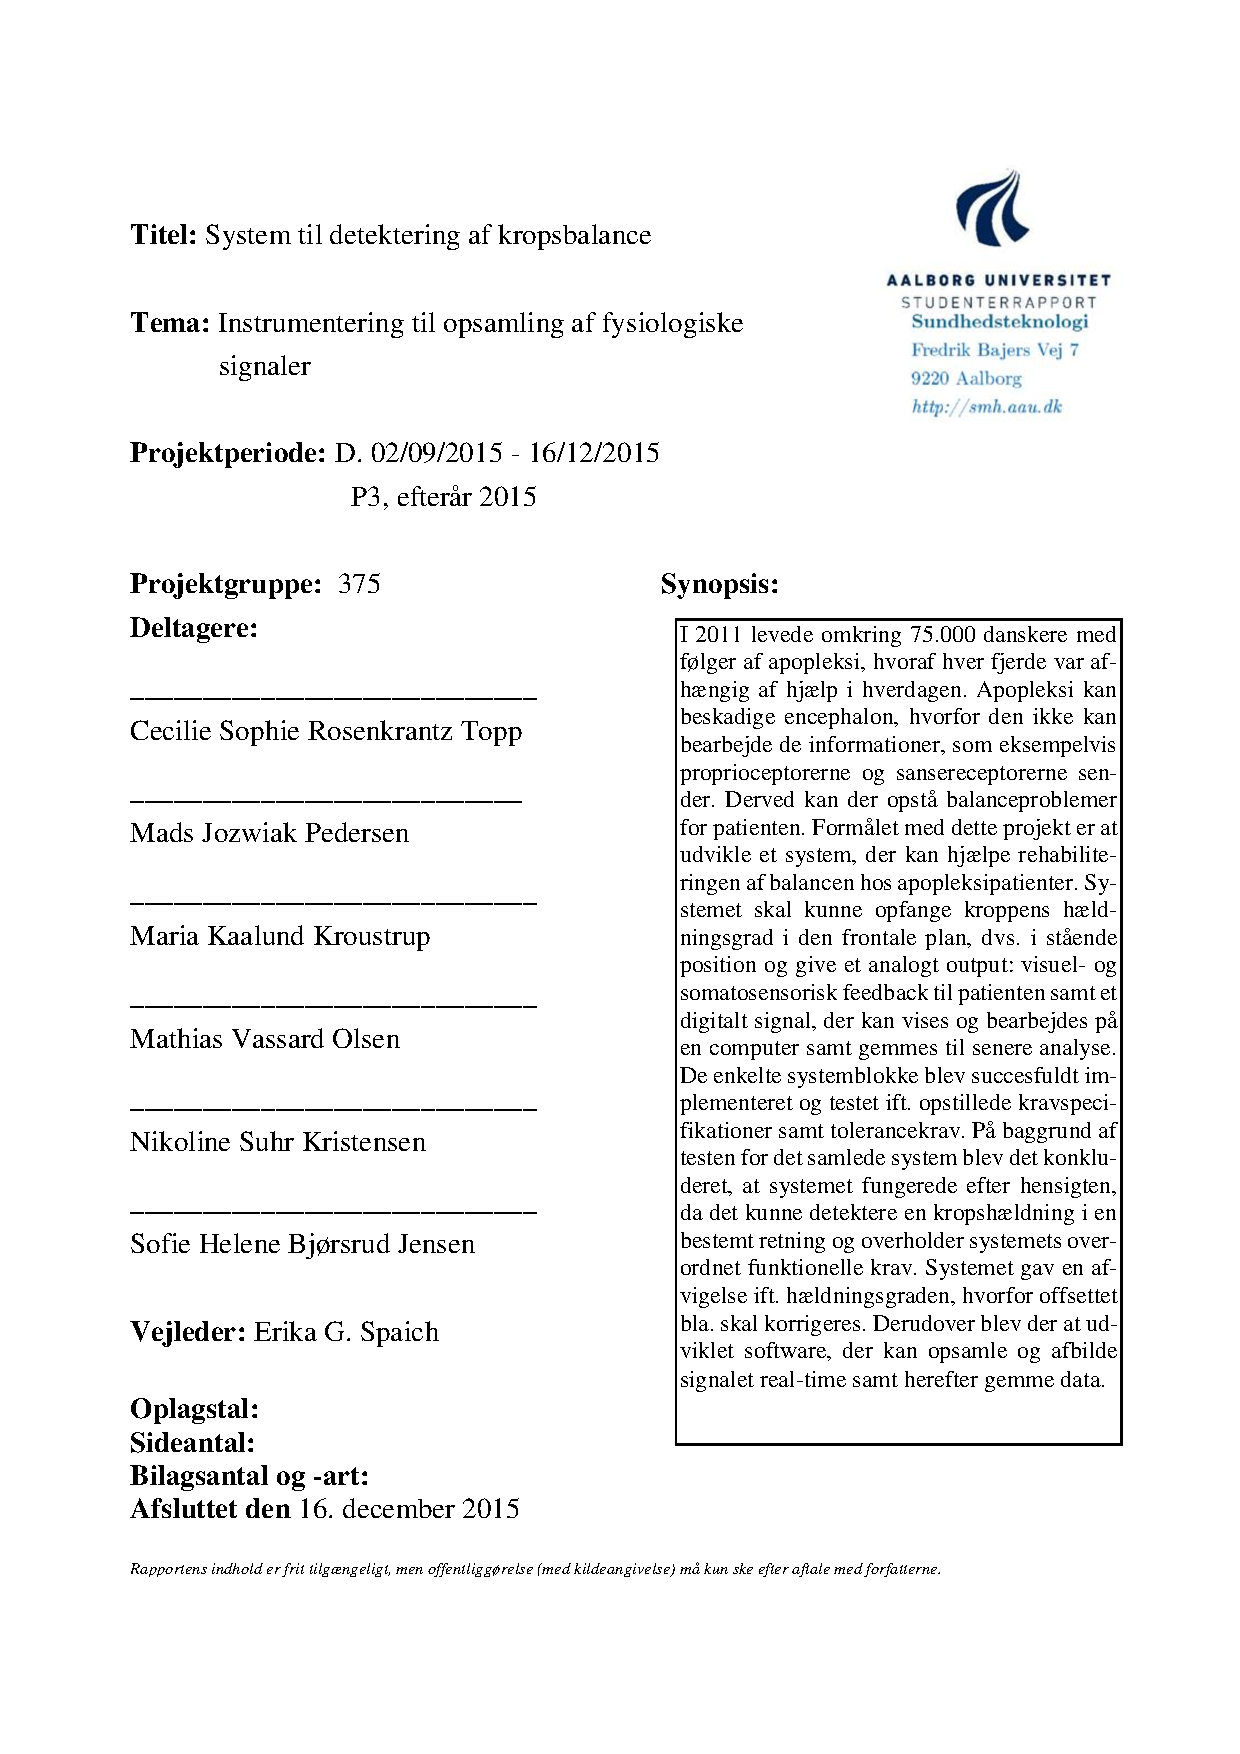
\includepdf[pages={1}]{rapportAfsnit/xFormaliteter/synopsis.pdf} \clearpage 
% !TeX spellcheck = da_DK
\chapter*{Forord og læsevejledning}
\section{Forord}
Denne rapport er udarbejdet i forbindelse med et 3. semester projekt af studerende på Aalborg Universitet,  Sundhedsteknologi af gruppe 15gr375 i efteråret 2015. Ud fra projektets overordnede tema: "Instrumentering til opsamling af fysiologiske signaler" blev der heraf opstillet forskellige projektforslag. Denne rapport vil tage udgangspunkt i følgende projektforslag opstillet af Erika G. Spaich: "System til detektering af kropsbalance". Gruppens vejleder har under hele projektperioden været Erika G. Spaich.

Projektet rettes mod fagkyndigt personale, der beskæftiger sig med rehabilitering af apopleksipatienter og medstuderende på Aalborg Universitet, samt andre, der har interesse i emnet. 
Vi vil gerne takke vores vejleder Erika G. Spaich for vejledning og feedback igennem hele projektperioden. Derudover vil vi give en særlig tak til Jan Stavnhøj for hjælp og rådgivning til udarbejdelse af systemet samt Træningsenhed Vest Aalborg Kommune for at vi måtte komme og observere genoptræning af patienter med balanceproblemer. 

\section{Læsevejledning}
Projektrapporten er baseret på den problembaserede AAU-model. Selve rapporten er delt op i 4 kapitler, samt appendiks, således at første kapitel indeholder projektets initierende problem, der ligger til grund for problemanalysen. Andet kapitel indeholdende problemanalysen giver relevant viden om apopleksi og apopleksipatienternes følger, rehabiliteringsforløb og nuværende rehabiliteringsmuligheder, samt baggrundviden vedrørende teknologisk behandling af biologiske signaler.  Dette er efterfulgt af en projektafgrænsing samt problemformulering, der ligger til grund for problemløsningen. Problemløsningen beskrives i kapitel tre, indeholdende projektets praktiske del ift. at bygge et system til detektering af kropsbalancen. Herunder beskrives systemets kravspecifikationer samt systemdesign, herunder teori, simulering, implementering og test. I fjerde kapitel afsluttes rapporten med en evaluerende diskussion og konklusion af systemets funktion samt perspektivering ift. udvikling af systemet. Herefter findes litteraturlisten, samt appendiks, der henvises til som bilag A, bilag B osv. 

I rapporten benyttes Vancouver-metoden ved litteraturhenvisning, hvor anvendt litteratur tildeles fortløbende numre, således at den første reference i rapporten tildeles nummeret [1], den næste [2] osv. I litteraturlisten skrives den fulde reference, dvs. forfatter navn og årstal samt URL-kode hvis referencen er en hjemmeside, i den rækkefølge referencen anvendes i rapporten. Hvis referencen er placeret efter et punktum i en sætning tilhører referencen hele afsnittet, hvorimod er referencen placeret før et punktum tilhører referencen kun den pågældende sætning. Der der placeret flere referencer efter hinanden betyder dette, at der er anvendt flere referencer til den pågældende sætning eller afsnit. 

Derudover anvendes det amerikanske komma, når der i rapporten skrives tal, eksempelvis 12,500 og 2.4. Dvs. det amerikanske komma på dansk er et punktum og omvendt det amerikanske punktum på dansk er et komma.    

 \clearpage

%the '*' allows the tableofcontents be excepted from the actual table of contents.
\tableofcontents*

%numbers the pages with Arabic numeral - starts from 1.
\mainmatter
\chapter{Indledning}\label{Indledning}
% !TeX spellcheck = da_DK
Apopleksi er pludselig opstået fokalneurologiske symptomer forårsaget af vaskulære forstyrrelser i hjernen, der kan forekomme pga. forhøjet blodtryk, diabetes eller rygning \cite{Sundhedsstyrelsen2009,Academic2015}. Apopleksi er den tredje største dødsårsag i Danmark og ca. 12.500 personer indlægges hvert år pga. sygdommen \cite{Hjernesagen2015a}. Andelen, der dør af hjerneskader, har været stagneret fra 2001 til 2011, hvor 14 \% døde inden for 30 dage \cite{Hjernesagen2015}. Derudover levede 75.000 danskere i 2011 med følger af apopleksi, og ud af disse er omkring hver fjerde person afhængig af hjælp for at kunne udføre dagligdagens gøremål \cite{Hjernesagen2015a}. Antallet af indlæggelsesforløb for mænd og kvinder stiger, når de bliver ældre end 65 år \cite{Sundhedsstyrelsen2011}.
Danskere der lever med følger og varige mén af apopleksi forventes at være stigende i takt med, at der kommer flere ældre \cite{Sagen2014}. Apopleksi er den sygdom, der kræver flest plejedøgn i sundhedssektoren. Ud fra et økonomisk perspektiv er det derfor dyrt for samfundet ift. omkostningerne til behandling, rehabilitering og produktivitetstab.  Udgifterne til sygdommen udgør 4\% af sundhedsvæsenets samlede udgifter, hvor direkte udgifter er estimeret til 2.7 milliard kroner om året \cite{Hjernesagen2015a, Kruuse2014}.
 
%I 2010 var der som sagt 18.041 indlæggelsesforløb forbundet med hjerneskade i Danmark, og det er langt fra alle, som slipper for varige mén heraf\cite{Sundhedsstyrelsen2011}. % gentagelse af det der skrevet før.
Følgerne af apopleksi opstår ofte pludseligt og kan både opleves som fysiske og mentale skader \cite{Muus2008}. Et af de hyppigste mén, som apopleksipatienter oplever, er neglekt. Patienter med neglekt er ikke opmærksomme på den ene side af kroppen \cite{Sundhed.dk}. Derudover opleves sensoriske- og motoriske skader herunder balanceproblemer. De nævnte følger har alle alvorlige konsekvenser for apopleksipatienters livskvalitet, da det bl.a. kan føre til  begrænsninger i hverdagen og i nogle tilfælde faldulykker. \cite{Muus2008,Nichols1997}

De fysiske- og mentale konsekvenser af sygdommen gør, det svært for en apopleksipatient at vende tilbage til sin normale hverdag. Problemer med balancen gør det f.eks. svært at udføre almindelige huslige pligter som rengøring og personlig pleje. \cite{Sundhedsstyrelsen2010} \\
Hjerneskadede patienter, heriblandt apopleksiramte, oplever nedsat livskvalitet pga. deres sygdom. Dette kan ses ved, at apopleksipatienter har dobbelt så stor selvmordsrate som baggrundsbefolkningen \cite{Sundhedsstyrelsen2010}. I en kvantitativ undersøgelse nævner 16\% af apopleksipatienter, at deres livskvalitet er dårlig	\fxnote{46\% nogenlunde, 38\% god} \cite{Sundhedsstyrelsen2010}. Den nedsatte livskvalitet kan føre til vanskeligheder senere i livet \fxnote{Måske skrive hvorfor}. En forbedret livskvalitet kan skabes ved hurtigere rehabilitering eller forbedret kropslige funktioner, som den apopleksiramte mistede ved hjerneskaden. \cite{Sundhedsstyrelsen2010}

For at patienterne opnår den bedst mulige behandling og rehabilitering er det afgørende, at der er et fungerende sammenspil mellem kommuner, sygehuse og praktiserende læger. Apopleksipatienter er krævende ift. rehabilitering pga. omfattende følger efter hjerneskaden. \cite{Sundhedsstyrelsen2010} Det er derfor vigtigt, at fokusere på patienternes rehabilitering for at kunne genoptræne de forskellige fysiske- og mentale mangler de oplever i dagligdagen samt give dem større livskvalitet. 

%Akut behandling og rehabilitering afhænger organisatorisk af hinanden, da sammenspillet mellem kommuner, sygehuse og praktiserende læger er afgørende. % Apopleksi har omfattende og alvorlige konsekvenser og der er derfor brug for involvering fra flere sundhedsprofessionelle områder.\cite{Sundhedsstyrelsen2010}
%De omfatende og alvorglige konsekvenser samt sammenspillet mellem sundhedsområder og rehabilitering er bl.a. det, som gør, at apopleksi er omkostningsfuldt for samfundet.\cite{Sundhedsstyrelsen2010} \\
%Apopleksi påvirker patienters livskvalitet og identitet, da det er svært for patienterne at forholde sig til sygdommen og derved påvirker deres humør, personlighed, færdigheder og sociale relationer. Det er derfor vigtigt at genoptræne patienterne ved at rehabilitering for, at de kan genfinde eller forbedre deres tabte funktioner, f.eks. ved brug af teknologier, som på denne måde er med til at genoprette identitet samt forbedre livskvaliteten for patienten.\cite{Sundhedsstyrelsen2010} 

%Det vil derfor kunne forventes, at der er flere, som kommer ud for en hjerneskade og vil have varige mén herefter, hvilket gør det vigtigt at fokusere på rehabiliteringen for at kunne genoptræne de forskellige kropslige- og mentale mangler.

%%%%%%%%%%%%%%%   Marias foreslag til indledning
%Det kræver samarbejde fra flere professionelle plejepersonale som kommuner, sygehuse og praktiserende læger for at give patienten den rette rehabilitering, da apopleksi patienter er omfattende og kan have alvorlige konsekvenser. Dette gør også at apopleksi er omkostningsfuldt for samfundet. 
% !TeX spellcheck = da_DK
\section{Initierende problem}
Hvilke fysiologiske konsekvenser kan apopleksi have for patienten, og hvad er rehabiliteringsmulighederne for en patient med balanceproblemer? 

%%%%%%%%%%%%%% FORESLAG TIL ANDRE INITIERNEDE PROBLEMER, DER ER MERE PROBLEMORIENTERET %%%%%%%%%%%%%
% 

\chapter{Problemanalyse}
\section{Apopleksi}

Et apopleksi tilfælde kan være forårsaget af enten en blodprop i hjernen (iskæmisk) eller hjerneblødning (hæmoragisk).
Apopleksi er af World Health Organization (WHO) defineret som pludseligt opstået fokale neurologiske symptomer pga. forstyrrelser i hjernens blodcirkulation, der varer mere end 24 timer eller fører til døden[1]. Hvis varigheden er under 24 timer, betegnes det som transitorisk cerebral iskæmi (TCI), hvor de fleste tilfælde varer under 1 time[2] uden permanent hjerneskade [3].

(Billeder)

Iskæmisk apopleksi forekommer hyppigst%ift. hvad? 
[2] og opstår, når en hjernearterie blokeres af en blodprop (infarkt), der stopper tilførslen af blod til et bestemt område i hjernen, hvilket ses på figur xx. Infarkterne dannes primært pga. åreforkalkning enten ved en trombe, der dannes på stedet, eller emboli fra hjertet. Nervecellerne skades efter få minutter pga. stoppet blodtilførsel og vil gå tabt [5].

Hæmoragisk apopleksi skyldes hovedsageligt forhøjet blodtryk eller i sjældnere tilfælde bristede svagheder på arterier (aneurismer) eller misdannede kar[5]. Hæmoragisk apopleksi opstår, når en hjernearterie brister og lækage af blod danner en blodansamling (hæmatom), der beskadiger det omkringliggende væv og forøger trykket i hjernen, hvilket ses på figur xx. Blødning i selve hjernen (intracerebral hæmoragi) kommer af forhøjet blodtryk, der danner et pres på de små arterier, som får dem til at briste[4] og forekommer i 10-12\% af tilfældene[2]. %ift. hvilke tilfælde? 
Blødning i rummet mellem de to hjernehinder (subaraknoidalrummet) skyldes bristning af et aneurisme på en pulsåre i hjernen [5] og forekommer 3-5\% af tilfældene[2]. Symptomerne ved subaraknoidalblødning er generel tab af hjernefunktion, da der forekommer et øget pres på hjerneskallen, hvorimod ved intracerebral hæmoragi er hæmatomet lokaliseret et bestemt sted i hjernen og forårsager nedsat funktion ved én bestemt hjernefunktion[4]. 

% WHO - find en dansk difination istedet.
% Fjern paranteserne - skrev enten det rigtige ord først eller lav en anden måde at skrive det på.
% Mangler lidt en forklaring på, hvordan og hvorfor apopleksi det opstår. Man kan godt uddybe mere i det, der allerede er skrevet.
% Når der er bygget mere på, kan man godt lave nogle forskellige overskrifter.
% Fakta omkring, hvad der er årsagen til apopleksi - hjertesagen har nogle forksellige info om det. Fakta om apopleksi.
% !TeX spellcheck = da_DK
\subsection{Påvirkning på encephalon}\label{HjerneSenMot}
Cerebrum er den største region af encephalon, hvor der sker en processering af sanserne, tale, tanker, synet, hukommelsen og følelser. \cite{Martini2012} Jævnfør afsnit \ref{IskaemiskApp}, side \pageref{IskaemiskApp} er $80$-$85\%$ af apopleksitilfældene iskæmiske og rammer hyppigst i media arterien, der forsyner det meste af cerebrum med blod. Derfor er det ofte sensoriske og motoriske områder, der skades ved et apopleksitilfælde. \cite{Sundhed.dk2014,Kruuse2015a,Gade2004,Boss2010} En yderligere beskrivelse af encephalons anatomi kan ses i bilag \ref{AppNerve} på side \pageref{AppNerve}. For at opretholde balancen kræves et samarbejde mellem de sensoriske og motoriske områder i encephalon, som ses på \figref{Enc}.

\begin{figure}[H]
	\centering
	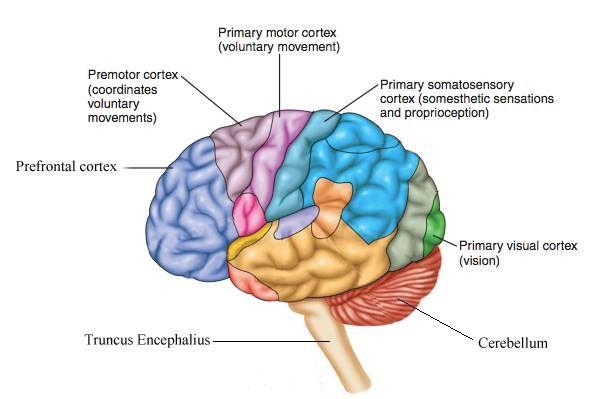
\includegraphics[scale=0.8]{figures/bProblemanalyse/Encephalon3.jpg}
	\caption{På figuren ses de sensoriske og motoriske regioner på den venstre hjernehalvdel af cerebrum. Derudover ses cerebellum og truncus encephalius. \textit{(Revideret)} \cite{Stanfield2014}}
	\label{Enc}
\end{figure}

\noindent De sensoriske og motoriske områder har indflydelse på hinanden. I \tableref{tabelencephalon} beskrives de områder i encephalon illustreret på \figref{Enc}, der har indvirkning på balancen samt funktionen af disse. Ved apopleksi kan flere områder blive beskadiget, hvilket kan medføre, at flere funktioner svækkes. Da balancen kontrolleres af flere forskellige områder i encephalon, betyder en skade på eksempelvis det visuelle cortex ikke, at balancen mistes helt. 

\begin{table} [H]
	\centering
  \begin{tabular}{ | l | p{10cm} |} \hline
    \textit{Område i encephalon} & \textit{Balancefunktioner} \\ \hline
 	Cerebellum & Modtager proprioreceptiv og vestibulær information fra medulla spinalis og truncus encephalius.  Fortolker og koordinerer frivillige bevægelser. \\ \hline
 	Det visuelle cortex & Fortolker lyssignaler, videresender informationer omkring rumlige forhold, bevægelse og koordinerer visuelle og somatosensoriske impulser. \\ \hline
 	Det præmotoriske cortex & Integrerer de sensoriske og motoriske systemer og igangsætter bevægelse som respons på visuelle eller auditive stimuli. \\ \hline
 	Det præfrontale cortex & Koordinerer information fra de andre cortex og udarbejder abstrakte intellektuelle funktioner som at forudse, hvilken effekt en handling vil have. Bearbejder eksterne sanseindtryk inden der foretages en handling. \\ \hline
 	Truncus Encephalius & Modtager vestibulær information fra det indre øre, som fortæller om hovedets placering i rummet og generel balance ift. til tyngdekraften. \\
    \hline
    \end{tabular}
    \caption{På tabellen ses en oversigt over de områder af encephalon, som påvirker balancen, samt deres funktioner. Områderne kan ses på \figref{Enc} \cite{Martini2012, Moos2010}}
    \label{tabelencephalon}
\end{table}
Nervebanerne fra hhv. sensorisk og motorisk cortex løber ned gennem medulla spinalis og leder derved impulser ud til targetorganer og muskler og tilbage igen. Nervebanerne fra hhv. højre og venstre hjernehalvdel krydser i medulla oblongata eller i medulla spinalis. Krydsningen medfører, at afferente signaler fra højre side af kroppen behandles i venstre hjernehalvdel, der sender efferente signaler tilbage til højre side af kroppen. \cite{Martini2012,Stanfield2014} Dette medfører, at et apopleksitilfælde i højre hjernehalvdel kan give sensoriske og motoriske skader i venstre kropsdel og omvendt for venstre hjernehalvdel. \cite{Nichols1997,Sundhedsstyrelsen2009} %Et apopleksitilfælde kan derved lede til neglekt eller problemer med balancen .

Hver muskelgruppe har sine egne dedikerede nerveceller. Antallet af nerveceller til hver muskel afhænger af, hvor kontrolleret muskelgruppens bevægelse skal være. Flere nerveceller øger præcisionen af musklens bevægelse. \cite{Stanfield2014} Nerveceller har en bestemt placering i cerebral cortex. Derfor vil et apopleksitilfælde et bestemt sted ramme en bestemt muskel. F.eks. vil en skade på det auditive cortex muligvis medføre balanceproblemer, da det derved er svært for patienten at vide, hvor hovedet er placeret i rummet. \cite{Mao2014} %Efter et apopleksitilfælde har encephalon en naturlig tilpasningsevne ift. at genskabe disse tabte funktioner. I nogle tilfælde kan encephalon genskabe skadede nerver eller finde en anden vej for funktionen, som en eventuelt tabt nerve skulle udføre. \cite{Martini2012} Denne mekanisme kaldes plasticitet \cite{Ramanathan2006}. 

\subsection{Plasticitet}
Efter et apopleksitilfælde har encephalon en naturlig tilpasningsevne ift. at genskabe disse tabte funktioner. Encephalon kan ændre eller tilpasse sig de stimuli, den udsættes for, hvilket kaldes encephalons plasticitet eller nerveplasticitet. Processen sker kontinuerligt igennem hele livet, men encephalon kan ikke danne nye nerver. \cite{Stanfield2014} Under et apopleksitilfælde forekommer der iltmangel til encephalon, hvilkens kan skader nervecellerne eller resultere i celledød \cite{Schulze2011}. Dette medfører, at den døde nerve mister sine forbindelser til fungerende nerver. Denne forbindelsesafbrydelse i encephalon bevirker, at der kan opstå en kaskade af mistet kommunikation i de eksisterende nerver. Herved kan en nerves celledød påvirke andre områder af encephalon end det sted, hvor skaden er sket. \cite{Raine2009} Encephalon benytter sig af sin plasticitet således, at omlægge det eksisterende nervenetværk til et nyt. Der aktiveres signalstoffer, som kan finde alternative metoder til at gennemføre den ønskede handling. \cite{Rugnett2015} Encephalon kan ikke danne nye nerver efter celledød, hvilket betyder, at der ikke kan generhverves præcis samme funktion som tidligere. En evt. lignende funktion kan generhverves ved gentagende træningsøvelser og kan deles op i følgende fænomener: \cite{Raine2009}

\begin{itemize}
	\item Denervation Supersensitivity: Sker ved en afbrydelse imellem akson og synapse og medfører, at synapsen bliver overfølsom og derved lettere påvirket til at indgå nye synapseforbindelser.
	\item Unmasking of Silent Synapses: Sker når synapser, der tidligere ikke havde en funktion, tilgås og der herved skabes nye funktioner.
	%Sker når synapser med fuld funktionalitet, men ingen effekt på slutstedet, afsløres, hvorefter der opstår en aktivitet og effekt. Dvs. synapsen fungerer, men encephalon er ikke opmærksom på dette.
	\item Collateral Sprouting: Sker hvis to nerver innerverer på samme slutsted, og den ene nerve dør, vil den anden nerve spire ind i den skadede nerves telodendron, så funktionen genvindes.
\end{itemize}

\noindent Ud fra disse fænomener findes der en fysiologisk baggrund for rehabilitering. Forekomsten af nerveplasticitet er særlig øget op til en måned efter et apopleksitilfælde. Det er derfor vigtigt at foretage genoptræning i denne periode, så encephalon kan danne nye forbindelser og kommunikationsveje. \cite{Rugnett2015} Gentagelser af en færdighed effektiviserer synapseforbindelser, hvilket betyder, at den kompenserende færdighed styrkes \cite{Stanfield2014}. En kompenserende færdighed dækker over de kompenserende bevægelser, som kroppen skaber for at erstatte en tabt funktionsevne \cite{Takeuchi2012,Leea2009}.

Nerveplasticitet betragtes ikke kun som en positiv egenskab. Plasticiteten gør encephalon fleksibel for omlægning efter en skade, men også sårbar overfor udefrakommende og interne ubevidste påvirkninger. Dårlige vaner er en negativ egenskab ved plasticitet, fordi gentagende hændelser, der frigiver dopamin, også giver stærke synapseforbindelser. Når mennesker forsøger at slippe af med en vane, som f.eks. rygning, vil det neurale kredsløb i encephalon blive svagere, men det findes stadig og kan genaktiveres, hvormed vanen kan genoptages. \cite{Hampton2015}

 %Udover plasticitet vil kroppen også skabe såkaldte kompenserende bevægelser for at erstatte en tabt funktionsevne. %Kompensatoriske bevægelser er et resultat af, at kroppen stadigvæk har brug for en givet funktion, men pga. tabt sensorisk og motorisk funktion ikke kan udføre bevægelsen. Disse kompenserende bevægelsesmønstre kan medføre et funktionelt dårligt resultat og kan være associeret med langsigtede konsekvenser såsom smerte og reduceret funktionsevne \cite{Takeuchi2012,Leea2009}.


%\subsection{Plasticitet}
%Encephalon kan ændre eller tilpasse sig de stimuli, den udsættes for, hvilket kaldes encephalons plasticitet eller nerveplasticitet. Dette sker kontinuerligt igennem hele livet, men encephalon kan ikke danne nye nerver. \cite{Stanfield2014} Under et apopleksitilfælde forekommer der iltmangel til encephalon, og nervecellerne kan derved blive skadet eller gå tabt. \cite{Schulze2011} Denne celledød gør, at den døde nerve mister sine forbindelser til raske nerver. Denne forbindelsesafbrydelse i encephalon bevirker, at der kan opstå en kaskade af mistet kommunikation i de eksisterende nerver. Herved kan en nerves celledød altså påvirke andre områder af encephalon end blot der, hvor skaden er sket. \cite{Raine2009} Encephalon vil benytte sig af sin plasticitet og omlægge det eksisterende nervenetværk. Encephalon vil aktivere nogle signalstoffer, som kan finde en alternativ metode til at gennemføre den ønskede handling. \cite{Rugnett2015}  Som sagt kan encephalon ikke danne nye nerver efter celledød, hvilket betyder, at der ikke kan generhverves præcis samme funktion som tidligere men evt. en lignende funktion. Men encephalon vil forsøge at kompensere for de tabte nerver ved at danne nye forbindelser og kommunikationsveje, hvilket kan deles op i tre fænomener: \cite{Raine2009}

%\begin{itemize}
	%\item En afbrydelse imellem akson og synapse medfører, at synapsen bliver overfølsom og derved lettere påvirket til at lave nye synapseforbindelser. Dette fænomen kaldes “Denervation Supersensitivity”.
%	\item Synapser, der har fuld funktionalitet men ingen effekt på slutstedet, “afsløres”, hvorefter der opstår en aktivitet og effekt. Dette kaldes “Unmasking of Silent (Latent) Synapses”.
%	\item Hvis to nerver innerverer på samme slutsted, og den ene nerve dør, så vil den anden nerve spire ind i den skadede nerves telodendron, og funktionen vil derved genvindes. Dette kaldes “Collateral Sprouting”.
%>>>>>>> origin/master
%\end{itemize}

%det forrige
%\subsection{Påvirkning på encephalon}\label{HjerneSenMot}

%Cerebrum er den største region af encephalon og kan deles op i to hjernehalvdele. Her sker en processering af sanserne, tale, tanker, synet, hukommelsen og følelser. \cite{Martini2012} For en yderligere beskrivelse af hjernen, nervefysiologi samt biologisk kommunikation se bilag \ref{AppNerve}. De forskellige sensoriske- og motoriske regioner kan ses på \figref{Enc}. Som tidligere nævnt i afsnit \ref{IskaemiskApp} er 80-85\% af apopleksitilfældene iskæmiske og rammer hyppigst i media arterien, der forsyner det meste af cerebrum med blod. Derfor er det ofte sensoriske- og motoriske områder, som bliver skadet ved et apopleksitilfælde. \cite{Sundhed.dk,Gade2004,Boss2010} \\

%\begin{figure}[H]
%	\centering
%	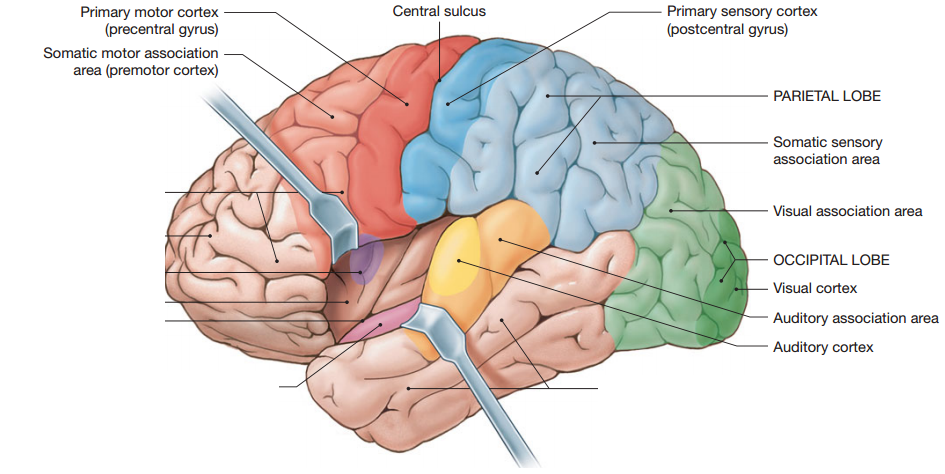
\includegraphics[scale=0.6]{figures/bProblemanalyse/Encephalon.png}
%	\caption{På figuren ses de sensoriske og motoriske regioner på den venstre hjernehalvdel af cerebrum. %\textit{(Revideret)} \cite{Martini2012}}
%	\label{Enc}
%\end{figure}

%De sensoriske- og motoriske nervebaner fra sensorisk- og motorisk cortex løber ned gennem medulla spinalis og leder derved impulser ud til target organer og muskler og tilbage igen. Nervebanerne fra hhv. højre og venstre hjernehalvdel krydser i medulla oblongata eller i medulla spinalis. Denne krydsning betyder, at afferente signaler fra højre side af kroppen behandles i venstre hjernehalvdel, der sender efferente signaler tilbage til højre side af kroppen. \cite{Martini2012,Stanfield2014} Dette medfører, at et apopleksitilfælde i højre hjernehalvdel kan give sensoriske- og motoriske skader i venstre kropsdel og omvendt med venstre hjernehalvdel. \cite{Sundhedsstyrelsen2009,Nichols1997} %Et apopleksitilfælde kan derved lede til neglekt eller problemer med balancen .

%Hver muskelgruppe har sine egne dedikerede nerveceller. Antallet af nerveceller til hver muskel afhænger af, hvor præcis legemets bevægelse skal være. Flere nerveceller gør musklens bevægelse mere præcis. \cite{Stanfield2014} Nervecellerne har en bestemt placering i cerebral cortex. Derfor vil et apopleksitilfælde et bestemt sted ramme en bestemt muskel. F.eks. vil en skade på det auditive cortex kunne medføre balanceproblemer, da det derved er svært for patienten at vide hvor hovedet er placeret i rummet. \cite{Mao2014} 
%\begin{center}
%\begin{tabular}{ | l | p{8cm} |}
%\hline
%Auditive cortex & hej med dig \\ \hline
%\end{tabular}
%\end{table}

%\subsection{Encephalons påvirkning på balance}
%For at opretholde balancen kræves der samarbejde af flere områder af encephalon. Disse har en stor indflydelse på hinanden. Områderne kan ses i \tableref{tabelencephalon}. Ved apopleksi kan flere områder rammes samtidig, hvilket kan gøre at flere funktioner svækkes. Da balancen er styret af flere forskellige områder i encephalon betyder en skade på eksempelvis det visuelle cortex ikke at man mister balancen helt. 

%\begin{center}
%\begin{table} [H]
  %\begin{tabular}{ | l | p{8cm} |}
   % \hline
  %  \textbf{Område i encephalon} & \textbf{Funktioner} \\ \hline
 %	Cerebellum & Modtager proprioreceptiv og vestibulær information fra medulla spinalis og truncus encephalius.  %Fortolker og koordinerer frivillige bevægelser. \\ \hline
 %	Det visuelle cortex & Fortolker lyssignaler og videresender informationer omkring rumlige forhold, bevægelse og %koordinerer visuelle og somatosensoriske impulser. \\ \hline
 %	Det præmotoriske cortex & Integrerer den sensoriske og motoriske systemer og igangsætter bevægelse som respons på %visuelle eller auditive stimuli. \\ \hline
 %	Det præfrontale cortex & Koordinerer information fra de andre kortex og udarbejder abstrakte intellektuelle %funktioner, som at forudse hvilken effekt en handling vil have. Bearbejdere eksterne sanseindtryk inden der foretages %en handling. \\ \hline
 %	Truncus Encephalius & Modtager vestibulær information fra det indre ører, som fortæller hovedets placering i %rummet og generel balance ift. til tyngdekraften. \\
    %\hline
   % \end{tabular}
 %   \caption{Tabel over de områder af encephalon som påvirker balancen, samt deres funktion. \cite{Martini2012, %Moos2010}}
 %   \label{tabelencephalon}
%\end{table}
%\end{center}


%Encephalon har en naturlig tilpasning. Dette medfører, at den i nogle tilfælde kan genskabe skadede nerver eller finde en anden vej for funktionen, som en eventuelt tabt nerve skulle udføre. \cite{Martini2012} Denne mekanisme kaldes plasticitet \cite{Ramanathan2006}.
% !TeX spellcheck = da_DK
\section{Behandlinger}
Når en patient rammes af apopleksi, er det vigtigt at komme i behandling hurtigst muligt. Ved ankomst på sygehuset foretages der en scanning af encephalon for at undersøge, hvorvidt det er iskæmisk eller hæmoragisk apopleksi. Hvis hæmoragisk apopleksi findes der endnu ingen akut behandling, der kan stoppe blødningen.\cite{Soenderborg2013} Hvorimod ved akut iskæmisk apopleksi, hvilket vil sige at symptomerne er til stede inden for fire en halv time, anvendes blodpropopløsende medicin. Ved hurtig behandling vil det være muligt at opløse blodproppen. I andre tilfælde fjernes blodproppen ved brug af et tyndt kateter, som indføres gennem arterien op til encephalon. Derudover anvendes blodfortyndende medicin for at undgå nye tilfælde af apopleksi. \cite{Hjerteforeningen2014, Kruuse2014a} 

%\subsection{Akut behandling}
%Ved mistanke om iskæmisk apopleksi er det vigtigt, at der tages kontakt til sygehuset omgående. Patienten bliver her undersøgt ved blodtryksmåling, blodprøver, neurologisk undersøgelse og scanning af encephalon. Dermed kan det udelukkes om der er eventuelle blødninger eller andre årsager til funktionstabet. Dette  sikrer, at patienten får den rette behandling. I tilfælde af blodprop igangsættes en behandling med blodpropopløsende eller blodpropshæmmende medicin. \cite{Hjerteforeningen2014, Kruuse2014a} 
%
\subsection{Trombolyse}
Standardbehandling for blodpropper har siden år 2006 været trombolyse. Selve behandlingen foregår ved, at der sprøjtes blodpropopløsende medicin ind i en arterie, ofte i armen, hvorefter blodproppen opløses. Denne behandling skal helst foregå seks timer efter blodproppens forekomst og senest 12 timer efter, da behandlingen ikke vil have nogen indvirkning efter længere tid. Hurtig behandling vil betyde at flere områder af encpehalon vil kunne reddes. Dermed vil patientens fremtidige livskvalitet forbedres. Trombolysebehandlingen finder sted på 12 sygehuse fordelt over de fem regioner. En risiko ved behandlingen kan være blødninger grundet den blodpropopløsende medicin. \cite{Hjernesagen2015b}

\subsection{Forebyggelse}
En væsentlig del af behandlingen er forebyggelse, da risikoen for en ny blodprop er betydelig. Til forebyggelse anvendes antikoagulationsbehandling, som er en behandling med blodfortyndende medicin. Normalt har kroppen sit eget koagulationsssystem som får blodet til at koagulere. Derudover medvirker koagulationssystemet også til at opløse evt. blodpropper i det kardiovaskulæresystem. For apopleksipatienter fungerer koagulationssystemet ikke optimalt, hvilket gør det nødvendigt at behandle med antikoagulation. Dette hæmmer blodets evne til at koagulere, hvilket modvirker dannelsen af blodpropper. Der findes to former for antikoagulationsbehandling, warfarin og nyre orale antikoaglulantia. Den primære forskel mellem de to mediciner er, at der ved behandling med nyre orale antikoaglulantia ikke kræves kontrol ved blodprøver.\cite{Kjaergaard2015}

%[1]http://www.hjerteforeningen.dk/alt-om-dit-hjerte/hjerte-kar-sygdomme/apopleksi/
%[2]http://www.hjernesagen.dk/om-hjerneskader/behandling/trombolyse
%[3] https://www.sundhed.dk/borger/sygdomme-a-aa/hjerte-og-blodkar/sygdomme/apopleksi/behandling-ved-apopleksi/
%[4]https://www.sundhed.dk/borger/sygdomme-a-aa/hjerte-og-blodkar/sygdomme/behandlinger/antikoagulationsbehandling-blodfortyndende-medicin/
\input{rapportAfsnit/cProblemanalyse/Foelger}
% !TeX spellcheck = da_DK
\section{Rehabilitering}
Når selve slagtilfældet er stabiliseret og behandlet, er det essentielt, at rehabiliteringen af en apopleksipatient indfindes hurtigst muligt - gerne en til to dage efter slagtilfældet. I Danmark dækker rehabilitering af en patient med apopleksi områderne: direkte træning af funktioner, ufrivillig reorganisering af hjernen netværk, kompenserende strategier, ændringer i miljø, social og psykologisk støtte. Genoptræningen omhandler dog ikke kun træning med en ergo- eller fysioterapeut, da plejepersonale til dagens almindelige gøremål også essentiel. Patientens daglige rutiner kan være gået tabt under slagtilfældet, hvorfor det er vigtigt, at få patienten tilbage i sit vante miljø. Plejepersonale skal hjælpe patienten til at genfinde denne rytme og hjælpe patienten til eventuelt at udføre dagligdags ting på en ny måde. Det kan ske, at patienten ikke længere er i stand til at beherske begge sine hænder til en opgave, hvorved plejepersonalet skal bistå patienten i indlæringen af kun at benytte en hånd.

Motoriske og sensoriske funktionsproblemer kan lede til balancebesvær for patienten i både siddende, stående og gående stilling. Der er afprøvet adskillige farmakologiske midler og behandlingsstadegier for at forbedre hjernens rehabilitering og motoriske funktioner. F.eks. er der afprøvet, at tildele apopleksipatienter det antidepressive middel fluoxetin i kombination med fysioterapi. Derudover er kortikal stimulation afprøvet, hvor området af hjernen, som kontrollerer motorstyring, modtager elektriske impulser fra en implanteret anordning. Denne mulighed har haft blandede succesoplevelser, men er udelukkende afprøvet på patienter, der har oplevet et alvorligt slagtilfælde. \cite{Academic2015}
  
Apopleksi patienten skal i samarbejde med lægen, sygeplejersken og andet hjælpepersonale opstille nogle mål for sin rehabilitering. Målene skal hverken være for svære eller for lette, så patienten ikke mister sin motivation til genoptræningen. \cite{Kruuse2015}

\subsection{Forløbsprogram for rehabilitering} 
Sundhedsstyrelsen har udarbejdet et forløbsprogram for rehabilitering af patienter med erhvervet hjerneskade. Forløbsprogrammet strækker sig fra at patienten erhverver hjerneskaden til at patienten har opnået bedst mulig funktionsevne, hvorefter der udføres kontrol og vedligeholdelse af funktionsevnen. Tidsperioden af rehabilitering varierer ift. hjerneskadens sværhedsgrad, samt sværhedsgraden af funktionstabet. %dog kan perioden vare flere år.  
\cite{Sundhedsstyrelsen2011a}

Forløbsprogrammet er essentielt i forhold til at kunne give patienten den korrekte rehabilitering. Patienterne har forskellige behov og er afhængige af hjælp fra plejepersonale. Deruodver kræves der forskellige former for teknologi i de forskellige faser. Det vil derfor være oplagt at undersøge, hvilken form for rehabilitering der er at foretrække i de enkelte faser som ses på \figref{firefaser}.

\begin{figure}[H]
	\centering
	\includegraphics[scale=0.6]{figures/bProblemanalyse/flowdiagram_faser1.png}
	\caption{På figuren ses et overblik over de fire faser, som patienter med apopleksi skal igennem i forløbsprogrammet for rehabilitering \cite{Sundhedsstyrelsen2011a}} 
	\label{firefaser}
\end{figure}

\subsubsection{Den første fase}
Som det vises på \figref{firefaser} afspejler første fase den del af forløbsprogrammet som foregår på sygehusets apopleksiafdeling. På apopleksiafdelingen foretages primært akut behandling for at begrænse skaderne. Når patientens sikkerhed er sikret og skaderne er begrænset påbegyndes den tidlige rehabilitering. Under den tidlige rehabilitering giver en speciallæge i neurologi en vurdering af patientens rehabiliteringsbehov. Derudover bliver patienterne overvåget i forhold til bevidsthed, ændringer og amnesi samt foretaget vurderinger af basale fysiologiske funktioner. Samtidig bliver der iværksat træning i diverse bevægelsesfunktioner, basale egenskaber og kommunikationsfunktioner. Patienterne gennemgår også en tidlig behandling og diagnostik for at undersøge komplicerende tilstande, som f.eks. vaskulære hændelser, blodpropper i ben og lunger og smerter. Patienterne vurderes i denne fase af fagkyndigt personale som ergoterapeut, fysioterapeut og audiologopæd \fxnote{høre og talepædagog}. Disse er med til, at sikre, at patienten udfører træningen korrekt i forhold til stilmulering og træning af bevægelsesfunktioner, taletræning og udførsel af basale daglige aktiviteter.\cite{Sundhedsstyrelsen2011a}

\subsubsection{Den anden fase}
Det fremgår af \figref{firefaser}, at patienten i den anden fase gennemgår rehabilitering på sygehuset, hvor der er fokus på de skadede funktioner. Ligeledes bliver patienten på samme måde som i fase et undervist af fagkyndigt personale. Hvorefter patientens behov for rehabilitering og rehabiliteringens udvikling vurderes. Patienterne bliver i denne fase udredet i forhold til funktionsevne, mentale funktioner, bevægelsesfunktioner herunder bevægelse og mobilitet i led, knogler, reflekser og muskler samt rehabilitering med henblik på daglige aktiviteter. Hvis patienten vurderes til at have en stabil udvikling i rehabiliteringsprocessen, vil patienten blive udskrevet og påbegynde fase tre. \cite{Sundhedsstyrelsen2011a}


\subsubsection{Den tredje fase}
I den tredje er patienten udskrevet fra sygehuset. Derved foregår rehabilitering som ambulant rehabilitering og selvstændig træning, som det fremgår af \figref{firefaser}.  Selve rehabiliteringen i tredje fase er bygget op ud fra rehabiliteringsforløbet i den anden fase. Det afgørende for den tredje fase er, hvorvidt patienten skal vedblive rehabilitering på sygehuset eller henvises til de kommunale rehabiliteringscentre. Dette afgøres på baggrund af observationer foretaget i anden fase. Den selvstændige træning kan for patienter med neglekt og balanceproblemer være en udfordring ift. bevægelsesmønstre og kropsholdning. \cite{Sundhedsstyrelsen2011a}

\subsubsection{Den fjerde fase}
Det fremgår på \figref{firefaser}, at fjerde fase er den afsluttende fase for behandlingsforløbet. Patienterne går stadig til kontrol og vedligeholdelse for at sikre, at rehabiliteringens udvikling er stabil. Det kan i sidste ende have betydning for, hvor lang tid det tager for patienten at generhverve sine tabte funktioner. Den fjerde fase varierer derfor fra patient til patient alt efter udviklingen af rehabiliteringen.\cite{Sundhedsstyrelsen2011a} \\

\subsection{Organisatorisk}
Sygehusvæsenet, almen praksis og kommuner har opgaver i alle faser, dog i varierende grad. Således har sygehuset flest opgaver i fase I og II, mens kommunen og almen praksis har flest opgaver i fase III (og IV) \cite{Sundhedsstyrelsen2011a}.

%\section{Organisatorisk}
%I sundhedssektoren arbejder de forskellige organisatoriske aktører på tværs af hinanden. Der er således et samarbejde mellem syghuse, kommuner og praktiserende læger. Dette samarbejde skal ske både internt på syghusene, på afdelingerne og kommunalt mellem forvaltningerne \cite{Sundhedsstyrelsen2010}. Samspillet mellem aktørerne er vigtigt, da patienter med hjerneskade berører flere afdelinger. De har derfor brug for involvering af flere sundhedsprofessionelle grupper under behandling og rehabilitering på grund af de omfattende og alvorlige konsekvenser.

%De ovennævnte aktører er de organisatoriske enheder, der har en central rolle i forløbet. Det er ikke muligt at fastlægge en egentlig organisering af hjerneskaderehabiliteringen i Danmark, da sammenspillet mellem de forskellige aktører er meget flydende og forskellige alt efter hvor i landet man befinder sig og hvor omfattende hjerneskaden er. Denne forskel opleves regionalt, hvor behandling og rehabilitering enkelte steder foregår på få af sygehusets afdelinger, mens patienter andre steder behandles på et rehabiliteringssygehus, efter den akutte behandling er foretaget.\cite{Sundhedsstyrelsen2010}

%I starten af behandlingssforløbet sendes patienterne til neurologiske, geriatriske, neurokirurgiske og medicinske afdelinger på sygehuset. Som tidligere nævnt inddeles patienterne efter sværhedsgrad af hjerneskaden, hvor de sværest ramte, som er patienter med traumatisk hjerneskade og tilgrænsede lidelser, vidererstilles til Hammel og Hvidovre. Rehabiliteringen kan også ske på rehabiliteringsafsnittene på landets sygehuse.
%Det primære ansvar ligger hos kommunerne i form af genoptræningsplanens afdækning af rehabiliteringsbehov, dvs. at kommunerne holder øje med om dette foregår i praksis, herunder bl.a. patientens genoptræningsbehov. Kommunen har derudover mulighed for at henvise patienterne til dens egne tilbud, samt at henvise til private.\cite{Sundhedsstyrelsen2010} 

%Afslutningsvis gennemgår patienterne et langt og forskelligt behandlingsforløb alt efter hjerneskadens omfang. Forløbet indebærer et samarbejde mellem de forskellige aktører. Efter behandlingen står kommunerne, som førnævnt, for det primære ansvar i forhold til rehabilitering og henvisning for patienten\fxnote{hvor kommer denne info fra?}.



% I første og anden fase af rehabiliteringsforløbet bliver patienten undervist og overvåget af fagkyndigt personale. Dette gøres for at sikre, at patienten udfører træningen korrekt f.eks. med bevægelsesmønstre, og korrigere patienten til at bevægelsen og øvelserne udføres korrekt. Dette er vigtigt, da patienten, som sagt i tredje fase, selv skal foretage den nødvendige træning og dermed har fornemmelse af, hvordan træningen udføres korrekt ift. bevægelsesmønstre og kropsholdning. Dette kan midlertidig være en udfordring for apopleksipatienter med neglekt, da de kan have problemer med balancen og opmærksomheden på kroppen. Patienten går derfor stadig til kontrol og vedligeholdelse for at sikre, at rehabiliteringens udvikling er stabil. Det kan i sidste ende have betydning for, hvor lang tid det tager for patienten at generhverve sine tabte funktioner. Den tredje fase varierer derfor fra patient til patient alt efter udviklingen på rehabiliteringen. \cite{Sundhedsstyrelsen2011a}
% !TeX spellcheck = da_DK
\subsection{Nuværende metoder til rehabilitering}

Inden patienten udskrives fra sin behandling skal der fra sundhedssektorens side være udarbejdet en genoptræningsplan. I denne plan besluttes det hvilken form for rehabilitering og teknologi patienten skal benytte sig af. \cite{Sundhedsstyrelsen2011a} \\
Der findes flere forskellige metoder og teknologier til at hjælpe med balance og gangproblemer. Disse omfatter: Platform feedback, fokuseret gangtræning, konditionstræning, auditorisk rytmestøtte, elektromekanisk fysioterapistøttet gangtræning, opgavespecifik repetitiv træning, spejlterapi, programmer til motorisk visualisering og passiv sensorisk stimulation. \cite{Sundhedsstyrelsen2011a}\fxnote{dette skal laves om til punktform.} \\
Platform feedback er en biofeedback metode, hvor patienten står på en platform. Platformen vil herefter måle hvor meget patienten svajer \fxnote{(centre of pressure)}. Når platformen har målt svajningen af patienten, kan denne enten få visuel eller auditiv feedback. Feedbacken skal gøre patienten mere opmærksom på, hvor meget kroppen svajer, hvilket gør det muligt at opretholde en stående position.%[1]
Denne form for teknologi benyttes særligt i de tidlige faser af rehabiliteringen\cite{Sundhedsstyrelsen2011a}. \\
Det er med høj evidens blevet påvist, at fokuseret gangtræning medfører en moderat grad af bedringen på gangfunktionen hos apopleksiramte\cite{Sundhedsstyrelsen2010}. Derudover er det også vist, at konditionstræning kan være med til at forbedre gangfunktionen\cite{Sundhedsstyrelsen2010}. \\
Auditorisk rytmestøtte er en metode, hvor patienten lytter eller udfører handlinger til en form for musik. Det mest centrale ved musikken er rytmen, der findes i den.%[2] 
Det er vist, at denne metode kan øge både ganghastigheden, skridtlængden og gangsymmetrien \cite{Sundhedsstyrelsen2010}. \\
Ved elektromekanisk fysioterapistøttet gangtræning benytter fysioterapeuten sig af en maskine til hjælp af patientens gang. Maskinen består af enten et robot-drevet exoskelet eller to drevne mekaniske plader, der simulerer gang hos patienten. %[3] 
Denne form for metode har vist at kunne øge skridthastighed, skridtlængde og skridtsymmetri \cite{Sundhedsstyrelsen2010}. Denne metode benyttes til patienter med svært nedsat gangfunktion, med særlig fokus på de tidlige faser af rehabiliteringen \cite{Sundhedsstyrelsen2011a}. \\
Opgavespecifik repetitiv træning omfatter aktivitetsbestemte motoriske opgaver, som er bestemt til den enkelte patient. Disse opgaver tager udgangspunkt i hverdagsaktiviteter. Denne metode kan have effekt på patienternes gangfunktion, gangdistance og -hastighed. \cite{Sundhedsstyrelsen2010} \\
Spejlterapi er en træning af bevægelser, hvor patienten laver en række bevægelsesmønstre med den raske side af kroppen. Herefter bliver disse bevægelser spejlet til den syge side af kroppen. Dette vil skabe en illusion af et normalt bevægelsesmønster af den syge side hos patienten. \cite{Sundhedsstyrelsen2010} Denne metode skal tilbydes under hele rehabiliteringen \cite{Sundhedsstyrelsen2011a}.\fxnote{Måske uddybe, hvordan spejlingen foregår..} \\
Programmer til motorisk visualisering kan bl.a. være "virtual reality" \cite{Sundhedsstyrelsen2010}. Dette er en form for program, hvor en computer modellerer og simulerer et miljø, som patienten kan placeres i vha. briller og andre interaktive apparater[4]. Dette gør at patienten kan simulere bevægelser, som de ikke nødvendigvis er i stand til i virkeligheden. Det er uafklaret, hvilken effekt denne form for rehabilitering har \cite{Sundhedsstyrelsen2010}. \\
Passiv sensorisk stimulation er en rehabiliteringsform, hvor patienten modtager elektrisk stimulation, der ikke aktiverer musklerne. Stimulationen er der for at fortælle patienten om, hvad kroppen foretager sig, så det bliver muligt at korrigere bevægelserne. \cite{Sundhedsstyrelsen2010} Denne form for metode tilbydes under hele rehabiliteringsforløbet \cite{Sundhedsstyrelsen2011a}.\fxnote{Dette må også gerne uddybes - hvordan har det en gavnlig effekt at ens muskler ikke aktiveres?}
%
%
%[1] - http://onlinelibrary.wiley.com.zorac.aub.aau.dk/doi/10.1002/14651858.CD004129.pub2/full
%[2] - http://onlinelibrary.wiley.com.zorac.aub.aau.dk/doi/10.1002/14651858.CD006787.pub2/full
%[3] - http://onlinelibrary.wiley.com/doi/10.1002/14651858.CD006185.pub3/full
%[4] - http://academic.eb.com.zorac.aub.aau.dk/EBchecked/topic/630181/virtual-reality-VR/
\input{rapportAfsnit/cProblemanalyse/biofeedback}
% !TeX spellcheck = da_DK
\section{Behandling af kropshældnings signal}
Et biologisk signal skal behandles for at kunne give feedback til patienten samt et digitalt output evt. til plejepersonale. For at kunne behandle et signal fra et accelerometer kræves der bl.a. forstærkning, filtrering, komparator samt ADC. Der kan anvendes andre komponenter til signalbehandling ift. hvad accelerometret skal benyttes til, men de nævnte vil blive benyttet i dette projekt. 

\subsection{Forstærker}\label{forstaerkerafsnit}
En forstærker kan benyttes til at ændre inputtet i form af et biologisk signal til et skaleret output. Dette kan gøres ved at kombinere en operationsforstærker med modstande, der derved kan skalere, invertere, addere og subtrahere signalet. Der findes fire forskellige forstærkningskredsløb til at udføre de nævnte opgaver: \cite{Nilsson2011}
\begin{itemize}
\item Inverterende forstærkningskredsløb: Benyttes til at invertere signalet samtidig med det skaleres.% Inverteringen af signalet betyder, at der ændres fortegn på signalet.
\item Summerende forstærkningskredsløb: Fungerer ligesom det inverterende forstærkningskredsløb med den undtagelse, at inputsignalerne summeres.
\item Ikke-inverterende forstærkningskredsløb: Benyttes til at skalere input signalet.
\item Differens forstærkningskredsløb: Benyttes til at trække to input signaler fra hinanden, så outputsignalet bliver forskellen på de to inputsignaler \cite{Nilsson2011}. Der findes forskellige typer af differensforstærkning, herunder et kredsløb med en enkelt operationsforstærker eller en instrumenteringsforstærker. I instrumenteringsforstærkeren indgår yderligere to operationsforstærkere for at lave inputbuffere til den oprindelige operationsforstærker. \cite{Sedra2010}  
\end{itemize} 

%\noindent For at forstærke signalet fra et accelerometeret benyttes operationsforstærkeren, der skalerer inputspændingen til en ønsket outputspænding. Dette gøres, hvis den næste komponent skal bruge et specifikt input eller for at forstærke signaler med lav amplitude. Der kan f.eks. bruges en inverterende forstærker, som ses på \figref{invf}, hvor $V_{s}$ er det målte signal, der ønskes forstærket og $V_{o}$ er outputsignalet. Inputtets forstærkning kaldes gain og er en ratio mellem $dfrac{R_{f}}{R_{s}}$, som er de to modstande. \cite{Nilsson2011}
%
%\begin{figure}[H]
%\centering
%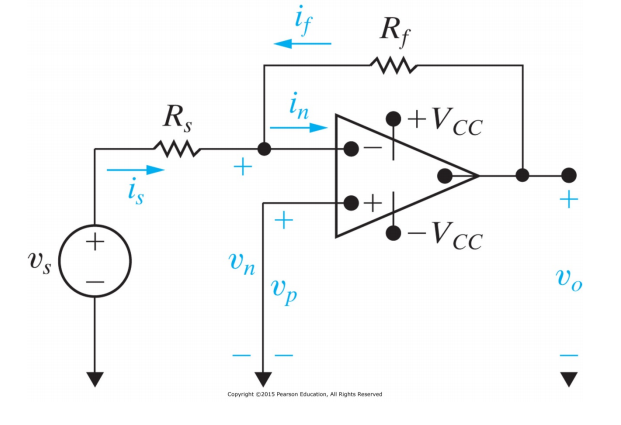
\includegraphics[scale=0.6]{figures/bProblemanalyse/inverterendeforstaerker.png}
%\caption{På figuren ses en ideel operationsforstærker, som er inverterende koblet og kan forstærke input signalet $V_{s}$ til et ønsket output signal $V_{o}$ vha. modstandene $R_ {s}$ og $R_{f}$. \cite{Nilsson2011}}
%\label{invf}
%\end{figure}


%INDLEDE MED KORT FORKLARING PÅ HVAD EN FORSTÆRKER EGENTLIG ER OG HVILKE FORSKELLIGE TYPER DER FINDES
%UNDERSTREGE AT VI GODT VED AT DER ER FLERE FORSKELLIGE TYPER AF FORSTÆRKERE..
% !TeX spellcheck = da_DK
\subsection{Filtrering}
Filtrering er et værktøj indenfor databehandling, som anvendes i det målte signals frekvensdomæne. Formålet med at filtrere et målt signal er at fjerne uønskede frekvenser, også kaldet støj, der ikke tilhører det signal, der ønskes undersøgt. Filtret kan opdele signalet i såkaldte bånd: Pasbånd, hvor frekvenserne frit passerer igennem filteret uden påvirkning, samt stopbånd, hvor frekvenserne dæmpes, så de ikke har indflydelse på signalet. Dette gøres ved en knækfrekvens.
Der findes flere forskellige typer af filtre, som ses på \figref{filtertyper}, der afhænger af, hvilke frekvenser der skal fjernes fra det målte signal \cite{Devasahayam2000}:

\begin{itemize}
	\item Lavpasfiltret: Anvendes til at dæmpe frekvenser over den valgte knækfrekvens. Dette gøres ved at dæmpe de frekvenser, som ligger over knækfrekvensen.
	\item Højpasfilteret: Anvendes, modsat lavpasfiltret, til at dæmpe frekvenser under den valgte knækfrekvens ved at dæmpe signalet under knækfrekvensen.
	\item Båndpasfilteret: Er en kombination af et lav- og højpasfilter.  Her defineres et interval, hvormed de frekvenser der ligger udenfor intervallet vil blive dæmpet.
	\item Båndstopfilteret: Fungerer, modsat båndpasfilteret, ved at dæmpe specifikt definerede frekvensområder. Frekvenserne udenfor det definerede område påvirkes ikke. 
\end{itemize}
  
I forbindelse med databehandling kan flere af filtrene anvendes samtidig \cite{Devasahayam2000}. Princippet i de fire filtertyper er illustreret på \figref{filtertyper}.
\begin{figure}[H]
\centering
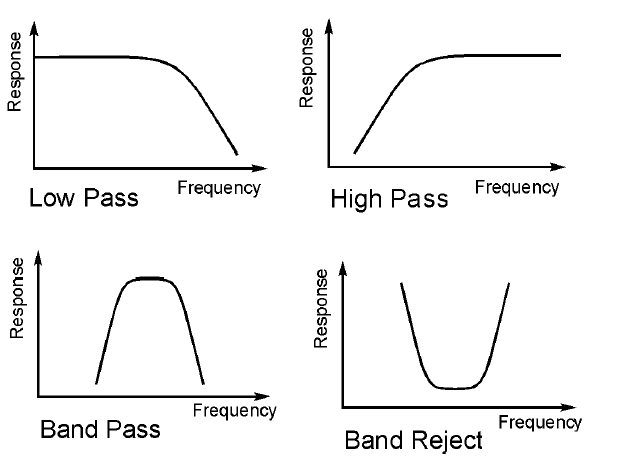
\includegraphics[scale=0.8]{figures/bproblemanalyse/filtertyper.png}
\caption{De fire filtertyper ses her \cite{2. semester kristian}\fxnote{Må man citere til en forelæsning?}}
\label{filtertyper}
\end{figure}

\subsection{Støj}
Støj er den uønskede del af et opsamlet signal, der ikke har nogen relation til det ønskede signal \fxnote{Må man citere til en forelæsning? - Hvis ja, så ved Nikoline, hvilken forelæsning det er}. Signaler, der er fordelt udover et frekvensspektrum, kan filtreres for støj vha. de tidligere beskrevne filtre. \cite{Devasahayam2000}
Støj kan inddeles i flere forskellige generelle typer, som typisk vil forekomme:

\begin{itemize}
\item Elektriske signaler: Dette er bl.a. 50 Hz støj, som er en frekvens fra elnettet. Denne 50 Hz frekvens kan gå ind og påvirke de biologiske signaler, der måles på. Hvis der er flere 50 Hz kilder, der interagerer, kan det give ekko ved eksempelvis 100 Hz og 150 Hz. Det er denne form for støj, der skal undgås, når signalet analyseres.
\item Ledninger: Kan fungere som antenner, der opfanger 50 Hz støj og andre former for støj. Problemet bliver større jo længere ledningen er. 
\item Magnetfelt: Kan komme i kontakt med ledningerne og derved inducere strømmen, der skaber støj i signalet. Jordens magnetfelt kan f.eks. påvirke ledningerne. For at mindske støjen kan ledningerne snoes / flettes sammen.
\end{itemize} 
% !TeX spellcheck = da_DK
\subsection{Komparator}\label{Komparatorafsnit}
En analog komparator er et kredsløb, der sammenligner en inputspænding eller -strøm med en eller flere referencespændinger eller -strømme. Rent teknisk gøres dette ved, at komparatoren inverterer inputsignalet $\pm 180^{\circ} V_{-}$, imens referencesignalet ikke inverteres $(V_{+})$. Hvis inputsignalet passer med en eller flere af referenceværdierne, vil de tilknyttede komponenter aktiveres. Den simpleste komparator er en operationsforstærker uden modkobling. \cite{webster2009} \\
Komparatorens output går fra en mætningsgrænse til en anden, når det negative input af operationsforstærkeren passerer igennem 0 V. Dette betyder, at ved et inputsignal på mere end tærskelniveauet vil outputsignalet opnå negativ mætningsgrad. Omvendt ved et inputsignal, som er lavere end tærskelniveauet, vil outputsignalet opnå positiv mætningsgrad. \cite{webster2009} 

%Det kan være fordelagtig at placere modstanden R1 ved inputsignalet, som det kan ses på \figref{komparator}, da dette minimerer overstyringen\fxnote{Et bedre ord end overstyring} af operationsforstærkeren.  Når inputtet, ved en simpel komparator, når tærskelniveauet og der forekommer støj på inputtet, kan outputsignalet svinge kraftigt. Dette kan imidlertid undgås ved at tilføje to modstande, R2 og R3. \cite{webster2009}

% !TeX spellcheck = da_DK
\subsection{ADC og konvertering til computeren}
Når der foretages målinger på kroppens signaler er output et analogt signal, som er kontinuert i tid og amplitude. Ved behandling af det analoge signal anvendes digital processering, hvilket betyder, at det analoge signal skal konverteres til et digital signal vha. en ADV (Analog-to-Digital-Converter). Det digitale signal er diskret i tid og amplitude, så det analoge signal kvantificeres under konverteringen \cite{Webster2009}. Konverteringsprocessen består af to dele, som er sampling og kvantisering \cite{Zouridakis2003}.  

Sampling er processen, hvor diskretisering i tidsdomænet finder sted, dvs. tidsdomænet i det kontinuerte signal konverteres til et diskret signal. Samplingsfrekvensen er den hyppighed hvormed signalet måles og hvis der ikke vælges en passende samplingsfrekvens, kan information fra det originale signal gå tabt. Ifølge Nyquists teorem er en hensigtsmæssig samplingsfrekvens således, at samplingsfrekvensen skal være mindst det dobbelte af frekvensen i det originale signal. \cite{Zouridakis2003} Det anbefales dog i praksis at sample med en samplingsfrekvens, der er ti gange frekvensen af det originale signal \fx{kilde??}. En for lav samplingsrate kan medføre, at kurven fra det rekonstruerede signal ligger forskudt ift. det originale signal, hvilket kaldes alias. \cite{Zouridakis2003}
 
Diskretisering af amplituden betegnes som kvantisering. De enkelte samples har en amplitudeværdi og ved kvantisering inddeles denne analoge værdi i trin. I modsætning til samling sker der en approksimering i det rekonstruerede signal, da værdierne mellem to trin repræsenteres af samme digitale værdi. \cite{Zouridakis2003} Antallet af amplitudeniveauer, der er tilgængelige til at repræsentere det analoge signal, determineres af antal bits. F.eks. en ADC med en opløsning på 12-bit inddeles i 4096 niveauer, da $2^12$=4096. \cite{Konrad2006} Det mindste amplitudeniveau ADC'en kan opnå kaldes LSB (Least Significant Bit) og bestemmes ved følgende ligning \fxnote{kilde?? - mine noter}: $LSB = \frac{FSR}{(2n-1)} = \frac{FSR}/{2^n}$, hvor FSR er "full scale voltage range" (arbejdsområdet), n er antal bits, $2^n$ er antal værdier og $2^n$-1 er antal intervaller. 

Ved forstærkning er det essentielt at være opmærksom på ADC'ens \fxnote{kan man skrive det?} arbejdsområde. F.eks. hvis signalet er højere eller mindre end ADC'ens arbejdsområde, vil signalet blive klippet. \fxnote{problemer igen med at finde nogle kilder til det} 
 
\clearpage
% !TeX spellcheck = da_DK
\section{Problemafgrænsning}
Apopleksi er en sygdom, der har stor indflydelse på blodtilførslen til encephalon. Hvis tilstrømningen af blod er nedsat, kan der opstå både motoriske og sensoriske skader hos patienten, hvilket kan komme til udtryk som balanceproblemer. Balancen er vigtig for at kunne fungere i dagligdagen, da den sikrer at man holder kroppen oprejst og muliggør bevægelse uden fald. \cite{Nichols1997} Apopleksipatienter med balanceproblemer oplever en begrænsning i deres dagligdag, da de er afhængige af hjælp til daglige gøremål, som de før sygdommen selv kunne udføre. De oplever det som et brud på deres tidligere liv, hvilket påvirker deres identitet og livskvalitet. \cite{Sundhedsstyrelsen2010}

For at begrænse de fysiske, og dermed også de personlige, følger mest muligt, er det essentielt at rehabiliteringen påbegyndes hurtigt efter apopleksitilfældet. Rehabilitering omfatter både genoptræning af fysiske funktioner, herunder balancefunktionen, men også tilpasning til miljø og styrkelse af sociale kompetencer.\fxnote{Ingen kilde på dette i afsnittet..} Indenfor rehabilitering af balance tilbydes forskellige metoder, såsom... \fxnote{ex. 2 metoder fra nuværende metoder} En anden mulighed ift. rehabilitering af balancen er biofeedback. Studier viser positive resultater med biomekanisk biofeedback, hvor der måles på kroppens generelle motoriske egenskaber. \cite{Giggins2013} For at biofeedback er en mulighed, er det en forudsætning, at patientens kognitive evner er tilstrækkelige til at kunne blive instrueret og kunne huske de indlærte øvelser fra gang til gang. Derudover er der visse krav til de neurologiske og motoriske evner \fxnote{de krav de opstiller i afsnit om biofeedback til patienten kan komme ind her, så det bliver mere specifikt}. \cite{Middaugh1989}

Det er derfor interessant at undersøge, hvordan der kan udvikles et system baseret på biofeedback, der kan hjælpe patienter med at genoptræne deres balance. Det er relevant at undersøge, om der kan designes et system, som i højere grad tillader patienterne at bidrage til deres egen rehabilitering. Det er muligt, at dette kan begrænse nogle af patienternes personlige følger, da kontakten med sundhedspersonale i forbindelse med rehabiliteringen evt. kan begrænses, hvormed det normale hverdagsliv hurtigere kan genoptages. \fxnote{Jeg her mest bare forkortet problemafgrænsningen, så der skal muligvis tilføjes enkelte linjer, som der er blevet skrevet til efter Erikas rettelser for at spore os helt ind på problemet}

\section{Problemformulering}
Hvordan designes et biofeedback system således, at det hjælper apopleksipatienter under rehabilitering af balancen?


%Apopleksi er den tredje største dødsårsag i Danmark \cite{Hjernesagen2015a}. 
%Af alle tilfælde af apopleksi er den iskæmiske langt den hyppigste med 80-85\% af tilfældene, imens den hæmoragiske udgør 10-15\%.
%Sygdommen har stor indvirkning på blodtilførslen til encephalon, som er det område af hjernen, der bla. rummer cerebrum. I cerebrum sker behandlingen af bla. sensoriske signaler, tanker og følelser. Når blodtilførslen til encephalon, og dermed også cerebrum, er nedsat, vil der kunne opstå både motoriske og sensoriske skader hos patienten.
%Når en patient med formodet apopleksi bliver indlagt, er det vigtigt, at lægen laver en grundig undersøgelse af de sensoriske og motoriske evner. Herefter foretages videre undersøgelser, eksempelvis CT- eller MR-scanning, afhængigt af den givne situation. \cite{Sundhedsstyrelsen2009} Det er vigtigt, at behandlingen igangsættes hurtigst muligt for at begrænse følgevirkningerne\cite{Soenderborg2013}. Der findes flere forskellige behandlingsmetoder. Ved iskæmi foregår behandlingen f.eks. med blodfortyndende medicin, en såkaldt trombolysebehandling, der har til formål at opløse blodproppen \cite{Hjernesagen2015b}. \fxnote{Mangler vi ikke noget om behandlingen af hæmoragi??}
%Apopleksi kan medføre sensoriske og motoriske skader. Disse skader kan have stor indvirkning på patientens liv efter sygdomsforløbet og en række psykiske konsekvenser og nedsat livskvalitet, bla. pga. sygdommens pludselige opståen. \cite{Muus2008}
%To eksempler på følger er balanceproblemer og neglekt. Balancen er vigtig for at kunne fungere i dagligdagen, da den sikrer at man holder kroppen oprejst og muliggør bevægelse uden fald. \cite{Nichols1997} Apopleksipatienter kan f.eks. lide af "Pusher Syndrom", hvor de ubevidst læner sig væk fra deres raske side. Dette påvirker balancen og kan lede til ulykker. \cite{Karnath2003} Ved neglekt er patienten ikke bevidst om den ene kropshalvdel. Dette kan være enten et visuelt eller et kropsligt problem. \cite{Sundhed.dk}
%Fælles for de to typer af følger er, at de begrænser patienterne i deres dagligdag og gør dem afhængige af hjælp til mange ting, som de før sygdommen selv kunne udføre. Derfor opleves ofte alvorlige personlige følger, eksempelvis problemer med at opretholde personlige relationer. Derudover kan patienternes identitet og humør også påvirkes. \cite{Sundhedsstyrelsen2010}
%For at begrænse de fysiske - og dermed også de personlige - følger mest muligt, er det essentielt at rehabiliteringen påbegyndes hurtigt efter apopleksien. Rehabiliteringen omfatter både genoptræning af fysiske funktioner, men også tilpasning til miljø og styrkelse af sociale kompetencer.\fxnote{Ingen kilde på dette i afsnittet..} 
%I Danmark er rehabiliteringen organiseret således, at de forskellige aktører i sundhedssektoren arbejder sammen på tværs af hinanden. Dette tværfaglige samarbejde er vigtigt, da apopleksipatienterne er i kontakt med mange forskellige dele af systemet under deres sygdomsforløb. \cite{Sundhedsstyrelsen2010} 
%Der findes i dag flere forskellige metoder til rehabilitering, afhængig af hvilken type følger patienten er ramt af. Metoderne er baseret på forskellige principper, herunder bla. træning vha. lyd, mekanisk træning, spejling og sensorisk stimulation\cite{Bradt2010,Mehrholz2013,Thieme2012,Sundhedsstyrelsen2010}.
%En anden måde at rehabilitere på er vha. biofeedback. Ved biofeedback måles på biologiske signaler, der relaterer til det område eller den funktion, som skal rehabiliteres hos patienten. Disse data omsættes til et signal, der kan opfattes af patienten. \cite{Giggins2013} Der skelnes mellem fysiologisk- og biomekanisk biofeedback\cite{Giggins2013}. Ved fysiologisk biofeedback måles der på kroppens systemer, herunder muskelaktivitet, hjerterytme og respiration. Ved biomekanisk biofeedback måles der på kroppens generelle motoriske egenskaber, eksempelvis hvordan kroppen bevæger sig. Studier har generelt vist positive resultater for biomekanisk biofeedback ift. rehabilitering af balanceproblemer. \cite{Giggins2013}
%For at biofeedback er en mulighed, er det en forudsætning, at patientens kognitive evner er tilstrækkelige til at kunne blive instrueret og kunne huske de indlærte øvelser fra gang til gang. Derudover er der visse krav til de neurologiske og motoriske evner. \cite{Middaugh1989}

%Både når der ses på de samfundsmæssige og personlige omkostninger, er apopleksi en krævende sygdom. Dels fordi sygdomsforløbet foregår i flere forskellige dele af sundhedssystemet og er den sygdom, der kræver flest plejedøgn. Derudover medfører sygdommen alvorlige fysiologiske og mentale følger.

%Det er derfor interessant at undersøge hvordan der kan udvikles et system baseret på biofeedback, der kan hjælpe patienter med at genoptræne deres balance. Det er relevant at undersøge om der kan designes et system, som i højere grad tillader patienterne at bidrage til deres egen rehabilitering. Det er muligt, at dette kan begrænse nogle af patienternes personlige følger, da kontakten med sundhedspersonale i forbindelse med rehabiliteringen evt. kan begrænses, hvormed det normale hverdagsliv hurtigere kan genoptages. 

%Man kan derfor undersøge muligheden for at begrænse både de samfundsmæssige og personlige omkostninger for patienter med balanceproblemer vha. et system baseret på biofeedback. Hvis der kan udvikles et system, der i højere grad tillader patienten at genoptræne sin balance selv, ved at gøre vedkommende opmærksom på eventuel hældning til siden, vil dette muligvis kunne begrænse patientens behov for at være i kontakt med sundhedspersonale, hvormed en normal dagligdag også hurtigere kan påbegyndes igen.  

\chapter{Problemløsning}
% !TeX spellcheck = da_DK
\section{Systembeskrivelse}  

\subsection{Formål og anvendelse}
Systemet har til formål at gøre apopleksipatienter opmærksomme på, hvornår de mister balancen \fxnote{reference til problemafgrænsningen}. Systemet skal derfor kunne registrere, hvis patienten er i risiko for at falde og derved udsende et signal så patienterne har mulighed for at rette sig op igen. Selve systemet skal anvendes så patienterne er mere selvstændige i rehabiliteringsprocessen med henblik på at opnå en bedre balance. 

Det er på baggrund af afsnit.. valgt at hældningen på patienten skal opfanges via en sensor som er placeret på patienten. Systemet skal give visuelt feedback i form af to dioder, når patienten hælder til enten højre eller venstre. Når patienten hælder XX til den ene side indikeres det af en gul diode, hvis patienten hælder yderligere, hvilket svarer til en hældning på XX lyser en rød diode. Derudover anvendes sensorisk feedback via vibration som advarer patienten ved den gule diode og stiger i takt med at patienten hælder mere og mere.  
%Ud fra problemanalysen fremgår det, at ældre over 65 år i højere grad får apopleksi, hvortil balanceproblemer er en hyppig gene. Derudover har apopleksipatienter ofte kognitive problemer. Apopleksipatienter har et ønske om at være selvstændige og uafhængige. 

%Systemet skal opfange, hvis patienten er ude af balance og være nemt anvendeligt, da det skal bruges til selvtræning af balancen i hjemmet - altså implementeres i fase 4, som bliver omtalt på side \pageref{Faser}. For at systemet kan anvendes af målgruppen, skal det være brugervenligt - dvs. let at påsætte, ikke veje for meget samt signalerne skal være let forståelige. Målgruppen giver yderligere begrænsninger ift. feedback, da både hørelsen, synet eller kroppens følelser kan være svækket. Derudover skal systemet kunne give et digitalt output, som er muligt at behandle.

\subsection{Systemets brugere}
Systemet udvikles med henblik på selvtræning af balance i rehabiliteringsfasen. Derfor er systemets primære bruger patienten selv. Jævnfør afsnit (med apopleksipatienters alder) ses det at majoriteten af apopleksipatienter er over 65 år. Systemet skal være let anvendeligt så det kan anvendes af denne ældre demografi. Fagkyndigt personale, såsom fysioterapeuter og læger, skal kunne følge med i udviklingen som patienten gennemgår. Det skal derfor være muligt for disse også at benytte systemet. Dette gøres ved at systemet både har et analogt og digitalt output. Hvor det digitale henvender sig mere til et fagkyndigt personale.

\subsection{Anvendelse}
Systemet designes til at patienten under anvendelsen skal være stående på en tegnet linje med den ene fods tæer mod den anden fods hæl\fxnote{måske et billede vi tager som vil illustrere dette}. Denne position er valgt for at udfordre patientens balance ved at fordele kropsvægten anderledes ift. den normale kropsstilling omtalt på side \pageref{BalanceAfsnit}. Patienten påsætter selv systemet øverst på sternum og udfører herefter en kort prøvetest for at kende til de givne feedbackparametre. Under prøvetesten svajer patienten langsomt fra side til side. Hvis vedkommende hælder over xx grader, vil en gul diode lyse og vibrationen vil begynde. Hvis patienten svajer yderligere og hælder med over xx grader vil en rød diode lyse. Vibrationen vil styrkes i takt med overgangen fra den gule til den røde diode. Efter testøvelsen udføres selve træningsøvelsen. Her indtages udgangspositionen på linjen og øjnene lukkes. Dette gøres for at udelukke den visuelle sans, hvilket gør det sværere for patienten at opretholde balancen. Patienten skal forsøge at holde balancen så længe som muligt uden at bevæge sig ud i risikozonerne, der vil blive markeret ved vibration. Træningsøvelsen gentages efter behov. \\
Ved at tage flere målinger igennem rehabiliteringsforløbet vil det forventes at der sker en fremgang ift. tiden hvori balancen kan opretholdes uden at patienten bevæge sig ud i risikozonerne. 

\subsection{Optagelse af signal fra accelerometer}
Acceleorometeret skal give et elektrisk signal ud fra den position som anvendes i forsøget \fxnote{Vi skal vurdere hvor signalet kommer fra om det x,y,z aksen.}. Accelerometeret opfanger de signaler som udsendes fra sensoren som er placeret anteriort på patientens brystkasse. Signalet afhænger af, hvor langt patienten har flyttet sig. 

............ HER MANGLER NOGET INFORMATION..........................

Ledningerne snoes for at kontrollere samt mindske støjen. Derudover sættes ledninger fast med tape på patienten, så vidt det er muligt. For at undgå unødvendigt støj foretages forsøget væk fra andet elektronik.  %\ref{reference til støj afsnittet}



\subsection{Analogt output}
Det analoge output skal kunne henvende sig til patienten, dette sker ved lysdioder og vibration. Lysdioderne skal lyse gult ved 'usikkerhed' og slukke hvis patienten enten er rettet op igen eller bevæger sig ud i riskozonen, hvorefter en ny diode skal lyse rødt. Vibrationerne igangsættes ved 'usikkerhed' og skal stoppe hvis patienten retter sig op eller stige i styrke, hvis patienten kommer ud i risikozonen. 

\subsection{Digitalt output}
Det digitale skal kunne anvendes af sundhedspersonale til at vurdere om patienten gør fremskridt, dette indebærer at informationerne for patienten kan gemmes og sammenlignes på en computer. 


\subsection{Systemets opbygning}
Systemets opbygning fremgår af \figref{kravblok}.

\begin{figure}[H]
	\centering
	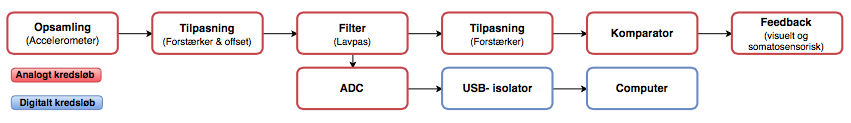
\includegraphics[scale=0.62]{figures/cProblemloesning/blokdiagram1.png}
	\caption{Figuren viser de blokke/elementer som systemet skal indeholde}
	\label{kravblok}
\end{figure}

Signalerne fra accelerometeret skal forstrækes, herefter støj skal filteres fra for at dæmpe uønskede frekvenser. Herefter forstærkes signalet med en variabel forstærkningen, da signalet kun er forstærket lidt. Signalet forstærkes til maksimalt 3V. Dette gøres ved en operationsforstærker \fxnote{inverteret eller ikke-inverteret} Det analoge signal ensrettet via. \fxnote{helbølgeensretter eller halvbølgeensretter}, hvor efter der benyttes en integrator til at lave en lineær linje. Ud fra denne linje gives en advarsel via feedback. Det digitale signal skal konverteres fra analogt til digitalt, hvilket gøres ved en ADC.  Herefter anvendes en USB-isolator for patientsikkerhed. Computeren skal fremvise en graf når NIDAQ er tilsluttet. 

\subsection{Kravspecifikationer}
Til vurdering af tolerance er der udført et pilotforsøg, dette er udført med henblik på at kunne beregne forstærkning, filtrering og integrering af signalet. 

\subsubsection{Det samlede system}
Det analoge output sammenligninger inputtet som kommer fra accelerometeret og outputtet i form af 2 dioder og stigning i vibration. Aktivering af bestemte dioder skal afspejle inputsignalet således at et lille input aktiverer en gul diode og vibration, mens et større input aktiverer en rød diode og stigningen i vibration. 

\textbf{Krav:}
\begin{itemize}
\item Den gule diode skal lyse når patienten har bevæget sig XX og slukke hvis patienten retter sig op eller hælder yderligere.
\item Den røde diode skal lyse når patienten har bevæget sig XX og slukke, hvis patienten retter sig op.
\item Vibration skal igangsættes når patienten har bevæget sig XX og skal slukke, hvis patienten retter sig op eller stige, hvis patienten hælder yderligere.
\item Der skal være en sammenhæng mellem inputsignalets størrelse og antallet af dioder der lyser?
\item Signalet i systemet må ikke forstærkes til en værdi over 3V.
\end{itemize}

\subsection{Krav}
For at gøre anvendelse af samme system muligt til 4. Semester skal arbejdsområdet kunne benyttes sammen med et USB-baseret trådløst udviklingsværktøj eZ430-RF2500 fra Texas Instruments. Det er derfor nødvendigt, at designet stemmer overens med udviklingsværktøjet for at kunne sende og modtage data til og fra computeren. Udviklingsværktøjet indeholder hardware og software som evaluerer mikrokontrolleren MSP430F2274. For at hele vores system kan anvendes med udviklingsværktøjet, skal outputsignalet være 3V, eftersom mikrokontrolleren opererer med spændingsforsyning mellem 1,8V og 3,6V.

%\textbf{Tolerance:}
%\begin{itemize}
%\end{itemize}
%
%\subsubsection{Accelerometer}
%\textbf{Krav:}
%\begin{itemize}
%\end{itemize}
%
%\textbf{Tolerance:}
%\begin{itemize}
%end{itemize}
%
%\subsubsection{Instrumentering forstærker}
%\textbf{Krav:}
%\begin{itemize}
%\end{itemize}
%
%\textbf{Tolerance:}
%\begin{itemize}
%\end{itemize}
%
%\subsubsection{Filtre - opdeling i høj og lavpass?}
%\textbf{Krav:}
%\begin{itemize}
%\end{itemize}
%
%\textbf{Tolerance:}
%\begin{itemize}
%\end{itemize}

%\subsubsection{Forstærker med variabel forstærkning}

%\textbf{Krav:}
%\begin{itemize}
%\end{itemize}
%
%\textbf{Tolerance:}
%\begin{itemize}
%\end{itemize}
%
%\subsubsection{Ensretter}

%\textbf{Krav:}
%\begin{itemize}
%\end{itemize}
%
%\textbf{Tolerance:}
%begin{itemize}
%end{itemize}
%
%\subsubsection{Integrator}
%\textbf{Krav:}
%\begin{itemize}
%\end{itemize}
%
%\textbf{Tolerance:}
%\begin{itemize}
%\end{itemize}
%
%\subsubsection{Advarsel}
%\textbf{Krav:}
%\begin{itemize}
%\end{itemize}
%
%\textbf{Tolerance:}
%\begin{itemize}
%\end{itemize}
%
%\subsubsection{ADC}
%\textbf{Krav:}
%\begin{itemize}
%\end{itemize}
%
%\textbf{Tolerance:}
%\begin{itemize}
%\end{itemize}
%
%\subsubsection{USB-isolator}
%\textbf{Krav:}
%\begin{itemize}
%\end{itemize}
%
%\textbf{Tolerance:}
%\begin{itemize}
%\end{itemize}
%
%\subsubsection{Computer}
%\textbf{Krav:}
%\begin{itemize}
%\end{itemize}
%
%\textbf{Tolerance:}
%\begin{itemize}
%\end{itemize}
%\begin{itemize}
%\item Systemet skal ved fald få dioder til at lyse samt give feedback i form af stigende vibration. 
%\item Systemet skal være non-invasiv - dvs. systemet ikke må påføre patienten smerte eller varig skade
%\item Systemet skal være brugervenligt
%\item Systemet skal forsynes med spænding fra 9V batteri
%\end{itemize}

%\subsubsection{Accelerometer}
%Accelerometeret skal detektere patientens kropshældning.

%\subsubsection{Filter}
%Når der anvendes et filter, skal det dæmpe uønskede frekvenser. Dvs. frekvenser der lavere eller højere ift. det signal fra accelerometeret, som man vil analysere på. Der skal udføres et pilotforsøg for at finde frem til det korrekte filter og valg af knækfrekvens. 

%\subsubsection{Signalerende lys}
%Når patienten er ude af balance skal en rød diode lyse, som signalering ift. patientens hældning. Der skal vha. et pilotforsøg detekteres, hvornår dioden skal lyse. Skal der evt. være 2 dioder, hvor den ene er et "advarende" signal og nr. to er "fare". 

%\subsubsection{Alarm/vibrationen}
%Alarmen/vibrationen skal anvendes i perioden, hvor patienten er ude af balance og stoppe igen, når der igen er oprettet balance. 
%(eller fungere som en alarm til dioderne - så når en diode lyser, skal alarmen gå)

%\subsubsection{ADC}
%Der anvendes en ADC i systemet, for at konvertere det analoge signal til digitalt. Det næste skridt er konverteringen til PC og det er derfor essentielt at have en ADC, der konverterer analogt signal til binære tal, som digitale systemet anvender. 
%{Her skal vi have valgt en samplingsfrekvens)

%\subsubsection{USB-isolater}
%USB-isolatoren sikre patientens sikkerhed. Her skal input- og outputspænding være ens.  

%\subsubsection{Til PC}
%Fremvisning af graf, så patienten og plejepersonale kan følge %rehabiliteringens udvikling. 

% !TeX spellcheck = da_DK
\section{Pilotforsøg}\label{Sec:PilotforsoegKort}
Der udføres i dette projekt et pilotforsøg for at identificere og sammenligne væsentlige parametre ift. det anvendte accelerometer. En udførlig beskrivelse af pilotforsøget kan ses i bilag \ref{Bilag:Pilotforsoeg} på side \pageref{Bilag:Pilotforsoeg}.
Formålet med pilotforsøget er at kunne fastsætte det frekvensspektrum, som det ønskede signal ligger indenfor, da det på den måde er muligt at frafiltrere støjsignaler fra det opsamlede signal. Derudover skal det maksimale og minimale outputsignal fra accelerometeret identificeres, for at spændingsværdierne for de valgte hældningsgrader kan udregnes. Pilotforsøget udføres desuden for at sammenligne de målte offset- og sensitivitetsværdier med de oplyste værdier i databladet for accelerometeret. 
\subsection{Konklusion}
På baggrund af målinger og beregninger i pilotforsøget kan det konkluderes, at for outputsignalet fra accelerometret ved den statiske acceleration udgør alt over $0Hz$ støj. Der udregnes en baseline ved $0$g påvirkning til $1.6325$V, som burde være $1.65$V, da dette er halvdelen af spændingsforsyningen. Derved afviger den målte baseline med $1.06$\%. Ved rotationsmålingerne vurderes det, at alt over $25$Hz er støj. Maksimum og minimum outputsignalet fra accelerometret vil for langsom rotation eller svajning henholdsvis være $1.9638$V og $1.3092$V, hvilket bliver til $0.3313$V og -$0.3233$V efter offsettet er blevet justeret, der udregnes til $0.0037$V og -$0.0036$V pr grad. Afvigelserne mellem pilotforsøg og datablad vurderes som værende acceptable ift. videre udførelse af forsøg med accelerometeret. 


% !TeX spellcheck = da_DK
\section{Specifikke kravspecifikationer}
I praksis er det ikke muligt at have ideelle komponenter \cite{Nilsson2011}. Der vurderes derfor ud fra pilotforsøget, litteratur samt relevante datablade, hvilke krav blokkene i blokdiagrammet i afsnit \ref{kravblok} på side \pageref{kravblok} skal opfylde og den tolerance, der accepteres ift. forskellige parametre.

\subsection{Opsamling}\label{OpsamlingsAfs}
Blokken opsamling omfatter accelerometeret, offsetjustering og forstærkning. Accelerometeret skal have en sådan størrelse, at det kan påsættes en patient uden at give fysiske begrænsninger. Accelerometeret skal kunne måle en statisk acceleration i mindst to retninger, da der måles i det frontale plan til hhv. højre og venstre side. Herved kan det bestemmes, hvilken retning patienterne hælder mod i stående position. Det skal kunne detektere en hældningsgrad op til $\pm90^{\circ}$, da en forsøgsperson ikke kan komme over denne hældningsgrad. \\
Offsetjusteringen skal centrere det målte signal omkring $0V$, da accelerometeret typisk måler $1.6325V$ ved $0$g påvirkning af den pågældende akse ifølge pilotforsøget. Derfor skal der trækkes $1.6325$V fra alle inputs fra accelerometret. Justeringen af offset skal forekomme inden forstærkning således, at der ikke sker en forstærkning og dermed forskydning af offsetværdien, når accelerometret måler i positiv og negativ retning, hvorved g påvirkningen ændres. Ved justering af offsettet må der ikke ske en ændring af amplitudens peak-to-peak og frekvensen. \\
Forstærkningen skal gøre det nemmere at adskille det ønskede signal fra støj i den efterfølgende filtreringsblok. For at forstærkningskredsløbet ikke dræner strømforsyningen, skal inputimpedansen til forstærkeren være mindst $100$ gange større end outputimpedansen i accelerometeret som kan ses i afsnit \ref{Subsec:AccTeori} på side \pageref{Subsec:AccTeori}. Signalet skal efter forstærkningen ligge indenfor arbejdsområdet $\pm3V$ og der ønskes derfor størst mulige forstærkning. Den højeste måling ved $\pm90^{\circ}$ var ifølge pilotforsøget efter offsetjusteringen $0.3313$V. Derfor kan forstærkningen udregnes således:
\begin{equation}
\dfrac{3\text{V}}{0.3313\text{V}} =  9.05 \approx 9.1
\end{equation}
\noindent Der ønskes en forstærkning på faktor $9.1$. Derved vil den maksimale spænding efter denne forstærkning være $3.0148$V, hvilket accepteres, da der vides fra databladet for operationsforstærkeren TL081 og teori, at når TL081 bliver forsynet med en spænding på $5.5$V, så vil den maks give ca. $4$V ud. \cite{Corporation1995} Derfor vil en lille afvigelse i outputsignalet ift. arbejdsområdet ikke få systemet til at gå i mætning. Forstærkningens gain i dB udregnes ud fra følgende formel: 
\begin{equation}
20 \cdot log_{10} (9.1) = 19.1808\text{dB}
\end{equation} 

\noindent\textbf{Krav:}
\begin{itemize}
	\item Opsamlingsblokken skal have en spændingsforsyning på $5.5$V.
	\item Accelerometeret skal minimum have en output akse.%, da der udelukkende måles i det frontale plan.
	\item Accelerometeret skal være under $5x5$ cm i dimensionerne.%, da dette gør implementeringen på patienten nemmere.
	\item Accelerometeret skal kunne måle statisk acceleration i mindst to retninger.
	\item Accelerometeret skal kunne detektere en hældning fra $0^{\circ}$ til $\pm90^{\circ}$.
	\item Offsetjusteringen skal centrere det målte signal omkring $0V$.
	\item Offsetjusteringen skal modtage en referencespænding på $1.6325$V.
	\item Forstærkeren skal have en indgangsimpedans på mindst $3.68M\Omega$\fxnote{Da man ikke vil dræne blokken før for strøm. Udregnet ved $32K\Omega$, da indputimpedans skal være mindst $100$ gange større end den forrige bloks outputimpedans. Accelerometrets indgangsimpedans har en afvigelse på +$15$\%}.
	\item Forstærkningen skal være på $9.1$, som svarer til $19.1808$dB.
	\item De benyttede modstande til designet af forstærkeren skal besidde den navngivne værdi.
	\item Outputtet fra denne blok skal være mellem $2.9817$V og -$2.9097$V.
\end{itemize}
\textbf{Tolerance:}
\begin{itemize}
	\item Der accepteres en afvigelse i spændingsforsyning på $\pm9\%$.
	\item Der accepteres ingen afvigelse ift. krav for accelerometerets dimension og minimum antal af akser.
	\item Der accepteres en afvigelse i detektionen af hældningsgrad på $\pm5\%$.
	\item Der accepteres en afvigelse af offsetjusteringen på $\pm2\%$.
	\item Der accepteres en afvigelse i referencespændingen på $\pm0.003$V.
	\item Der accepteres kun en indgangsimpedans i forstærkeren på mindst $3.68M\Omega$.
	\item Der accepteres en afvigelse i forstærkningen på $\pm2\%$.
	\item Der accepteres en afvigelse i de benyttede modstandes reelle værdi på $\pm1\%$.
	\item Der accepteres en afvigelse ift. maksimum og minimum output fra blokken på $\pm5\%$.
\end{itemize}
%%%%%%%%%%%%%%%%%%%%%%%%%%%%%%%%%%%%%%%%%%%%%%%%%%%%%%%%%%%%%%%%%%%%%
\subsection{Filter}\label{FilterAfs}
Blokken indeholdende et filter anvendes til at frasortere uønskede signaler, der kan forekomme under målinger med accelerometret. Filtreringsblokken inddrages i systemet jævnfør afsnit\ref{Filterafsnit} på side \pageref{Filterafsnit}. Frekvensområdet for kropshældning er ikke klart defineret, men studier anvender et frekvensområde liggende mellem $0.02-10Hz$ \cite{Martinez-Mendez2011}. Alle signaler, der ligger udenfor dette spektrum, ønskes derfor fjernet. I pilotforsøget blev der påvist, at signalet i dette tilfælde ligger mellem $0-25Hz$. Alt signal uden for dette spektrum ønskes derfor frafiltreret. Dette gøres ved at benytte et lavpasfilter, der har en knækfrekvens ved $25$Hz. \\
Den maksimale variation i pasbåndstransmissionen ($A_{max}$) sættes til $3$dB. For fjerne $50Hz$ støj, sættes stopbåndsfrekvensen til $45$Hz, og der udregnes en faktor ud fra LSB \ref{ADCafsnit} og den maksimale amplitude af signalet. Den maksimale amplitude beregnes ved en Root Mean Square (RMS) analyse ud fra rotationerne foretaget i \ref{Sec:Pilotforsoeg} for hhv. højre og venstre side. Dæmpningsfaktoren udregnes ved følgende ligning:
\begin{equation}
\dfrac{0.00244\text{V}}{0.0162\text{V}} = 0.1506 \approx 0.2 
\end{equation}
\begin{equation}
\dfrac{0.00244\text{V}}{0.0131\text{V}} = 0.1863  \approx 0.2
\end{equation}
Der ønskes en dæmpning på faktor $\dfrac{1}{5}$, da der tages forbehold for et tolerance område. Dæmpningens gain i $dB(A_{min})$ udregnes ud fra følgende formel:   
\begin{equation}
A_{min}=20 \cdot log_{10} \cdot (\frac{1}{5}) = -13,98 \approx -14\text{dB}
\end{equation}
\textbf{Krav:}
\begin{itemize}
	\item Filteret skal have en spændingsforsyning på $5.5$V.
	\item Filteret skal kunne modtage et inputsignal på $\pm3V$.
	\item Der ønskes en knækfrekvens i pasbåndet på $25$Hz.
	\item Der ønskes en stopbåndsfrekvens på $45$Hz.
	\item Der ønskes maksimal fladhed på pasbåndet og stopbåndet.
	\item Der ønskes en minimum dæmpning af stopbåndet på $14$dB.
	\item Der ønskes en maksimal dæmpnning i pasbåndet på $3$dB.
\end{itemize}
\textbf{Tolerance:}
\begin{itemize}
	\item Der accepteres en afvigelse i spændingsforsyning på $\pm9\%$.
	\item Der accepteres ingen afvigelse ift. hvor stort et inputsignal filtret skal kunne modtage.
	\item Der accepteres en afvigelse fra knækfrekvensen på $\pm10\%$.
	\item Der accepteres en afvigelse fra stopbåndsfrekvensen på $\pm5\%$.
	\item Der accepteres kun en maksimal fladhed på pasbåndet og stopbåndet.\item{Hvordan tjekker man, at det man har fået er det maksimale?}
	\item Der accepteres minimal dæmpning på $14$dB af stopbåndet eller en afvigelse på $+15\%$.
	\item Der accepteres maksimal dæmpning på $3$dB af pasbåndet eller en afvigelse på $-15\%$.
\end{itemize}
%%%%%%%%%%%%%%%%%%%%%%%%%%%%%%%%%%%%%%%%%%%%%%%%%%%%%%%%%%%%%%%%%%%
\subsection{Tilpasning}\label{Tilpasningsblok}
Blokken tilpasning har til formål at tilpasse det filtrerede signal til komparatoren. Dette gøres med en forstærker, således at spektret, der skal reguleres indenfor, øges. Derudover afgrænses måleintervallet til $\pm25^{\circ}$, da et range på $\pm90^{\circ}$ er unødvendigt ift. at vurdere hvorvidt patienten er faldet. Det vurderes, at en hældning på over $25^{\circ}$ medfører fald, da denne hældning ligger væsentligt ud over den naturlige hældningsgrad jævnfør afsnit \ref{BalanceAfsnit}, side \pageref{BalanceAfsnit}. Der ønskes størst mulig forstærkning indenfor det fastsatte arbejdsområde på $\pm3$V. Indgangsimpedansen bestemmes ud fra samme kriterier som for forstærkeren i opsamlingsblokken. I bilag \ref{Bilag:Pilotforsoeg} på side \pageref{Bilag:Pilotforsoeg} er den størst mulige spænding efter justering af offsettet udregnet, hvilket er $0.3313V$. Derudover er der det beregnet, at den maksimale volt pr. grad er $0.0037$V. Ved $\pm25^{\circ}$ vil outputtet være;
\begin{align}
\label{Udreg3} 0.0037 \cdot 25 = 0.0925V
\end{align}
Forstærkerens faktor samt gain i dB udregnes i \eqref{TilpasEq2} og \eqref{TilpasEq3}.
\begin{align}
\label{TilpasEq1} 0.0925V \cdot 9.1 = 0.8418V \\
\label{TilpasEq2} \dfrac{3V}{0.8418V} = 3.5638 \approx 3.6 \\
\label{TilpasEq3} 20 \cdot log_{10} (3.6) = 11.1261\text{dB}
\end{align} 
I \eqref{TilpasEq1}, \eqref{TilpasEq2} og \eqref{TilpasEq3} er de $3V$ grænsen for arbejdsområdet. Der forstærkes med en faktor $3.6$. \\

\noindent\textbf{Krav:}
\begin{itemize}
	\item Forstærkeren skal modtage en spændingsforsyning på $5.5$V.
	\item Forstærkeren skal kunne modtage et inputsignal på $\pm3V$.
	\item Forstærkeren skal forstærke med en faktor $3.6$, som svarer til $11.1261dB$.
	\item De benyttede modstande til designet af forstærkeren skal besidde den navngivne værdi.
	\item Indgangsimpedansen skal være over $3.2M\Omega$.
	\item Outputimpedansen skal være under $32K\Omega$.
\end{itemize}
\noindent\textbf{Tolerance:}
\begin{itemize}
	\item Der accepteres en afvigelse i spændingsforsyning på $\pm9\%$.
	\item Der accepteres ingen afvigelse ift. hvor stort et inputsignal forstærkeren skal kunne modtage.
	\item Der accepteres en afvigelse i forstærkningen på $\pm2\%$.
	\item Der accepteres en afvigelse i de benyttede modstandes reelle værdi på $\pm1\%$.
	\item Der accepteres en indgangsimpedans på mindst $3.2M\Omega$.
	\item Der accepteres en outputimpedans under $32K\Omega$.
\end{itemize}
%%%%%%%%%%%%%%%%%%%%%%%%%%%%%%%%%%%%%%%%%%%%%%%%%%%%%%%%%%%%%%%%%%%%%
\subsection{Komparator}\label{KomparatorAfs} 
Blokken indeholdende komparatorer skal kunne sammenligne inputsignalet med referencespændinger og kunne modtage et signal mellem $\pm3$V. Komparatorerne skal vha. definerede tærskelværdier bestemme hvilken hældningsgrad patienten har og i hvilken retning vedkommende hælder mod. Der skal være flere tærskelværdier, så feedbacken kan gives i flere niveauer og forskellige sværhedsgrader. Dette gør systemet fleksibelt, så det kan benyttes af patienter på forskellige balanceniveauer. Tærskelværdierne er bestemt på baggrund af pilotforsøg, hvor værdierne er beregnet ved først at finde spændingen for $90^{\circ}$, som jævnført \ref{Sec:Pilotforsoeg} på side \pageref{Sec:Pilotforsoeg} er $0.3313$V for positiv retning og -$0.3233$V i negativ retning efter forstærkning på hhv. en faktor $9.1$ og derefter en faktor $3.6$. Denne værdi divideres med $90$ for at bestemme spændingen ved $\pm1^{\circ}$ og ganges herefter med hhv. $2^{\circ}$,  $8^{\circ}$, $13^{\circ}$ og $25^{\circ}$ for at bestemme spændingen ved de enkelte hældninger.\\
\textbf{Krav:} 
\begin{itemize}
	\item Komparatorblokken skal have en spændingsforsyningen på $\pm5.5$V.
	\item Komparatoren skal kunne skifte mellem to sværhedsgrader ved at ændre tærskelværdierne.
	\item Komparatoren skal kunne modtage et inputsignal på $\pm3$V. 
	\item Komparatoren skal ved et bestemt spændingsniveauer aktivere en diode og vibrator:
	\begin{itemize}
		\item Grøn diode og ingen vibration: I intervallet indenfor $0.1808$V til -$0.1773$V. Svarende til $\pm2^{\circ}$.
		\item Gul diode og let vibration: Fra niveauet $0.9648$V og -$0.9413$V. Svarende til $\pm 8^{\circ}$ eller over.
		\item Rød diode og moderat vibration: Fra nivauet $1.5679$V og -$1.5297$V. Svarende til $\pm13^{\circ}$ eller over.
		%\item Ingen feedback: Over $2.2602$V og under -$2.2168$V. 
	\end{itemize}
\end{itemize}
\textbf{Tolerance:}
\begin{itemize}
	\item Der accepteres en afvigelse i spændingsforsyningen på $\pm5\%$.
	\item Der accepteres ikke, at komparatoren ikke kan skifte imellem to sværhedsgrader.
	\item Der accepteres ingen afvigelse ift. hvor stort et inputsignal komparatoren skal kunne modtage.
	\item Der accepteres en afvigelse i tærskelværdien på $\pm1\%$.
\end{itemize}
%%%%%%%%%%%%%%%%%%%%%%%%%%%%%%%%%%%%%%%%%%%%%%%%%%%%%%%%%%%%%%%%%%%%%%
\subsection{Visuel feedback}\label{visuel_feedback_krav}
Blokken med visuel feedback omfatter den del af systemet, der giver feedback til patienten vha. LED-dioder. Der skal i alt være fem LED-dioder: En grøn, der placeres i midten, en gul på hver side af den grønne diode og en rød diode på hver side af de gule dioder. Den grønne LED-diode skal lyse, når accelerometret er placeret korrekt på patienten, hvorved der er sikret den rette udgangsposition for hældningen. Dette gør, at den grønne LED-diode er aktiveret fra $0^{\circ}$-$2^{\circ}$. I intervallet $2^{\circ}$-$8^{\circ}$ lyser ingen LED-dioder. Den gule LED-diode aktiveres, når patienten skal være opmærksom på sin kropshældning ved en hældning på $8^{\circ}$. Den røde LED-diode aktiveres, når patienten er over $13^{\circ}$ og derfor er i fare for at falde. Retningen af patientens kropshældning bestemmes vha. placeringen af LED-dioderne. LED-dioderne til højre for den grønne LED-diode indikerer at patienten er ved at falde til højre. Det samme gør sig gældende for fald til venstre. 
\\
\textbf{Krav:}
\begin{itemize}
	\item Den visuelle feedbackblok skal have en spændingsforsyning på  $5.5$V.
	\item LED-dioderne skal aktiveres ved angivet spændingsniveauer i komparatoren.
	%\item LED-dioderne skal informere patienten om hvilken retning kropshældningen sker i.
	%\item LED-dioderne skal kunne informere patienten omkring accelerometerets placering.
	%\item LED-dioderne skal informere patienten om risikoen for fald.
	\item LED-dioderne skal kunne give et tydeligt lys.
\end{itemize}
\textbf{Tolerance:}
\begin{itemize}
	\item Der accepteres en afvigelse i spændingsforsyningen på $\pm5\%$.
	\item Der accepteres ingen afvigelse ift. aktivering af LED-dioder ved angivet spændingsniveauer i komparatoren.
	\item Der accepteres kun tydeligt lys fra LED-dioderne.
\end{itemize}
%%%%%%%%%%%%%%%%%%%%%%%%%%%%%%%%%%%%%%%%%%%%%%%%%%%%%%%%%%%%%%%%%%%%%%
\subsection{Somatosensorisk feedback} 
Blokken med somatosensorisk feedback omfatter også den del af systemet, der giver feedback til patienten. Her vha. vibratorer. Der skal i alt være to vibratorer, som placeres i medialt på hver underarm. Vibrationen skal ske i modsatte side af hældning, så patienterne kan rette sig mod siden, hvor vibrationen gives. Vibratorerne skal give en bestemt vibrationshastighed ved bestemte hældningsgrader hhv. den gule og røde LED-diode. Hvis den gule LED-diode lyser, skal vibrationen være let og hvis den røde LED-diode lyser skal vibrationen være moderat.
\\
\textbf{Krav:}
\begin{itemize}
	\item Skal have en forsyningsspænding på $5.5$V.
	\item Vibratorerne skal aktiveres ved angivet spændingsniveauer i komparatoren.
	%\item Vibratorerne skal informere patienten om hvilken retning kropshældningen sker i.
	%\item Vibratorerne skal informere patienten om risikoen for fald.
	%\item Vibratorerne skal have to vibrationshastigheder\fxnote{Find evt. konkrete værdier - vi skal desuden måske kun have én hastighed}.
\end{itemize}
\textbf{Tolerance:}
\begin{itemize}
	\item Der accepteres en afvigelse i tærskelværdien på $\pm1\%$ af vibratorerne.
	\item Der accepteres en afvigelse i forsyningsspændingen på $\pm5\%$.
\end{itemize}

%\subsection{feedback}
%Der skal være både visuel og sensorisk feedback i form af LED-dioder og vibratorer. Der skal være fem LED-dioder, en grøn, der indikerer midtpunkt, en gul diode på hver side af den grønne diode, en rød diode på hver side af den gule diode. Den gule diode skal begynde at lyse ved en bestemt hældningsgrad, der indikerer at patienten skal være opmærksom på sin balance. Den røde diode skal begynde at lyse ved en bestemt hældningsgrad, der indikerer at patienten er i fare for at falde. Dioderne til højre for den grønne diode, skal indikere at patienten falder til højre. Det samme gør sig gældende for fald til venstre. Den sensoriske feedback skal vibrere ved en bestemt hældningsgrad, samtidig med de enkelte dioder lyser. Hvis den gule diode lyser, skal vibrationen være let og hvis den røde diode lyser skal vibrationen være moderat. Der skal placeres en vibrator på højre side og venstre side af patienten, der skal indikere i hvilken retning patienten falder. Spændingsforsyningen til feedbacksystem skal udgøres af 9 V batterier. \\
%\textbf{Krav:}
%\begin{itemize}
%\item Skal have en spændingsforsyning på 9 V.
%\item Vibratorerne skal have mindst to vibrationshastigheder.
%\item LED-dioderne og vibratorerne skal informere patienten om hvilken retning hældningen sker.
%\item LED-dioderne og vibratorerne skal informere patienten om risikoen for fald.
%\item LED-dioderne skal kunne lyse kraftigt nok til at kunne ses på fem meters afstand.
%\end{itemize}
%\textbf{Tolerance:}
%\begin{itemize}
%\item Der accepteres en afvigelse i tærskelværdien på $\pm$ 2 \% af feedbacken.
%\end{itemize}
%%%%%%%%%%%%%%%%%%%%%%%%%%%%%%%%%%%%%%%%%%%%%%%%%%%%%%%%%%%%%%%%%%%%%%
\subsection{Spændingsforsyning}
I systemet anvendes en spændingsforsyning af batterier placeret i en spændingsreference for at levere en konstant spænding til hele kredsløbet. Der anvendes batterier for at undgå tilslutning til elnettet, hvilket gør det mere sikkert og anvendeligt for patienten. Spændingsforsyningen kan havde indflydelse på hvilket outputsignal der opnås og det er derfor vigtigt at blokkene i systemet designes efter den fastsatte spænding. \\
\noindent\textbf{Krav:}
\begin{itemize}
\item Spændingsforsyningen skal være på $5.5$V.
\item Skal være forsyning for samtlige blokke i systemet.
\item Spændingsforsyningen må ikke forårsage klipning af signalet.
\end{itemize}
\noindent\textbf{Tolerance:}
\begin{itemize}
\item Der accepteres ingen afvigelse for spændingsreferencen.
%\item Der accepteres ingen spænding højere end dioderne kan tåle \fxnote{måske en anden måde det kan skrives på}
\end{itemize}

%%%%%%%%%%%%%%%%%%%%%%%%%%%%%%%%%%%%%%%%%%%%%%%%%%%%%%%%%%%%%%%%%%%%%%
\subsection{ADC}
Blokken med en ADC anvendes i systemet, for at konvertere det analoge signal til digitalt. %Den skal kunne sample det forstærkede signal. 
ADC'ens inputsignal vil ligge i området $\pm3V$, men der skal tages højde for afvigelser, så derfor skal ADC'en kunne modtage signaler på $\pm4V$. Båndbredden på accelerometeret bestemmer, hvilken samplingsfrekvens der skal benyttes. I følge Nyquists sætning skal der samples med minimun det dobbelte af det biologiske signals frekvens. I praksis samples der med minimum det tidobbelte jævnfør afsnit \ref{ADCafsnit}, side \pageref{ADCafsnit}. I dette tilfælde er båndbredden $25Hz$, dvs. at der som minimum skal samples med $100Hz$, og i praksis vil det være hensigtsmæssigt at sample med minimum $250Hz$. \\
\textbf{Krav:}
\begin{itemize}
	\item Skal kunne modtage et inputsignal på $\pm4$V.
	\item Skal have en samplingsfrekvens på minimum $500Hz$.
\end{itemize}
\textbf{Tolerance:}
\begin{itemize}
	\item Der accepteres ingen afvigelse ift. kravene.
\end{itemize}
%%%%%%%%%%%%%%%%%%%%%%%%%%%%%%%%%%%%%%%%%%%%%%%%%%%%%%%%%%%%%%%%%%%%%%%%
\subsection{USB-isolator}\label{kravspecifikationer_USB}
Blokken med USB-isolatoren anvendes i systemet for at øge patientens sikkerhed. USB-isolatoren isolerer patienten fra kredsløbet og sørger, at der ikke løber lækstrømme fra computeren ind i systemet.\\
\textbf{Krav:}
\begin{itemize}
	\item Skal have en inputspænding på $\pm3$V.
	\item Skal have samme outputspænding som inputspænding. 
\end{itemize}
\textbf{Tolerance:}
\begin{itemize}
	\item Der accepteres en afvigelse på $\pm2\%$ for USB-isolatorens input- og outputspænding. 
\end{itemize}
%%%%%%%%%%%%%%%%%%%%%%%%%%%%%%%%%%%%%%%%%%%%%%%%%%%%%%%%%%%%%%%%%%%%%%%%%55
\subsection{Software}\label{subsec:software}
Blokken indeholdende softwaren implementeres i systemet for at kunne behandle og gemme patienternes øvelsesresultater. Denne del af systemet er brugerfladen for det fagkyndige personale og skal derfor kunne fremvise information omkring patienternes balance i form af grafer eller lignende. Det fagkyndige personale skal vha. af softwaren kunne følge med i patienternes udvikling ift. balancen. \\
\textbf{Krav:}
\begin{itemize}
	\item Skal kunne fremvise data med information om patientens hældning i de enkelte øvelser, herunder hvor ofte patienten har bevæget sig ud i risikozonerne. 
	\item Skal kunne gemme data med information om patientens hældning.
	%\item Skal være brugervenligt for det fagkyndige personale, dvs. designet af programmet skal være enkelt. 
\end{itemize}
\textbf{Tolerance:}
\begin{itemize}
	\item Der accepteres ingen afvigelse ift. software. 
\end{itemize}
%%%%%%%%%%%%%% Her starter teori, design, simulering..... Afsnittene
% !TeX spellcheck = da_DK
\section{Teori, design, simulering, implementering og test }
I dette afsnit vil teori og design for hver enkelt blok fra \figref{kravblok} blive beskrevet. Herefter vil designet blive simuleret i programmet LT Spice, hvorefter blokken vil blive implementeret og testet. Denne test er nødvendig for at tjekke, om resultatet fra simuleringerne med ideelle komponenter stemmer overens med en test med reelle komponenter. Der kan altså være forskel, da der arbejdes med reelle komponenter i implementeringsfasen og ideelle komponenter i LTSpice.
% !TeX spellcheck = da_DK
\subsection{Accelerometer}
\subsubsection{Teori og design}
Teorien bag accelerometret ADXL335 ses i afsnit \ref{Subsec:AccTeori} på side \pageref{Subsec:AccTeori}, hvorimod designet af accelerometret ses i på \figref{pforsoeg1} på side \pageref{pforsoeg1}. Der blev ud fra pilotforsøget fundet ud af signalet ligger i et frekvensområde fra $0$-$25$ og derved er båndbreden $25$ Hz. For at få en båndbrede på $25$Hz, skal der ændres på kapasitorens størrelse, hvilket kan beregnes ud fra følgende formel fra accelerometers datablad \cite{Device2009}:
\begin{equation}
Båndbrede = \dfrac{5\mu F}{C}
\end{equation}
Her er kendes båndbredden, som er $25$Hz, hvilket gør at C bliver $0.2\mu$F. For at finde en kapasitor med værdien $0.2\mu$F bruges der to $0.1\mu$F kapasitorer i parallelforbindes.  

\subsubsection{Simulering}
Ifølge tolerancerne for accelerometret beskrevet i afsnit \ref{OpsamlingsAfs} på side \pageref{OpsamlingsAfs} skal der testes, hvorledes accelerometret overholder kravet om, at der maks må være en $5\%$ afvigelse i detektionen af hældningsgrad. \\
Der kan ikke laves en simulering af et accelerometer i programmet LT Spice, da denne komponent ikke findes der inde. Værdierne beregnet igennem pilotforsøget på side \pageref{Sec:Pilotforsoeg} anses som de teoretiske værdier for accelerometerets output.

\subsubsection{Implementering og test}
I simuleringen blev der arbejdet med reelle komponenter, hvilket også bliver benyttet til implementeringen. \\
Til opsamling af data fra accelerometret blev der benyttet et multimeter. I testen blev der foretaget en aflæsning med multimetret for $\pm8^\circ$ og $\pm13^\circ$. Herefter blev gennemsnittet for hver grad udregnet, hvilket blev til 4 værdier, der ses i \tableref{Tab:acc_procent}. Den teoretiske stigning af volt pr. grad for henholdsvis negativ og positiv hældning er udregnet i bilag \ref{Bilag:Pilotforsoeg} på side \pageref{Bilag:Pilotforsoeg}. De teoretiske værdier for $8^\circ$ og $13^\circ$ udregnet derfor ud fra disse værdier. Dette gøres i følgende ligninger:
\begin{align}
(-0.0036 \cdot 13) + 1.6325 = 1.5858\text{V} \\
(-0.0036 \cdot 8) + 1.6325 = 1.6038\text{V}  \\
(0.0037 \cdot 8) + 1.6325 = 1.6619\text{V}  \\
(0.0037 \cdot 13) + 1.6325 = 1.6803\text{V}
\end{align}
Disse værdier indsættes og der udregnes en afvigelse.
\begin{table}[H]
	\centering
	\begin{tabular}{|l|l|l|l|}
		\hline
		\textit{\begin{tabular}[c]{@{}l@{}}Vinkel af\\ accelerometer\end{tabular}} & \textit{Output} & \textit{\begin{tabular}[c]{@{}l@{}}Beregnet\\ Output\end{tabular}} & \textit{\begin{tabular}[c]{@{}l@{}}\% afvigelse\\ ift. dektering\\ af hældningsgrad\end{tabular}} \\ \hline
%		$-90^\circ$     & $1.3092$V    & $\times$     & $\times$      \\ \hline
		$-13^\circ$     & $1.5858$V    & $1.5686$V  & 1.08\%      \\ \hline
		$-8^\circ$      & $1.6038$V    & $1.5947$V  & 0.57\%      \\ \hline
%		$0^\circ$       & $1.6325$V    & $\times$     & $\times$      \\ \hline
		$8^\circ$       & $1.6619$V    & $1.6761$V  & 0.85\%      \\ \hline
		$13^\circ$      & $1.6803$V    & $1.7114$V  & 1.85\%      \\ \hline
%		$90^\circ$      & $1.9638$V    & $\times$     & $\times$      \\ \hline
	\end{tabular}
	\caption{I tabellen ses det målte output ved en bestemt grad, hvor outputtet er blevet beregnet ift. outputtet målt i pilotforsøget. Herved kan der beregnes en afvigelse i procent.}
	\label{Tab:Acc_test_procent}
\end{table}
Der ses i tabel \tableref{Tab:Acc_test_procent}, at accelerometret har en maksimal afvigelse i detektionen af hældningsgrad på $1.85\%$. Derved overholder accelerometret tolerancerne, som er blevet stillet i afsnit \ref{OpsamlingsAfs} på side \pageref{OpsamlingsAfs} og kan derved accepteres til videre implementering.
\subsubsection{Referencespænding}\label{Spaendingsref}
Der skal ved offset- og komparatorblokken forsynes med en konstant spænding, da spændingen skal anvendes som sammenligningsgrundlag ift. andre signaler. Denne spænding kaldes en referencespænding. Referencespændingen består af en spændingsforsyning, en modstand og en spændingsreference diode. Der anvendes en referencediode af typen LM385, som både findes som $1.2$V og $2.5$V. Et eksempel på en opsætning af en spændingsreference kan ses på figur \figref{fig:Spaendingsreference}.

\begin{figure}[H]
	\centering
	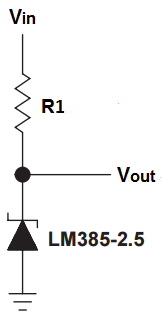
\includegraphics[scale=1.0]{figures/cProblemloesning/ReferenceEksempel}
	\caption{Figuren illustrerer et eksempel på opsætning af et kredsløb for en spændingsreference med LM$385$. Figuren er en revideret udgave fra kilden. \cite{Instruments2005}}
	\label{fig:Spaendingsreference}
\end{figure}

For at udregne værdien af modstanden, R, i kredsløbet, anvendes følgende generelle formel:
\begin{equation}
R=\dfrac{V_{forsyning}-V_{Reference}}{I_{Z}}
\end{equation}
Hvor V_{forsyning} er forsyningsspændingen som sendes ind i kredsløbet, V_{Reference} er den referencespænding der skal sendes ud af systemet og I_{Z} er strøm forbruget fra de komponenter, der er i referencespændings kredsløbet. 
\noindet \textbf{Beregning af referenceværdien til offset}
Først udregnes R for referencespændingen til offsettet. V_{forsyning} er de $5.5$V, der forsynes med fra spændingsforsyningen. V_{Reference} $2.5$V. I kredsløbet for ofsettet indgår én operationsforstærker(TL$081$), der har en maksimal biasstrøm på $200$pA\cite{Corporation1995}. Referencedioden har et arbejdsområde mellem $20\muA$ til $20mA$ og for at sikre der er strøm nok til referencedioden er den sat til at bruge $100\muA$\cite{Instruments2005}. Dermed kan strømforbruget, I_Z, for offsettet udregnes som summen af de to biasstrømme og alle de kendte værdier indsættes i formlen:

\begin{equation}
R_{offset}=\frac{5.5V-2.5V}{0.0001000002A}=29999.94\Omega \approx 30K\Omega
\end{equation}  
Da offsettet på accelerometeret er på $1.6325$V jævnført \ref{Offset_Teori_Design} på side \pageref{Offset_Teori_Design} skal referenceværdi være ligeledes $1.6325$V. For at opnå denne referenceværdi, bruges der en spændingsdeler. Den genelle formel for spændingsdeler er: 

\begin{equation} \label{Spaendingsdeler}
V_{out}=V_{in}*\dfrac{R2}{R1+R2}
\end{equation}

R$1$ bliver valgt til at være $10$K\Omega og derved er følgende kendt: 
\begin{itemize}
\item V_{out}  = $1.6325$V
\item V_{in} = $5.5$V
\item R1 = $10$K\Omega
\end{itemize}
Ligningen kommer til at være således: 
\begin{equation}
1.6325V = 5.5* \dfrac{R2}{10000\Omega+R2} 
R2 = 18818.44380\Omega \approx 18820\Omega
\end{equation}

\noindet \textbf{Beregning af referenceværdien til komparator}
Den samme fremgangsmåde anvendes til udregning af R for referencespændingen til komparatoren. Her er den ønskede referenceværdi  $2.5$V, så der benyttes ikke en spændingsdeler. Der er i begyndelse at kredsløbet indsat en operations forstærker (TL$082$), som har to input og output og derved kan fungere som både buffer til komparator kredsløbet og inverterende forstærker. Da spændingsdeleren går direkte ind i en buffer, så er den maksimale biasstrøm på $50nA$. Biasstrømmen for referencedioden er igen sat til $100\muA$. Dermed kan værdierne igen indsættes i formlen og R kan beregnes.

\begin{equation}
R_komparator=\frac{5.5V-2.5V}{0.000100005A}=29998.50007\Omega \approx 30K\Omega 
\end{equation} 

\textbf{Test af referencespænding}

 
\input{rapportAfsnit/eProblemloesning/Design/Offset/Offsetjustering}
% !TeX spellcheck = da_DK
\subsection{Forstærker i opsamlingsblok}\label{Subsec:Forstaerker}
\subsubsection{Teori og design}
Til forstærkningen i opsamlingsblokken på \figref{kravblok} skal der benyttes en ikke-inverterende forstærker, da der ønskes, at inputtet og outputtet har samme polaritet. Ved en ikke-inverterende forstærker bliver inputtet tilkoblet direkte til den ikke-inverterende inputterminal, som har en impedans på $10^{12}\Omega$ indbygget i operationsforstærkeren\cite{Corporation1995}. Hvis der var en lav indgangsimpedans, hvilket der kan være i den inverterende terminal grundet designet, ville denne blok trække strøm fra inputsignalet, hvilket kan give  afvigelser i de efterfølgende blokke. \\
Kredsløbet består af en operationsforstærker kaldet TL$081$, som sidder i et closed-loop med modstandene R$1$ og R$2$, der udgør en spændingsdeler. Dette ses på \figref{fig:Forstaerker}.
\begin{figure}[H]
\centering
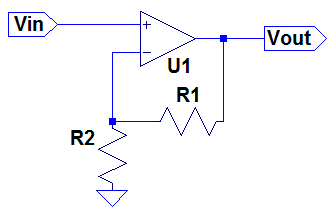
\includegraphics[scale=0.75]{figures/cProblemloesning/Forstaerker.PNG}
\caption{På figuren ses designet for en ikke-inverterende forstærker i en closed-loop konfiguration.}
\label{fig:Forstaerker}
\end{figure} 

\noindent Der er jævnfør afsnit \ref{OpsamlingsAfs} på side \pageref{OpsamlingsAfs} bestemt, at forstærkningen skal være en faktor $9.1$, hvilket svarer til $19.1808$dB. For at udregne R$1$ er R$2$ modstanden blevet valgt til $10$K$\Omega$. \cite{Nilsson2011} Ud fra dette er R$1$ blevet bestemt ved følgende udregning:
\begin{align}
9 = 1 + (\frac{R1}{10\text{K}\Omega})\\
R1 = 81\text{K}\Omega
\end{align}

\noindent R$1$ og R$2$ bliver brugt til at designe kredsløbet for en ikke-inverterende operationsforstærker. Dette kredsløb designes i LT-spice, som ses på \figref{fig:Forstaerker_faktor18}. 
\begin{figure}[H]
\centering
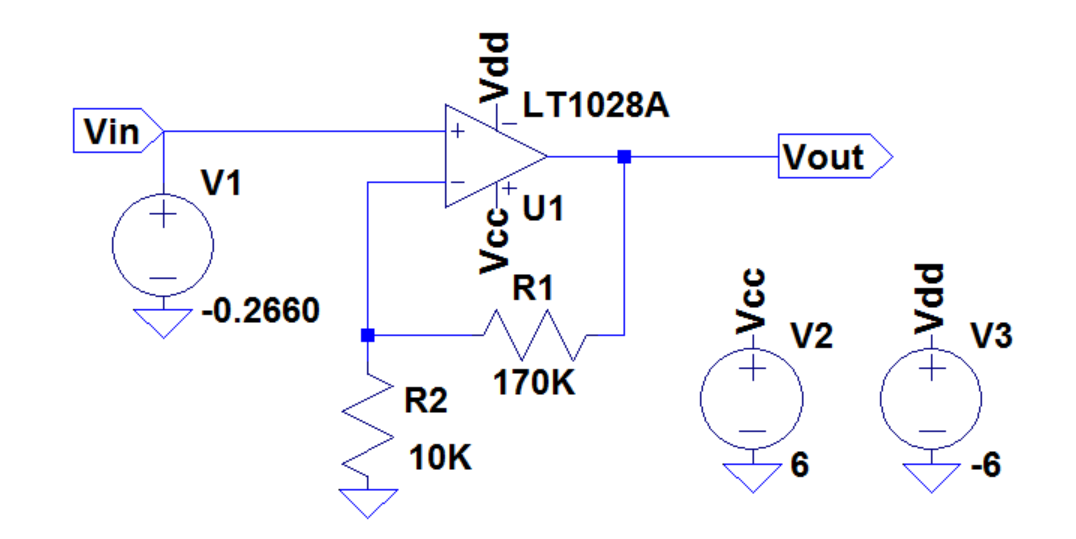
\includegraphics[scale=0.3]{figures/cProblemloesning/Forstaerker_faktor18.PNG}
\caption{På figuren ses designet at kredsløbet for en ikke-inverterende forstærker med to modstande. R$1$ og R$2$ har værdierne $81$K$\Omega$ og $10$K$\Omega$, hvilket giver en forstærkning med en faktor $9.1$.}
\label{fig:Forstaerker_faktor18}
\end{figure} 

\subsubsection{Simulering}\label{Subsec:Forstaerker_simu}
Der undersøges i to simuleringer, om forstærkeren virker ved det laveste input på $0.3233$V og højeste input på $0.3313$V, som er blevet udregnet igennem pilotforsøget. På \figref{fig:Forstaerker_faktor18_simulering} ses en simulering af dette.

\begin{figure}[H]
\centering
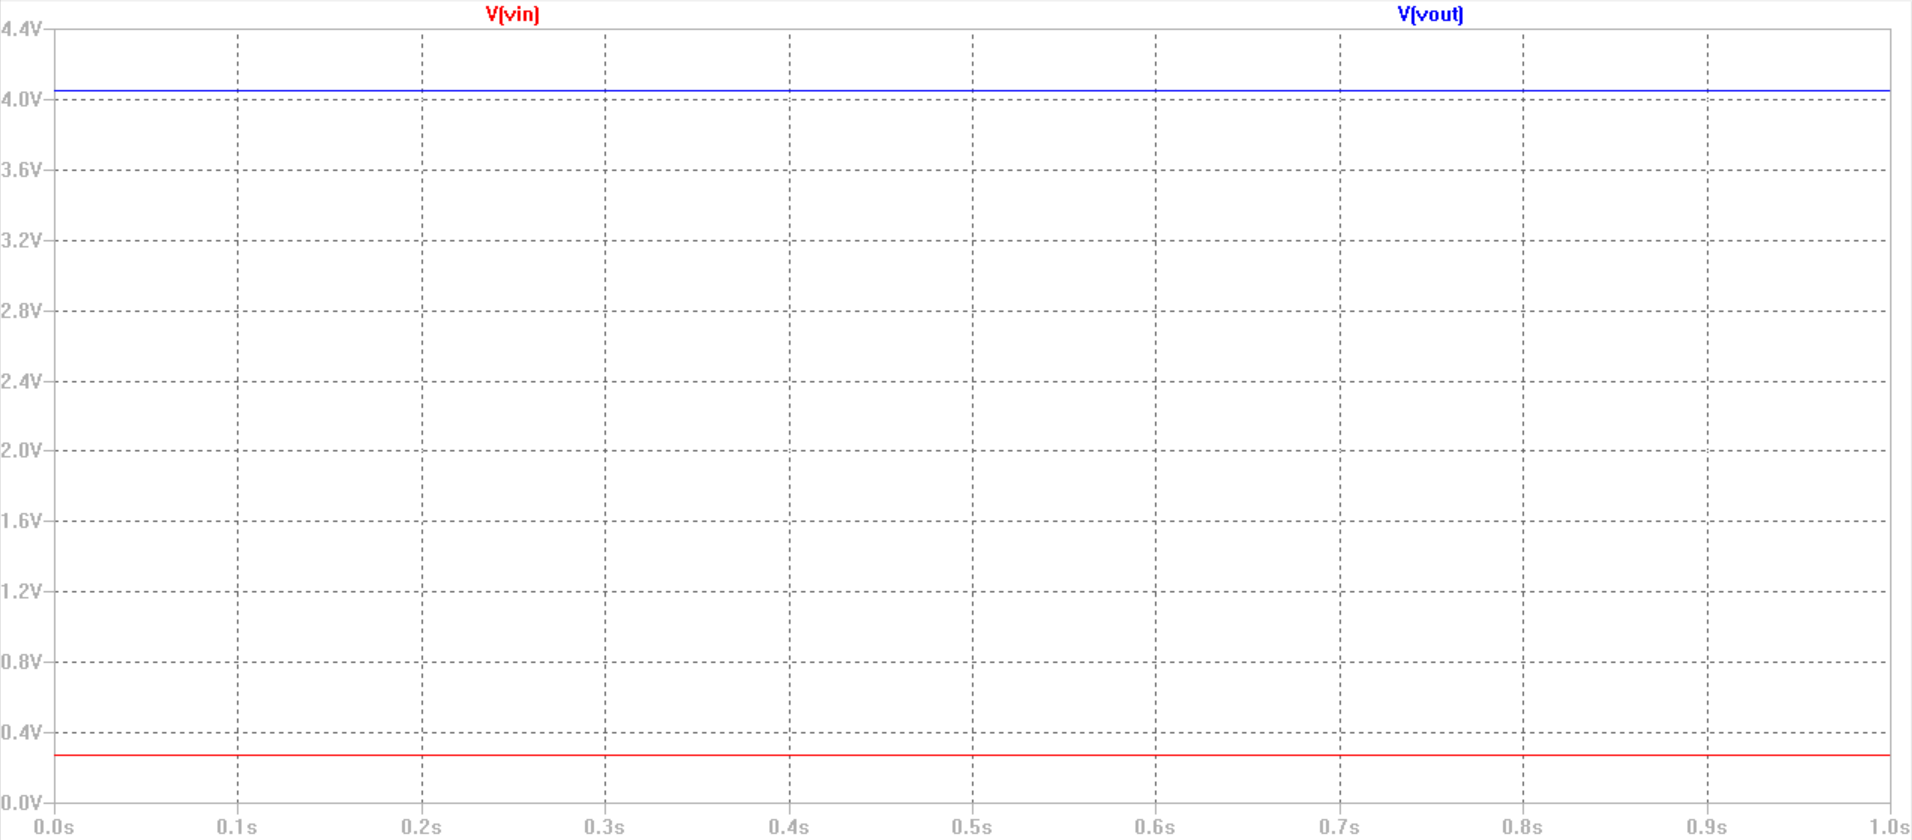
\includegraphics[scale=0.36]{figures/cProblemloesning/Forstaerker_faktor18_simulering.PNG}
\caption{På figuren ses en simulering af en ikke-inverterende forstærker, hvor der sker en forstærkning med en faktor $9.1$. Inputtet, $V_{in}$, er $0.3313$V, som bliver forstærket $9.1$ gange og derved giver ca. $3$V i outputtet, $V_{out}$.}
\label{fig:Forstaerker_faktor18_simulering}
\end{figure}

Der kan ses på \figref{fig:Forstaerker_faktor18_simulering}, at det forstærkede signal, kaldet $V_{out}$, er ca. $3$V, hvilket er ca. $9.1$ gange større end $V_{in}$, som i simuleringen er sat til $0.3313$V. Derved er der sket den ønskede forstærkning som forventet, da simuleringen er med ideelle komponenter. Derfor har de enkelte komponenter i denne simulering en lav tolerance, sammenlignet med komponenterne i et reelt kredsløb. \\
Resultaterne af de to simuleringer ses i \tableref{tab:forstarker18_sim}
\begin{table}[H]
	\centering
	\begin{tabular}{|l|l|l|l|l|}
		\hline
		\multicolumn{1}{|c|}{\textit{Inputsignalet}} & \multicolumn{1}{c|}{\textit{Forstærkning}} & \multicolumn{1}{c|}{Outputsignalet} &  \textit{Målte forstærkning}   & \textit{\begin{tabular}[c]{@{}l@{}}\% afvigelse\\ i forstærkning\end{tabular}} \\ \hline
		$0.3313$V      & $9.1$   & $3.0147$V    &  $9.10$  &   $0\%$  \\ \hline
%		$0$V           & 10       & $0$V          & $0.000206$V         & $0.0206$\%       \\ \hline
		-$0.3233$V     & $9.1$   & -$2.9417$V   &  $9.10$  &   $0\%$  \\ \hline
	\end{tabular}
	\caption{I tabellen ses resultaterne for simuleringerne med det laveste- og højeste input.}
	\label{tab:forstarker18_sim}
\end{table}
\noindent Der ses på afvigelserne, at der arbejdes med ideelle komponenter, da der er en lav afvigelse i outputtet ift. det forventede output. Derved fungerer kredsløbet teoretisk og kan implementeres.

\subsubsection{Implementering og test}
Ifølge det valgte design skal der benyttes to modstande på $10$K$\Omega$ og $81$K$\Omega$ til opbygningen af forstærkeren. Reelt findes der ikke en modstand på $81$K$\Omega$, hvorfor der istedet benyttes $82$K$\Omega$. Dette giver teoretisk en forskel på $1.235$\% i modstanden. Dette er det tætteste man kan komme på $81$K$\Omega$. Der kunne også benyttes en $150$K$\Omega$- og $180$K$\Omega$ modstand i parallel forbindelse, hvilket vil give $1.01$\% afvigelse. Disse komponenter vil også have afvigelser, hvorved den samlede procentvise afvigelse vil forøges. De to modstande blev målt inden testen, hvilket fremgår i \tableref{Tab:modstand_faktor18}.
\begin{table}[H]
	\centering
	\begin{tabular}{|l|l|l|}
		\hline
		\textit{Teoretisk} & \textit{Ved måling} & \textit{\% afvigelse} \\ \hline
		$10$K$\Omega$      & $10.0236$K$\Omega$    & $0.24$\%           \\ \hline
		$82$K$\Omega$      & $81.724$K$\Omega$     & $0.89$\%           \\ \hline
	\end{tabular}
	\caption{I tabellen ses det, at de to modstande afviger lidt fra deres teoretiske værdi, hvilket er forventet af reelle komponenter. Det er en acceptabel afvigelse ifølge tolerancerne i afsnit \ref{OpsamlingsAfs}, side \pageref{OpsamlingsAfs}. Modstandene kan derfor anvendes til implementeringen.}
	\label{Tab:modstand_faktor18}
\end{table}
\noindent Den $82$K$\Omega$ modstand har en $0.89\%$ afvigelse, men i dette tilfælde betragtes afvigelsen som positiv, da der ønskes en $81$K$\Omega$ modstand. Herefter blev kredsløbet implementeret. Til afbildning af signalet blev der benyttet et multimeter, som viste det forstærkede signal for de to spændingsniveauer. De aflæste resultater er angivet under "Output" i \tableref{Tab:faktor18_test}.\
\begin{table}[H]
	\centering
	\begin{tabular}{|l|l|l|l|l|}
		\hline
		\textit{Teoretisk input} & \textit{Målte input} & \textit{Output} & \% \textit{\begin{tabular}[c]{@{}l@{}}Faktiske\\ forstærkning\end{tabular}} & \textit{\begin{tabular}[c]{@{}l@{}}\% afvigelse\\ i forstærkning\end{tabular}} \\ \hline
		$0.3313$V   & $0.3310$V    & $3.0258$V       &    $9.14$   & $0.44\%$     \\ \hline
%		$0$V        & $0.3523$mV   & $3.5230$mV    & -$10$mV         & $38.49\%$      \\ \hline
		-$0.3233$V  & -$0.3231$V   & -$2.9612$V      &    $9.16$   & $0.66\%$     \\ \hline
	\end{tabular}
	\caption{I tabellen ses resultaterne fra testen med forstærkeren, der har en faktor $9.1$. Det maksimale og minimale input fra offsetjusteringen er blevet testet med.}
	\label{Tab:faktor18_test}
\end{table}
% Det "målte input" er her blevet målt med et multimeter. %For $0.3313$V er spændingen kommet direkte fra en strømforsyning, men for at undersøge forstærkningen af $-0.3233$V er det nødsaget at benytte offsettet, da spændingsforsyningen ikke kan levere en negativ spænding. Det var derfor forventet, at der kunne være en større afvigelse på målingerne med $-0.3233$V spænding, da denne spænding skulle igennem flere kredsløb. Inputtet i offsettet (som kan ses på \figref{fig:Offset_generisk}) var $1.3092$V og referencen var $1.6325$V. Derved skabes den negative spænding, som sendes videre til forstærkeren. Afvigelsen, som ville opstå grundet et ekstra kredsløb, ville være præsentabel for afvigelsen, som der også burde have været for de to andre signalers tests. Der ses i \tableref{Tab:faktor18_test}, at der ikke opstod større forstyrrelser, som gav ekstra afvigelse i det målte signal ift. det forventede signal. \\
Der ses ud fra testen, at forstærkeren overholder kravene fra afsnit \ref{OpsamlingsAfs}, side \pageref{OpsamlingsAfs}. Derudover ligger afvigelserne indenfor tolerancerne for forstærkningen, som er $\pm2\%$. Derfor anses disse afvigelser som acceptable.
% !TeX spellcheck = da_DK
\subsection{Filter}
\subsubsection{Teori og design}
%Efter signalet er blevet forstærket skal det filtreres, så alle de uønskede signaler kan dæmpes. Der benyttes kun et lavpasfilter, da det ønskede signal ifølge litteraturen kan ligge i frekvensområdet $0-10$Hz, som beskrevet i afsnit \ref{FilterAfs} på side \pageref{FilterAfs}. Jævnfør pilotforsøget i afsnit \ref{Sec:PilotforsoegKort}, side \pageref{Sec:PilotforsoegKort} blev der målt et signal i frekvensområdet $0-25$Hz og det frekvensområdet sættes derfor til $0-25$Hz, for at filtrere uønskede signaler fra. 
Filtre kan udarbejdes både i aktiv og passiv form. Hvis signalet ligger i frekvensområdet under $1$MHz anbefales det at benytte aktive filtre. Aktive filtre benytter operationforstærkere, kondensatorer og modstande, hvor passive filtre benytter kondensatorer, modstande og spoler. \cite{Carter2013} Der findes flere forskellige typer filtre, heriblandt Butterworth-, Tschebyschev- og Besselfilter. Butterworthfilteret giver maksimal fladhed i pasbåndet og stopbåndet. Tschebyschevfilteret giver den hurtigste overgang fra pasbåndet til stopbåndet. Besselfilteret giver en lineær faserespons, hvilket vil sige at fasen er lineær med frekvensen.\fxnote{Til os: Fasen angiver hvor godt et signals frekvensspektrum bliver gengivet}\fxnote{skal vi have et billede ind af de forskellige typer?} \cite{Carter2013} I dette projekt anvendes et Butterworthfilter, da der ønskes maksimal fladhed i pasbåndet og stopbåndet som nævnt i kravspecifikationerne for filtret. De forskellige typer filtre fremgår af nedenstående \figref{fig:type_filtre}. \fxnote{kilde?}

\begin{figure}[H]
	\centering
	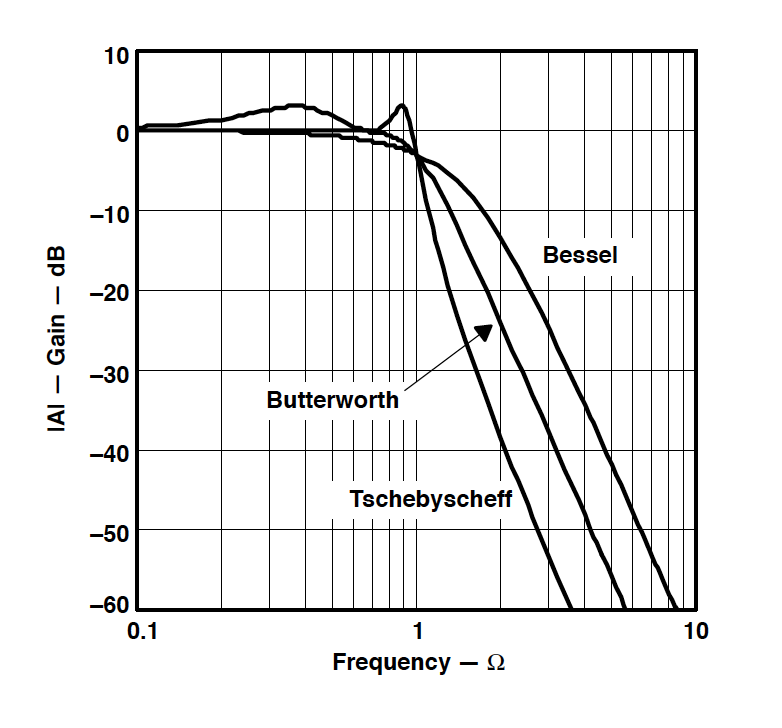
\includegraphics[scale=0.7]{figures/cProblemloesning/type_filtre.PNG}
	\caption{Figuren viser et bodeplot filter, hvor de fire karakteristika af et lavpasfilter er angivet}
	\label{fig:type_filtre}
\end{figure}

Der findes to forskellige måder hvorpå et filter kan designes: Sallen-Key topologien (SKT) og Multiple Feedback toppologien (MFT). SKT-metoden er den mest anvendte og tillader separate gain indstillinger samt inverterende og ikke-inverterende konfigurationer, hvorimod MFT-metoden benyttes i filter design med høj gain-nøjagtighed(Q-værdi). I dette projekt benyttes en ikke-inverterende konfiguration grundet den høje indgangsimpedans i den ikke-inverterende terminal, hvorfor SKT-metoden er valgt. Herved forhindres det, at filtret loader fra de forrige blokke. Loading defineres som effekten af, at et komponent trækker strømmen i et kredsløb f.eks. et måleapparat. Loading kan være både ønsket, hvis f.eks. brugen af strøm til aktivering af en LED-diode loader, og uønsket, hvis f.eks. et måleapparat trækker strøm ved afmåling af et signal, i et system. Loading vil trække i den samlede strøm fra kredsløbet, og trækker derfor meget strøm fra batterierne. Hvis der vælges et inverterende design for operationsforstærkeren i filterkonfiguration, vil blokken have en lav indgangsimpedans, hvorfor denne blok vil begynde at loade. Der kræves derfor mere strøm for at opretholde outputspændingsniveauet. \cite{Webster2009,Carter2013,Karni2014}

Jævnfør kravspecifikationer af lavasfilteret i afsnit \ref{FilterAfs}, side \pageref{FilterAfs} kræves det, at filteret har en minimumsdæmpning af stopbåndet $(min_{A})$ på $14$dB og der accepteres en maksimal dæmpning af pasbåndet $(max_{A})$ på $3$dB. Derudover skal lavpasfilteret have en pasbåndfrekvens $(\omega_p)$ på $25$ Hz, samt en stopbåndfrekvens $(\omega_s)$ på $45$ Hz. Af nedestående figur \figref{fig:lavpasfilter_generisk} fremgår en illustration af, hvad de forskellige parametre beskriver.

\begin{figure}[H]
	\centering
	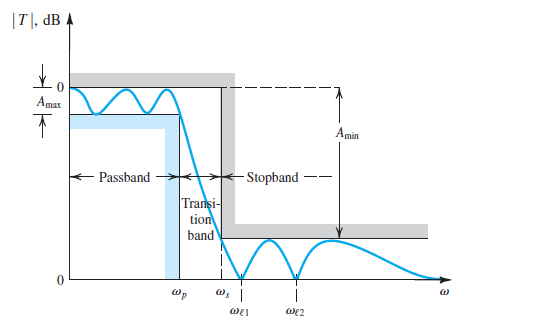
\includegraphics[scale=1]{figures/cProblemloesning/Lavpasfilter_generisk.PNG}
	\caption{Figuren viser et bodeplot filter, hvor de fire karakteristika $(min_{A})$, $(max_{A})$, $(\omega_p)$ og $(\omega_s)$ af et lavpasfilter er angivet. \cite{Carter2013}}
	\label{fig:Lavpasfilter_generisk}
\end{figure}
\noindent Med udgangspunkt i de enkelte parametre af lavpasfilteret kan den pågældende orden af filteret bestemmes vha. \eqref{lavpasfilter} for overføringsfunktionen:
\begin{equation} \label{eq:lavpasfilter}
A(\omega_s) = 10 \text{log} \cdot \left[1 + \epsilon^2 \cdot (\frac{\omega _s}{\omega _p})^{2N}\right] 
\end{equation}

\noindent I \eqref{eq:lavpasfilter} betegner $A(\omega _s)$ den minimale dæmpning der kræves af stopbåndet. $(\omega_p)$ og $(\omega_s)$ er pasbåndfrekvensen og stopbåndfrekvensen, som begge er angivet i Hz. Disse variable kan ses på \figref{fig:Lavpasfilter_generisk}. N angiver filtrets orden, og $\epsilon$ er udtrykt ved nedenstående \eqref{epsilon}:
\begin{equation}\label{eq:epsilon}
\epsilon = \sqrt{10^{A_{max} / 10} -1}
\end{equation}

Nu kan lavpasfilterets orden bestemmes, jævnfør værdierne fra kravspecifikationerne fra afsnit \ref{FilterAfs}, side \pageref{FilterAfs} ved at indsætte disse værdier i \eqref{eq:lavpasfilter}. Udregningerne vil se ud som følgende:
\begin{equation}
\epsilon = \sqrt{10^{3dB /10} -1} = 0.998 \\ \label{eq:orden}
14\text{dB} = 10 \cdot \text{log} \left[1 + \epsilon ^2 \cdot (\frac{45\text{Hz}}{25\text{Hz}})^{2N}\right] \\
N = 2.711 \approx 3
\end{equation}
\noindent Det fremgår af \eqref{eq: orden}, at lavpasfilterets orden bliver $3$. Filterets orden kun kan angives i hele tal og derfor afrundes resultatet. Hvis kravene til filteret skal overholdes, skal der altid rundes opad ved udregning af orden.

Der skal altså benyttes et 3. ordens lavpasfilter. I dette tilfælde anvendes filtertypen, SKT. Et 3. ordens lavpasfilter konstrueres ved at sammenætte et 1. ordens filter med et 2. ordens filter. Af figur \figref{fig:SallenKey1} og \figref{fig:SallenKey2} fremgår hhv. et 1. og 2. ordens lavpasfilter designet efter SKT. \cite{Carter2013}
	
\begin{figure}[H]
	\centering
	\begin{minipage}[b]{0.45\textwidth}
		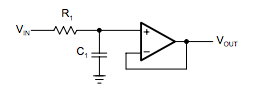
\includegraphics[width=\textwidth]{figures/cProblemloesning/Lavpasfilter1_teoretisk.PNG}
		\caption{På figuren ses en illustration af et 1. ordens unity-gain Sallen-Key lavpasfilter, hvor værdien C er kondensatoren, R er modstandene. filterKonfigurationen har en indgangsspænding, Vin og udgangsspænding, Vout. \citep{Carter2013}}
		\label{fig:SallenKey1}
	\end{minipage}
	\hfill
	\begin{minipage}[b]{0.45\textwidth}
		\includegraphics[width=\textwidth]{figures/cProblemloesning/Sallenlavpas.PNG}
		\caption{På figuren ses en illustration af et 2. ordens unity-gain Sallen-Key lavpasfilter, hvor værdien C er kondensatoren, R er modstandene. filterKonfigurationen har en indgangsspændings, Vin og en udgangsspænding, Vout. \citep{Carter2013}}
		\label{fig:SallenKey2}
	\end{minipage}
\end{figure}

I designet af et 3. ordens filter designes både et 1. og et 2. ordens filter i forlængelse af hinanden, som ses på \figref{fig:filter_Orden}.
\begin{figure}[H]
	\centering
	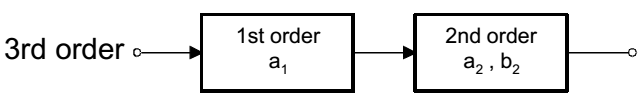
\includegraphics[scale=1]{figures/cProblemloesning/Filter_Orden.PNG}
	\caption{På figuren ses, hvordan et 3. ordens filter designes ved et 1.- og 2. ordens filter i forlængelse af hinanden. Værdierne $a_{1}$, $a_{2}$ og $b_{2}$ er fastsatte værdier, som kan aflæses i en tabel for Butterworth koefficienterne. \cite{Carter2013}}
	\label{fig:filter_Orden}
\end{figure}
\noindent Filtret designes efter SKT-metoden bestående af tre modstande, tre kondensatorer og to operationsforstærkere. Værdierne for modstandene kan udregnes ved \eqref{eq:Lavpas1Modstande} for et 1. orden lavpasfilter, der skal benytte en modstand, kondensator og operationsforstærker. I \eqref{eq:LavpasModstande} udregnes modstandene for et  2. orden lavpasfilter, der skal benytte to modstande, to kondensatorer og en operationsforstærker. \cite{Carter2013}
\begin{equation} \label{eq:Lavpas1Modstande}
R_{1} = \frac{a_1}{2 \cdot \pi \cdot f_c \cdot C_1} \\
\end{equation}
\begin{equation}
 \label{eq:LavpasModstande}
R_{2,3} = \frac{a_2 \cdot C_3 \pm \sqrt{{a_2}^2 \cdot C_3^2 - 4 \cdot b_2 \cdot C_2 \cdot C_3}}{4 \pi \cdot f_c \cdot C_2 \cdot C_3}
\end{equation}
\noindent Værdien for $C_{1}$ i \eqref{eq:Lavpas1Modstande} og \eqref{eq:LavpasModstande} er nødvendigvis ikke det samme, da disse to ligninger er uafhængige af hinanden. Der aflæses i en tabel for Butterworth koefficienterne, at $a_{1}$, $a_{2}$ og $b_{2}$ skal være 1.0000. For at finde reelle værdier under kvadratroden i \eqref{eq:LavpasModstande} skal følgende være opfyldt:
\begin{equation} \label{eq:kondensator}
C_3 \geq C_2 \frac{4 \cdot b_2}{a_2^2}
\end{equation}
I \eqref{eq:LavpasModstande} står C for kondensatorer, R står for modstande og $a_1$ og $b_1$ er konstanter, mens $f_c$ er den valgte knækfrekvens i Hz, jævnfør kravspecifikationerne afsnit \ref{FilterAfs} på side \pageref{FilterAfs}. 

\noindent For at udregne modstandene fastsættes $C_1$ til 100nF for hhv. både 1. og 2. ordens lavpasfiltrene. Når $C_1$ er bestemt, kan $C_2$ for 2. ordens lavpasfilteret beregnes ved at benytte følgende \eqref{eq:kondensator}. Som grundregel skal $C_3$ være over dobbelt så stor som $C_2$:
\begin{equation}  
C_3 \geq 100\text{nF} \frac{4\cdot 1}{1.000^2} = C_3 \geq 400\text{nF}
\end{equation}

\noindent Ud fra ovenstående ligning vælges $C_3$ til at være 470nF for at opfylde \eqref{eq:kondensator}. Når værdierne for C er bestemt kan modstandene for filteret bestemmes. For et 1. orden lavpasfilter benyttes \eqref{eq:Lavpas1Modstande} til at beregne $R_1$ og for et 2. ordens lavpasfilter anvendes \eqref{LavpasModstande} for at beregne $R_1$ og $R_2$. 
\begin{equation} \label{eq:1ordenmodstand}
R_{1} = \frac{1}{2 \cdot \pi \cdot 25 \cdot 100nF} R_{1} = 63661.98 \Omega
\end{equation}
\begin{equation} \label{eq:2ordenmodstand}
R_{2,3} = \frac{1.0000 \cdot 470\text{nF} \pm \sqrt{1.0000^2 \cdot 470\text{nF}^2 - 4 \cdot 1.0000 \cdot 100\text{nF} \cdot 470\text{nF}}}{4 \pi \cdot 25\text{Hz} \cdot 100\text{nF} \cdot 470\text{nF}} = \begin{cases} R_{2} = 19546.69414 \Omega \\ R_{3} =  44115.28306 \Omega \end{cases}
\end{equation}
\noindent Filterets værdier for kondensatoerne og modstandene er nu udregnet for hhv. 1. og 2. ordens filter. Filterkonfigurationen kan nu simuleres i LTspice for at bestemme, hvor godt et 3. ordens filter, der er blevet designet.

\begin{figure}[H]
	\centering
	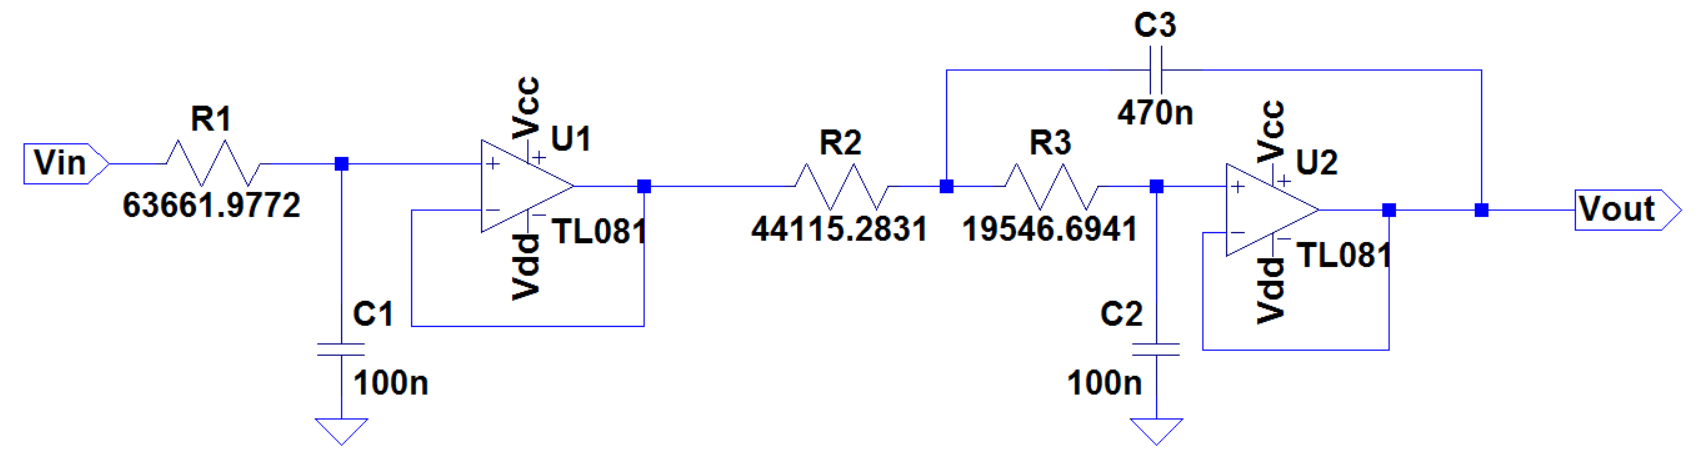
\includegraphics[scale=0.3]{figures/cProblemloesning/Lavpasfilter1_LTspice.PNG}
	\caption{På figuren ses det teoretiske kredsløb for lavpasfilteret med udregnede værdier for de enkelte modstande og kondenstatorer. Filteret er designet i LTspice.}
	\label{fig:lavpasfilter1_LTspice}
\end{figure}

\subsubsection{Simulering}
For at udføre en simulering af 3. ordens lavpasfilteret, foretages en AC-analyse, der beskriver forholdet mellem frekvensindholdet og filterets dæmpning. Kredsløbet simuleres med et inputsignal, der har en amplitude på $1$V. Der foretages en simulering ud fra kravspecifikationerne i afsnit \ref{FilterAfs} på side \pageref{FilterAfs}. LTspice anvendes til simulering af lavpasfilteret, hvor der anvendes operationsforstærkeren, TL081, hvilket er den operationsforstærker, der også vil blive benyttet i test af filteret. I simuleringen vil der blive undersøgt, hvorledes kravene stemmer overens med kravspicifikationerne, ved at betragte et bodeplot over det simulerede 3. ordens filter.

\begin{figure}[H]
	\centering
	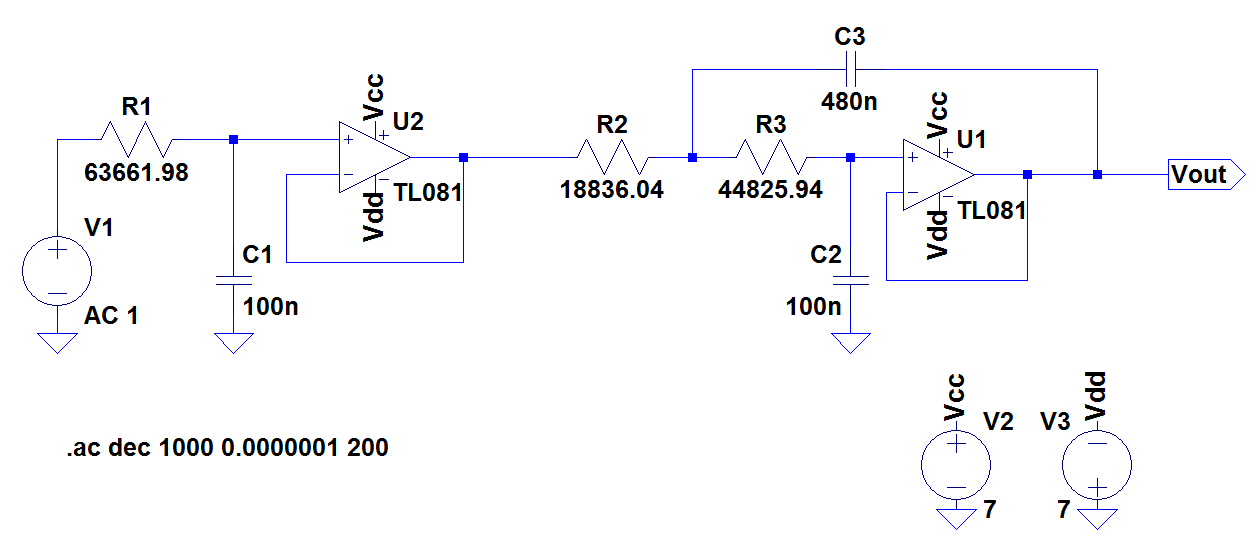
\includegraphics[scale=0.45]{figures/cProblemloesning/Lavpasfilter_LTspice.PNG}
	\caption{Af figuren fremgår en illustration af kredsløbet for et 3. ordens lavpasfilter. Filteret simuleres i LTspice vha. en AC-analyse med et inputsignal, der har en amplitude på $1$V.}
	\label{fig:lavpasfilter_LTspice}
\end{figure}

\begin{figure}[H]
	\centering
	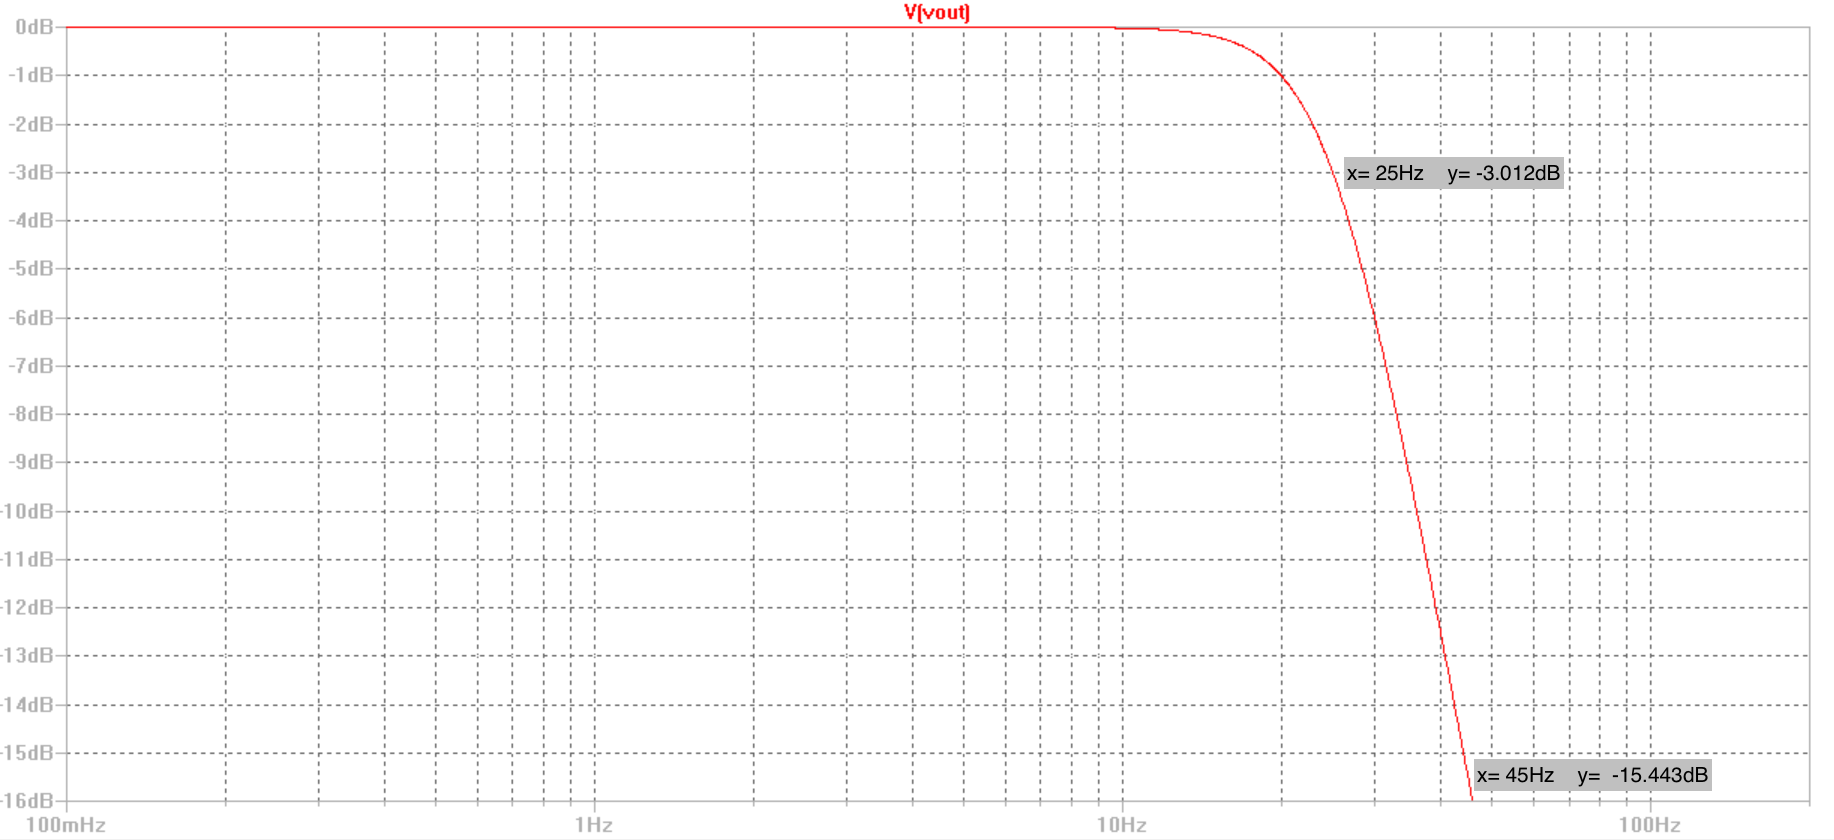
\includegraphics[scale=0.4]{figures/cProblemloesning/Lavpasfiltergraf_LTspice1.PNG}
	\caption{Af figuren fremgår en illustration på et bodeplot, der viser 3. ordens filterets frekvensindhold målt i Hz over dæmpningen målt i dB. Lavpasfilteret er simuleret i LTspice.}
	\label{fig:lavpasfilter_LTspice}
\end{figure}
\noindent Af bodeplottet fremgår det, at det simulerede filter har en maksimal amplitude i db på $-3.012$ ved en knækfrekvens på $25$Hz, hvilket ikke overholder kravspecifikationerne i afsnit \ref{FilterAfs}, side \pageref{FilterAfs}. Grundet den lave afvigelse accepteres afvigelsen i midlertidigt og der udføres derfor endnu en simulering af filteret med de reelle modstande, der kan benyttes under implementeringen. Der aflæses, at der ved en stopbåndsfrekvens på $45$Hz er amplituden i db på $-15.443$. Dette overholder projektets opstillede krav for filterkonfigurationen ved en minimum dæmpning på $14$ dB i stopbåndsfrekvensen. Filterkonfigurationen med reelle modstande fremgår af nedenstående \figref{Sim_reel_modstande}. Reelt findes de udregnede modstande ikke, hvorfor der benyttes de modstande der kommer tættest på den teoretiske værdi. 

%\begin{figure}[H]
%	\centering
%	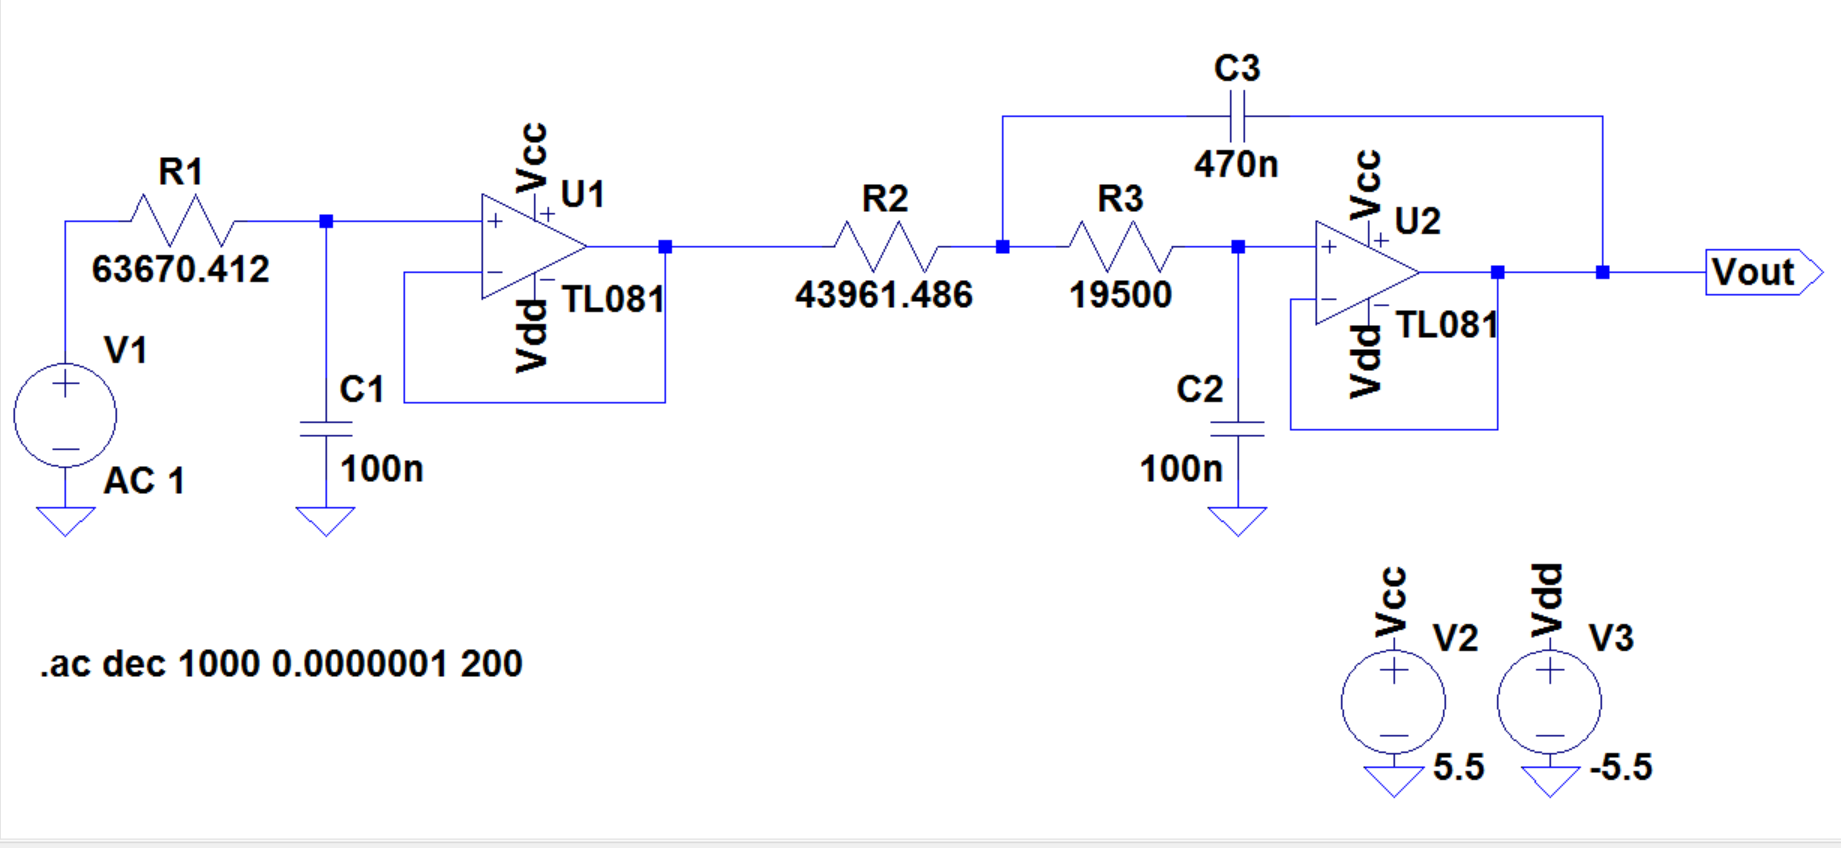
\includegraphics[scale=0.4]{figures/cProblemloesning/Sim_reel_modstande.PNG}
%	\caption{Af figuren fremgår et 3. ordens filter med reelle modstande, hvor R$1$ er parallel med $68$K $\Omega$ og $1$M $\Omega$, R$2$ er er parallel med $47$K $\Omega$ og $680$K $\Omega$ og R$3$ er parallel med to $32$K $\Omega$ modstande.}
%	\label{fig:Sim_reel_modstande}
%\end{figure}
%
%\begin{figure}[H]
%	\centering
%	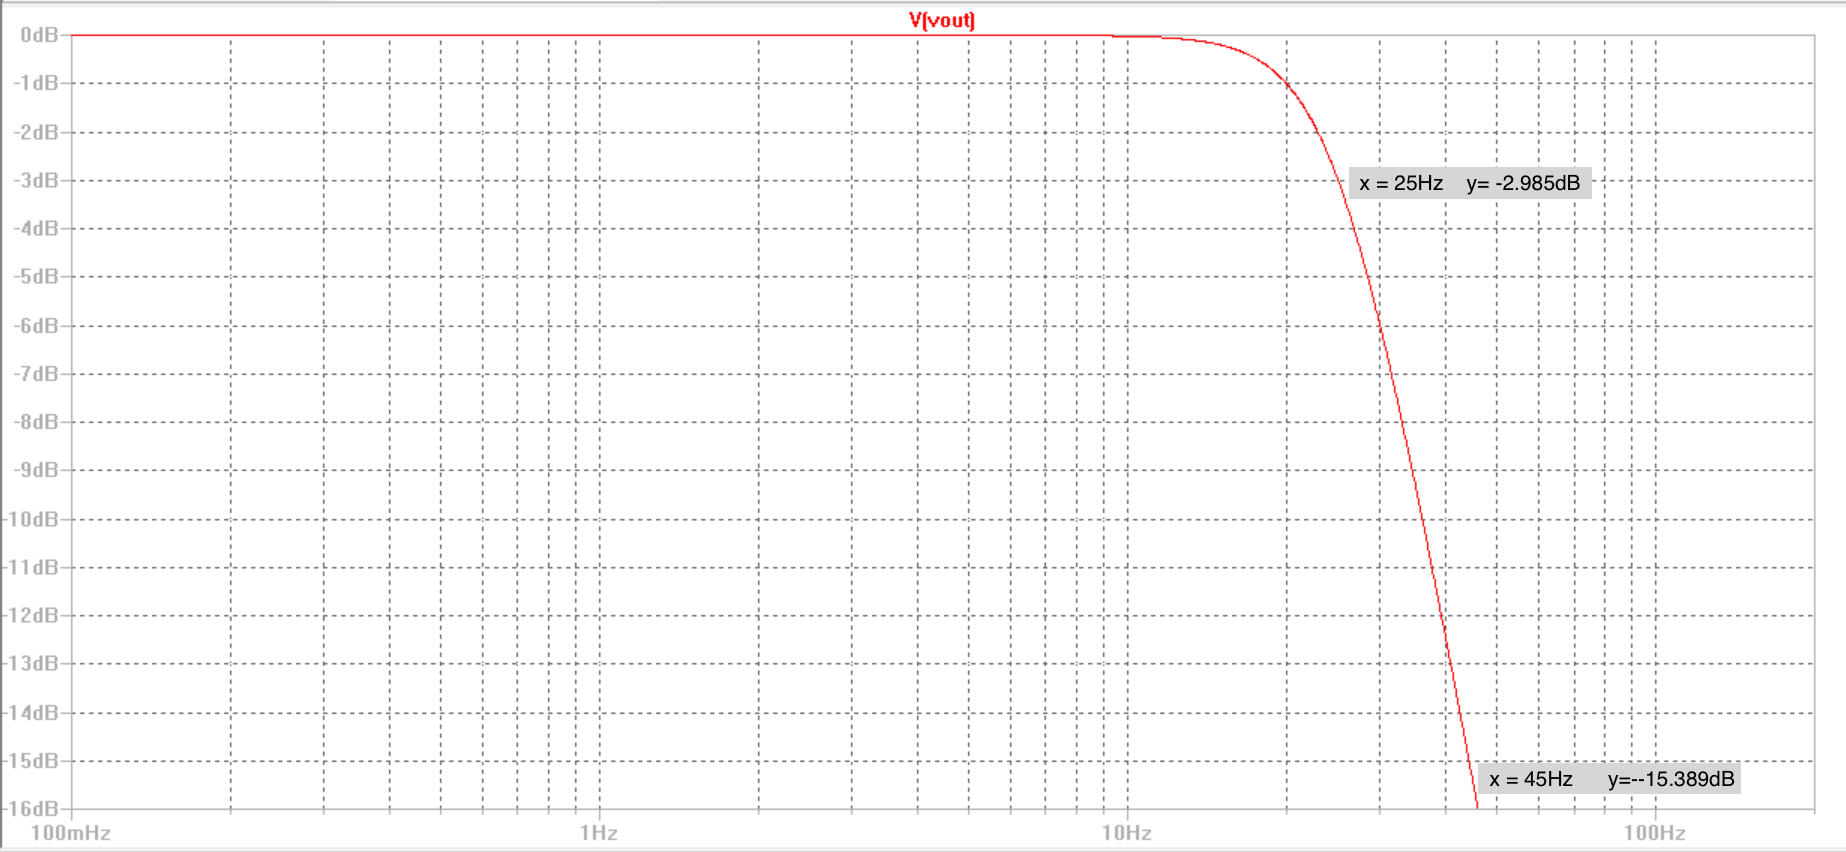
\includegraphics[scale=0.4]{figures/cProblemloesning/Sim_reel_graf.PNG}
%	\caption{Af figuren fremgår en illustration af et bodeplot, der viser 3. ordens filterets frekvensindhold målt i Hz over dæmpningen målt i dB med reelle modstande. Lavpasfilteret er simuleret i LTspice.}
%	\label{fig:Sim_reel_graf}
%\end{figure}

\noindent af bodeplottet det, at det simulerede filter med reelle værdier har en maksimal amplitude i dB $-2.985$ ved en knækfrekvens på $25$Hz, hvilket overholder kravspecifikationerne i afsnit \ref{FilterAfs}, side \pageref{FilterAfs}. Der aflæses, at ved stopbåndsfrekvensen på $45$Hz er amplituden i db $-15.389$, hvilket fortsat er acceptabelt ift. kravspecifikationerne for filterkonfigurationen. 

\subsubsection{Implementering og test} 
Der ses på \figref{fig:lavpasfilter_LTspice} at der benyttes 3 modstande og 2 kondensatorer til at designe kredsløbet. Af \tableref{Tab:Maalingfilter} fremgår, hvorledes modstandene sammensættes for at få de ønskede værdier, der fremgår i \figref{Sim_reel_modstande}, samt modstandenes afvigelse fra de ideelle modstande. For at finde afvigelsen er der foretaget målinger på tre ens reelle modstande og kondensatorer og på denne måde vurderes det, hvilke komponenter, der afviger mindst fra de teoretiske værdier. Dette er ydermere illustreret i \tableref{Tab:Maalingfilter}.
\begin{table}[H]
	\centering
	\begin{tabular}{|l|l|l|l|}
		\hline
		\textit{}                                     & \textit{Teoretisk} & \textit{Måling}    & \textit{Afvigelse} \\ \hline
		\multirow{2}{*}{\textit{$R_{1}$(Parallel) :}} & $1$M$\Omega$       & $1.0046$M$\Omega$  & $0.46\%$           \\ \cline{2-4} 
		                                              & $68$K$\Omega$      & $68.0350$K$\Omega$ & $0.05\%$           \\ \hline
		\multirow{2}{*}{\textit{$R_{2}$(Parallel) :}} & $680$K$\Omega$     & $1.0037$K$\Omega$  & $0.37\%$           \\ \cline{2-4} 
	                                               	  & $47$K$\Omega$      & $47.0540$K$\Omega$ & $0.11\%$           \\ \hline
		\multirow{2}{*}{\textit{$R_{3}$(Parallel) :}} & $32$K$\Omega$      & $17.9600\Omega$    & $0.22\%$           \\ \cline{2-4} 
		                                              & $32$K $\Omega$     & $816\Omega$        & $0.49\%$           \\ \hline
		\textit{$C_{1}$ :}                            & $100$n             & $98$n              & $2.00\%$           \\ \hline
		\textit{$C_{2}$ :}                            & $470$n             & $464$n             & $1.29\%$           \\ \cline{2-4} 
		\textit{$C_{3}$ :}                            & $100$n             & $98$n              & $2.00\%$           \\ \hline
	\end{tabular}
	\caption{I tabellen ses der, at de anvendte modstande og kondensatorer afviger fra den teoretiske værdi, hvilket er forventet af reelle komponenter. Det er en acceptabel afvigelse, så modstandene kan derfor anvendes til implementering}
	\label{Tab:Maalingfilter}
\end{table}
Herefter implementeres kredsløbet. I testen anvendes en spændingsforsyning på $5.5$V og en funktionsgenerator som inputsignal, samt et multimeter til aflæsning af dæmpningen. Funktionsgeneratoren sættes til de ønskede frekvenser i intervaller af $1$Hz fra $10$Hz til $50$Hz. Outputtet i dB måles for hver frekvens. Ud fra disse målinger plottes en graf af dæmpningen i MatLab, hvilket er illustreret på \figref{fig:Lavpas_Matlab}.  

\begin{figure}[H]
	\centering
	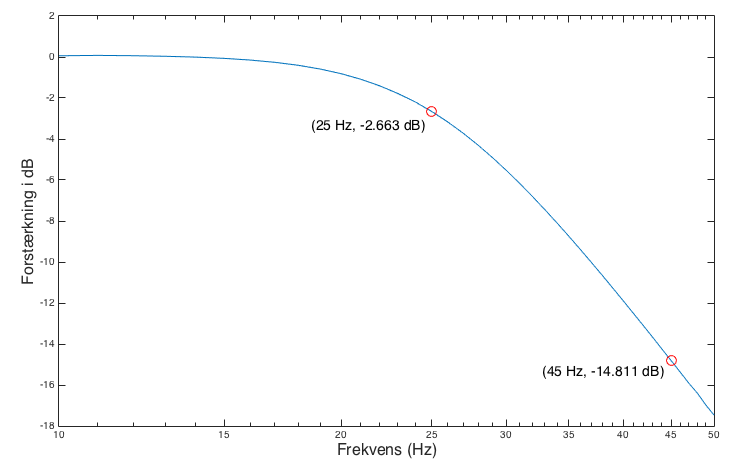
\includegraphics[scale=0.4]{figures/cProblemloesning/Lavpas_Matlab.PNG}
	\caption{Figuren viser dæmpningen som en graf over de målte frekvenser i Hz som funktion af outputtet i dB. På grafen er der angivet knækfrekvens og stopbåndfrekvens}
	\label{fig:Lavpas_Matlab}
\end{figure}

%Sammenlignes værdierne fra \ref{Lavpas_Matlab} for det testede kredsløb med værdierne fra \ref{fig:lavpasfilter_LTspice} for det simulerede kredsløb ses der en ændring i frekvens og dæmpning, hvilket også er forventet grundet andre kodensatorer og modstande. 

%\begin{table}[H]
%	\centering
%	\begin{tabular}{|l|l|l|l|}
%		\hline
 %  & \textit{Simulering} 	& \textit{Test}  &\textit{Afvigelse} \\ \hline
%Knækfrekvens	 & $25Hz$ 			& $25.0308Hz$			& $4\%$  \\ %\hline
%Stopbåndsfrekvens & $45Hz$		& $45.0816Hz$			& $0.18\%$ \\ \hline
%Dæmpning på stopbånd & $15.489dB$  & $14.881dB$     & $9.61\%$  \\ \hline
%Dæmpning på pasbånd & $3.0273dB$	  & $2.663dB$  & $13.68\%$  \\ \hline
%	\end{tabular}
%	\caption{I tabellen ses afvigelserne for hhv. knækfrekvens, stopbåndsfrekvens og dæmpning af stopbånd og pasbånd ift. simlering og test}
%	\label{Tab:Afvigelse_simulering}
%\end{table}

Ud fra de testede værdier i \tableref{Tab:Tolerance} og kravspecifikationer i afsnit \ref{filterAfs} på side \pageref{filterAfs} er der er ingen afvigelse på knækfrekvensen og stopbåndsfrekvensen. Der er en variation ift. dæmpningen for både stop- og pasbånd på hhv. $6.36\%$ og $8.37$\% i forhold til kravet.

\begin{table}[H]
	\centering
	\begin{tabular}{|l|l|l|l|}
		\hline
   & \textit{Krav} 	& \textit{Test}  &\textit{Afvigelse} \\ \hline
Knækfrekvens	 & $25Hz$ 			& $25Hz$			& $0\%$  \\ \hline
Stopbåndsfrekvens & $45Hz$		& $45Hz$			& $0\%$ \\ \hline
Dæmpning på stopbånd & $14dB$    & $14.8910dB$    & $6.36\%$  \\ \hline
Dæmpning på pasbånd & $3dB$		& $2.7490dB$	    & $8.37\%$ \\ \hline
	\end{tabular}
	\caption{I tabellen ses afvigelserne for hhv. knækfrekvens, stopbåndsfrekvens og dæmpning af stopbånd og pasbånd ift. krav og test}
	\label{Tab:Tolerance}
\end{table}
\noindent I forhold til tolerancekravene i afsnit \ref{FilterAfs} på side \pageref{FilterAfs} skulle dæmpningen på stopbåndet være minimum $14 dB$ og måtte maksimalt have en afvigelse herfra på $+10\%$. Denne tolerance overholdes ved testen, da de acceptable dæmpningsværdier vil ligge i intervallet $14$-$15.4$db. For pasbåndet skulle dæmpningen maksimalt være $3$dB med en maksimal afvigelse på $-15\%$. Dette vil sige at testen passer inden for tolerancekravene, da der accepteres værdier i intervallet $2.55$-$3$dB. På baggrund af dette accepteres alle målte afvigelser ved testen af filteret.
% !TeX spellcheck = da_DK
\subsection{Forstærker i tilpasningsblok}\label{Forstaerker_faktor3_afs}
\subsubsection{Teori og design}
I afsnit \ref{Subsec:Forstaerker}, side \pageref{Subsec:Forstaerker} er teorien samt designet af en forstærker forklaret. Da blokken tilpasning skal tilpasse det filtrerede signal til komparatoren, afgrænses måleintervallet til $\pm25^{\circ}$. Et range på $\pm90^{\circ}$ er unødvendigt ift. at vurdere hvorvidt patienten er faldet. Derfor ønskes det, at $V_{out}$ fra denne blok er $\pm3$V, når accelerometret måler $\pm25^{\circ}$. Der skal dermed ske en forstærkning med en faktor $3.6$, hvilket svarer til $11.1261$dB, som beskrevet i afsnit \ref{Tilpasningsblok} på side \pageref{Tilpasningsblok}. \\
For at udregne modstandene er R$2$ blevet valgt til $10$K$\Omega$. Ud fra dette er R$1$ blevet bestemt ved følgende udregning:
\begin{equation}
3.6 = 1 + (\frac{R1}{10\text{K}\Omega}) \\
R1 = 26\text{K}\Omega
\end{equation}

\noindent Forstærkerens opbygning kan ses på \figref{fig:Forstaerker_faktor3}.
\begin{figure}[H]
	\centering
	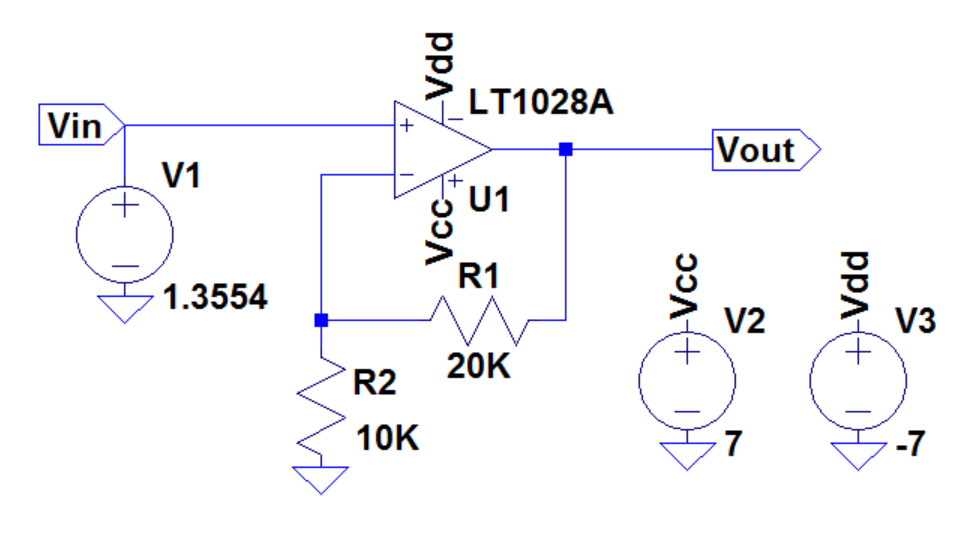
\includegraphics[scale=0.35]{figures/cProblemloesning/Forstaerker_faktor3.PNG}
	\caption{På figuren ses opbygningen af den ikke-inverterende forstærker, der forstærker med en faktor $3.6$.}
	\label{fig:Forstaerker_faktor3}
\end{figure}

\subsubsection{Simulering}
Forstærkeren testes i fire simuleringer for at undersøge, om den opfylder de opstillede krav. Det forstærkede signal($V_{out}$), skal være $3.6$ gange større end blokkens inputsignal($V_{in}$). Resultaterne af fire simuleringer ses i \tableref{tab:forstarker3_simT}. Der er benyttet de teoretiske værdier, som er udregnet fra start.
\begin{table}[H]
	\centering
	\begin{tabular}{|l|l|l|l|l|l|}
		\hline
		\multicolumn{1}{|c|}{\textit{Inputsignalet}} & \textit{\begin{tabular}[c]{@{}l@{}}For-\\stærkning\end{tabular}} & \textit{\begin{tabular}[c]{@{}l@{}}Forventet\\outputsignal\end{tabular}} & \multicolumn{1}{c|}{\textit{Outputsignalet}} & \textit{\begin{tabular}[c]{@{}l@{}}For-\\stærkning\end{tabular}}  & \multicolumn{1}{c|}{\textit{Afvigelse}} \\ \hline
		$3.0148$V     & $3.6$   & \begin{tabular}[c]{@{}l@{}}Forventer mætning\\ $10.8533$V\end{tabular} & $3.9765$V  & $\times$ & $\times$     \\ \hline
		$0.8418$V    & $3.6$   & $3.0305$V                                                              & $3.0304$V  & $3.6$ & $0\%$     \\ \hline
%		$0$V          & 3   & $0$V                                                                   & $33.6527\mu $V        & $\approx 0\%$     \\ \hline
	   -$0.8190$V     & $3.6$   & -$2.9484$V                                                             & -$2.9482$V  & $3.6$ & $0\%$     \\ \hline
	   -$2.9420$V     & $3.6$   & \begin{tabular}[c]{@{}l@{}}Forventer mætning\\ -$10.5912$V\end{tabular}& -$3.97703$V  & $\times$ & $\times$     \\ \hline
	\end{tabular}
		\caption{I tabellen ses resultaterne af de fire simuleringer.}
		\label{tab:forstarker3_simT}
\end{table}
\noindent Der ses i \tableref{tab:forstarker3_simT}, at der er en lav afvigelse er i forstærkningen, men dette lægger inde for referencerne. Kredsløbet fungerer rent teoretisk med ideelle komponenter, som bliver brugt i LTspice. På \figref{fig:faktor3_simulering} ses simuleringen af et inputsignal på $0.8325$V, som ideelt vil komme fra filtreringsblokken, hvis accelerometret hælder i $25^{\circ}$.

\begin{figure}[H]
	\centering
	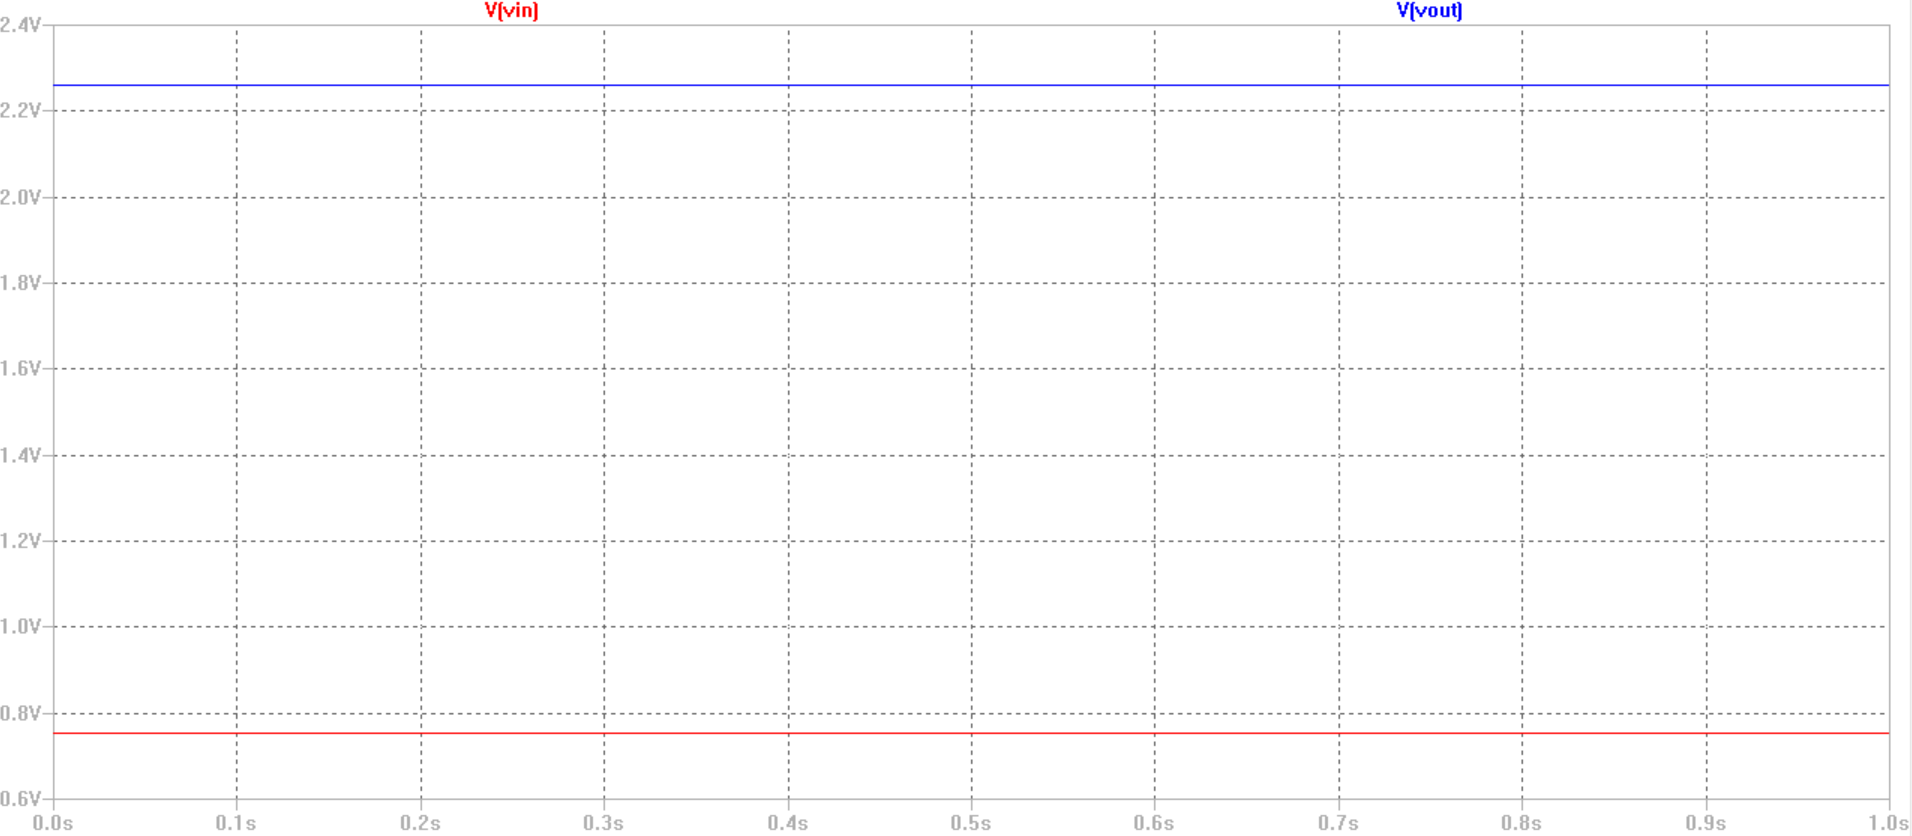
\includegraphics[scale=0.3]{figures/cProblemloesning/Forstaerker_faktor3_simulering.PNG}
	\caption{På figuren ses simuleringen for et inputsignal på $0.8418$V, som giver $3.0304$V i output. Der er således sket en forstærkning med en faktor $3.6$.}
	\label{fig:faktor3_simulering}
\end{figure}
\noindent Der ses på afvigelserne, at der arbejdes med ideelle komponenter. Det er herved bevist, at kredsløbet fungerer teoretisk og kan derfor implementeres.

\subsubsection{Implementering og test}
På \figref{fig:Forstaerker_faktor3} kan der ses, at der skal benyttes to modstande på $10$K$\Omega$ og $26$K$\Omega$ til opbygningen af forstærkeren. Reelt findes der dog ikke en $26$K$\Omega$, hvorfor der istedet benyttes $27$K$\Omega$- og $680$K$\Omega$ modstande i parallel forbindelse, hvilket teoretisk vil give en $0.12$\% afvigelse fra en ideelt $26$K$\Omega$ modstander. Disse tre modstande blev målt inden implementering, hvilket fremgår i \tableref{Tab:modstand_faktor18}.
\begin{table}[H]
	\centering
	\begin{tabular}{|l|l|l|}
		\hline
		\textit{Teoretisk}  & \textit{Ved måling} & \textit{\% afvigelse} \\ \hline
		$10$K$\Omega$       & $9.98$K$\Omega$     & $0.20$\%               \\ \hline
		$26$K$\Omega$      &  $25.964$K$\Omega$   & $0.14$\% \\ \hline
		$680$K$\Omega$      & $684.53$K$\Omega$   & $0.67$\%               \\ \hline
$26$K$\Omega$ || $680$K$\Omega$ = $27$K$\Omega$       & $26.99$K$\Omega$    & $0.40$\%               \\ \hline
	\end{tabular}
	\caption{I tabellen ses det, at de tre modstande har en lille afvigelse fra deres teoretiske værdi, hvilket er forventet af reelle komponenter. Det er en acceptabel afvigelse, og modstandene kan derfor anvendes i implementeringen.}
	\label{Tab:modstand_faktor18}
\end{table}

\noindent Herefter implementeres kredsløbet. Til afbildning af signalet blev benyttet et multimeter. De aflæste resultater for spændingen efter forstærkningen er angivet under "Output" i \tableref{Tab:faktor3_test}.\

\begin{table}[H]
	\centering
	\begin{tabular}{|l|l|l|l|l|l|}
		\hline
 \textit{\begin{tabular}[c]{@{}l@{}}Ønsket\\input\end{tabular}} & \textit{Input} & \textit{Forventet output} & \textit{Output}  &  \textit{Forstærkning}  & \% afvigelse \\ \hline
   $3.0148$V &  $3.0146$V           & \begin{tabular}[c]{@{}l@{}}mætning\\ $10.8526$V\end{tabular}  & $4.8403$V   &    $\times$     & $\times$  \\ \hline
   $0.8418$V &  $0.8417$V           & $3.0301$V                                                     & $3.0286$V   &    $3.6$        & $0\%$     \\ \hline
  -$0.8190$V & -$0.8192$V           & -$2.9491$V                                                    & -$2.9584$V  &    $3.61$       & $0.28\%$     \\ \hline
  -$2.9420$V &-$2.9439$V            & \begin{tabular}[c]{@{}l@{}}mætning\\ -$10.5980$V\end{tabular} & -$4.1651$V  &    $\times$     & $\times$    \\ \hline
	\end{tabular}
	\caption{I tabellen ses resultaterne fra testen med forstærkeren med en faktor $3.6$.}
	\label{Tab:faktor3_test}
\end{table}
Det ses i \tableref{Tab:faktor3_test}, at forstærkeren overholder kravene fra afsnit \ref{OpsamlingsAfs} på side \pageref{OpsamlingsAfs} samt ligger inde for tolerancerne. Derfor anses disse afvigelser som acceptable.
% !TeX spellcheck = da_DK
\subsection{Komparator}
\subsubsection{Teori og design}
Som nævnt i afsnit \ref{Komparatorafsnit} på side \pageref{Komparatorafsnit} anvendes en komparator til at sammenligne to inputspændinger. Der vil blive anvendt flere komparatorer og i dette tilfælde vil komparatorernes output blive tilkoblet en LED-diode eller vibrator, en modstand og den positive spændingsforsyning ($+V_{cc}$). I komparatorernes ikke-inverterende terminaler skal outputtet fra forrige blok tilsluttes. Inputtet til de inverterende terminaler skal fungere som referencespænding, hvilket anvendes til at forsyne med de beregnede tærskelværdier. Komparatorerne kan derfor have to forskellige outputs afhængig af inputspændingen. Hvis inputsignalet ligger udenfor de beregnede tærskelværdier, vil outputtet være $0V$, og dioderne og vibratoren vil ikke aktiveres. Er inputtet indenfor de beregnede tærskelværdier, vil outputtet svare til jord, da strømmen fra $+V_{cc}$ vil løbe igennem komparatorerne og derefter til jord. Derved opnås et spændingsfald over den positive (anode) og negative (katode) pol for LED-dioden og vibratoren på en værdi, der ligger over det minimale spændingsfald, der kræves for en aktivering. LED-dioderne og vibratorerne vil derved blive aktiveret og give feedback til patienten. \\

\noindent\textbf{Visuel komparator kredsløb} \\
Til den visuelle del af komparatorkredsløbet anvendes LED-dioder. LED-diodernes katode tilkobles komparatorens output, imens anoden tilkobles $+V_{cc}$. Jævnfør kravspecifikationerne i afsnit \ref{KomparatorAfs}, side \pageref{KomparatorAfs} er der valgt fem forskellige stadier for aktivering af LED-dioderne. For aktivering af LED-dioderne vil der blive anvendt otte komparatorer, da det første stadie, indeholdende den grønne LED-diode, både har en positiv og negativ tærskelværdi og derfor kræver to komparatorer. Tærskelværdierne kan både implemeteres som to spændingstræer eller som otte spændingsdelere og der er fordele og ulemper ved begge metoder. Der anvendes her otte spændingsdelere, hvor fire indgår i to vindues-komparatorer og fire almindelige komparatorer. Dette design vælges til fordel for to spændingtræer, da modstandene i et spændingstræ påvirker hinanden, hvilket kan ændre tærskelværdierne, hvis én af modstandene ikke fungerer ideelt. For at modvirke dette, anvendes en spændingsdeler for hver tærskelværdi, der fremgår af figur \figref{fig:komparator_visuel}. Konfigurationen indeholder en spændingsreference $+V_{ref}$ på $2.5$V og seks modstande (R$15$-R$20$) mellem LED-dioderne og $+V_{cc}$ for at beskytte LED-dioderne mod for høj strømstyrke og at batteriet ikke drænes. Der udarbejdes et vindues-konfigurationen som placeres for LED-dioderne (D$3$ - D$4$) ved hver af de to komparatorer (LM$311$). \textcolor{red}{Dette gøres for at adskille de to komparatorerer, så de ikke påvirker hinanden og vindues-komparatoren fungerer som ønsket.}  
\begin{figure}[H]
	\centering
	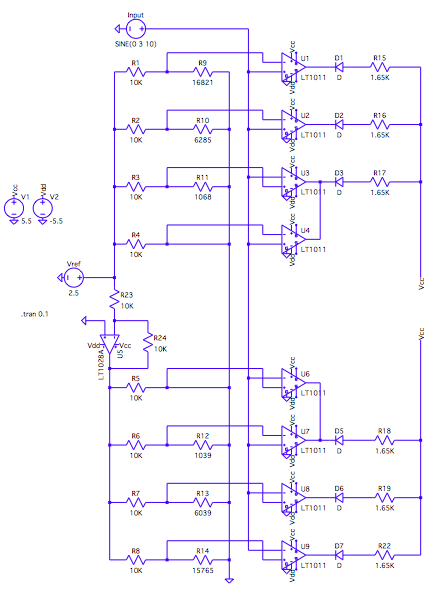
\includegraphics[scale=1.0]{figures/cProblemloesning/komparator_visuel1.PNG}
	\caption{Figuren illustrerer komparatorkonfigurationen for den visuelle del. Kredsløbet består af to dele; en for hældning i positiv retning og en for hældning i negativ retning. Hver del består af en vindues-komparator og to almindelige komparatorer. Der er implementeret en inverterende forstærker for at gøre referencespændingen negativ, så hældning i den negative retning kan dedekteres. Kredsløbet er udarbejdet i LTspice.}
	\label{fig:komparator_visuel}
\end{figure}

%%%%%%%%%%%%%%%%%%%%%%%%%%%%%%%%%%%%%%%%%%%%%%%%%%%%%%%%%%%%%%%

\noindent\textbf{Beregning af tærskelværdier og tilhørende R$1$-R$14$ modstande for aktivering af LED-dioder} \\
Inputsignalet fra forrige blok, tilpasningsblokken, ligger mellem -$2.9417$V og $3.0151$V jævnfør afsnit \ref{KomparatorAfs}, side\pageref{KomparatorAfs}. Jævnfør systemets funktionelle krav afsnit \ref{FunkKrav}, side \pageref{FunkKrav} ønskes det, at de enkelte LED-dioder skal lyse ved bestemte kropshældninger, dvs. ved en bestemt tærskelværdi. %Disse tærskelværdier sættes ud fra to punkter; det maksimale teoretiske signal  ved $25^{\circ}$ $4.0662$, og en tilgængelig spændingsreference, der kan sørge for en fast spænding til spændingstræet. 
Tærskelværdierne er udregnet til at være:

\begin{itemize}
\item $2^{\circ}$ = $0.2412$V
\item -$2^{\circ}$ = -$0.2353$V
\item $8^{\circ}$ = $0.9648$V
\item -$8^{\circ}$ = -$0.9413$V
\item $13^{\circ}$ = $1.5679$V
\item -$13^{\circ}$ = -$1.5297$V
\item $25^{\circ}$ = $3.0151$V
\item -$25^{\circ}$ = -$2.9417$V
\end{itemize}

\begin{figure}[H]
	\centering
	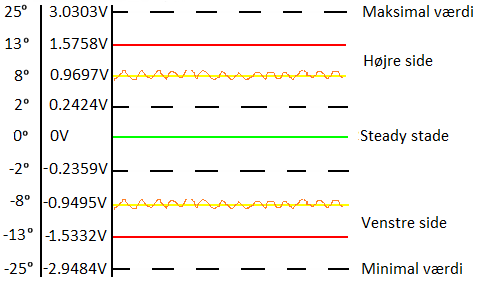
\includegraphics[scale=1.0]{figures/cProblemloesning/Taerskelvaerdier.PNG}
	\caption{Af figuren fremgår de beregnede tærskelværdier.}
	\label{fig:taerskelvaerdier}
\end{figure}

Der vælges en  spændingsreference, som består af en regulator så den kan levere $2.5$V til komparatorkredløbet. Spændingsreferencen indgår som del af en spændingsdeler og benyttes for at holde en fast referencespænding, da spændingen ved anvendelse af et batteri vil falde som funktion af tid. For at muliggøre anvendelsen af spændingsforsyningen på $2.5$V til negative tærskelværider benyttes en inverterende forstærker med et gain på $1$, der fremgår af figur \figref{fig:komparator_visuel}. Ved denne konfiguration vendes signalet uden at blive forstærket og kan på denne måde benyttes som referencespænding til negative inputspændinger.  
Når referencespændingen er kendt kan modstandene i spændingsdeleren bestemmes. Da kredsløbet trækker strøm har modstandene (R$15$-R$20$) til formål at sikre, at spændingsforsyningen ikke drænes. Hvis modstanden er høj, vil strømmen til kredsløbet være lav, og batterierne i spændingsreferencen vil derved holde længere.

Der anvendes otte spændingsdelere, hvor fire indgår som vindues-komparatorer og de resterende som almindelige komparatorer, hvillket fremgår af figur \figref{fig:komparator_visuel}.. 
For at opstille spændingsdelerne skal R$1$-R$14$ bestemmes så LED-dioderne lyser ved de ønskede tærskelværdier. For at modstandene kan bestemmes defineres R$1$ til en bestemt værdi, der her fastsættes til at være $10$K$\Omega$. Den samme værdi er gældende for R$2$-R$8$, eftersom der anvendes en spændingsdeler for hver tærskelværdi. Herefter kan R$9$-R$14$ udregnes vha. den generelle formel for en spændingsdeler jævnført \eqref{Spaendingsdeler}. Hvor følgende er kendt:
\begin{itemize}
\item $V_out$ = den ønskede tærskelværdi
\item $V_in$ = spændingsreferencen
\item R$1$-R$8$ = $10$K$\Omega$
\end{itemize}

Dette medfører at R$9$-R$14$ giver følgende resultater:\\
R$9$ = $16821\Omega$ \\
R$10$ = $6285\Omega$ \\
R$11$ = $1068\Omega$ \\
R$12$ = $1039\Omega$ \\
R$13$ = $6039\Omega$ \\
R$14$ = $15765\Omega$ \\

%%%%%%%%%%%%%%%%%%%%%%%%%%%%%%%%%%%%%%%%%%%%%%%%%%%%%%%%

\noindent\textbf{Beregning af R$15$-R$20$ modstande for aktivering af LED-dioder} \\
Jænvfør kravspecifikationerne i afsnit \ref{KomparatorAfs}, side \pageref{KomparatorAfs} for komparatoren skal forsyningsspændingen være $5.5$V. De anvendte LED-dioder i systemet er: to grønne L-$53$LG $5$mm (D$3$ og D$4$), to røde L-$53$LI $5$mm (D$1$ og D$6$) og to gule L-$53$LY $5$mm (D$2$ og D$5$). Disse LED-dioder kræver en minimum spænding på 2mA for at lyse og spændingsfaldet over LED-dioderne ligger maksimalt i intervallet $2.0$V til $2.2$ V (rød: $2.0$, gul: $2.1$ og grøn: $2.2$), men typisk mellem $1.7$V-$1.9$V. LED-dioderne skal derudover forsynes med $2$mA for at fungere, men kan forsynes med op til $150$mA, før de brændes af. LED-dioderne forsynes af en $5.5$V spændingsforsyning og tilkobles, som sagt, tilhørende modstande for bla. at undgå at LED-dioderne brænder af. Spændingsfaldet over dioderne samt den spænding LED-dioderne som minimum skal bruge for at lyse er kendte værdier, dvs. modstandene R$15$-R$20$ kan derfor findes vha. Ohms lov. Nedestående udregning giver en værdi af modstandene, hvis spændingsforsyningen giver $5.5$V til kredløbet og hvor der tages udgangspunkt i den minimale strøm for LED-dioderne:

\begin{equation}
R = \dfrac{5.5V - 2.2V}{2mA} = 1650\Omega
\end{equation}
\noindent Dermed sættes modstandene R$15$-R$20$ alle til $1650\Omega$ for at sikre, at der er tilstrækkeligt med strøm i kredsløbet til at dioderne kan lyse, uden at de brændes af eller at batterierne drænes. Opsætningen af LED-dioderne fremgår af figur \figref{fig:komparator_visuel}.

%%%%%%%%%%%%%%%%%%%%%%%%%%%%%%%%%%%%%%%%%%%%%%%%%%%%%%%%%%%
\noindent\textbf{Beregning af tærskelværdier og tilhørende R1-R5 modstande for aktivering af  vibratorerne} \\
Jævnfør kravsspecifikationerne i afsnit \ref{KomparatorAfs}, side \pageref{KomparatorAfs} skal vibratorerne have to tærskelværdier. For aktivering af vibratorerne anvendes derfor to komparatorer. Vibratorernes tærskelværdier konstrueres ligeledes vha. to parallelforbundede modstande og spændingsreferencer, samt de resterende modstande mellem vibratorerne og $+V_{cc}$. På figur X vises konstruktionen af kredsløbet med de to vibratorer og tilhørende modstande. \\

indsæt billede og word dokument \\

\noindent\textbf{Beregning af R6-R10 modstande for aktivering af vibratorerne} \\
Vibratorerne der anvendes i systemet er af typen XX... Afsnit skal skrives, når vi har information om vibratorer.  \\

FÅ SWITCH MED IND I DET? \\

\subsubsection{Simulering}
\noindent\textbf{Simulering af visuel komparatorkonfiguration} \\
Til simulering af den visuelle komparatorkonfiguration anvendes komparatorer af typen LT$1011$, da operationsforstærkerne til det reelle kredsløb er af denne type. For at udføre en simulering af den visuelle komparatorkonfiguration tilkobles kredsløbet et sinus-signal, der svinger mellem $\pm3$V. Dette gøres for at simulere signalet, der kommer fra den forrige blok, hvor arbejdsområdet er på $\pm3$V. Under simuleringen i LTspice testes det, hvorvidt den visuelle komparatorkonfiguration opfylder de opstillede specifikke krav, jævnfør kravspecifikationerne i afsnit \ref{KomparatorAfs}, side \pageref{KomparatorAfs}. Simuleringen af den visuelle komparatorkonfiguration fremgår af figur \figref{fig:komparator_visuel_simulering_samlet}. \fxnote{Vi kan starte med at simulere tærskelværdier og derefter hvordan komparatoren fungerer.}
\begin{figure}[H]
	\centering
	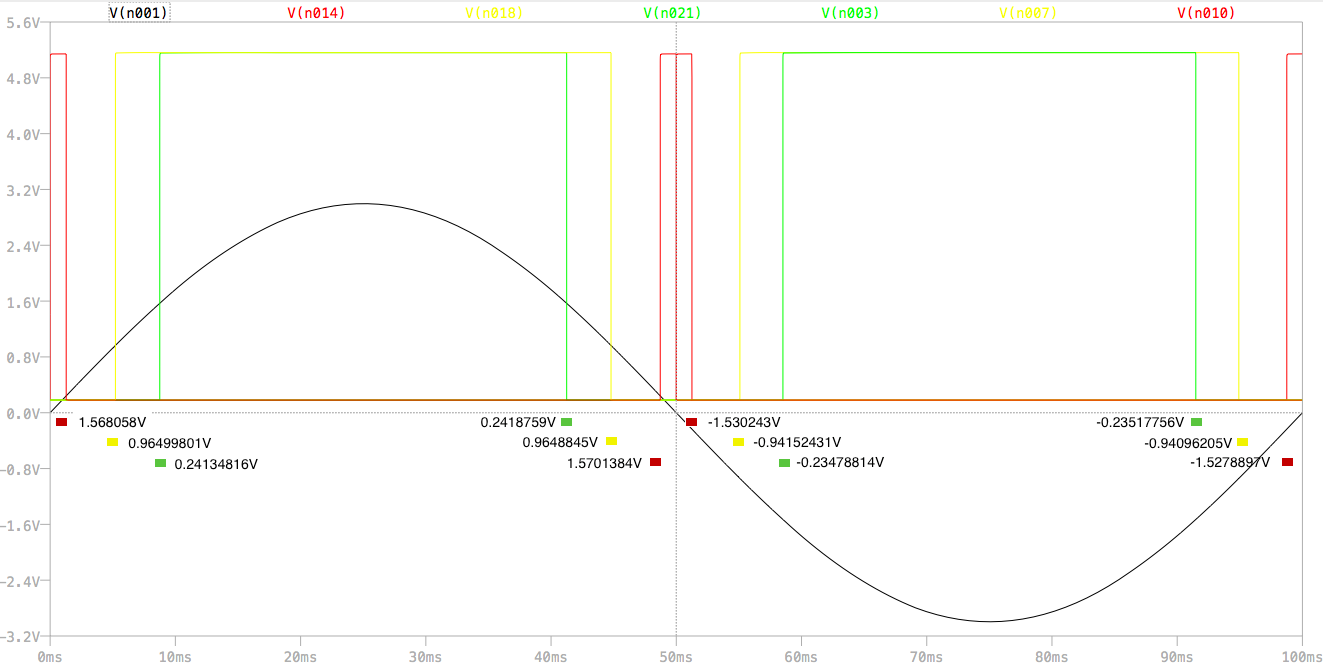
\includegraphics[scale=1.0]{figures/cProblemloesning/komparator_visuel_simulering_samlet1.PNG}
	\caption{Figuren viser simuleringen af den visuelle komparatorkonfiguration. Den sorte kurve er et sinus signal, der illustrerer blokkens inputsignal. De resterende kurver er de enkelte komparatorer, som under tærskelværdien er i negativ mætning. De røde kurver symboliserer den røde diode, de gule kurver de gule dioder og de grønne kurver de grønne dioder. Når inputsignalet når de definerede tærskelværdier, vil kurverne gå i positiv mætning og LED-dioderne vil lyse. Ved vindue-komparatoren er den positive og negative mætning ikke så høj, som ved de normale komparatorer. Dette skyldes, at signalet skal passere yderligere to LED-dioder, hvilket giver et spændingsfald. Kredsløbet er simuleret i LTspice.}
	\label{fig:komparator_visuel_simulering_samlet}
\end{figure}
På figur \figref{fig:komparator_visuel_simulering_samlet} fremgår det, at ved de enkelte tærskelværdier går signalet i positiv mætning, hvilket får LED-dioderne til at lyse. Mætningen er under $5.5$V som er den spænding LED-dioderne maksimalt kan forsynes med  \fxnote{Kontrollere af denne værdi (5.5) er rigtig}, men samtidig nok til at få dioderne til at lyse, hvilket krævede mellem $1.7-1.9$V og $2$mA. 

\begin{table}[H]
	\centering
	\begin{tabular}{|l|l|l|l|l|l|}
		\hline
					& \textit{Tærskelværdier} 	& \textit{Måling til højre} & \textbf{Måling til venstre}		&  \textit{Afvigelse for højre}  \textit{Afvigelse for venstre}\\ \hline
\textbf{$2^{\circ}$} 		& $0.2412$V  				&$0.24134816$V 			&$0.24118759$V		& $0.06\%$  &$0.005\%$ \\ \hline
\textbf{-$2^{\circ}$} 		&-$0.2353$V 					&-$0.23478814$V 			&-$0.23517756$V  	& $0.2\%$	&$0.05\%$\\ \hline
 \textbf{$8^{\circ}$} 		&$0.9648$V					&$0.96499801$V			&$0.9648845$V		& $0.02\%$	&$0.009\%$\\ \hline
\textbf{-$8^{\circ}$} 		&-$0.9413$V					&-$0.94152431$V 			&-$0.94096205$V		& $0.02\%$	&$0.04\%$\\ \hline 		
\textbf{$13^{\circ}$} 		&$1.5679$V 					&$1.5680858$V 		  	&$1.5701384$V		& $0.01\%$	&$0.14\%$\\ \hline
\textbf{-$13^{\circ}$} 		&-$1.5297$VV 				&-$1.530243$V		   	&-$1.5278897$V		& $0.04\%$	&$0.12\%$ \\ \hline
	\end{tabular}
	\caption{I tabellen ses der, at de anvendte tærskelværdier afviger fra den teoretiske værdi, hvilket er forventet af reelle komponenter. Det er en acceptabel afvigelse, så tærskelværdierne kan derfor anvendes til implementering}
	\label{Tab:Maalingtearskelvaerdier}
\end{table}

Det kan udfra \ref{Tab:Maalingtearskelvaerdier} konkluderes at afvigelsen fra de udregnede tærkselværdier stemmer overens med tolerance for tærkselværdierne jævnfør afsnit \ref{KomparatorAfs}, side \pageref{KomparatorAfs} som var på $\pm1$\%. 

\noindent\textbf{Simulering af somasensorisk komparator kredsløb} \\

\subsubsection{Implementering og test}

\subsection{Feedback - Visuel}
\subsubsection{Teori og design}
\subsubsection{Simulering}
\subsubsection{Implementering og test}
%%%%%%%%%%%%%%%5
\subsection{Feedback - Somatosensorisk}
\subsubsection{Teori og design}
\subsubsection{Simulering}
\subsubsection{Implementering og test}

%\subsection{Feedback}
%%%%%%%%%%%%%%%%%%%%%%%%%%%
%\subsubsection{Visuel Feedback}
%\textbf{Teori og design} \\
%\noindent .. \\
%\textbf{Simulering} \\
%\noindent .. \\
%\textbf{Implementering og test} \\
%\noindent ..
%%%%%%%%%%%%%%%%%%%%%%%%%%%
%\subsubsection{Somatosensorisk Feedback}
%\textbf{Teori og design} \\
%\noindent .. \\
%\textbf{Simulering} \\
%\noindent .. \\
%\textbf{Implementering og test} \\
%\noindent .. \\
% !TeX spellcheck = da_DK
\subsection{Spændingsforsyning} \label{Spaendingsforsying}
\subsubsection{Teori og design}
Til systemet anvendes to $1.5$V batterier som spændingsforsyning, der placeres i en spændingsregulator. Denne kan teoretisk og reelt levere en spænding på hhv. $\pm5.5$V og $3.4$V fra to forskellige terminaler. Derudover besidder spændingsregulatoren en jordkobling, som øvrige komponenter i systemet kan tilkobles. Til dette system benyttes begge terminaler; $3.4$V forsyner vibratorerne, og $\pm5.5$V benyttes til resten af systemet. Spændingsregulatoren er designet således, at den leverer en spænding koblet i en split-supply.\\%Den positive pol fra det ene batteri tilkobles den negative pol på det andet batteri i. Derudover dannes en fælles jordforbindelse for øvrige komponenter i systemet, som kræver en forbindelse til jord. Den negative pol i det første batteri i det første batteri anvendes som systemets negative forsyningsspænding og indikeres med $-V_{cc}$, mens det andet batteri anvendes som den positive spændingsforsyning og indikeres med $+V_{cc}$.
Da batterierne ikke leverer den samme spænding gennem deres levetid, skal disse skiftes ud, når de ikke leverer den nødvendige spænding til systemet. Batteriernes levetid afhænger af, hvor meget strøm systemet bruger. %Da komparatorkonfigurationen kræver den højeste spænding iblandt blokkene, skal spændingsregulatoren minimum leverer en spænding på xx V. Derfor kræver systemt en minimal spænding på xx V.

\subsubsection{Simulering}
Ved simulering af spændingsforsyningen anvendes LTspice, hvor der sendes en spænding igennem en buffer, som også er beskrevet og benyttet i bilag \ref{Bilag:Pilotforsoeg}, side \pageref{Bilag:Pilotforsoeg}. Herved kan konsekvensen af et faldende input simuleres, således at kravene undersøges, jævnfør afsnit \ref{Krav_spaending_spicifikt}, side \pageref{Krav_spaending_spicifikt}. Det maksimale input, som ledes gennem systemet uden der ønskes klipning af signalet, er:
\begin{equation}
0.0037 \cdot 9.1 \cdot 3.6 \cdot 25 = 3.0303
\end{equation}
\indent Denne spænding benyttes i simuleringen som amplituden på et sinussignal. Konsekvensen af en faldende spændingsforsyning undersøges, hvilket er illustreret på \figref{fig:spaendingsforsyning_graf}. Der forsynes med hhv. $\pm5.5$V, $\pm5$V, $\pm4.5$V og $\pm4$V.
\begin{figure}[H]
	\centering
	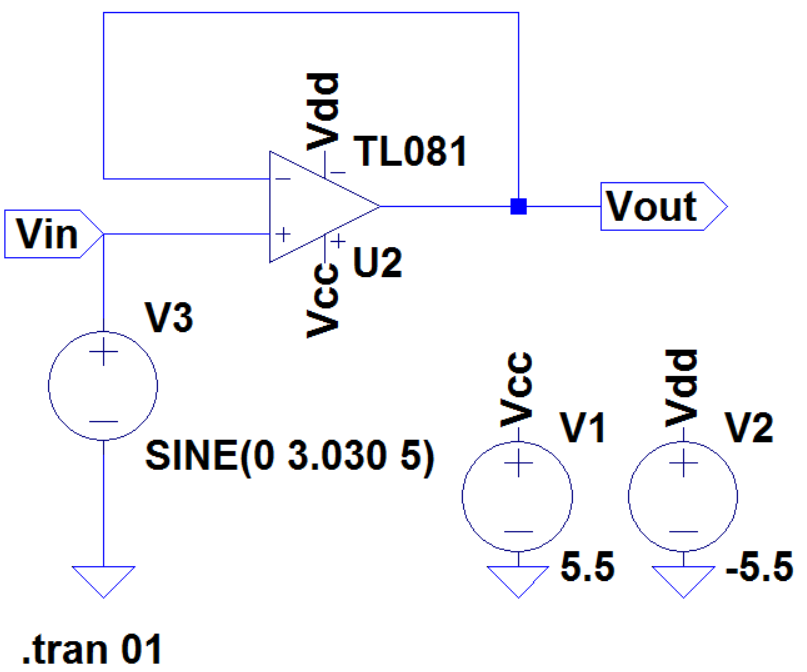
\includegraphics[scale=0.4]{figures/cProblemloesning/Spaendingsforsyning_LTspice2.PNG}
	\caption{På figuren ses designet af spændingsforsyningen med en buffer. Inputsignalet er en sinuskurve med en amplitude på det maksimalt ønskede signal i systemet. Spændingsforsyningen til operationsforstærkeren er på billedet $\pm5.5$V, hvilket er den spænding, som anvendes til at forsyne systemet.}
	\label{fig:spaendingsforsyning}
\end{figure}
\begin{figure}[H]
	\centering
	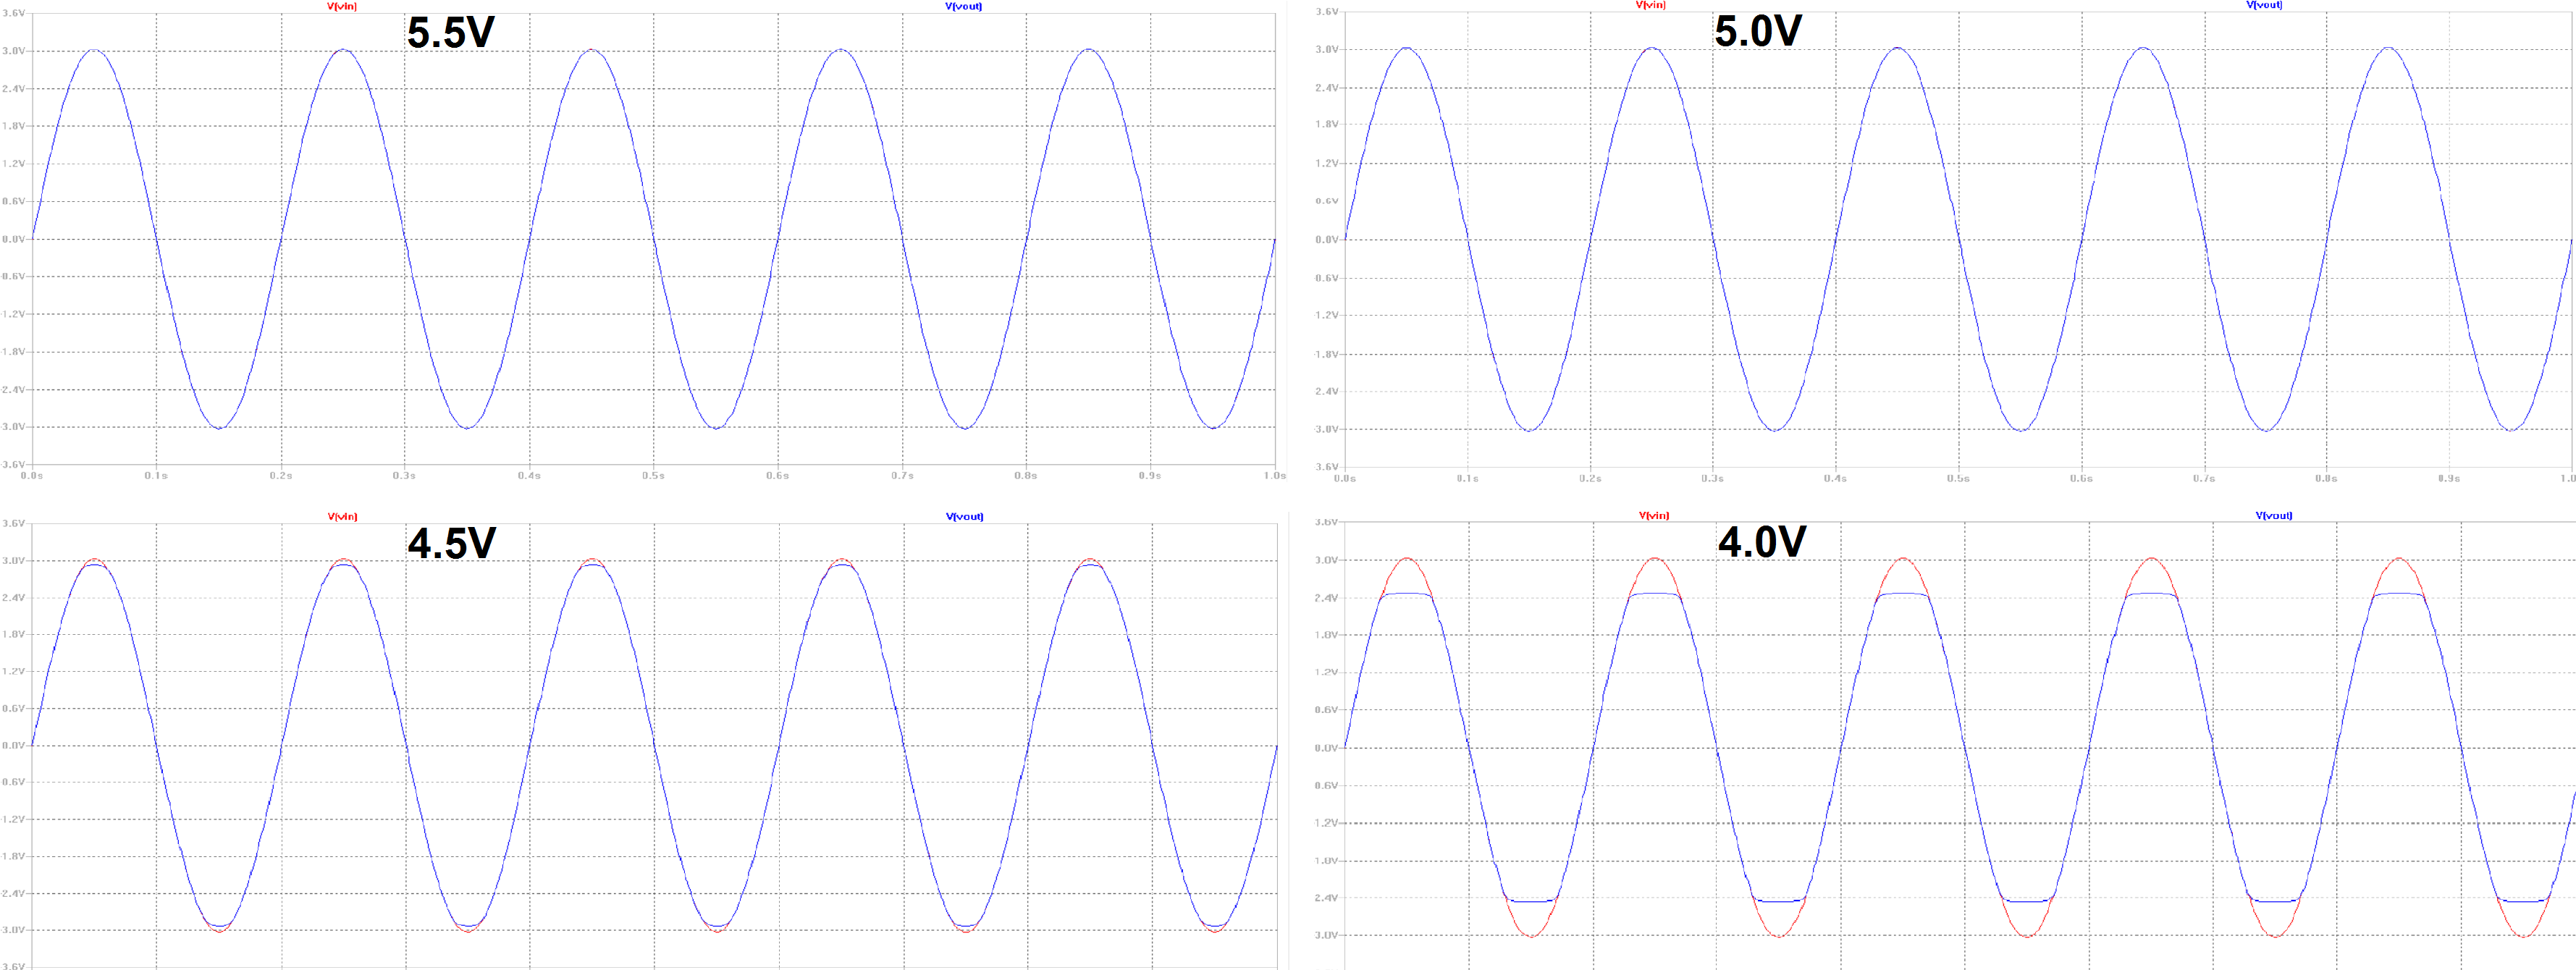
\includegraphics[scale=0.17]{figures/cProblemloesning/Spaendingsforsyning2.PNG}
	\caption{På figuren ses simuleringen af en spændingsforsyning på hhv. $\pm5.5$V, $\pm5$V, $\pm4.5$V og $\pm4$V. Det fremgår af figuren, at signalet klippes ved $4.5$V, hvilket ses tydeligere, når spændingsforsyningen sænkes til $4.0$V.}
	\label{fig:spaendingsforsyning_graf}
\end{figure}
\noindent På \figref{fig:spaendingsforsyning_graf} ses simuleringen af systemet ved fire forskellige spændingsforsyninger. Der ses, at signalet ideelt vil blive klippet, hvis spændingsforsyningen leverer under $5.0$V til operationsforstærkerne.

\subsubsection{Implementering og test}
Det undersøges, hvorvidt spændingsregulatoren leverer en spænding på mindst $\pm5.5$V samt $3.4$V fra hver terminal, jævnfør afsnit \ref{Krav_spaending_spicifikt}, side \pageref{Krav_spaending_spicifikt}. Derudover testes det, om spændingsregulatoren kan forsyne samtlige blokke i systemet med den minimalt krævede spænding samt forsyner operationsforstærkerne med mindst $5.0$V for at undgå klipning af signalet. \\
Batterierne blev inden testen målt til henholdsvis $1.5394$V og $1.5373$V. Jævnfør afsnit \ref{Krav_spaending_spicifikt}, side \pageref{Krav_spaending_spicifikt} accepteres en spænding under $5.5$V ikke, hvorimod der accepteres en afvigelse på $\pm10\%$ for $3.4$V. Derfor vil afvigelserne for spændingsforsyningen på $\pm5.5$V angives i V, hvorimod afvigelsen for $3.4$V angives i procent.
\begin{table}[H]
	\centering
	\begin{tabular}{|l|l|l|}
		\hline
		\textit{Teoretisk} & \textit{Målt} & \textit{Afvigelse} \\ \hline
		$\pm5.5$V          &     \begin{tabular}[c]{@{}l@{}}$5.5643$V\\-$5.5766$V\end{tabular} & \begin{tabular}[c]{@{}l@{}}$0.0643$V\\$0.0766$V\end{tabular}        \\ \hline
		$3.4$V             &     $3.3746$V                 &      $0.75\%$                                \\ \hline
	\end{tabular}
	\caption{I tabellen ses outputtet fra spændingsregulatoren, når den ikke er koblet til det samlede kredsløb.}
	\label{tab:spaending_resultat}
\end{table}
 
\begin{table}[H]
	\centering
 	\begin{tabular}{l|l|l|l|}
 		\cline{2-4}                                                                                                                                      & \textit{Teoretisk} & \textit{Målt}                                                  & \textit{Afvigelse}                                              \\ \hline
 		\multicolumn{1}{|l|}{\textit{\begin{tabular}[c]{@{}l@{}}Spændingsforsyning\\ til accelerometer\end{tabular}}}                          & $\pm5.5$V          & $5.5315$V                                                      & $0.0315$V                                                      \\ \hline
 		\multicolumn{1}{|l|}{\textit{\begin{tabular}[c]{@{}l@{}}Spændingsforsyning\\ til offsetjustering\end{tabular}}}                        & $\pm5.5$V          & \begin{tabular}[c]{@{}l@{}}$5.5386$V\\ -$5.5530$V\end{tabular} & \begin{tabular}[c]{@{}l@{}}$0.0386$V\\ $0.0530$V\end{tabular} \\ \hline
 		\multicolumn{1}{|l|}{\textit{\begin{tabular}[c]{@{}l@{}}Spændingsforsyning til \\ referencespænding til offsetjustering\end{tabular}}} & $\pm5.5$V          & \begin{tabular}[c]{@{}l@{}}$5.5384$V\\ -$5.5528$V\end{tabular} & \begin{tabular}[c]{@{}l@{}}$0.0384$V\\ $0.0528$V\end{tabular} \\ \hline
 		\multicolumn{1}{|l|}{\textit{\begin{tabular}[c]{@{}l@{}}Inputspænding til \\ referencespænding til offsetjustering\end{tabular}}}      & $\pm5.5$V          & $5.5320$V                                                      & $0.0320$V                                                      \\ \hline
 		\multicolumn{1}{|l|}{\textit{\begin{tabular}[c]{@{}l@{}}Spændingsforsyning\\ til faktor $9.1$ forstærker\end{tabular}}}                & $\pm5.5$V          & \begin{tabular}[c]{@{}l@{}}$5.5308$V\\ -$5.5526$V\end{tabular} & \begin{tabular}[c]{@{}l@{}}$0.0308$V\\ $0.0526$V\end{tabular} \\ \hline
 		\multicolumn{1}{|l|}{\textit{\begin{tabular}[c]{@{}l@{}}Spændingsforsyning\\ til filter\end{tabular}}}                                 & $\pm5.5$V          & \begin{tabular}[c]{@{}l@{}}$5.5374$V\\ -$5.5292$V\end{tabular} & \begin{tabular}[c]{@{}l@{}}$0.0374$V\\ $0.0292$V \end{tabular} \\ \hline
 		\multicolumn{1}{|l|}{\textit{\begin{tabular}[c]{@{}l@{}}Spændingsforsyning\\ til faktor $3.6$ forstærker\end{tabular}}}                & $\pm5.5$V          & \begin{tabular}[c]{@{}l@{}}$5.5378$V\\ -$5.5293$V\end{tabular} & \begin{tabular}[c]{@{}l@{}}$0.0378$V\\ $0.0293$V\end{tabular} \\ \hline
 		\multicolumn{1}{|l|}{\textit{\begin{tabular}[c]{@{}l@{}}Spændingsforsyning til\\ komparatorblokken\end{tabular}}}                      & $\pm5.5$V          & \begin{tabular}[c]{@{}l@{}}$5.5358$V\\ -$5.5302$V\end{tabular} & \begin{tabular}[c]{@{}l@{}}$0.0373$V\\ $0.0302$V\end{tabular} \\ \hline
 		\multicolumn{1}{|l|}{\textit{\begin{tabular}[c]{@{}l@{}}Spændingsforsyning til \\ referencespænding til feedbackkonfigurationen\end{tabular}}} & $\pm5.5$V          & \begin{tabular}[c]{@{}l@{}}$5.5373$V\\ $-5.5302$V\end{tabular} & \begin{tabular}[c]{@{}l@{}}$0.0373$V\\ $0.0302$V\end{tabular} \\ \hline
 		\multicolumn{1}{|l|}{\textit{\begin{tabular}[c]{@{}l@{}}Inputspænding til \\ referencespænding til feedbackkonfigurationen\end{tabular}}}    & $\pm5.5$V          & $5.5373$V                                                      & $0.0373$V                                                      \\ \hline
 		\multicolumn{1}{|l|}{\textit{\begin{tabular}[c]{@{}l@{}}Spændingsforsyning til\\ vibratorer - før Schottky-diode\end{tabular}}}         & $3.4$V             & $3.3740$V                                                      & $0.76\%$                                                        \\ \hline
 	\end{tabular}
  	\caption{I tabellen ses forsyningen eller inputspænding blokkene i systemet.}
  	\label{tab:spaending_systemet}
\end{table}
\noindent I \tableref{tab:spaending_resultat} og \textbf{\ref{tab:spaending_systemet}} ses det, at spændingsregulatoren har en afvigelse på $0.75\%$ ift. $3.4$V spændingen. Derudover leverer den mindst $\pm5.5$V, når spændingsregulatoren ikke er tilkoblet systemet. Efter tilkobling ses det i \tableref{tab:spaending_systemet}, at spændingsregulatoren forsyner blokkene i systemet med den minimale spænding, som er krævet for korrekt funktion. Det vides fra teorien og kan ses i simuleringen, at så længe spændingsforsyningen leverer mindst $\pm5$V, vil den ikke forårsage klipning af signalet. Hvis forsyningen på teoretisk $3.4$V leverer under dette, vil det have en indvirkning på vibratorernes funktion, da det kun er disse, $3.4$V spændingen benyttes til at forsyne. \\
Da samtlige afvigelser ligger indenfor tolerancerne, jævnfør afsnit \ref{Krav_spaending_spicifikt}, side \pageref{Krav_spaending_spicifikt}, accepteres spændingsforsyningen.
% !TeX spellcheck = da_DK
\subsection{ADC}\label{ADC_afsnit}
\subsubsection{Teori og design}
I dette projekt anvendes en ADC af typen NI USB-6009 til at konvertere det analoge signal til digital som beskrevet i afsnit \ref{ADCafsnit} på side \pageref{ADCafsnit}. %Signalet skal konverteres, for at kunne sendes ind i den digitale del af systemet, så plejepersonalet kan aflæse og behandle målingerne. 
Med denne ADC kan der samples med $13$ bits single-ended\fxnote{Hvad betyder det?}. ADC'en kan dermed inddeles i $2^{13} = 8192 \text{niveauer}$. Den maksimale sampling rate er på $48$kS/s, hvormed det er muligt at sample med minimum det tidobbbelte af båndbredden. Arbejdsområdet for ADC'en ift. spænding ligger på $10Vpp$ og har en typisk præcision på $14.7$mV ved $25^{\circ}$C. \cite{Instruments2014} Ud fra oplysningerne er det muligt at udregne LSB ud fra ligningen i afsnit \ref{ADCafsnit} på side \pageref{ADCafsnit}. Udregningen ser således ud: \\
\begin{equation}
	LSB = \frac{FSR}{2^{n}} 
\end{equation}  
FSR er arbejdsområdet, dvs. $10Vpp$, som indsættes i formlen som $20V$, imens n er antallet af bits, der kan samples med, dvs. $13$.
Værdierne indsættes i formlen: \\
\begin{align}
	LSB = \frac{20V}{2^{13}}
	LSB = 0.00244V = 2.44\text{mV}
\end{align}
Det opsamlede signal bliver forvrænget, og vil dermed ikke være repræsentativt, hvis der opsamles værdier på under $2.44mV$.\\
\subsubsection{Simulering}
Ifølge tolerancerne for ADC'en beskrevet i afsnit \ref{ADCafsnit} på side \pageref{ADCafsnit} skal der testes, om ADC'en kan modtage og konvertere et inputsignal på $\pm4$V samt sample 500 gange i sekundet. \\
Der kan ikke laves en simulering af en ADC i programmet LTSpice, da inputsignalet i LTSpice allerede er et digitalt signal, og der er derfor ikke noget, som skal konverteres.
 
\subsubsection{Implementering og test}
ADC'en skal implementeres og tilkobles efter lavpasfiltret, som det kan ses på \figref{kravblok} på side \pageref{kravblok}. \\
Der benyttes en tonegenerator til at undersøge, om den valgte ADC overholder kravene beskrevet i afsnit \ref{ADCafsnit} på side \pageref{ADCafsnit}. Tonegeneratoren skal sende fem forskellige input til ADC'en;
\begin{enumerate}
	\item Et sinussignal med en frekvens på $100$Hz og den højeste forventede amplitude, dvs. $3.0147 \times 2 = 6.0294\text{Vpp}$.
	\item Et sinussignal med en frekvens på $100$Hz og den laveste forventede amplitude, dvs. -$2.9400 \times 2 = -5.8800 \approx 5.8800\text{Vpp}$.
	\item Et sinussignal med en frekvens på $25$Hz og en amplitude på $8$Vpp, da der ses i \tableref{Tab:faktor3_test}, at operationsforstærkerne går i mætning ved ca. $4$V, når de forsynes med $5.5$V. 
	\item Et sinussignal med en frekvens svarende til knækfrekvensen i lavpasfiltret, dvs. $25$Hz, og den højeste forventede amplitude, dvs. $3.0147 \times 2 = 6.0294\text{Vpp}$.
	\item Et sinussignal med en frekvens svarende til knækfrekvensen i lavpasfiltret, dvs. $25$Hz, og den laveste forventede amplitude, dvs. -$2.9400 \times 2 = -5.8800 \approx 5.8800\text{Vpp}$.
\end{enumerate}
Der samples med $500$Hz, selvom $250$Hz havde været nok, da vores båndbredte er $25$Hz, men ScopeLogger kan enten sample med $200$ eller $500$, så derfor samples der med $500$Hz. På \figref{fig:ADC_Test} ses resultatet af målingerne.

\begin{figure}[H]
	\centering
	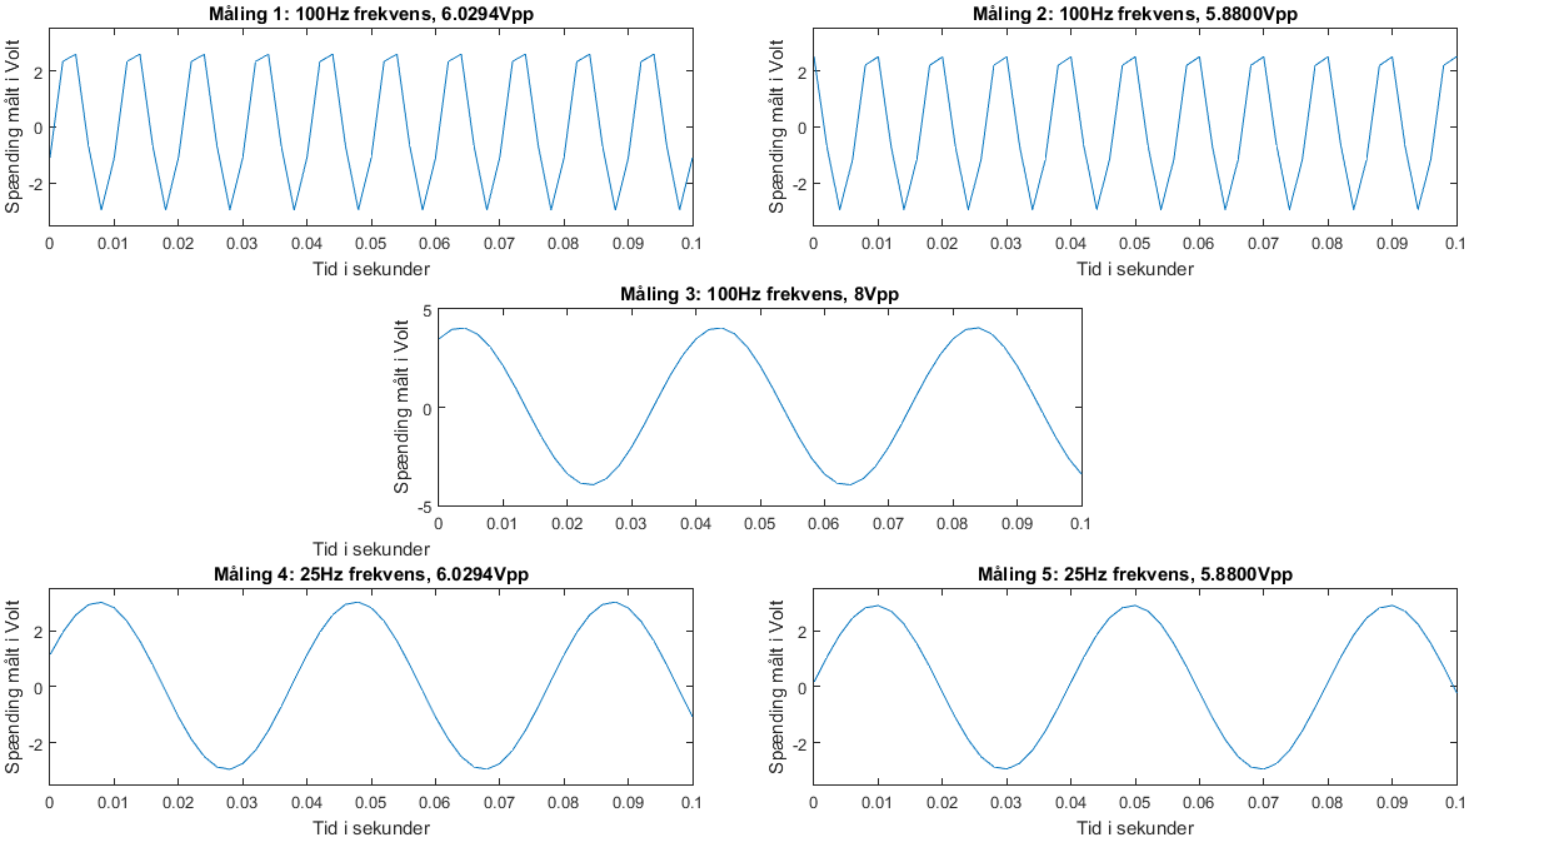
\includegraphics[scale=0.45]{figures/cProblemloesning/ADC_Test2_matlab.PNG}
	\caption{På figuren ses resultatet af de fem målinger plottet i Matlab. Overskiften til hver graf beskriver amplituden og frekvensen for signalet i hver måling. Der ses, at x-aksen for alle plots er sat til 0.1 sekunder.}
	\label{fig:ADC_Test}
\end{figure}

\noindent Dataen optaget med ADC'en, som er plottet i \figref{fig:ADC_Test}, blev efterfølgende bearbejdet i Matlab. Derudover blev et oscilloskop tilkoblet outputtet fra tonegeneratoren. Resultatet herfra betragtes som det faktiske output fra tonegeneratoren, hvilket indgår i beregningen af afvigelsen i ADC'ens sampling. Resultaterne ses i \tableref{Tab:ADC_resultat}:

\begin{table}[H]
	\centering
	\begin{tabular}{|l|l|l|l|l|l|}
		\hline
		\textit{Måling nr} & \textit{\begin{tabular}[c]{@{}l@{}}Indstillet\\ frekvens\end{tabular}} & \textit{\begin{tabular}[c]{@{}l@{}}Indstillet\\ amplitude\end{tabular}} & \textit{\begin{tabular}[c]{@{}l@{}}Målte amplitude\\ på oscilloscop\end{tabular}} & \textit{\begin{tabular}[c]{@{}l@{}}Målte amplitude\\ via ADC\end{tabular}} & \textit{Afvigelse} \\ \hline
		\textit{$1$}         & $100$Hz     & $3.0147$V    & $3.0800$V      & $2.5989$V       & $15.62$\%          \\ \hline
		\textit{$2$}         & $100$Hz     & $2.9400$V    & $2.9200$V      & $2.5284$V       & $13.32$\%          \\ \hline
		\textit{$3$}         & $25$Hz      & $4$V         & $4.0400$V      & $4.0442$V       & $0.10$\%           \\ \hline
		\textit{$4$}         & $25$Hz      & $3.0147$V    & $3.0800$V      & $3.0689$V       & $0.36$\%           \\ \hline
		\textit{$5$}         & $25$Hz      & $2.9400$V    & $2.9200$V      & $2.9207$V       & $0.02$\%           \\ \hline
	\end{tabular}
	\caption{I tabellen ses resultaterne af det målte signal med hhv. et oscilloskop og ADC'en. Oscilloskopets måling betegnes som det korrekte og derved kan afvigelserne beregnes.}
	\label{Tab:ADC_resultat}
\end{table}

Der kan ses på \figref{fig:ADC_Test}, at sinussignalet i måling $1$ og $2$ er mere kantet end signalerne i måling $3$-$5$. Årsagen til dette kan være, at vi sampler med $500$Hz, mens signalets frekvens er $100$Hz. Dette gør, at ADC'en sampler med $5$ gange pr. periode og derved bliver signalet kantet. Derfor giver ADC'ens værdi for amplituden en procentafvigelse på henholdsvis $15.62$ og $13.32$, da der ikke samples med nok ift. frekvensen. Det vurderes dermed, at det er samplingsfrekvensen, som er årsagen til de høje afvigelser.\\
I måling $3$-$5$ er sinussignalets frekvens nedsat, hvilket gør, at signalet bliver mere regelmæssigt. Der samples med en samplingshastighed, der er $20$ gange større end frekvensen, og der opsamles derved tilstrækkeligt med datapunkter. Derfor er procentafvigelserne fra måling $3$-$5$ mere repræsentative for ADC'ens afvigelse. Men afvigelserne kan også skyldes afvigelser i oscilloskopet. Der vurderes derfor, at ADC'en viser det forventede og er dermed godkendt.
% !TeX spellcheck = da_DK
\subsection{USB-isolator}
Efter konvertering fra analogt til digital anvendes en USB-isolator til adskillelse af computeren til systemet samt sikre computerens forbindelse til elnettet. 
Der anvendes USB-isolatoren USI-01 som er godkendt til brug ved sikkerhedsklassifikation BF og CE som isoleringsspænding på 4kV samt fungerer som en galvanisk adskillende af systemet, hvilket har til formål at overføre signal mellem to isolerede kredsløb. For yderligere sikring af computerens forbindelse til elnettet er denne ikke tilkoblet elnettet. USB-isolatoren implementeres mellem ADC'en og computeren, hvilket er illustreret på \figref{blokdiagram} på side \pageref{blokdiagram}

\subsubsection{Test}
For at kunne teste, hvor vidt kravet jævnført \pageref{kravspecifikationer} om inputspændingen er lig med outputspændingen udføres en test, hvor dette sammenlignes. Dette gøres ved at tilslutte NIDAQ til USB-isolatoren til en spændingsforsyning og computer, som sammenligner inputspændingen med outputspændingen. Derudover indsættes et oscilloskop ved inputtet fra spændingsforsyning, som har til formål at måle den reelle spænding der løber fra spændingsforsyningen. 

\subsubsection{Resultat fra test}
De målte værdier fra testen ses i \figref{USBisolatortest}. Ud fra de målte værdier er der en afvigelse fra spændingsforsyningen til den målte værdi fra oscilloskop og ScopeLogger. De målte værdier fra ocilloskoppet er rent teoretisk de værdier som spændingsforsyningen vil give som input til kredsløbet. Der er en afvigelse fra 0\% til 1,5\% i forhold til spændingsforsyning og ocilloskoppet, dette kan skyldes at spændingsforsyningen har en tolerance i forhold til databladet for den enkelte spændingsforsyning. I forhold til spændingsforsyningen og Scopelogger er der en afvigelse fra -0,6\% til 0,3\%. En af grundene til denne forskel kan være at de reelle komponenter og systemet bruger en del af spændingen. Generelt varierer de anvendte instrumenter i antallet af decimaler på det visuelle skærm, hvilket ydermere kan være en faktor for at de målte værdier afviger fra det teoretiske. På baggrund af de målte værdier vurderes ud fra \pageref{kravspecifikationer} at USB-isolatoren må have en tolerance på $\pm$ 2\%.

\begin{center}
\label{USBisolatortest}
    \begin{tabular}{ | p{2cm} | p{2cm} | p{3.5cm} | p{2.1cm} | p{3.5cm} |}
    \hline
    \textbf{Spændings- forsyning} 	&  \textbf{Oscilloskop} 	& \textbf{\%-afvigelse for spændingsforsyning og oscilloskop}	& \textbf{ScopeLogger}	&\textbf{\%-afvigelse for spændingsforsyning og ScopeLogger} \\ \hline
    1,00V             				& 1,00V    				& 0,0\% 		    	& 0,9940V       &  -0,6006 \%  \\ \hline
    2,00V                          	& 2,03V					& 1,5\%			& 2,0237V       &   1,1827 \%  \\ \hline
    3,00V                         	& 3,03V					& 1,0\%	    		& 3,0060V       &   0,2008 \%   \\ \hline
    4,00V                          	& 4,06V					& 1,5\%			& 4,0131V       &   0,3280 \%   \\ \hline
    5,00V                          	& 5,06V					& 1,2\% 		& 5,0053V       &   0,1061 \%  \\ \hline
    \end{tabular}
\end{center}

\section{Software}
% !TeX spellcheck = da_DK
\section{Samlet systemtest}
Efter de enkelte blokke blev testet og godkendt hver for sig, skal det samlede system testes. Formålet med den samlede systemtest er at kontrollere, hvorvidt systemet overholder de overordnede funktionelle krav jævnfør afsnit \ref{FunkKrav} på side \pageref{FunkKrav}. Der anvendes samme fremgangsmåde for test af det samlede system, som af de øvrige blokke; Først simuleres systemet i LTspice, hvorefter det implementeres og testes.

\subsection{Simulering}
I simuleringen af det samlede system kontrolleres det, som i de øvrige simuleringer, om systemet fungerer med ideelle komponenter. Denne kontrol udføres ved at indsende en sinus som inputspænding igennem systemet, som teoretisk skal aktivere hhv. de enkelte dioder og vibratorerne. Designet af det samlede system ses på \figref{fig:samlet_system}:
\begin{figure}[H]
	\centering
	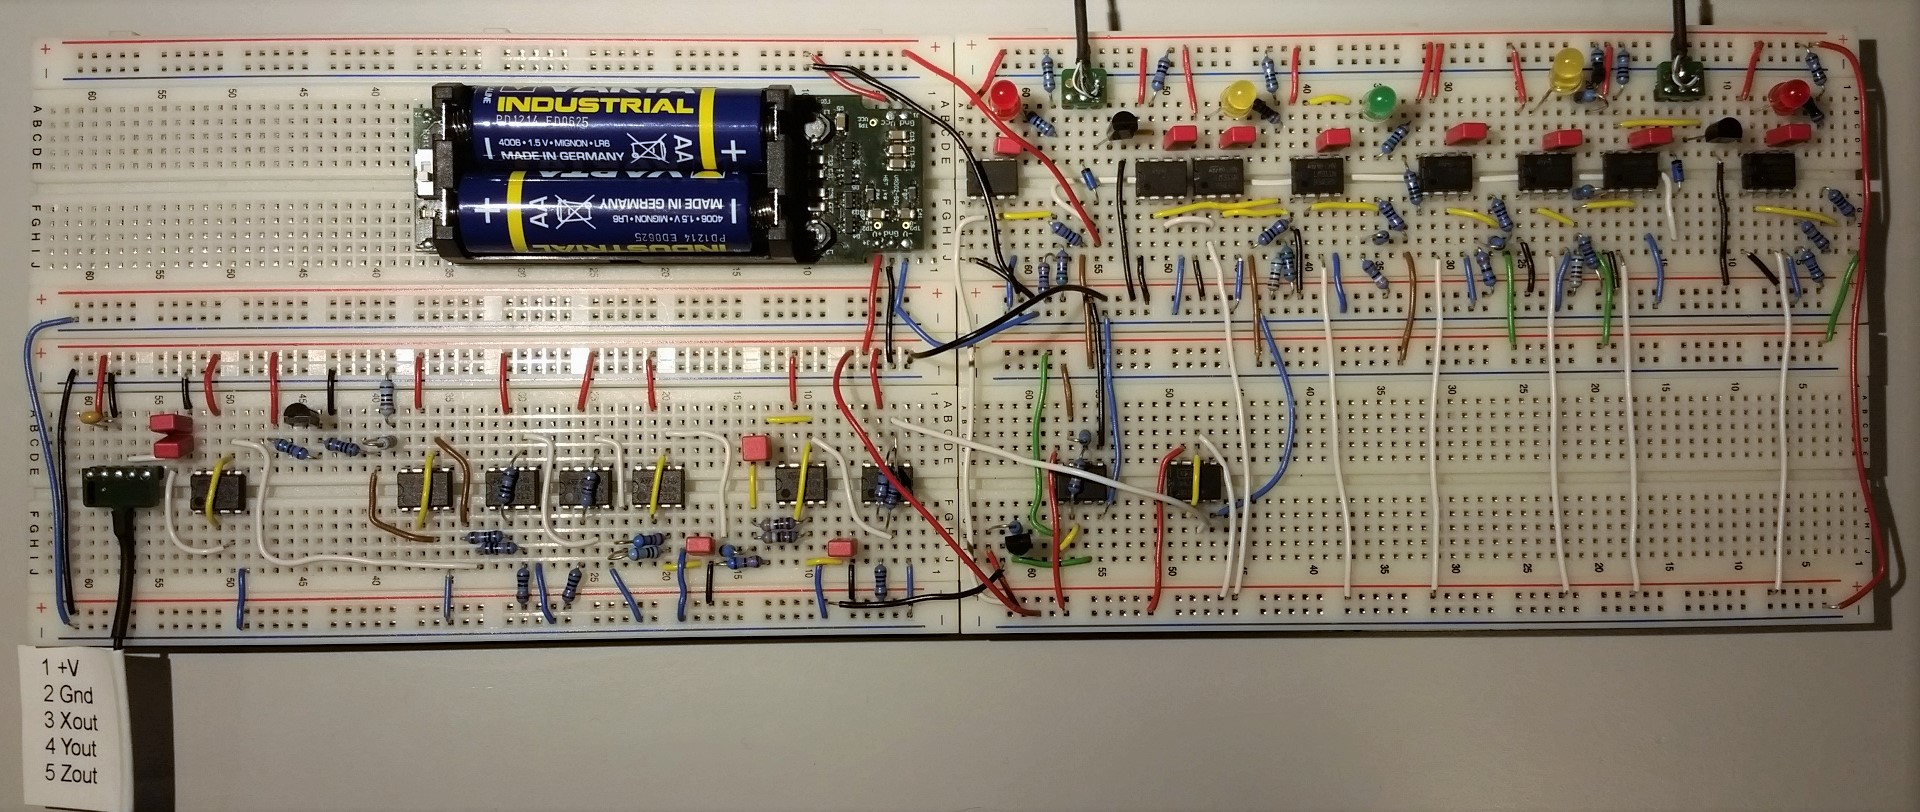
\includegraphics[scale=.38]{figures/cProblemloesning/Samlet_system2.PNG}
	\caption{På figuren ses designet af det samlede system med labels, der indikerer målepunkterne for de følgende simuleringer. Derved kan blokkenes påvirkning af signalet følges undervejs i systemet.}
	\label{fig:samlet_system}
\end{figure}
\noindent Sinussignalets amplitude udregnes til at være:
\begin{eqnarray}
0.0037 \cdot (\dfrac{(25-13)}{2} + 13) = 0.0703V
\end{eqnarray}
$0.0037$V er den maksimale spænding fra accelerometret ved $1^{\circ}$ hældning. Dette ganges med $19$, hvilket er midterpunktet for aktivering af en rød diode ($13^{\circ}$) og mætning af den sidste forstærker ($25^{\circ}$). Der fås en amplitude på $0.0703$V. Det kan derved måles, om systemet teoretisk opfylder de overordnede funktionelle krav jævnfør afsnit \ref{FunkKrav} på side \pageref{FunkKrav}.\\
I simuleringen af dette system måles inputtet fra accelerometret og outputtet for hver af feedback komponenterne. Dette ses på \figref{fig:samlet_system_simulering}:
%\begin{figure}[H]
%	\centering
%	\includegraphics[scale=.3]{figures/cProblemloesning/Samlet_system_simulering.PNG}
%	\caption{...}
%	\label{fig:samlet_system_simulering}
%\end{figure}

\subsection{Implementering og test}
Det samlede system implementeres på to breadboards. Opsætningen kan ses på \figref{fig:samlet_system_real}
\begin{figure}[H]
	\centering
	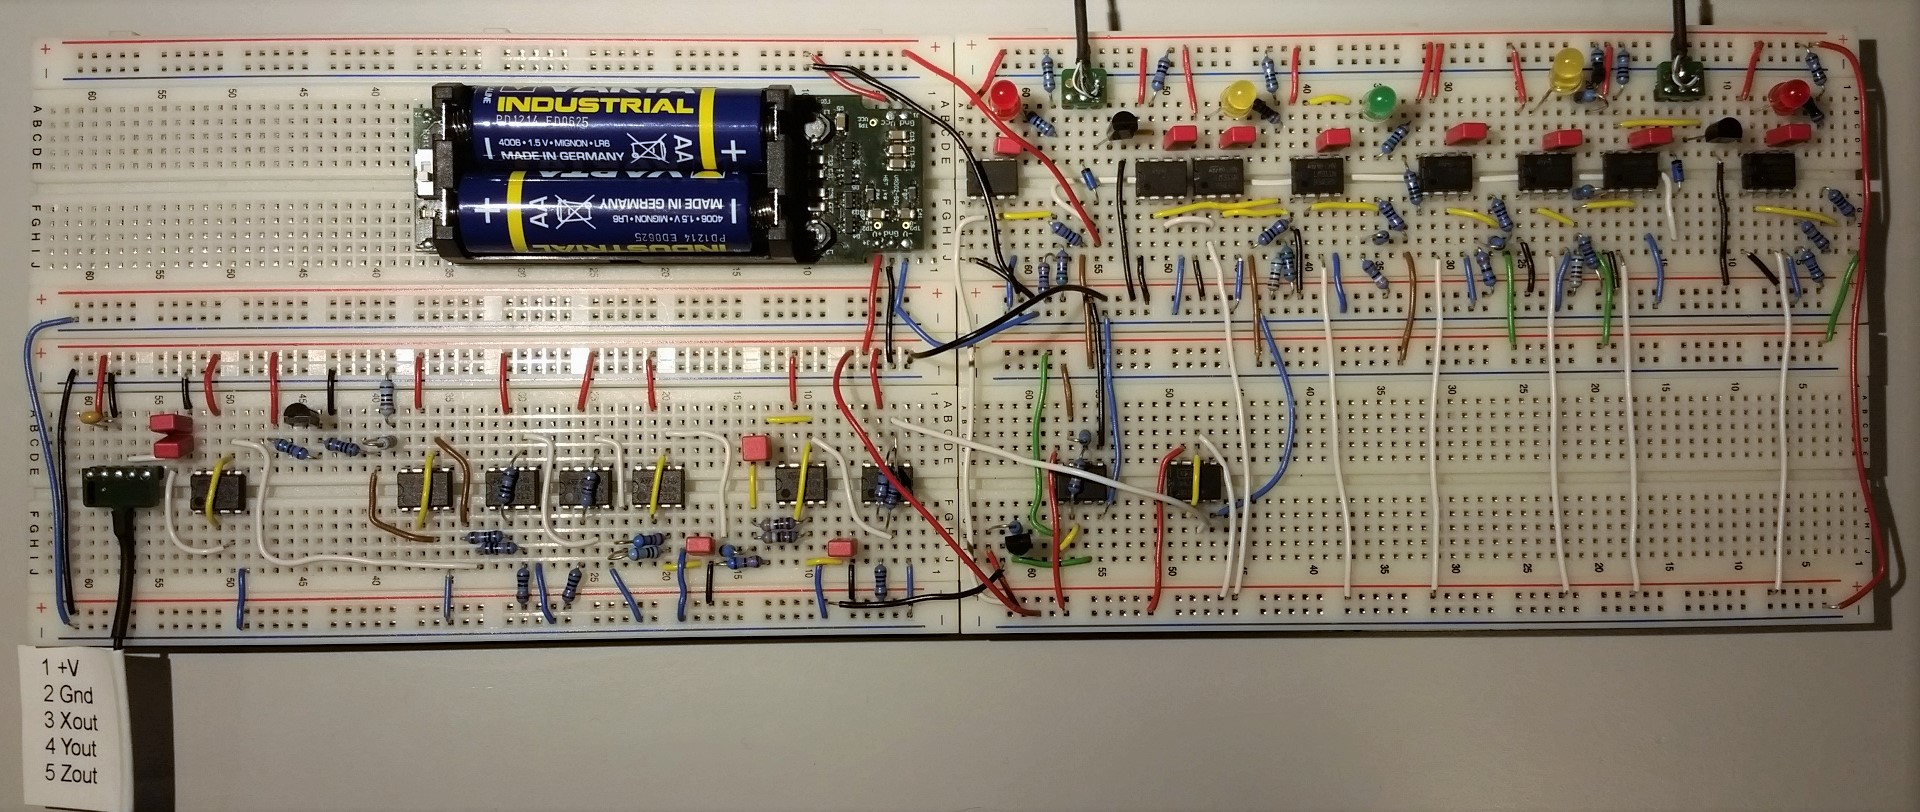
\includegraphics[scale=.22]{figures/cProblemloesning/Samlet_system2.jpg}
	\caption{På figuren ses implementeringen af systemet på to breadboards. Ledningernes farve symboliserer forskellige ting: De hvide leder signalet fra accelerometret igennem systemet og de røde og blå symboliserer hhv. den positive og negative strømforsyningen til de forskellige komponenter i systemet. De sorte ledninger leder til ground, og de gule ledninger fungerer som forbindelsesveje. De grønne og brune ledninger leder hhv. en positiv og negativ referencespænding til offsettet og komparatorerne.}
	\label{fig:samlet_system_real}
\end{figure}
\noindent Herefter er det samlede system klar til at blive testet. Det samlede system vil blive testet på to forskellige måder - først en test efter samme principper som i testen af accelerometeret og efterfølgende en test, hvor accelerometeret er placeret på en person jævnfør afsnit \ref{formaal_anvendelse} på side \pageref{formaal_anvendelse}. De to overordnede tests inddeles yderligere i to, da der for hver test kontrolleres, om den analoge samt digitale del fungerer efter hensigten.

\subsubsection{Test 1}
I den første test af det samlede system tages udgangspunkt i principperne fra testen af accelerometeret beskrevet i afsnit \ref{Acc_afsnit} på side \pageref{Acc_afsnit}. Det måles således, hvorvidt systemet opfylder de overordnede funktionelle krav jævnfør afsnit \ref{FunkKrav} på side \pageref{FunkKrav}, ved at placere accelerometeret i de definerede hældningsgrader, og herudfra vurdere om den korrekte feedback udløses.\\ 

\noindent\textbf{Test 1.a - analog}\\  
Ved den første test af den analoge del af systemet måles spændingsfaldet over LED'erne og vibratorerne før og efter aktivering. Derudover måles outputtet fra accelerometret lige ved aktivering af de forskellige komponenter. Disse målinger foretages med et multimeter. Resultatet fremgår af \tableref{Tab:resultat:test1a}:
\begin{table}[H]
	\centering
	\begin{tabular}{l|l|l|l|}
		\cline{2-4}
		\textit{}                                                                                 & \textit{\begin{tabular}[c]{@{}l@{}}Spændingsfald over \\ komponent før\\ udløst feedback\end{tabular}} & \textit{\begin{tabular}[c]{@{}l@{}}Output fra\\ accelerometer\\ ved udløst feedback\end{tabular}} & \textit{\begin{tabular}[c]{@{}l@{}}Spændingsfald over\\ komponent efter \\ udløst feedback\end{tabular}} \\ \hline
		\multicolumn{1}{|l|}{\textit{\begin{tabular}[c]{@{}l@{}}Rød LED\\ negativ\end{tabular}}}  & $1.3296$V                                                                                         & $1.5822$V                                                                                    & $2.0324$V                                                                                           \\ \hline
		\multicolumn{1}{|l|}{\textit{\begin{tabular}[c]{@{}l@{}}Vibrator\\ negativ\end{tabular}}} & $0.6$mV                                                                                           & $1.6005$V                                                                                    & $2.9995$V                                                                                           \\ \hline
		\multicolumn{1}{|l|}{\textit{\begin{tabular}[c]{@{}l@{}}Gul LED\\ negativ\end{tabular}}}  & $1.4310$V                                                                                         & $1.6005$V                                                                                    & $2.0700$V                                                                                           \\ \hline
		\multicolumn{1}{|l|}{\multirow{2}{*}{\textit{Grøn LED}}}                                  & \multirow{2}{*}{$1.4611$V}                                                                        & $1.6243$V                                                                                    & \multirow{2}{*}{$2.0196$V}                                                                          \\ \cline{3-3}
		\multicolumn{1}{|l|}{}                                                                    &                                                                                                   & $1.6377$V                                                                                    &                                                                                                     \\ \hline
		\multicolumn{1}{|l|}{\textit{\begin{tabular}[c]{@{}l@{}}Gul LED\\ positiv\end{tabular}}}  & $1.4247$V                                                                                         & $1.6562$V                                                                                    & $2.1187$V                                                                                           \\ \hline
		\multicolumn{1}{|l|}{\textit{\begin{tabular}[c]{@{}l@{}}Vibrator\\ positiv\end{tabular}}} & $0.1$mV                                                                                           & $1.6562$V                                                                                    & $3.1029$V                                                                                           \\ \hline
		\multicolumn{1}{|l|}{\textit{\begin{tabular}[c]{@{}l@{}}Rød LED\\ negativ\end{tabular}}}  & $1.3311$V                                                                                         & $1.6740$V                                                                                    & $2.0605$V                                                                                           \\ \hline
	\end{tabular}
	\caption{I tabellen ses resultatet fra målingerne af systemet.}
	\label{Tab:resultat:test1a}
\end{table}
\noindent Der ses i \tableref{Tab:resultat:test1a}, at der forekommer et spændingsfald over LED'erne, selvom de ikke afgiver synligt lys. Dette skyldes, at der løber en lækstrøm igennem dem, men denne er ikke tilstrækkelig for aktivering af synligt lys. På \figref{fig:samlet_system_LED} ses graferne for forholdet imellem spændingsfaldet over LED'erne og strømmen, der løber igennem, for de enkelte dioder. \cite{kingbright}
\begin{figure}[H]
	\centering
	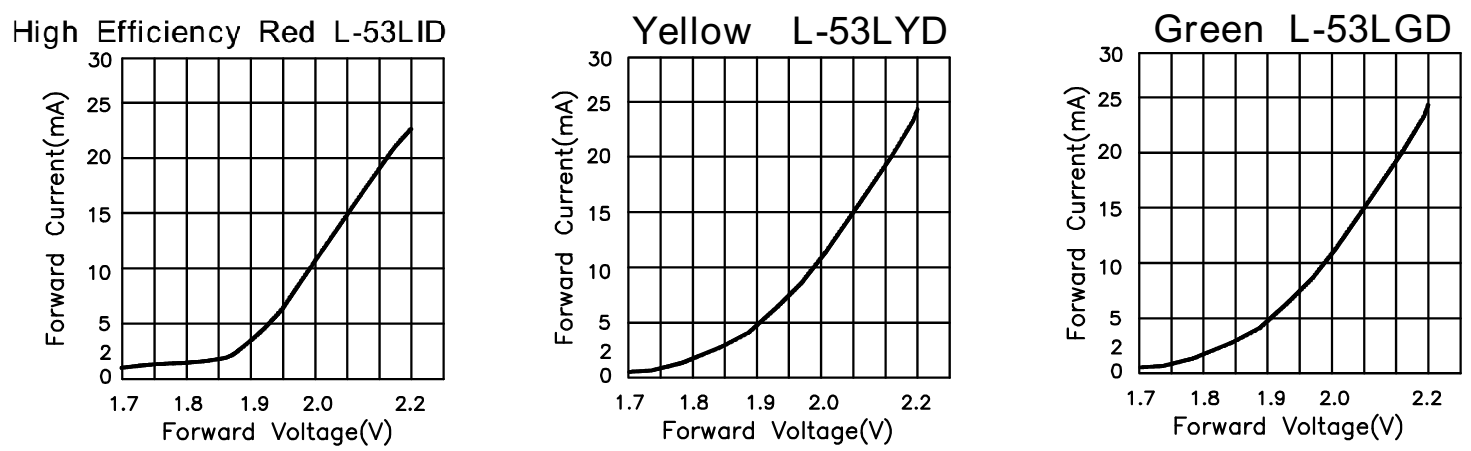
\includegraphics[scale=.45]{figures/cProblemloesning/Samlet_system_LED.PNG}
	\caption{På figuren ses der tre grafer for hhv. den røde, gule og grønne LED. Graferne viser forholdet imellem spændingsfaldet over LED'erne og strømmen, der løber igennem, for de enkelte dioder. \textit{(Revideret)} \cite{kingbright}}
	\label{fig:samlet_system_LED}
\end{figure}
\noindent Ifølge databladet for LED'erne vil de aktiveres ved $0.8$mA. Da der ikke er et lineært forhold imellem spændingsfaldet og strømmen på \figref{fig:samlet_system_LED}, er det ikke muligt at vurdere, om LED'erne faktisk er aktiverede ved målingerne i anden kolonne i \tableref{Tab:resultat:test1a}. Jævnfør afsnit \ref{Afs_Komparator} på side \pageref{Afs_Komparator} skal en LED modtage $20$mA for at afgive tydeligt lys. Da komparatorkonfigurationen er tilpasset til, at denne strøm skal løbe over LED'erne, kan det forventede spændingsfald aflæses på grafernes x-akse for de enkelte LED'er. Ud fra disse værdier beregnes afvigelsen for de målte spændingsfald. \\
I \tableref{Tab:resultat:test1a}'s fjerde kolonne ses det målte spændingsfald, når der teoretisk løber $20$mA over LED'en. De beregnede afvigelse ses i \tableref{tab:samlet_procent1a}. De teoretiske værdier for spændingsfaldet er aflæst på x aksen ud fra $20$mA på y aksen på \figref{fig:samlet_system_LED}.
\begin{table}[H]
	\centering
	\begin{tabular}{l|l|l|l|}
		\cline{2-4}
		\textit{} & \textit{\begin{tabular}[c]{@{}l@{}}Teoretisk\\ spændingsfald\end{tabular}} & \textit{\begin{tabular}[c]{@{}l@{}}Målte\\ spændingsfald\end{tabular}} & \textit{\% afvigelse} \\ \hline
		\multicolumn{1}{|l|}{\textit{\begin{tabular}[c]{@{}l@{}}Rød LED\\ negativ\end{tabular}}} & $2.14$V                                                                    & $2.0324$V                                                              & $5.03\%$              \\ \hline
		\multicolumn{1}{|l|}{\textit{\begin{tabular}[c]{@{}l@{}}Gul LED\\ negativ\end{tabular}}} & $2.15$V                                                                    & $2.0700$V                                                              & $3.73\%$              \\ \hline
		\multicolumn{1}{|l|}{\textit{Grøn LED}}                                                  & $2.14$V                                                                    & $2.0196$V                                                              & $5.63\%$              \\ \hline
		\multicolumn{1}{|l|}{\textit{\begin{tabular}[c]{@{}l@{}}Gul LED\\ positiv\end{tabular}}} & $2.15$V                                                                    & $2.1187$V                                                              & $1.46\%$              \\ \hline
		\multicolumn{1}{|l|}{\textit{\begin{tabular}[c]{@{}l@{}}Rød LED\\ negativ\end{tabular}}} & $2.14$V                                                                    & $2.0605$V                                                              & $3.71\%$              \\ \hline
	\end{tabular}
	\caption{I tabellen ses procentafvigelsen fra det forventede spændingsfald ved aktivering af LED'erne.}
	\label{tab:samlet_procent1a}
\end{table}
Det fremgår af \tableref{tab:samlet_procent1a}, at der forekommer afvigelser imellem det målte og det forventede spændingsfald for alle LED'erne. Alle de målte værdier ligger under de forventede værdier, hvorfor det må forventes, at LED'ernes lys er svagere end forventet. Da det typiske interval for spændingsfaldet ved synligt lys ligger på $1.7$-$1.9$V og maksimalt på $2.0$-$2.2$V jævnfør afsnit \ref{Afs_Komparator} på side \pageref{Afs_Komparator}, vurderes det imidlertid, at LED'erne udløser deres feedback efter hensigten.\\
De benyttede vibratorer aktiverer, når der sker et spændingsfald over dem på $2.3$V. \cite{Machinery2009} Teoretisk bør der ikke forekømme spændingsfald over vibratorerne, når disse er slukkede. Ud fra målingerne i \tableref{Tab:resultat:test1a} vurderes det, at dette er gældende. Ved udløst feedback sker der et spændingsfald for begge vibratorer på ca. $3$V. Dermed er spændingsfaldet over grænsen for aktivering, og det vurderes derfor, at vibratorerne udløser deres feedback efter hensigten. \\
Ud fra de målte outputværdier fra accelerometeret kan det beregnes, om feedbackmekanismerne aktiveres ved de definerede hældningsgrader jævnfør afsnit \ref{KomparatorAfs} på side \pageref{KomparatorAfs}. Dette gøres ved at tage outputværdien, trække offsettet i accelerometret fra og derefter dividere dette med hhv. -$0.0036$V og $0.0037$V for output i negativ og positiv retning.
\begin{align}\label{eq:graderLED_1}
\dfrac{(1.5822 - 1.6325)}{-0.0036} = 13.97^{\circ}\text{ for aktivering af rød LED i negativ retning} \\
\dfrac{(1.6005 - 1.6325)}{-0.0036} = 8.89^{\circ}\text{ for aktivering af gul LED samt vibrator i negativ retning} \\
\dfrac{(1.6243 - 1.6325)}{-0.0036} = 2.28^{\circ}\text{ for deaktivering af grøn LED i negativ retning} \\
\dfrac{(1.6377 - 1.6325)}{0.0037} = 1.41^{\circ}\text{ for deaktivering af grøn LED i positiv retning} \\
\dfrac{(1.6562 - 1.6325)}{0.0037} = 6.41^{\circ}\text{ for aktivering af gul LED samt vibrator i positiv retning} \\ \label{eq:graderLED_2}
\dfrac{(1.6740 - 1.6325)}{0.0037} = 11.22^{\circ}\text{ for aktivering af rød LED i positiv retning}
\end{align}
\noindent Der ses i overstående ligninger, at der er en afvigelse i accelerometerets hældning ift. de definerede grader for aktivering af feedbacken. Grunden til dette kan være, at referencespændingen til offsettet måles til $1.6302$V, hvilket er -$0.0023$V fra det teoretiske offset i accelerometret. Derved forskydes offsettet, og graderne for hældning af accelerometret i negativ retning vil blive større, mens graderne vil blive mindre i positiv retning. Derudover skal der tages højde for afvigelserne for de enkelte blokke i systemet, som undervejs er blevet accepteret. Disse vil tilsammen kunne skabe en større afvigelse for det samlede system. \\
På baggrund af målingerne og de vurderede fejlkilder godkendes systemet og det vurderes, at det virker efter hensigten.\\

\noindent\textbf{Test 1.b -  digital}\\ 

\subsubsection{Test 2}
I den anden test af det samlede system placeres accelerometeret på en forsøgsperson, der skal afprøve træningsforløbet med systemet. Formålet med denne test er at kontrollere, om den korrekte feedback udløses samt at vurdere, hvorvidt de definerede hældningsgrader er passende under træning med systemet. \\ 
\textbf{Test 2.a - analog}\\  
\textbf{Test 2.b - digital}\\ 
%%%%%%%%%%%%%%%%%% Nu skal lortet afsluttes
% !TeX spellcheck = da_DK
\chapter{Syntese}
\section{Diskussion}
Formålet med projektet er at udvikle et system, der kan give visuel og somatosensorisk biofeedback samt et digitalt output under apopleksipatienters balancetræning jævnfør afsnit \ref{formaal_anvendelse}, side \pageref{formaal_anvendelse}. Systemet er udviklet på baggrund af fastsatte hældningsgrader for risikozoner jævnfør afsnit \ref{ref:blokdiagram}, side \pageref{ref:blokdiagram}. På baggrund af design, simulering, implementering og test af systemets enkelte kredsløb ses det, at kravspecifikationerne overholdes. Der er imidlertid nogle områder indenfor de enkelte blokke, hvor det kan overvejes, hvorvidt andre målemetoder og designs kan anvendes.

\subsection{Målemetoder og pilotforsøg}
Der er flere steder i processen, hvor de endelige resultater kan være  påvirket. Systemet og de enkelte blokke er primært designet på baggrund af det udførte pilotforsøg i bilag \ref{Bilag:Pilotforsoeg}, side \pageref{Bilag:Pilotforsoeg}. De målte data under pilotforsøget kan være påvirket af forskellige faktorer, herunder lokalets temperatur på dagen for forsøgets udførelse samt støj fra omgivelserne. Dette kan have indflydelse på de beregnede værdier i systemets forskellige blokke.
Ydermere kan pilotforsøgets metode have væsentlig betydning ift. afvigelser i de beregnede værdier. Eksempelvis er spændingen ved de enkelte hældningsgrader udregnet ved at måle spændingen ved $0^{\circ}$ samt $\pm90^{\circ}$ og efterfølgende udregne spændingen for de enkelte hældningsgrader, hvor feedbacken skal udløses. Desuden er selve rotationsmålingerne udført ved, at en person har roteret accelerometeret med hånden til hhv. højre og venstre. Disse fejlkilder kunne have været begrænset ved anvendelse af mere præcist udstyr til opmåling af vinkler, hvor det desuden kunne være muligt at måle den præcise hældning ved de udvalgte grader frem for at udregne den.  \\
De målte data kan desuden være påvirket af afvigelser i de anvendte måleapparater, herunder multimeter og oscilloskop. De forskellige apparater kan kun måle et begrænset antal decimaler, og værdierne kan således variere ift. teorien. Derudover vil der være afvigelse ift. de anvendte komponenter under implementeringen, da der arbejdes med reelle komponenter. Visse komponenter, herunder operationsforstærkere og komparatorer, har i forvejen oplyst en afvigelse i deres datablade. Operationsforstærkeren af typen TL$081$ har f.eks. en inputoffsetspænding på typisk $5$mV \cite{Corporation1995}.

Testen af feedbackblokken er foretaget ved brug af oscilloskop. De målte tærskelværdier er sammenlignet med den værdi, hvor LED'en og vibratoren tænder, hvilket kan ses ved et spændingsfald. Oscilloskopet har indbygget en otte bit ADC til at afbillede målingerne digitalt. Denne konvertering gør, at oscilloskopet har en gråzone mellem målepunkterne, på ca. $0.04$V. I denne gråzone vil oscilloskopet ikke kunne vise den præcise værdi. Flere af tærskelværdierne samt spændingsfaldene for LED'erne og vibratorerne ligger i denne gråzone, er det vanskeligt at måle den nøjagtige forskel på værdierne. Derved er testen af komparatoren foretaget ved at tilnærme tærskelværdierne samt værdien for spændingsfaldet til det nærmeste målepunkt. Metoden er problematisk ved tærskelværdier med en lavere værdi, da $0.04$V udgør en større del af tærskelværdien, hvilket ses i \tableref{Tab:test-taendsluk}, side \pageref{Tab:test-taendsluk}, hvor værdien -$2^{\circ}$ afviger med $15.72$\%. Ved denne måling er tærskelværdien -$0.2373$V, hvilket er placeret i gråzonen, som går fra $0.200$V til $0.240$V og det samme er spændingsfaldet. Her bliver spændingsfaldet tilnærmet målepunktet på $0.200$V og tærskelværdi bliver tilnærmet $0.240$V. Tilnærmningen sket på baggrund af en vurdering af, hvilket værdierne lå nærmest. Derudover ville en oprunding af spændingsfaldetværdien betyde at den var ens med tærskelværdien, hvilket vurderes ikke var rigtigt ved aflæsning på oscilloskopet. 

En målemetode, hvori problematikken med oscilloskopets gråzone ikke gør sig gældende, er at opsætte et spændingstræ af tre modstande, hvor den midterste modstand byttes ud med et potentiometer. For at have en fast spænding kan spændingsreferencen på $2.5$V bruges. De to spændingsdeleres tærskelværdier kan udarbejdes således, at de danner et arbejdsområde, hvor det manuelt kan ændres vha. potentiometeret. Et multimeter kan tilkobles for at aflæse den reelle værdi i arbejdsområdet mere nøjagtigt. F.eks. kunne arbejdsområdet være mellem $0.200$V og $0.300$V, og da potentiometeret kan drejes $10$ omgange, vil der pr. omgang kunne justeres med $0.010$V, hvorfor gråzonen vil blive mindre end ved brugen af oscilloskopet. Metodens nøjagtighed afhænger af anvendte modstande i spændingstræet, spændingsreferencen, potentiometeret og multimetret. 

\subsection{Systemets design}
Der er blevet udarbejdet et system, som detekterer en kropshældning til hhv. højre eller venstre, men hvorvidt designet af de enkelte blokke i systemet er den optimale løsning kan diskuteres. I opsamlingsblokken justeres offsettet fra accelerometret ved $0$ g-påvirkning til $0$V, jævnfør afsnit \ref{Offset_Teori_Design}, side \pageref{Offset_Teori_Design}.Problemet med offsetjusteringen er, at accelerometerets offsetværdi kan ændre sig hver gang det benyttes. I systemet er et offset blevet fastsat til en bestemt værdi på baggrund af pilotforsøget og hvis accelerometerets offsetværdi afviger, fra den allerede fastsatte værdi, hver gang det benyttes vil dette påvirke tærskelværdierne. Problemet kan afvikles ved at benytte et højpasfilter, der designes til at dæmpe $0$Hz frekvens, hvorved offsettet dæmpes. Problemet ved denne løsning er, at det ikke er muligt at designe et ideelt højpasfilter, derved kan det ønskede signal også blive dæmpet. Samtidigt vil der opstå et problem, hvis patienten ikke er i bevægelse f.eks. ved en kropshældning på $8^{\circ}$, vil dette blive dæmpet, hvilket ikke ønskes. 

Offsetkredsløbet forsynes af en referencespænding, da kredsløbet er afhængig af en konstant spænding ift. at få en korrekt offsetjustering.  Hvis offsettet ikke justeres korrekt har dette indflydelse for systemets detektion af kropshældning, da accelerometeret er centreret omkring den forkerte værdi. Ved benyttelse af en referencespænding tilføjes ekstra komponenter til det samlede system, hvilket giver risiko for afvigelser, men det vurderes at være den mest optimale løsning, da et batteri ikke kan levere en konstant spænding over tid. Der forekommer altså et gradvist fald i den spænding, som batterierne kan yde, hvormed der på et tidspunkt ikke bliver leveret en tilstrækkelig spænding til offsettet. Der er stadig en uløst problematik ift. referencespændigen, da det er batterier, der fungerer som spændingsforsyning, jævnfør afsnit \ref{subsec:Spaendingsref}, side \pageref{subsec:Spaendingsref}, hvorfor en funktion, der oplyser brugeren, når referencenspændingen ikke længere fungerer efter hensigten, skal tilføjes. Problematikken kan løses ved at tilkoble referencespændingen til elnettet, hvorfor der forsynes med en konstant spænding. Hvis referencespændingen falder tilstrækkeligt, vil det have en påvirkning på hele systemet. Denne problemstilling gør sig også gældende for referencespændingen til feedbackblokken, hvorfor samme løsning til denne blok skal udføres. For feedbackblokken vil problematikken medføre en afvigelse i tærskelværdierne og dermed vil systemet ikke udløse feedback ved de korrekte hældningsgrader. 

Derudover designes offsetjusteringen og forstærkningen i opsamlingsblokken således, at det er to forskellige kredsløb, hvilket ikke er hensigtmæssigt, da det tilføjer flere komponenter til systemet med afvigelser. Hvis disse to kredsløb samles i ét kredsløb, vil dette forsimple blokken og dermed begrænse afvigelser. Denne løsning kunne også vælges at implementere ved filteret, hvor forstærkeren i tilpasningsblokken kunne designes som en del af filteret. Løsningen er imidlertid ikke valgt, da der i dette projekt ønskes en tydelig afgrænsning imellem de enkelte kredsløb for at gøre systemet mere overskueligt, hvorved identificering af eventuelle fejl muligvis er nemmere.\\

For at øge systemets præcision ift. at detektere patienternes kropshældning kan arbejdsområdet korrigeres. I tilpasningsblokken bliver signalet i systemet tilpasset til være $\pm3$V ved $\pm25^{\circ}$. Jævnfør afsnit \ref{Forstaerker_faktor3_afs}, side \pageref{Forstaerker_faktor3_afs} vurderes det, at en hældning over denne værdi ikke vil være relevant ift. at vurdere, hvorvidt patienten er faldet. Dette bør undersøges nærmere for at underbygge denne vurdering yderligere. En evt. variation fra denne fastsatte hældningsværdi vil betyde, at forstærkningsfaktoren skal ændres. Dette vil medføre, at det efterfølgende arbejdsområde vil blive enten større eller mindre, hvorfor tærskelværdierne i feedbackblokken også skal ændres.\fxnote{NTK: Løsning: variabel forstærker = potentiometer} Hvis der er evidens for at øge arbejdsområdet kan tærskelværdierne indstilles med større præcision, da en grads forskel i hældning derved vil give en større spændingforskel. Hvorvidt dette vil mindske afvigelsen mellem den forventede og målte hældninggrad, jævnfør afsnit \ref{samlet_systemtest_ref}, side \pageref{samlet_systemtest_ref} skal undersøges. 

\subsection{Brugervenlighed}
Det kan være kompliceret at give feedback til patienter med følger af apopleksi, da de kan have kognitive problemer jævnfør afsnit \ref{Krav_biofeedback}, side \pageref{Krav_biofeedback}. Det skal derfor vurderes, hvorvidt flere typer feedback ad gangen er hensigtsmæssigt for patienterne, samt hvordan feedbacken anvendes.  

Der bør ift. den somatosensoriske feedback vurderes hvilken side, der er mest hensigtsmæssig at udløse feedbacken i; Det kan i praksis undersøges, om det virker bedst for patienterne, at vibrationen udløses i samme side som hældningen sker til eller, om det fungerer bedre, at vibrationen sker i modsatte side. Hvis den sidste mulighed er mest optimal, vil løsningen være at sætte vibratorene omvendt på patienten. Det kan desuden overvejes, om der kan implementeres en tredje feedbackform, auditiv feedback, hvor patienten advares vha. lyde, der angiver hældningsgraden. Denne feedbackform kan umiddelbart være vanskelig at anvende, da apopleksipatienter, jævnfør afsnit \ref{Krav_biofeedback}, side \pageref{Krav_biofeedback}, ofte er ældre og derved kan have nedsat hørelse \cite{Sundhedsstyrelsen2011}. Derudover kan betydningen af lydene være svær at huske, da det ikke er et system, der i forvejen er indlært som ved den visuelle feedback. For at øge effekten af feedbacken kan systemet udvikles til at fravælge og tilvælge flere former for feedback, alt efter hvilken patienten responderer bedst på.

Softwaren er designet til at gemme en billedfil, men det kan diskuteres, hvorvidt det er mere hensigtsmæssigt at gemme samtlige datapunkters værdi. Fordelen ved at gemme alle patienternes datapunkter er, at det fagkyndige personale kan udføre yderligere beregninger for patientens øvelse, herunder gennemsnitshældning, antallet af udsving over tærskelværdier og det præcise maksimale udsving uden fald. Dette vil give mere information om patientens balancefunktion samt progression under rehabiliteringforløbet. \\
Det er problematisk, at systemet er designet således, at patienten skal bevæge sig under øvelsen for at starte og stoppe optagelsen, da der ville optages unødvendig bevægelser. En løsning på denne problematik er at forsinke optagelsen med $15$ sekunder efter aktivering i interfacet, hvorved patienten har tid til at tage udgangsposition for øvelsen. Ellers kan brugeren efter øvelsen redigere på x-aksen, hvis redigering igennem MATLAB muliggøres. Det kan også være en mulighed, at stop- og startfunktion for interfacet placeres omkring accelerometeret på patienten, hvorved vedkommende selv kan trykke, når udgangspositionen for den pågældende øvelse er taget.

\subsection{Samlet systemtest }
I simuleringen af det samlede system aktiveres det forventede antal LED'er og vibratorere ved de enkelte tærskelværdier. Systemet blev altså simuleret til at fungere efter hensigten, jævnfør (overordende funktionelle krav). Hvis afvigelsen mellem definerede og simulerede hældningsgrader undersøges, ses det, at feedbacken ikke udløses ved den korrekte hældningsgrad. Den største afvigelse ses for den røde LED i positiv retning, hvilket er problematisk, da denne LED lyser, når patienten er i fare. En afvigelse af denne størrelse er i højere grad acceptabel for den grønne LED, eftersom denne lyser, når patienten befinder sig indenfor risikozonerne. Det bør derfor undersøges og simuleres, hvorvidt en korrektion af offsettet og medkalkulering at operationsforstærkernes indbyggede offset vil have en indflydelse på det samlede system og dens detektion af definerede hældningsgrader. 

Når det samlede system implementeres og testes kan diskuteres, hvorvidt aflæsningen af accelerometerets output er foretaget præcist, da outputtet aflæses ved forsøgsafviklernes vurdering af tidspunktet for udløst feedback. En mere præcis metode til dette vil eventuelt være at benytte et potentiometer, da der i test $1$ roteres manuelt, hvorfor spændingen fra accelerometret ikke er konstant. Dette kan under test erstatte accelerometret, hvorved det præcise output, der sendes ind i resten af systemet, kan aflæses med et multimeter.\fxnote{NTK: potentiometret sættes op i en spændingstre med to spændingsdelere på hver side, som angiver "arbejdsområdet". Der kan drejes 10 omgange på potentiometret, hvorved den kan fungere som en variabel forstærker inden for arbejdsområdet.} Derudover vil tidspunktet for udløst feedback være mere præcist, da spændingen fra potentiometeret kan holdes konstant og måles mere nøjagtigt. Ved anvendelse af potentiometeret vil der imidlertid være flere tolerancer, som skal tages højde for, da designet er mere omfattende. Ifølge målte hældningsgrader under implementeringen ses endnu en afvigelse ift. bestemte hældningsgrader. Jævnfør afsnit \ref{samlet_systemtest_ref}, \pageref{samlet_systemtest_ref} måles accelerometerets offset til $1.6302$V i den samlede systemtets, hvilket afviger fra offsettet i pilotforsøget, jævnfør bilag \ref{Bilag:Pilotforsoeg}, \pageref{Bilag:Pilotforsoeg}. Eftersom tærskelværdierne er beregnet ud fra offsettet i pilotforsøget kan disse påvirkes, hvis offsettet i accelerometeret ikke er denne værdi og kan bl.a. forklare afvigelsen på hældningsgraderne. Men eftersom afvigelsen også ses ved simuleringen gør en anden faktor sig også gældende, såsom afvigelsen på de enkelte komponenter. 
I testen blev det derudover undersøgt hvilken effekt referencespændingen har på offsetjusteringen og dermed hældningsgraderne. Det ses, at hvis der tages højde for kalibrering af offsetjustering er det muligt at gøre afvigelsen mellem de forventede og målte hældningsgrader generelt lavere. 

Det kan diskuteres på baggrund af den samlede systemtest af den digitale del af systemet, om programmet er brugervenligt og optimalt for det fagkyndige personale. For optimering af brugervenligheden kan der eventuelt tilføjes funktioner, som kan gøre det muligt for personalet at indtaste og hente informationer om patienten igennem programmet, herunder eksempelvis navn, CPR og dato. Derudover kan området for y-aksen evt. afgrænses, således den evt. går fra $\pm25^{\circ}$, hvorved det vil blive lettere at aflæse målingerne præcist, da det forventes, at patienten vil holde sig inden for dette afgrænset område. \\
\clearpage


%\chapter{Syntese}
%\section{Diskussion}
%Formålet med projektet er at udvikle et system, der kan give visuel og somatosensorisk biofeedback samt et digitalt output under apopleksipatienters balancetræning jævnfør afsnit \ref{formaal_anvendelse}, side \pageref{formaal_anvendelse}. Systemet er udviklet på baggrund af fastsatte hældningsgrader for risikozoner jævnfør afsnit \ref{ref:blokdiagram} på side \pageref{ref:blokdiagram}.

%\subsection{Målemetoder og pilotforsøg}
%Der er flere steder i processen, hvor de endelige resultater kan være blevet påvirket. Systemet og de enkelte blokke er primært designet på baggrund af det udførte pilotforsøg i bilag \ref{Bilag:Pilotforsoeg}, side \pageref{Bilag:Pilotforsoeg}. De målte data under pilotforsøget kan være påvirket af forskellige faktorer, herunder lokalets temperatur på dagen for forsøgets udførelse samt støj fra omgivelserne. Dette kan have indflydelse på de beregnede værdier i systemets forskellige blokke.
%Ydermere kan pilotforsøgets metode have væsentlig betydning ift. afvigelser i de beregnede værdier. Eksempelvis er spændingen ved de enkelte hældningsgrader udregnet ved at måle spændingen ved $0^{\circ}$ samt $\pm90^{\circ}$ og efterfølgende udregne spændingen for de enkelte grader, hvor feedbacken skal udløses. Desuden er selve rotationsmålingerne udført ved, at en person har roteret accelerometeret med hånden til hhv. højre og venstre. Disse fejlkilder kunne have været begrænset ved anvendelse af mere præcist udstyr til opmåling af vinkler, hvor det desuden kunne være muligt at måle den præcise hældning ved de udvalgte grader frem for at udregne den.  \\
%De målte data kan desuden være påvirket af afvigelser i de anvendte måleapparater, herunder multimeter og oscilloskop. De forskellige apparater kan kun måle et begrænset antal decimaler, og værdierne kan således variere ift. teorien. Derudover vil der være afvigelse ift. de anvendte komponenter under implementeringen, da der arbejdes med reelle komponenter. Visse komponenter, herunder operationsforstærkere og komparatorer, har i forvejen oplyst en afvigelse i deres datablade. Operationsforstærkeren af typen TL$081$ har f.eks. en inputoffsetspænding på typisk $5$mV \cite{Corporation1995}. %Andre komponenter er blevet målt, herunder modstande og kondensatorer, og en eventuel afvigelse er medkalkuleret i systemet for at minimere afvigelserne, så vidt det var muligt. 

%\subsection{Problemløsning}
%Ved design, simulering, implementering og test af systemets enkelte kredsløb ses det, at alle overholder de fastsatte krav og tolerancer. Der er imidlertid nogle områder indenfor de enkelte blokke, hvor det kan overvejes, hvorvidt andre målemetoder og designs kan anvendes.

%\subsubsection{Referencespænding til offset}
%Implementeringen af en referencespænding til forsyning af offsetkredsløbet tilføjer ekstra komponenter til det samlede system, hvilket giver større risiko for afvigelser. Dette vurderes imidlertid at være den mest optimale løsning sammenlignet med at anvende eksempelvis et batteri, da dette ikke kan afgive en konstant spænding over tid. Der er en uløst problematik ift. referencespændingen, da det er batterier, der fungerer som spændingsforsyning, jævnfør afsnit \ref{subsec:Spaendingsref} på side \pageref{subsec:Spaendingsref}. Dermed forekommer et gradvist fald i den spænding, som batterierne kan yde over tid, hvormed der med tiden heller ikke kan leveres en tilstrækkelig spænding fra referencen. Dette kan have konsekvenser ift. at få justeret offsettet korrekt. Det kan derfor være hensigtsmæssigt at tilføje en funktion, der oplyser brugeren, når referencen ikke længere kan udsende den forventede spænding. Problematikken kan løses ved at tilkoble referencespændingen til elnettet, hvorfor der forsynes med en konstant spænding. Hvis referencespændingen falder tilstrækkeligt, vil det have en påvirkning på hele systemet. %Denne funktion kunne eventuelt være aktivering af en LED eller en auditiv alarm.

%\subsubsection{Opsamling}
%I opsamlingblokken bliver offsettet fra accelerometret ved $0$g påvirkning justeret til $0$V jævnfør afsnit \ref{Offset_Teori_Design} på side \pageref{Offset_Teori_Design}. Da formålet med blokken i denne sammenhæng er at fjerne offsettet helt, kan det være en mulighed at anvende et højpasfilter, som dæmper frekvenserne fra offsettet.\fxnote{NTK: Når accelerometeret detekterer offsetværdien er påvirkningen $0$g, hvilket udgør de laveste frekvenser i signalet. Disse kan identificeres og dermed dæmpes med et højpasfilter, således at offsettets frekvenser er dæmpede på det samlede signal.} Ved denne løsning skal det medregnes, at frekvenserne ikke fjernes helt, og det kræver derfor, at de er dæmpet tilstrækkeligt til, at de ikke har indflydelse på det samlede signal. \\
%Det kan desuden overvejes, om det vil være mere optimalt at sammenlægge offsetjusteringen og forstærkningen i opsamlingsblokken til ét kredsløb, hvilket kan forsimple blokken og dermed begrænse visse afvigelser, da der indgår færre komponenter. Denne løsning er imidlertid ikke valgt, da der i dette projekt ønskes en tydelig afgrænsning imellem de enkelte kredsløb for at gøre systemet mere overskueligt, hvorved identificering af eventuelle fejl muligvis er nemmere.\\
%Accelerometeret skal under træningen være placeret øverst på sternum. Det kan i denne forbindelse overvejes, om der ved målingerne forekommer støj fra kroppen; eksempelvis i form af påvirkning fra hjerte og lunger.\fxnote{opgave: skal diskutteres noget mere.} 

%\subsubsection{Filter}
%På baggrund af \eqref{eq:orden3}, side \pageref{eq:orden} bliver der bestemt, at der skal udarbejdes et 3. ordens lavpasfilter til at dæmpe uønskede frekvenser i det opsamlede signal. Kondensatorerne i kredsløbet bliver valgt ud fra, hvad der er til rådighed i laboratoriet, og modstandene i kredsløbet bliver efterfølgende udregnet ud fra disse. I praksis kan der anvendes en reel kondensator og indsætte dennes målte værdi i ligningen istedet for den teoretiske, hvorved der muligvis vil være behov for andre modstande. \\\fxnote{Der skal diskuttere fordele og ulemper ved butter, Tschebyschev- og Besselfiltre.}%ville det have været mere hensigtsmæssigt at afprøve flere forskellige kondensatorer og vælge dem, der gav den mindste afvigelse ift. sammensætning af modstandene. \\
%Jævnfør afsnit \ref{Filter_afsnit} på side \pageref{Filter_afsnit} blev der valgt at anvende et Butterworth filter frem for de andre former for filter for at opnå maksimal fladhed i pas- og stopbåndet. Hvorvidt dette er blevet opfyldt vides via teorien, at Butterworth filtret opnår den maksimale fladhed i pas- og stopbåndet ift. f.eks. Tschebyschev- og Besselfiltre. \cite{Carter2013} Der kunne dog være forsøgt at designe et 3. ordens Tschebyschev- og Besselfilter for at påvise denne fladhed i Butterworth filtret. Derved kunne der opnås endnu en parameter, der beskriver kvaliteten af det udarbejdede filter og et mere kvalificeret valg kunne blive truffet ift. hvilket filter, der er mest optimalt til dette system. \\  
%Ved simulering af filteret med de beregnede modstande er der opstået nogle afvigelser i pasbåndsfrekvensen, som ligger over de fastsatte tolerancer. Dette problem er imidlertid blevet løst, da de udregnede modstande under simuleringen er blevet erstattet med de teoretiske værdier for de reelle modstande, som skal indgå i implementeringen af kredsløbet. Årsagen til dette er ukendt, da simulering med de præcise udregnede værdier bør give de mindste afvigelser, men det er besluttet at acceptere blokken, da de reelle modstande også kan bruges i implementeringen uden yderligere afrunding.\fxnote{men så havde de reelle værdier jo også afvigelser fra de teoretiske. Havde det ikke være mere korrekt at bruge de reelle modstandes reelle værdier?}

%\subsubsection{Tilpasning}
%I tilpasningsblokken bliver signalet i systemet tilpasset til være $\pm3$V ved $\pm25^{\circ}$. Jævnfør afsnit \ref{Forstaerker_faktor3_afs}, side \pageref{Forstaerker_faktor3_afs} vurderes det, at en hældning over denne værdi ikke vil være relevant ift. at vurdere, hvorvidt patienten er faldet. Dette kan undersøges nærmere for at underbygge denne vurdering yderligere. En eventuel variation fra denne fastsatte hældningsværdi vil betyde, at forstærkningsfaktoren skal ændres. Dette vil medføre, at det efterfølgende arbejdsområde vil blive enten større eller mindre, hvorfor tærskelværdierne i feedbackblokken også skal ændres.\fxnote{NTK: Løsning: variabel forstærker = potensiometer} Ved et større arbejdsområde vil tærskelværdierne kunne indstilles mere præcist, da en grads forskel i hældning derved vil give en større spændingsforskel.

%\subsubsection{Spændingsreference til komparator}
%Spændingsreferencen til feedbackkonfigurationen er opbygget efter de samme principper som referencespændingen til offsettet. Der opstår samme problematik som for spændingsreferencen til offsettet; spændingsforsyningen til referencen er udgjort af batterier, hvorfor referenceværdien med tiden ikke kan opretholdes. For feedbackblokken vil dette det betyde en afvigelse i tærskelværdierne i de enkelte komparatorer, hvorfor der ikke længere vil udløses feedback ved de rigtige hældningsgrader. Det vil også her være essentielt med en indikation til brugeren om, at referencespændingen ikke længere ligger på den krævede værdi. 

%\subsubsection{Feedback}
%Det kan være kompliceret at give feedback til patienter med følger af apopleksi, da de kan have kognitive problemer jævnfør afsnit \ref{Krav_biofeedback}, side \pageref{Krav_biofeedback}. Det skal derfor vurderes, hvorvidt flere typer feedback ad gangen er hensigtsmæssigt for patienterne, samt hvordan feedbacken anvendes. %Det vurderes, at den visuelle feedback vil være essentiel for patienterne i begyndelsen af rehabiliteringsforløbet. 
%For at lære systemet og dets anvendelse at kende, er den visuelle feedback opbygget ud fra samme princip, som et lyskryds, hvilket er et kendt system for patienterne. Dette skyldes, at farverne tydeligt viser, hvilket område patienten befinder sig indenfor, samt hvilken retning hældningen sker i. Desuden er feedbacken sammensat ud fra samme princip som et lyskryds, hvilket er et kendt system for patienten. Dette hjælper til at lære systemet og dets anvendelse af kende% og stiller ikke store krav til patientens evne til at fokusere på feedbacken. Den somatosensoriske feedback vil være at foretrække for patienter, som er længere i rehabiliteringsprocessen og har forbedret balance. Denne feedbackform stiller større krav til patienten end den visuelle feedback, da hældningsintervallerne ikke er tydeligt afgrænset. Derudover er der ingen feedback vedrørende patientens udgangsposition, da der ikke er vibration ved den grønne LED, hvorved patienten skal have fornemmelse for stabil udgangsposition. Desuden er der én vibrationshastighed, hvilket gør, at patienten ikke får feedback om personen er i første eller anden risikozone. De to feedbackformer er adskilt fra hinanden i systemet, hvormed det i praksis vil være muligt at vurdere hvilken feedbacktype, der skal anvendes til den enkelte patient.

%Der bør ift. den somatosensoriske feedback vurderes hvilken side, der er mest hensigtsmæssig at udløse feedbacken i; Det kan i praksis undersøges, om det virker bedst for patienterne, at vibrationen udløses i samme side som hældningen sker til eller, om det fungerer bedre, at vibrationen sker i modsatte side. Hvis den sidste mulighed er mest optimal, vil løsningen være at sætte vibratorene omvendt på patienten. Det kan desuden overvejes, om der kan implementeres en tredje feedbackform, audiotiv feedback, hvor patienten advares vha. lyde, der angiver hældningsgraden. Denne feedbackform kan umiddelbart være vanskelig at anvende, da apopleksipatienter, jævnfør afsnit \ref{Krav_biofeedback}, side \pageref{Krav_biofeedback}, ofte er ældre og derved kan have nedsat hørelse \cite{Sundhedsstyrelsen2011}. Derudover kan betydningen af lydene være svær at huske, da det ikke er et system, der i forvejen er indlært som ved den visuelle feedback.

%Testen af feedbackkonfigurationen er foretaget ved brug af oscilloskop. De målte tærskelværdier er sammenlignet med den værdi, hvor LED'en og vibratoren tænder, hvilket kan ses ved et spændingsfald. Oscilloskopet har indbygget en otte bit ADC-konverter til at afbillede målingerne digitalt. Denne konvertering gør, at oscilloskopet har en gråzone mellem målepunkterne, der er på ca. $0.04$V. I denne gråzone vil oscilloskopet ikke kunne vise den præcise værdi. Da flere af tærskelværdierne samt spændingsfaldene for LED'erne og vibratorerne ligger i denne gråzone, er det vanskeligt at måle den nøjagtige forskel på værdierne. Derved er testen af komparatoren foretaget ved at tilnærme tærskelværdierne samt værdien for spændingsfaldet til det nærmeste målepunkt. Metoden er problematisk ved tærskelværdier med en lavere værdi, da $0.04$V udgør en større del af tærskelværdien, hvilket ses i \tableref{Tab:test-taendsluk}, side \pageref{Tab:test-taendsluk}, hvor værdien  -$2^{\circ}$ afviger med $15.72$\%. Ved denne måling er tærskelværdien -$0.2373$V, hvilket er placeret i gråzonen, som går fra $0.200$V til $0.240$V og det samme er spændingsfaldet. Her bliver spændingsfaldet tilnærmet målepunktet på $0.200$V, da det vurderes, at den ligger nærmest.\fxnote{opgave: skrive hvorfor den grønne LED må have en større afvigelse end den gule og røde LED}

%En målemetode, hvori problematikken med oscilloskopets gråzone ikke gør sig gældende, er at opsætte et spændingstræ. Dette fungerer som to spændingsdelere med et potentiometer, der erstatter den midterste modstand. For at have en fast spænding kan spændingsreferencen på $2.5$V bruges. De to spændingsdeleres tærskelværdier kan udarbejdes således, at de danner et arbejdsområde, hvor det manuelt kan ændres vha. potentiometeret. Et multimeter kan tilkobles for at aflæse den reelle værdi i arbejdsområdet mere nøjagtigt. F.eks. kunne arbejdsområdet være mellem $0.200$V og $0.300$V, og da potentiometeret kan drejes $10$ omgange, vil der pr. omgang kunne justeres med $0.010$V, hvorfor gråzonen vil blive mindre end ved brugen af oscilloskopet. Metoden nøjagtighed afhænger af anvendte modstande i spændingstræet, spændingsreferencen, potentiometeret og multimetret. %Gråzonen afhænger ved denne metode af, hvor præcis værdierne er i spændingstræet. Denne præcision afhænger af modstandene der benyttes. Desuden afhænger metoden af multimeteres nøjagtighed ift. den værdi der måles, og den værdi der vises på interfacet.   

%\subsubsection{ADC}
%I resultaterne fra testen af ADC'en konkluderes det, at en for lav samplingsfrekvens ift. signalet medfører et kantet signal. Dette gøres på baggrund af de grafer, som fremkommer ved målingerne jævnfør afsnit \ref{ADC_afsnit}, side \pageref{ADC_afsnit}. For at underbygge denne konklusion kan det være en mulighed at foretage en test for aliasing.%, hvor inputsignalets frekvens øges yderligere. 
%Hvis resultatet af denne måling skal stemme overens med den nuværende konklusion, skal grafen for den nye måling være mere kantet som et udtryk for, at der opsamles med for få datapunkter til, at der kan opnås et repræsentativt resultat.

%\subsubsection{USB-isolator}
%Da der ikke er udført en decideret test af USB-isolatoren og den opfylder de opstillede krav jævnfør afsnit \ref{USB_afsnit} på side \pageref{USB_afsnit} vurderes det, at der ikke er nogle væsentlige faktorer, der bør overvejes ift. denne blok.

%\subsubsection{Software}
%For at kunne anvende softwaren kræver det, at brugeren har en computer med programmet MATLAB. Derudover skal computeren have mulighed for at åbne målingsfilen, der er gemt som en billedefil. På denne måde kan patienten eller plejepersonalet videresende data til alle, som det kunne være relevant for. %Det er ikke muligt at manipulere med grafen, da det er en billedefil, hvilket stiller en række krav til, at softwaren beregner og viser de nødvendige oplysninger for f.eks. plejepersonalet. 
%Hvorvidt det skal være muligt for fagkyndige personale at kunne redigere grafen kan diskuteres. Som softwaren er nu skal plejepersonalet benytte fotoshop for redigering af grafen, da det er en billedfil. En anden mulighed kunne være, at filen blev gemt i MATLAB, hvilket gør, at plejepersonalet kan redigere og manipulere grafen efter, at filen er gemt. Der kunne f.eks. være behov for at redigere på akserne, hvorved der kan zoomes yderligere ind på et bestemt punkt på grafen. \\
%Softwaren er designet til at gemme en billedfil, men det kan diskuteres, om det vil være hensigtsmæssigt at gemme samtlige datapunkters værdi. Det fagkyndige personale kan muligvis bruge datapunkternes værdier til at udføre yderligere beregninger for patientens øvelse, herunder gennemsnitshældning, antallet af udsving over tærskelværdier og det præcise maksimale udsving uden fald. Dette vil give mere information om patientens progression. \\
%Det vil være optimalt for patienten at have en anden person til rådighed under øvelsen, som kan starte og stoppe optagelsen. Dette skal gøres i softwarens interface, hvilket gør, at øvelsen endnu ikke kan udføres selvstændigt. En løsning på denne problematik kan være, at optagelsen forsinkes med $15$ sekunder efter aktivering i interfacet, hvorved patienten har tid til at tage udgangsposition for øvelsen. Ellers kan brugeren efter øvelsen redigere på x-aksen, hvis redigering igennem MATLAB blev en mulighed. Det kan også være en mulighed, at stop- og startfunktion for interfacet placeres omkring accelerometeret på patienten, hvorved vedkommende selv kan trykke, når udgangspositionen for den pågældende øvelse er taget.

%\subsubsection{Spændingsforsyning}
%Jævnfør afsnit \ref{Spaendingsforsying}, side \pageref{Spaendingsforsying} anvendes spændingsforsyningen til at forsyne hhv. spændingsreferencerne samt de øvrige blokke i systemet. På baggrund af teori og tests fremgår det, at det er essentielt, at spændingsforsyningen leverer den forventede spænding, da det ellers vil påvirke hele systemets funktion. Det kan dermed også være en fordel at tilføje en funktion til systemet, der informerer brugeren, når spændingsforsyningen ligger under den forventede værdi. 
 
%\subsection{Det samlede system}
%Det kan diskuteres, hvorvidt aflæsningen af accelerometerets output under den samlede test er foretaget korrekt, da outputtet aflæses ved forsøgsafviklernes vurdering af tidspunktet for udløst feedback. En mere præcis metode til dette vil eventuelt være at benytte et potentiometer, da der i test $1$ roteres manuelt, hvorfor spændingen fra accelerometret ikke er konstant. Dette kan under test erstatte accelerometret, hvorved det præcise output, der sendes ind i resten af systemet, kan aflæses med et multimeter.\fxnote{NTK: potensiometret sættes op i en spændingstre med to spændingsdelere på hver side, som angiver "arbejdsområdet". Der kan drejes 10 omgange på potensiometret, hvorved den kan fungere som en variabel forstærker inden for arbejdsområdet.} Derudover vil tidspunktet for udløst feedback være mere præcist, da spændingen fra potentiometeret kan holdes konstant og måles mere nøjagtigt. Ved anvendelse af potentiometeret vil der imidlertid være flere tolerancer, som skal tages højde for, da designet er mere omfattende. \\
%Det kan diskuteres på baggrund af den samlede systemtest af den digitale del af systemet, om programmet er brugervenligt og optimalt for det fagkyndige personale. For optimering af brugervenligheden kan der eventuelt tilføjes funktioner, som kan gøre det muligt for personalet at indtaste og hente informationer om patienten igennem programmet, herunder eksempelvis navn, CPR og dato. Derudover kan spektret for y-aksen eventuelt afgrænses, således den evt. går fra $\pm25^{\circ}$, hvorved det vil blive lettere at aflæse målingerne præcist, da det forventes, at patienten vil holde sig inden for feedbackspektret. \\

% !TeX spellcheck = da_DK
\section{Konklusion}
I dette projekt er et biofeedbacksystem blevet udarbejdet. Dette kan opsample et biologisk signal fra et accelerometer, der informerer om en apopleksipatients kropshældning. Accelerometerets g-påvirkning ved den specifikke hældning konverteres til en elektrisk spænding, som bruges til at give en visuel og somatosensorisk feedback. Ud over den analoge del af systemet kan den digitale del af afbillede det biologiske signal, samt gemme patientdata vha. udviklet software. Apopleksipatienter kan med fordel anvende systemet til træning af balancen vha. forskellige balanceøvelser under rehabiliteringsprocessen, eftersom systemet giver information omkring kroppens position i det frontale plan. Systemet er designet således, at det måler patienternes kropshældning samt angiver, hvilken retning hældningen sker i vha. biofeedback. Ifølge studier, jævnfør \ref{MekBioFeed}, side \pageref{MekBioFeed} medfører en signifikant forbedring af balancefunktionen. Det vurderes derfor, at hvis patienterne anvender systemet i kombination med balanceøvelser under rehabiliteringsprocessen, vil dette kunne hjælpe dem til en forbedret balance. 

Et biofeedbacksystem med et accelerometer, der hjælper apopleksipatienters balancetræning under rehabilitering, kan designes ved, at systemet starter med en opsamlingsblok. Denne omfatter accelerometeret, offsetjustering og en forstærker. Herefter følger en filtreringsblok, der omfatter et lavpasfilter, inden systemet forgrenes i hhv. en analog og digital del. Næste blok i den analoge del af systemet er en tilpasningsblok, hvor signalet forstærkes og tilpasses et mindre range for hældningsgrader. Signalet ledes herefter over i feedbackblokken, der indeholder en komparatorkonfiguration tilkoblet de forskellige feedbackkomponenter, der aktiveres ved forskellige hældningsgrader og informerer patienten herom. Den visuelle feedback omfatter LED'er i en konfiguration designet efter princippet i et trafiklys, mens den somatosensoriske feedback omfatter vibration. 
I den digitale del af systemet bliver det analoge signal fra filtret sendt ind i en ADC-blok for at konvertere det til et digitalt signal. Herefter ledes signalet igennem en blok indeholdende en USB-isolator og til sidst ind i computeren, der opsamler og behandler signalet i MATLAB samt afbilleder som et realtime plot. Plottet kan herefter gemmes til senere brug og analyse af det fagkyndige personale.

Designet af systemets blokke er blevet evalueret igennem simuleringer og tests, hvor det er undersøgt, om blokkene overholder de opstillede kravspecifikationer og tolerancer. Alle blokkene er på baggrund af de udførte tests blevet godkendt til at indgå i det samlede system. Der bliver afslutningsvis foretaget en test af det samlede system, hvor resultatet viste, at de overordnede funktionelle krav for systemet er opfyldt. I denne test blev det vurderet, at der kunne tolereres større afvigelser end i de udførte tests af de enkelte blokke, da signalet her sendes igennem alle blokkene, der hver især har mindre afvigelser. For at optimere den information, som systemet giver vedrørende kropshældningen, bør tærskelværdierne i feedbackblokken evt. korrigeres for at minimere afvigelser.  

For at understøtte om dette system hjælper apopleksipatienters balancetræning under rehabiliteringen, bør yderligere forsøg med apopleksipatienter udføres, hvorfor dette kan testes.

 %Inden den analoge feedback bliver signalet forstærket, for ikke at have et mindre arbejdsområde end $\pm90\{circ}$.  

\clearpage
% !TeX spellcheck = da_DK
\section{Perspektivering}
Selvom det udviklede system fungerer og opfylder de opstillede krav, er der stadig flere områder, hvor der er plads til ændringer og forbedringer. 
Systemet er udarbejdet til, at apopleksipatienter kan træne deres balance under udførelse af forskellige øvelser. Da formålet med træningsforløbet er, at patienterne skal forbedre deres balance, kan der opstå et behov for at tilpasse sværhedsgraden i de enkelte øvelser, da alle patienter har forskellige udgangspunkter ift. balancen, når de påbegynder forløbet. Dette kan gøres ved at give patienterne eller det fagkyndige personale muligheden for selv at regulere på hvilken hældningsgrad, de forskellige typer af feedback skal udløses ved. Funktion kan implementeres i systemet ved at tilføje en switch-funktion, der ændrer tærskelværdierne i feedbackkonfigurationen. % Dermed vil det fagkyndige personale formentlig også kunne få et mere nøjagtigt billede af, hvor langt patienten er i sit rehabiliteringsforløb, da det vil være muligt at give vedkommende maksimal udfordring i øvelserne. 
I denne forbindelse kan man også overveje mulighederne for at anvende endnu en af akserne på accelerometeret i systemet, således der både kan måles hældning til begge sider samt frem og tilbage, når systemet anvendes. Til udvikling af softwaren kan der implementeres en funktion, som informerer det fagkyndige personale om hvor mange gange patienterne når de enkelte tærskelværdier. Dermed kan personalet sammenligne de forskellige test ud fra reelle talværdier. 

For at optimere transportmulighederne af systemet, kan der udvikles en app til mobilen, der har samme funktioner som det nuværende system. Enheden, der skal måle hældningen, kan stadig placeres øverst på sternum og skal være tilkoblet mobilen med en ledning eller via bluetooth. Ved benyttelse af en mobil med indbygget accelerometer kan mobilen både håndtere det analoge og digitale signal ved at opsamle og behandle data og efterfølgende give feedback i form af vibration og lyde. %Dermed vil patienterne få større fleksibilitet i sin hverdag, og det bliver lettere at arbejde med andre vigtige aspekter ift. rehabiliteringen, herunder sociale kompetencer og den almindelige hverdagsrytme, jævnfør afsnit \ref{Rehabilitering} på side \pageref{Rehabilitering}. 
I denne forbindelse er det væsentligt at eksperimentere med placeringen af accelerometeret på patienternes krop; jævnfør afsnit \ref{MekBioFeed} på side \pageref{MekBioFeed} er den mest optimale placering af accelerometeret øverst på sternum. Det viser sig imidlertid, at der også er andre potentielle muligheder ift. accelerometerets placering. Eksempelvis kan placering ved livet give næsten lige så præcise resultater som placering på sternum, og det bør testes, hvorvidt det er lettere og mere komfortabelt at træne med accelerometeret i denne position\cite{Gjoreski2011}.

Derudover kan accelerometeret gøres trådløst, hvorved patienten vil opnå større bevægelsesfrihed ved anvendelse af systemet. Med et sådant design kan der desuden undgås støj fra ledninger. Dette design kan opnås ved en bluetooth-konfiguration, hvor signalet fra accelerometeret sendes til kredsløbet via Bluetooth, som er kendt fra flere mobiler. Der findes allerede accelerometre med implementeret Bluetooth på markedet, hvilket kan indikere, at dette er en realistisk mulighed \cite{Axivity2015, Bioradio2015}. 

Inden systemet eventuelt kan implementeres i sundhedssektoren, vil der også være behov for at undersøge andre muligheder ift. opbygningen af de enkelte blokke i systemet, og om løsningerne, der er valgt i designprocessen, kan optimeres. Eksempelvis ift. den første forstærkning med en forstærkningsfaktor på $9.1$, da det også er muligt at forstærke under offsetjusteringen jævnfør afsnit \ref{Subsec:Forstaerker} på side \pageref{Subsec:Forstaerker}. Hvis modstandene $R_{b}$ og $R_{d}$ på \figref{fig:Forstaerker_faktor18} på side \pageref{fig:Forstaerker_faktor18} bliver udskiftet med to $910$K$\Omega$ modstande (hvilket reelt ikke findes, hvorfor en $120$K$\Omega$ og en $390$K$\Omega$ kan sættes parallelt) i offsetjusteringsblokken, vil denne blok i teorien forstærke med en faktor $9.1$ samtidig med, at den justerer offsettet. Ved at spare en blok i det samlede system kan eventuel støj mindskes. Jævnfør afsnit \ref{Spaendingsforsying} på side \pageref{Spaendingsforsying} skal spændingsforsyningen til flere af systemets blokke ligge på $5.5$V, hvorfor det desuden kan være en mulighed at implementere en konfiguration indeholdende en diode, der lyser, når spændingsforsyningen kommer under denne værdi. Herved bliver patienten eller det fagkyndige personale oplyst om, at batterierne skal oplades eller udskiftes.

%Der kan f.eks. anvendes et mere sensitivt accelerometer, så de enkelte værdier tilhørende hver grad bliver mere præcise. Dermed vil det være muligt at gøre tærskelværdierne mere præcise, og forstærkerne kan muligvis udelades, hvorfor der vil være færre kilder til støj i systemet.  \\

%%%%  Kildeliste
\begingroup
	\raggedright
		\bibliographystyle{unsrtnat}
		\bibliography{kilder}
\endgroup

%%%% Bilag
\begin{appendices}
	% !TeX spellcheck = da_DK
\chapter{Nervefysiologi}\label{AppNerve}
Kroppens nervesysten kan inddeles i to dele; det centrale nervesystem (CNS) og det perifere nervesystem (PNS). CNS inderholder hjernen og rygraden, mens PNS indebærer kommunikationen imellem CNS og kroppens øvrige dele. PNS kan yderligere opdeles i det somatiske nervesystem, som består af det motoriske og sensoriske nervesystem, og autonome nervesystem, som består af en sympatisk og parasympatisk del. Det somatiske nervesystem styrer kroppens bevidste bevægelser og sender afferente signaler tilbage til CNS, hvorimod det autonome nervesystem regulerer kroppens ubevidste funktioner. Det er altså PNS, som registrerer signaler, CNS integrerer disse signaler og dirigerer et motorisk signal, som PNS skal omsætte til en handling. \cite{Martini2012,Stanfield2014} Et overblik over alt dette ses på \figref{Nersys}.

\begin{figure}[H]
	\centering
	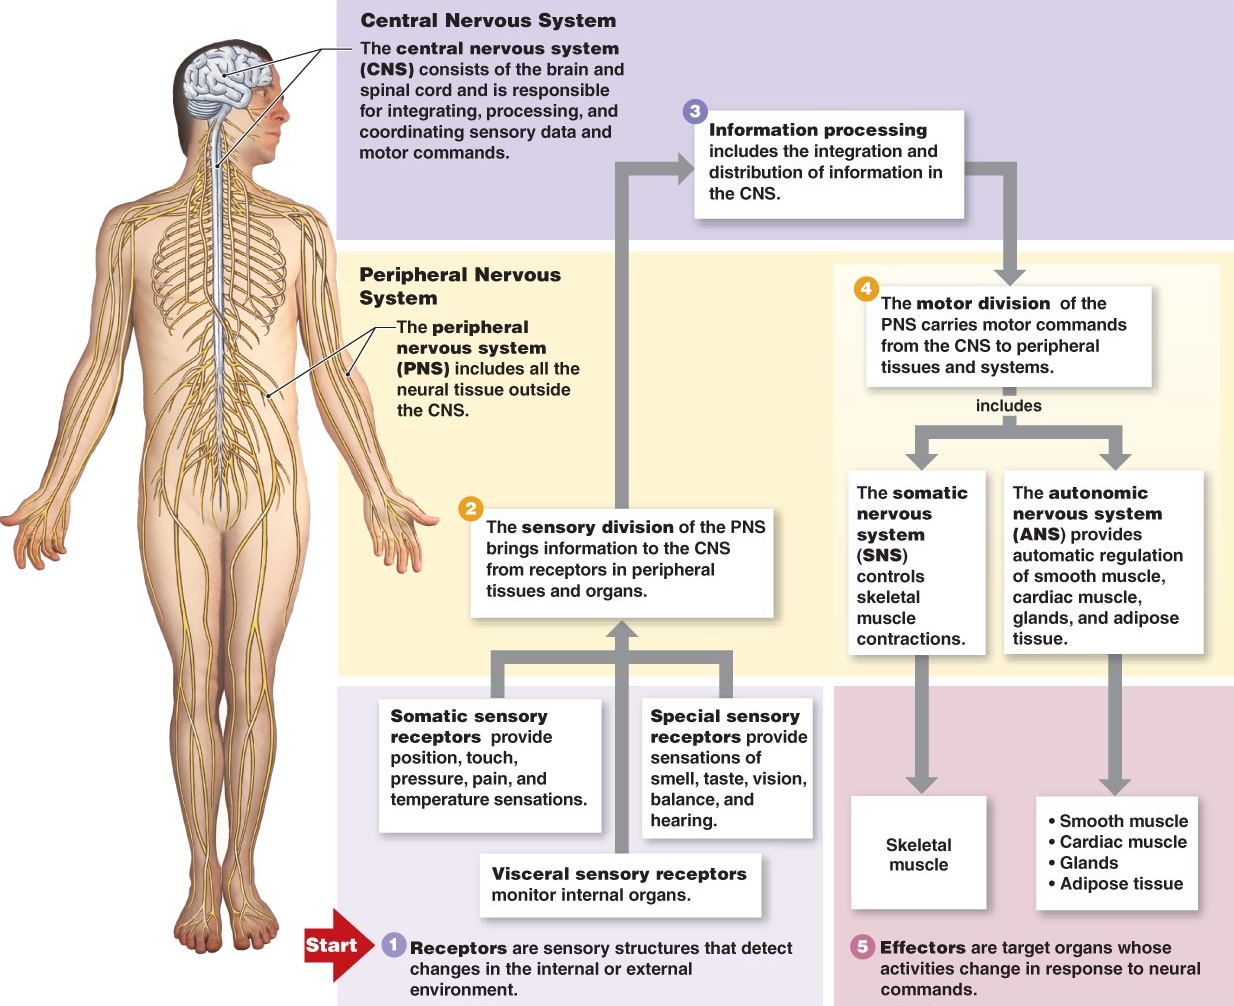
\includegraphics[scale=0.8]{figures/bProblemanalyse/Nervesys.jpg}
	\caption{Her ses et flowdiagram over, hvad der sker, når kroppen modtager et signal og skal processere dette om til en handling. Der ses desuden også en inddeling af CNS pg PNS med dets underdelinger. \cite{2015}}
	\label{Nersys}
\end{figure}

\section{Hjernens anatomi}
Cerebrum er encephalons største del og er involveret i sanseintegration, styring af frivillige bevægelser og højere intellektuelle funktioner, såsom tale og abstrakt tænkning. \cite{Academic2015b} Cerebrums ydre lag hedder cerebral cortex men kaldes hjernens grå substans. Her ligger nervers soma med dendritter. Cerebral cortex har forskellige centre, men kan også inddeles i højre og venstre halvdel. Delen af cerebral cortex der kontrollerer kroppens motorik med motor cortex kaldes gyrus præcentralis. Nerverne i dette område leder motoriske impulser til kroppens muskler igennem nervebanerne i den hvide substans, som indeholder nervernes axoner og fungerer derved som transportvej. \cite{Academic2015b,Martini2012,Stanfield2014} Disse axoner krydses i medulla oblongata og medulla spinalis og løber derefter til det modsatte legemeshalvdel fra, hvor impulsen afsendes. \cite{Martini2012}

	% !TeX spellcheck = da_DK
\chapter{Kroppens balance}\label{app-Balance}
%Apopleksipatienter oplever ofte problemer med balancen, da den ofte er nedsat eller slet ikke funktionsdygtig af forskellige årsager. \cite{Karnath2003} 
Proprioceptorer og sansereceptorer hjælper kroppen med balancen. Proprioceptorerne kontrollerer muskler, sener og leddenes position, hvorimod sansereceptorer er en bestemt slags celler, som f.eks. er placeret i ørerne og øjnene. \cite{Martini2012} Disse celler sender balanceinformationer til CNS og encephalon. Sansereceptorerne opfanger indtryk fra sanserne, som omsættes til bestemte signaler, der sendes til områder i cerebral cortex, cerebellum og centre i hele hjernestammen. Her bearbejdes informationen, hvorefter den korrekte fysiske position af kroppen og dens lemmer konkluderes. Når encephalon har bearbejdet indtrykkene, udsender den nerveimpulser til skeletmuskulaturen om at foretage jævne og koordinerede bevægelser, hvorved kropsbalancen opretholdes.\cite{Martini2012}

Øjet opfanger lys og er med til orienteringen af kroppen og dens lemmer. Hårceller i øret registrerer f.eks. hovedets bevægelser vha. tyngdekraften. Selvom et balanceorgan er ude af funktion, er kroppen stadig i stand til at opretholde balancen ved hjælp fra andre balanceorganer. Det er til gengæld vanskeligt for kroppen at opretholde balancen, hvis de behandlende centre i encephalon bliver skadet, som det kan ske ved apopleksipatienter. \cite{Martini2012} \\

\section{Ørets bidrag til balancen}
Øret består overordnet af tre dele; det ydre øre, mellemøret og det indre øre, som kan ses på \figref{Oeret}. 
\begin{figure}[H]
	\centering
	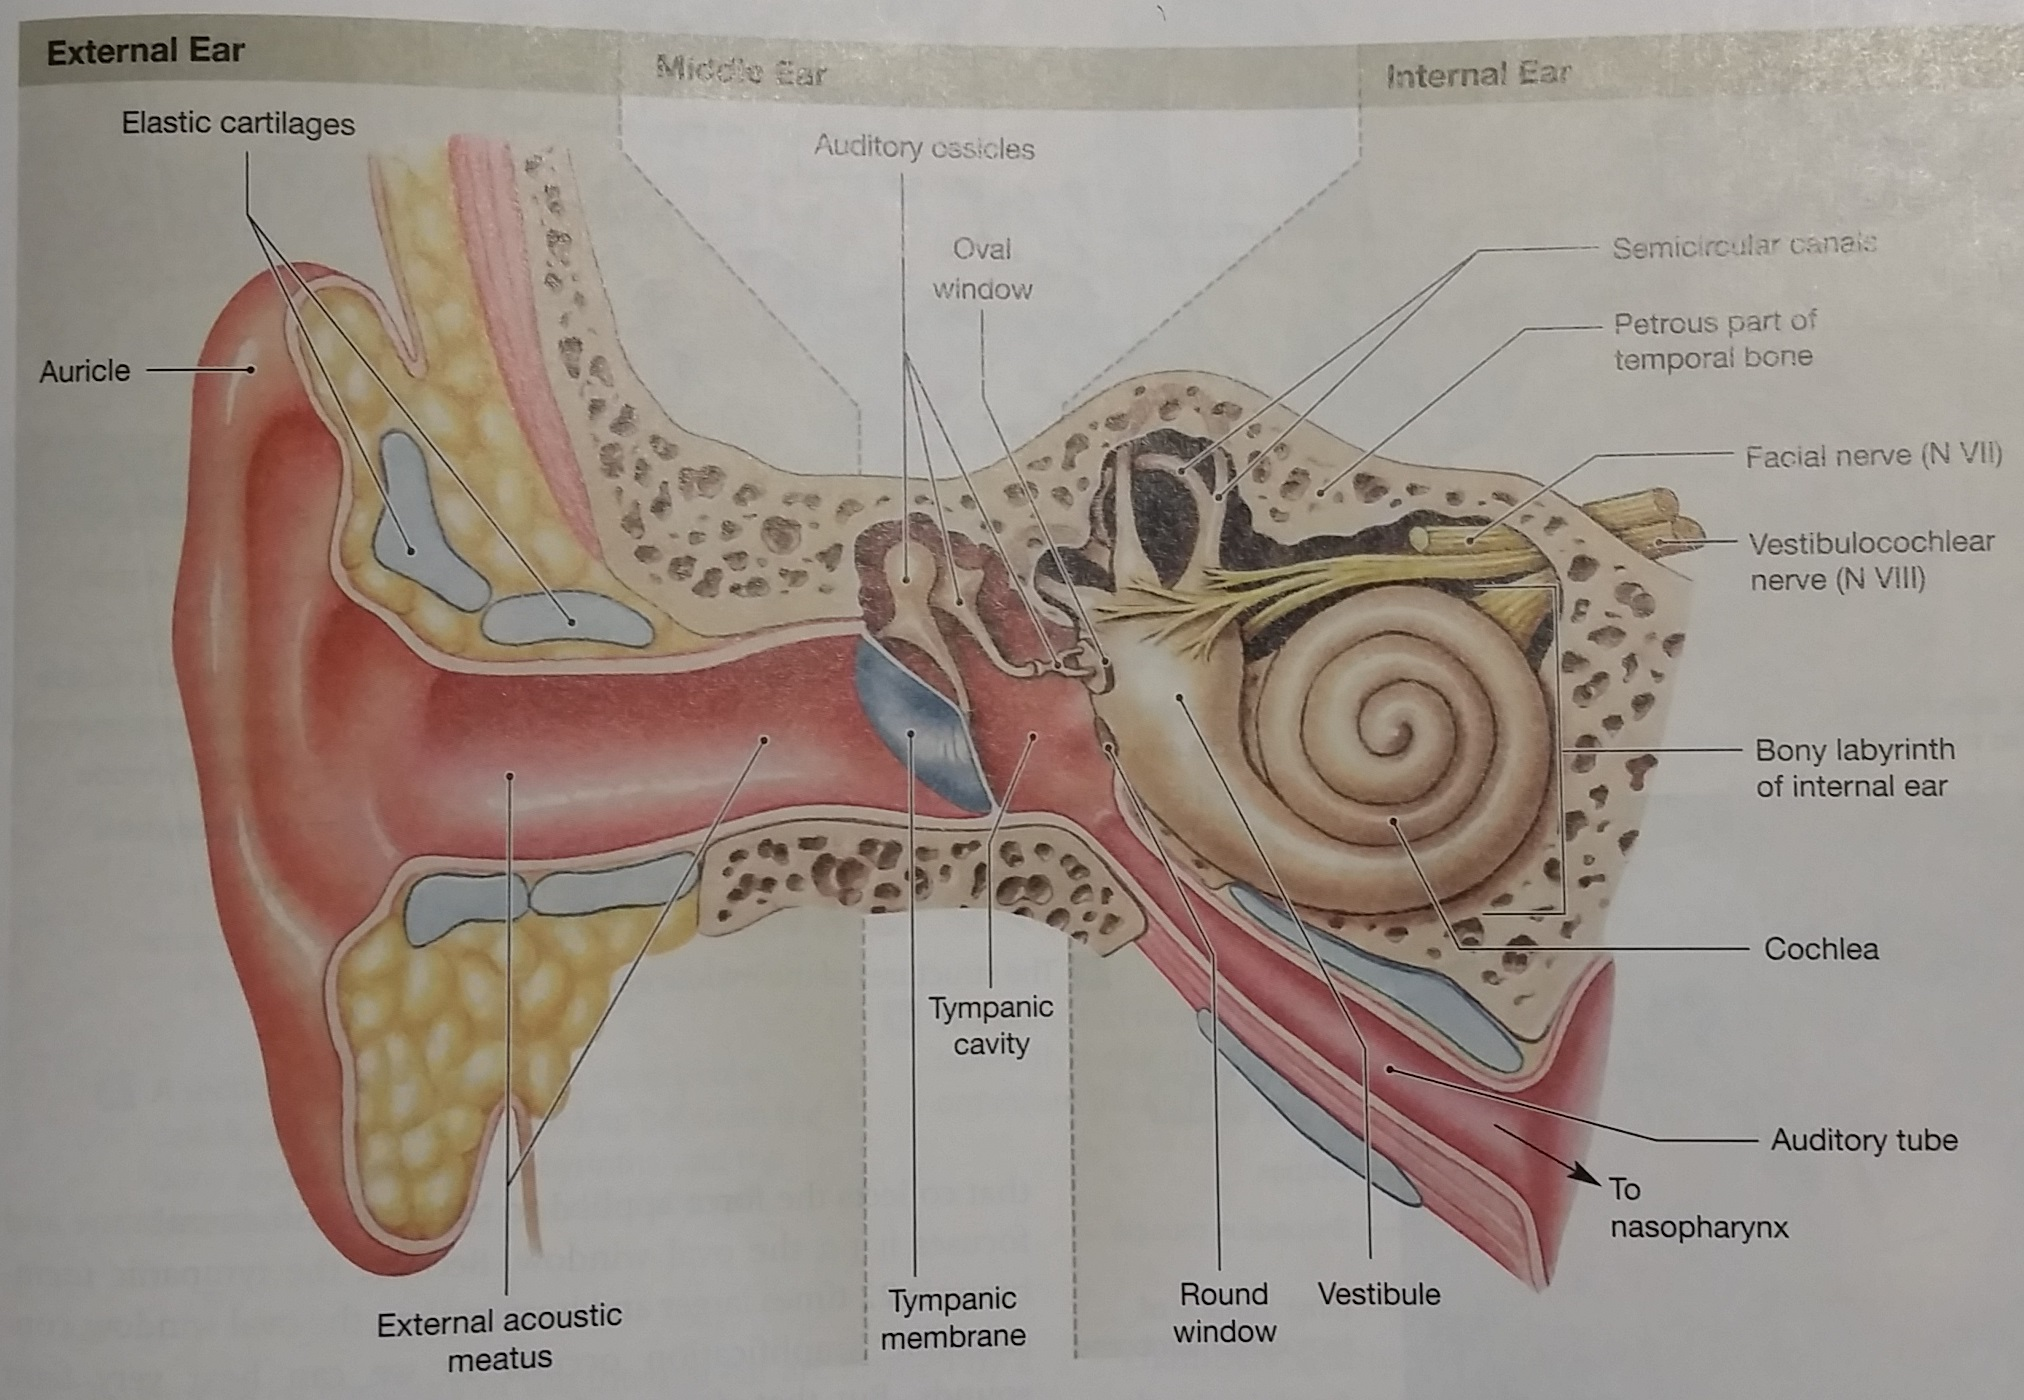
\includegraphics[scale=0.75]{figures/bProblemanalyse/Oerets-anatomi.jpg}
	\caption{På figuren ses ørets anatomiske opbygning \cite{Martini2012}.}
	\label{Oeret}
\end{figure}
Det indre øre er med til at kontrollere balancen vha. hårcellerne, som sættes i bevægelse. Det ydre øre modtager trykbølger, som sætter trommehinden i svingninger. Disse transporteres af mellemørets knogler, der forstærker svingningerne. Væsken i mellemøret modtager svingningerne fra knoglerne, hvilket sætter væsken i bevægelse. Denne bevægelse trækker i hårcellerne, og der skabes derved et aktionspotentiale. I det indre øre findes et netværk af sammenhængende væskeholdige kanaler, som er indkapslet i knoglen. Det er i disse kanaler receptorerne sidder. Det indre øre kan opdeles i tre undergrupper; vestibulen, øresneglen og buegangen. De centrale dele, der er relateret til balancen, er vestibulen og buegangen, hvorimod øresneglen kun bidrager til hørelsen. \cite{Martini2012}

Vestibulen består af to membransække; sacculen og utriclen, der opfanger sanseindtryk vedrørende tyngdekraft og lineær acceleration. Buegangens sansereceptorer opfanger stimuli omkring hovedets bevægelse, og hvor hurtigt bevægelsen foregår. Sansereceptorerne er placeret i buegangens tre væskefyldte knoglekanaler ved ampulla, der er forbundet til utriclen. Hårcellerne er kun aktive, når kroppen er i bevægelse ved at videregive information vedrørende hovedets bevægelse ift. tyngdekraften. Når hovedet er i bevægelse, sættes væsken i kanalerne også i bevægelse således, at væskebevægelser i den ene retning stimulerer hårcellerne, mens bevægelser i den modsatte retning forhindrer dem. For at få mest mulig information angående hovedets position, stimuleres de tre buegange af forskellige hovedbevægelser. Bevægelsesinformationerne sendes via vestibulocochlearnerven, der sender både information vedrørende balancen og hørelsen til encephalon i området mellem pons og medulla oblongata. \cite{Martini2012}    

\section{Øjets bidrag til balancen}
Synet er en central faktor for, hvordan encephalon holdes informeret omkring kroppens balance og generelle orientering. Dette gøres ved at give et indtryk af, hvordan kroppen og dens lemmer er placeret ift. omgivelserne. \cite{Schulmann1987} Øjet har tre hinder; fibrøs hinde, uvea og retina, som kan ses på \figref{Oejet}.
\begin{figure}[H]
	\centering
	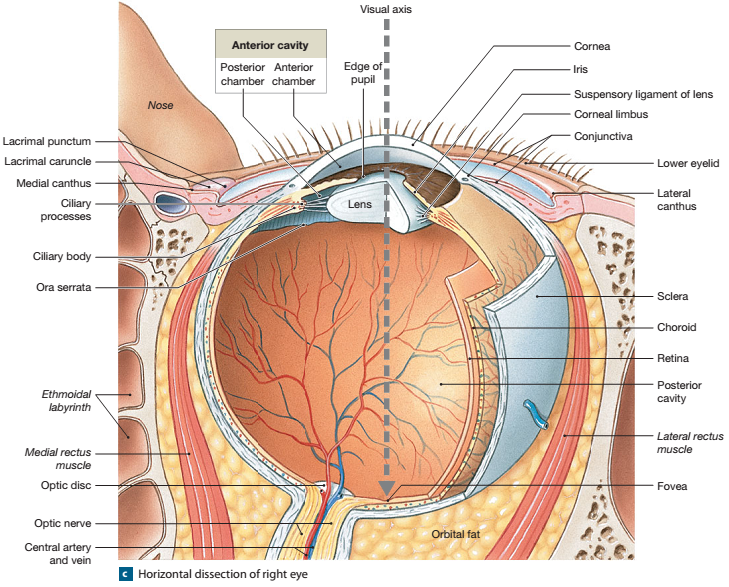
\includegraphics[scale=0.75]{figures/bProblemanalyse/Oejets-anatomi.png}
	\caption{På figuren ses øjets anatomisk opbygning. \cite{Martini2012}}
	\label{Oejet}
\end{figure}
Den fibrøse hinde\fxnote{NTK: hornhinden} er den yderste, som beskytter og støtter øjet. Den midterste hinde, kaldet uvea, indeholder blod og lymfekar samt regulerer mængden af lys, der kommer ind i øjet. Retina\fxnote{NTK: nethinden} er den inderste hinde, som er placeret bagerst i øjet. Den består af en pigmentdel og en indre neuraldel. Den neurale del indeholder fotoreceptorer, bestående af stave og tappe. Stave er følsomme overfor skarpt lys og gør det muligt at se i mørke. Tappe er følsomme overfor farvers bølgelængde, hvilket giver farvesyn. Pigmentdelen absorberer lys, der passerer gennem den neurale del og gør, at lyset ikke har mulighed for at reflektere tilbage. Foto- og lysreceptorerne konverterer lyset fra omgivelserne til elektrisk nervesignal, der giver information omkring det objekt, der betragtes, herunder dets størrelse, form og bevægelser. Informationerne processeres således, at horisontale celler lokaliserer områdets størrelse. Hvis der er kommet tilstrækkeligt med lys ind, sendes informationen først til bipolære celler herefter via synsnerven til det visuelle cortex, hvor informationen bearbejdes. \cite{Martini2012}     

\section{Proprioceptorerne og skeletmuskulaturens bidrag til balancen}
Proprioceptorer monitorerer leddenes position, muskelkontraktioners tilstand, samt spændingen i ledbånd og sener. Disse er placeret i skeletmuskulaturen. Informationerne sendes via nervesignaler til medulla spinalis og herfra igennem CNS til cerebellum. Proprioceptorer inddeles i tre overordnet grupper; muskelspindlere, golgi-sene organer og receptorer i ledkapsler. \cite{Martini2012}

Muskelspindlere styrer og kontrollerer ændringer af muskellængder og kan udløse en strækrefleks. Den sensoriske nerve er forbundet centralt på muskelspindleren, hvor den kontinuert sender sensoriske impulser til CNS. Hvis den sensoriske nerve modtager stimuli, i form af stræk, vil den motoriske nerve på muskelspindleren blive stimuleret. Stimulation af den motoriske nerve vil forkorte musklens længde. Nogle strækreflekser er holdningsreflekser, som hjælper til at holde balancen. I stående position kræves der et samarbejde mellem forskellige muskelgrupper for at forblive stående. Dette ses f.eks. hvis kroppen lænes forover, vil strækreflekserne i læggene blive aktiveret og kontraherer. Derved vil kroppen læne sig bagud og igen stå i en opret position. Hvis der sker en overkompensation fra lægmusklerne og kroppen læner sig for meget bagud, vil strækreflekser i skinnebenet og lårene aktiveres. Derved vil kroppen læne sig forover igen. Kroppen foretager mange af disse ubevidste korrektioner. \cite{Martini2012}   %(Se Martini 9th side 438 under "monosynaptic reflexes")

Golgi-sene organer sidder i en kløft\fxnote{NTK: kaldes junction på engelsk} mellem skeletmusklen og tilhørende sene. Dendritterne fra golgi-sene organet kobler sig på den nærmeste sene og stimuleres af spændingen i denne, hvorved den eksterne spænding i en muskelkontraktion bliver målt. \cite{Martini2012} 

Ledkapsler er fyldt med frie nerveender, som kaldes receptorer. Disse receptorer detekterer tryk, spænding og bevægelse i leddet. \cite{Martini2012}    \\
Det er en lille del, af den information proprioceptererne sender, der opfanges af bevidstheden, eftersom størstedelen foregår på et underbevidst niveau. \cite{Martini2012} \\


%Golgi seneorganer (Se Martini 9th side 501 under 15-3 propriocetor) %Receptorer i ledkapsler (Se Martini 9th side 501 under 15-3 propriocetor)

%\subsection{Apopleksi og balance}
%Balancen er styrer flere steder i kroppen og er med til at beskytte kroppen mod f.eks. faldulykker, ved at sikre at kroppen og den lemmer bevæger sig i kontrollerede og jævne bevægelser. Kroppen opretholder balancen ved at bruge ørerne, øjne og proprioceptorer i skeletmuskulaturen. Proprioceptorerne kontrollerer muskler, sener og leds position. Øjne opfanger lys og er med til orienteringen af kroppen og dens lemmer og hårceller i øret register hoveds bevægelser ved hjælp af tyngdekraften. Selvom et balanceorgan er ude af funktion er kroppen stadig i stand til at opretholde balancen ved hjælp fra andre balanceorganer. Det er til gengæld svære for kroppen at opretholde balancen hvis centrene i hjerne, som behandler den information, som kommer fra balanceorganerne, bliver skadet, som det kan ske ved apopleksi patienter. \cite{Martini2012}
% [1] – Martini, Frederic H and others. Fundamentals of Anatomy & Physiology (Kapitel:13, 14, 15, 17 ). 2012. Pearson. 
% [2] - Karnath2003
	% !TeX spellcheck = da_DK
\chapter{Pilotforsøg}\label{Bilag:Pilotforsoeg}
Det er nødvendigt at kunne skelne det reelle signal fra støjkomponenter, før systemet kan designes. Signalet skal aktivere komponenter i slutningen af det analoge system og skal derfor være adskilt fra støj, der kan påvirke outputtet. For at undgå dette frafiltreres støjsignaler. Derudover er det nødvendigt at vide, hvilket outputsignal accelerometeret giver ift. den valgte hældningsgrad. Dette gøres ud fra sensitiviteten, der måles. Ud fra disse oplysninger er det muligt at kravspecificere de enkelte blokke i systemet. \\ % Oplysningerne findes på baggrund af et pilotforsøg.
Accelerometerets datablad informerer om, at der skal benyttes Kapacitorer til opsamling af signalet. Kapacitorens størrelse (C) beregnes ud fra følgende formel fra \cite{Devices2009}:
\begin{equation}
\text{Båndbredde} = \dfrac{5\mu F}{C} \Rightarrow  C = \dfrac{5\mu F}{\text{Båndbredde}}
\end{equation}
Frekvensområdet for kropshældning er ikke klart defineret, men studier anvender et frekvensområde liggende mellem $0.02-10Hz$ \cite{Martinez-Mendez2011}. Grundet usikkerheden vælges en båndbredte på $50$Hz, hvilket gør, at C bliver $0.1\mu$F.

\section{Formål med pilotforsøg}
\begin{enumerate}
\item Identificere de frekvenser, der udgør støj i outputsignalet fra accelerometeret.
%\item Udregner accelerometerets g-påvirkning ved $8^{\circ}$ og $13^{\circ}$.
\item Identificere maksimum og minimum outputsignal af accelerometeret.
\item Kontrollere om offset og sensitivitets værdierne fra databladet på accelerometeret stemmer overens med målt data.
\end{enumerate}

\section{Materialer}
\begin{itemize}
\item ADXL335 accelerometer.
\item To stk. $0.1\mu$F kondensatorer.
\item en stk. TL081 operationsforstærker
\item Ledninger.
\item Breadboard.
\item $5.5V$ fra spændingsforsyning fra batterier.
\item NI USB-6009.
\item USB isolator USI-01.
\item Computer med ScopeLogger og MATLAB R2015a.
\item Hæftemasse.
\item Vinkel.
\item Vaterpas.
\item Termometer
\end{itemize}

\section{Metode}
\begin{enumerate} [label=\bfseries Formål \arabic*:]
\item Støjfrekvenserne i outputsignalet identificeres ved først at måle en baseline ved $0g$ dvs. uden hældning. Dette medfører at signalet kan analyseres uden nogen påvirkning på outputsignalet. Dernæst måles en påvirkningen ved $1$g, hvilket svarer til en hældning på $90^{\circ}$. Dette måles både til højre og venstre. Derudover udføres en langsom rotation fra $0^{\circ}$ til $90^{\circ}$ til både højre og venstre. Det vil på denne måde være muligt at identificere den støj som accelerometeret kan udsættes for. %Det samme gøres for de specificerede hældningsgrader, som er $8^{\circ}$ og $13^{\circ}$. 
\item For at simulere den påvirkning, accelerometeret udsættes for, og derved identificere accelerometerets maksimum og minimums outputsignal, roteres accelerometret i en langsom rotation fra $0^{\circ}$ til $90^{\circ}$ til både højre og venstre.
\item På baggrund af identificering af de forrige formål samt ved måling af temperaturen i lokalet før, under og efter, kontrolleres temperaturens indvirkning på accelerometerets sensitivitet samt om de forrige formål stemmer overens med værdierne fra databladet på accelerometeret. \cite{Devices2009} 
\end{enumerate}
%Støjfrekvenserne i outputsignalet identificeres ved først at måle en baseline ved $0g$ dvs. uden hældning. Dette medfører at signalet kan analyseres uden nogen påvirkning på outputsignalet. Dernæst måles en påvirkningen ved $1$g, hvilket svarer til en hældning på $90^{\circ}$. Dette måles både til højre og venstre. Derved kan det sammenlignes, om der er støj ift. baseline. %Det samme gøres for de specificerede hældningsgrader, som er $8^{\circ}$ og $13^{\circ}$. 
%For at simulere den påvirkning, accelerometeret udsættes for og identificere den mulige støj ved en rotation, roteres accelerometret i en langsom rotation fra $0^{\circ}$ til $90^{\circ}$ til både højre og venstre. Disse målinger vil identificere minimum og maksimum outputsignal, som accelerometeret kan afgive i dette tilfælde, samt kontrollere om offset og sensitivitet informationerne fra accelerometerets datablad stemmer overens med det målte data. \\
%Inden, under og efter forsøget måles temperaturen i lokalet, da denne kan have en effekt på accelerometerets sensitivitet. \cite{Devices2009}

\subsection{Forsøgsopsætning}
Opsætningen er udarbejdet både i LTspice og på breadbord \ref{pforsoeg1}. Opsætningen af pilotforsøget i LTspice  er illustreret i et billede \ref{pLTspice} og er udarbejdet på baggrund fra målte værdier udregnet i pilotforsøget. Opsætningen på breadbord er udarbejdet ud fra protokolen under \ref{Opsaetning}.  

\begin{figure}[H]
		\centering
		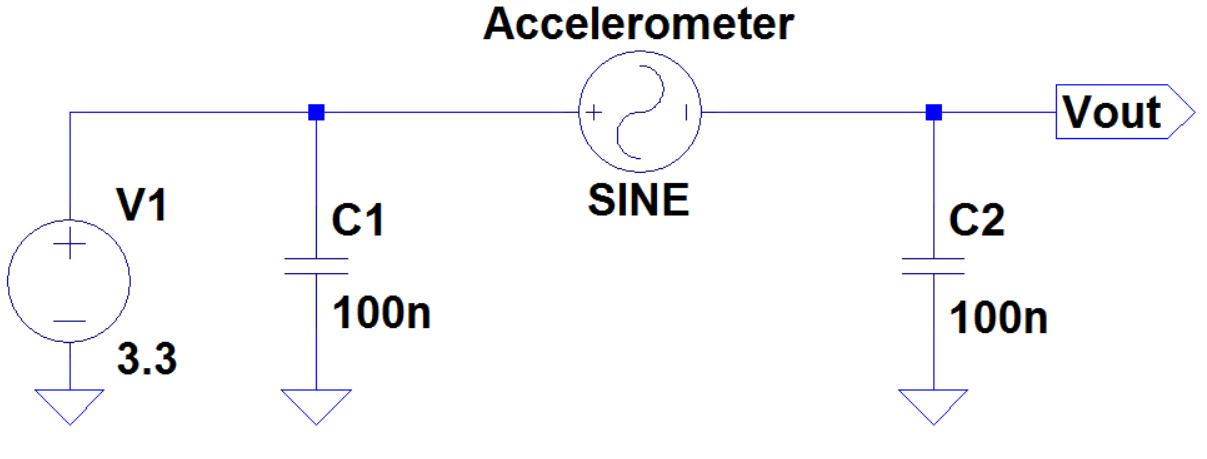
\includegraphics[scale=0.4]{figures/Bilag/Test_opsaetning.PNG}
		\caption{På figuren ses opsætningen i LTspice. Accerometeret er symboliseret med en sinuskurve med et DC offset svarende til den tilførte strømforsyning fratrukket offsettet fra accelerometeret ved $0$g påvirkning. Derudover angivet en amplitude svarende til den maksimale sensitivitet for accelerometeret, som findes i dette forsøg.}
		\label{pLTspice}
\end{figure}

\noindent Outputtet fra accelerometret har en høj outputimpedans, hvorfor der indsættes en buffer. En buffer er et elektroniske kredsløb, hvis primære funktion er at forbinde en kilde med høj outputimpedans til en anden kilde med lav indgangsimpedans uden væsentlig dæmpning eller fordrejning af signalet. Outputimpedansen fra bufferen vil alts være lav, og derfor vil koblingen imellem den forrige blok og den være mulig uden påvirkning - i dette tilfælde af signalet fra accelerometret. Der benyttes en operationsforstærker TL081 i en ikke konverterende konfiguration og med et gain på $1$.\cite{Schaumann2014} Dette ses på \figref{fig:Buffer}.
\begin{figure}[H]
	\centering
	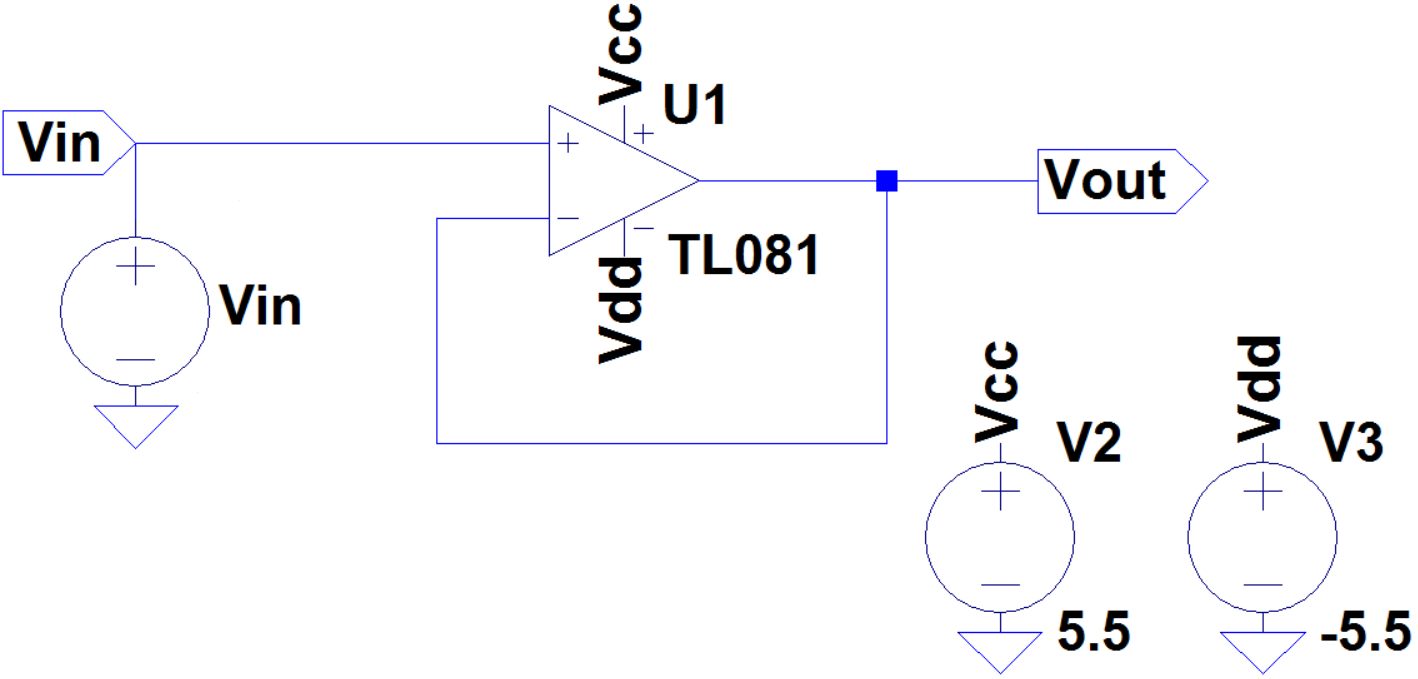
\includegraphics[scale=0.4]{figures/cProblemloesning/Buffer_LT.png}
	\caption{På figuren ses en buffer, som fungerer som en forstærker med et gain på faktor 1.}
	\label{fig:Buffer}
\end{figure}

\textbf{Opsætning}\label{Opsaetning}
\begin{itemize}
\item Accelerometeret tilkobles breadboardet.
\item De to kondensatorer på tilkobles breadboardet. Kondensatorererne er valgt på baggrund af databladet for acceleorometeret ift. power supply decoupling og båndbredde. $0.1\mu$F kondensatoren, som sidder på pin $1$ og $2$ i accelerometeret, fjerner støj fra strømforsyningen, mens kondensatoren fra pin $3$ på $0.1\mu$F giver en båndbredde på $50Hz$. Målingerne af disse ses i \tableref{Tab:Acc_kondensator}.
\item Accelerometeret tilnyttes en forsyningsspænding på $5.5V$ - en regulator sikrer at accelerometret kun forsynes med en spænding indenfor dets arbejdsområde, som er $3.3$V.
\item En buffer designes med en operationsforstærkeren TL081 og en ledning fra den inverterende kanal til outputkanalen. Derved påvirker indgangsimpedansen fra ADC'en af typen NI USB-6009 ikke signalet fra accelerometret.\fxnote{Modstanderen i NI USB-6009 er 144Kohm er ikke 100 gange større end den 32Kohm fra accelerometret. derfor påvirker det sifnalet.}
\item Outputtet fra bufferen sendes igennem en ADC af typen NI USB-6009.
\item Signalet fra NI USB-6009 sendes igennem en USB-isolator af typen USI-01.
\item Outputsignalet fra USI-01 sendes ind i computeren, hvor det optages med ScopeLogger og behandles i MATLAB R2015a.
\end{itemize}

\noindent De to kapacitorer blev målt inden implementering samt den samlede kapacitans. Resultaterne fremgår i  \tableref{Tab:Acc_kondensator_pilot}:
\begin{table}[H]
	\centering
	\begin{tabular}{|l|l|l|l|}\hline
		& \textit{Teoretisk} & \textit{Målt} & \textit{\% afvigelse} \\ \hline
		\textit{C1}       & \textit{$0.1\mu$F} & $0.1004\mu$F  & $0.4\%$               \\ \hline		
		\textit{C2}       & \textit{$0.1\mu$F} & $0.1009\mu$F  & $0.9\%$               \\ \hline
	\end{tabular}
	\caption{I tabellen ses det, at de to kondensatorer afviger lidt fra deres teoretiske værdi, hvilket er forventet af reelle komponenter.}
	\label{Tab:Acc_kondensator_pilot}
\end{table}

\noindent På \figref{pforsoeg1} ses den endelige forsøgsopsætningen.
\begin{figure}[H]
	\centering
	\includegraphics[scale=0.4]{figures/Bilag/Acc_medbuffer.png}
	\caption{På figuren ses designet af pilotforsøget i LTspice.}
	\label{pforsoeg1}
\end{figure}

\section{Fremgangsmåde}
\subsection{Forsøgets udførelse}
Hele pilotforsøgets opsætning ses på \figref{pforsoeg2}. \\
For at måle $0g$ påvirkning på accelerometerets x-akse, lægges det fladt ned på et plant bord, som er tjekket med et vaterpas. Målingen gøres over tre omgange i $30$ sekunder. Herefter holdes accelerometeret fast på en vinkel, hvor ledningerne påsættes med hæftemasse. Accelerometeret sættes så der igen måles på x-aksen, når der sker en rotation til højre og venstre. Vinklen sættes således, at der måles $1g$ påvirkning i positiv retning og negativ retning, hvilket svarer til $\pm90^{\circ}$ fra accelerometerets nulpunkt. \\
Dette giver tre baselines for hver g påvirkning, som opsamles og gemmes i ScopeLogger. %Herudover måles en baseline for g påvirkningen af accelerometeret ved $8^{\circ}$ og $13^{\circ}$. Dette gøres ved at holde accelerometeret i 30 sekunder på $8^{\circ}$ og $13^{\circ}$ henholdsvis til højre og venstre. Herved fås 4 baselines, som optages og gemmes i ScopeLogger. 
Til sidst måles g påvirkningen af accelerometeret under rotation fra $0^{\circ}$ til $\pm$ $90^{\circ}$ for både højre og venstre. Her måles $10$ sekunders baseline inden og efter rotationen, som varer $5$ sekunder og foretages langsomt og kontrolleret. Disse to målinger optages og gemmes ligeså i ScopeLogger. \\
\subsection{Behandling af data}
Efter udførelse af forsøget vil alt data blive behandlet i MATLAB R2015a, hvor der beregnes en gennemsnitsværdi for henholdsvis de tre baselines målt ved $0g$ påvirkning samt $1g$ påvirkning i positiv retning og negativ retning. Der foretages desuden en Fast Fourier Transformation (FFT) på de ni målinger (tre målinger ved hver g påvirkning). FFT foretages for at få en grafisk repræsentation af det målte signal i frekvensdomænet. Baseline optages for at se hvilken påvirkning omgivelserne har på signalet, da der ikke er nogen bevægelse på disse.

\begin{figure}[H]
	\centering
	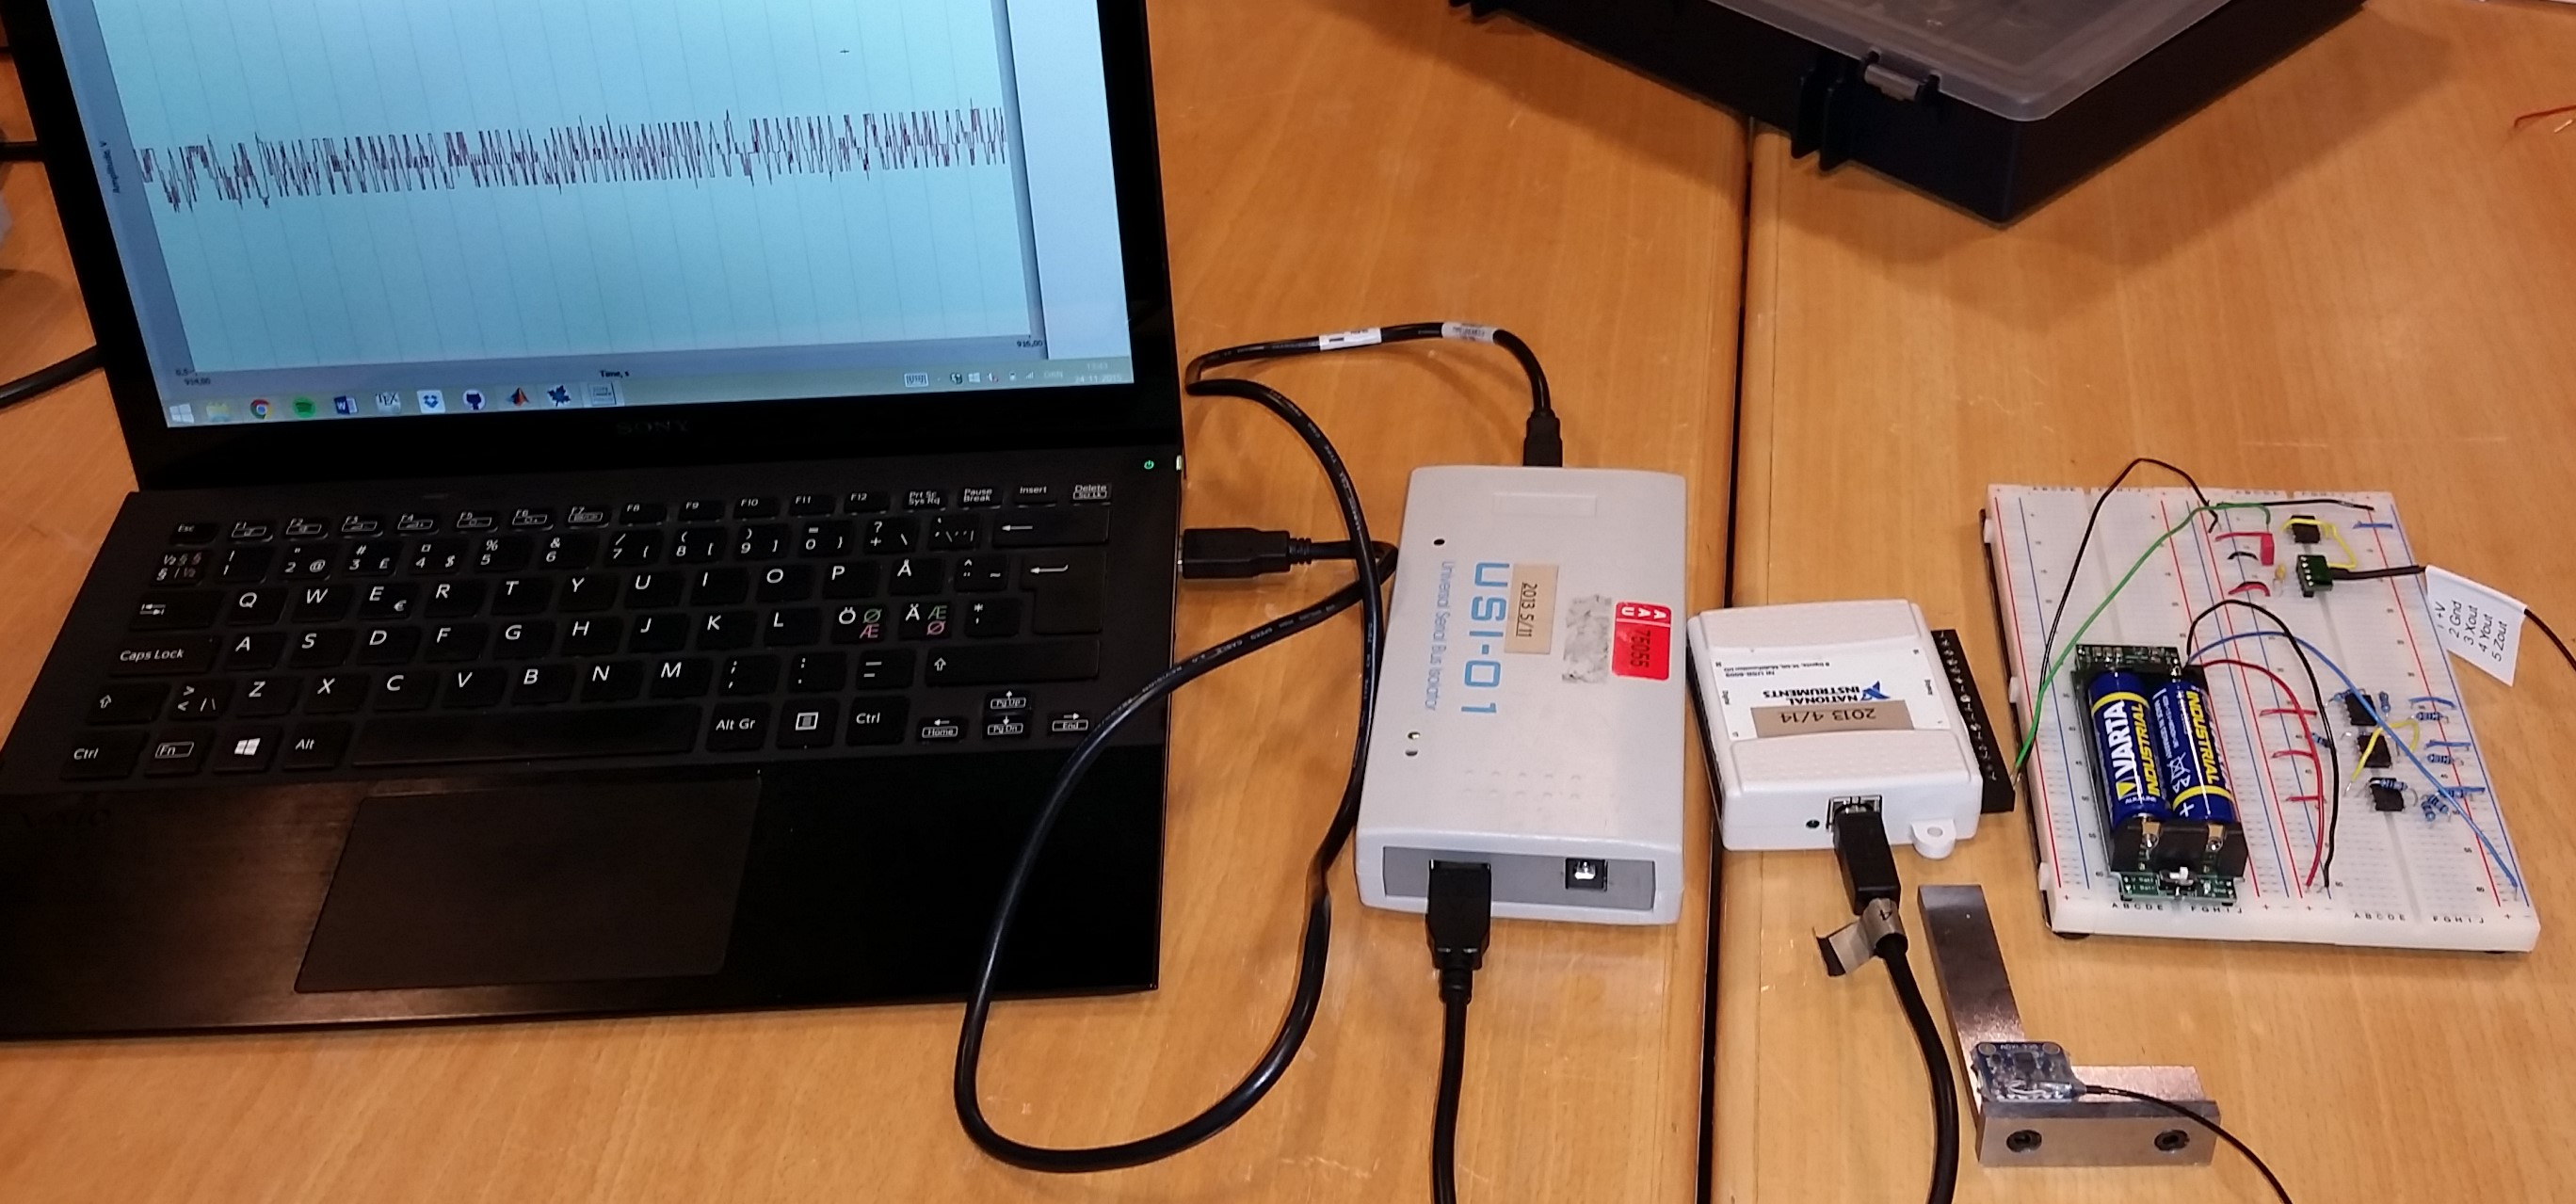
\includegraphics[scale=0.14]{figures/cProblemloesning/Pilotforsoeg1_2.jpg}
	\caption{På billedet ses (fra venstre til højre) den 5V spændingsforsyning, som leder strømmen til og fra ground fra breadboardet. Fra breadboardet sendes outputtet videre til ADC'en(NI USB-6009). Herefter ledes signalet igennem USB-isolatoren(USI-01) og til sidst ind i computeren, hvor det optages i ScopeLogger. Over breadboardet i midten på billedet ses vaterpasset. Forrest i midten på billedet ses accelerometret fastgjort på vinklen.}
	\label{pforsoeg2}
\end{figure}

\section{Resultater}\label{Sec_Pilot_Data}
I dette afsnit vil der grafisk blive vist, hvordan accelerometerets output ændrer sig ift. g påvirkning. På \figref{Fig:Pilot_Tid} ses accelerometerets output i tidsdomænet. Der udføres herefter en FFT på de tre målinger for hver baseline, hvilket giver ni grafiske skiltninger af, hvorledes accelerometerets egne frekvenser adskiller sig fra støjfrekvenser.

\begin{figure}[H]
	\centering
	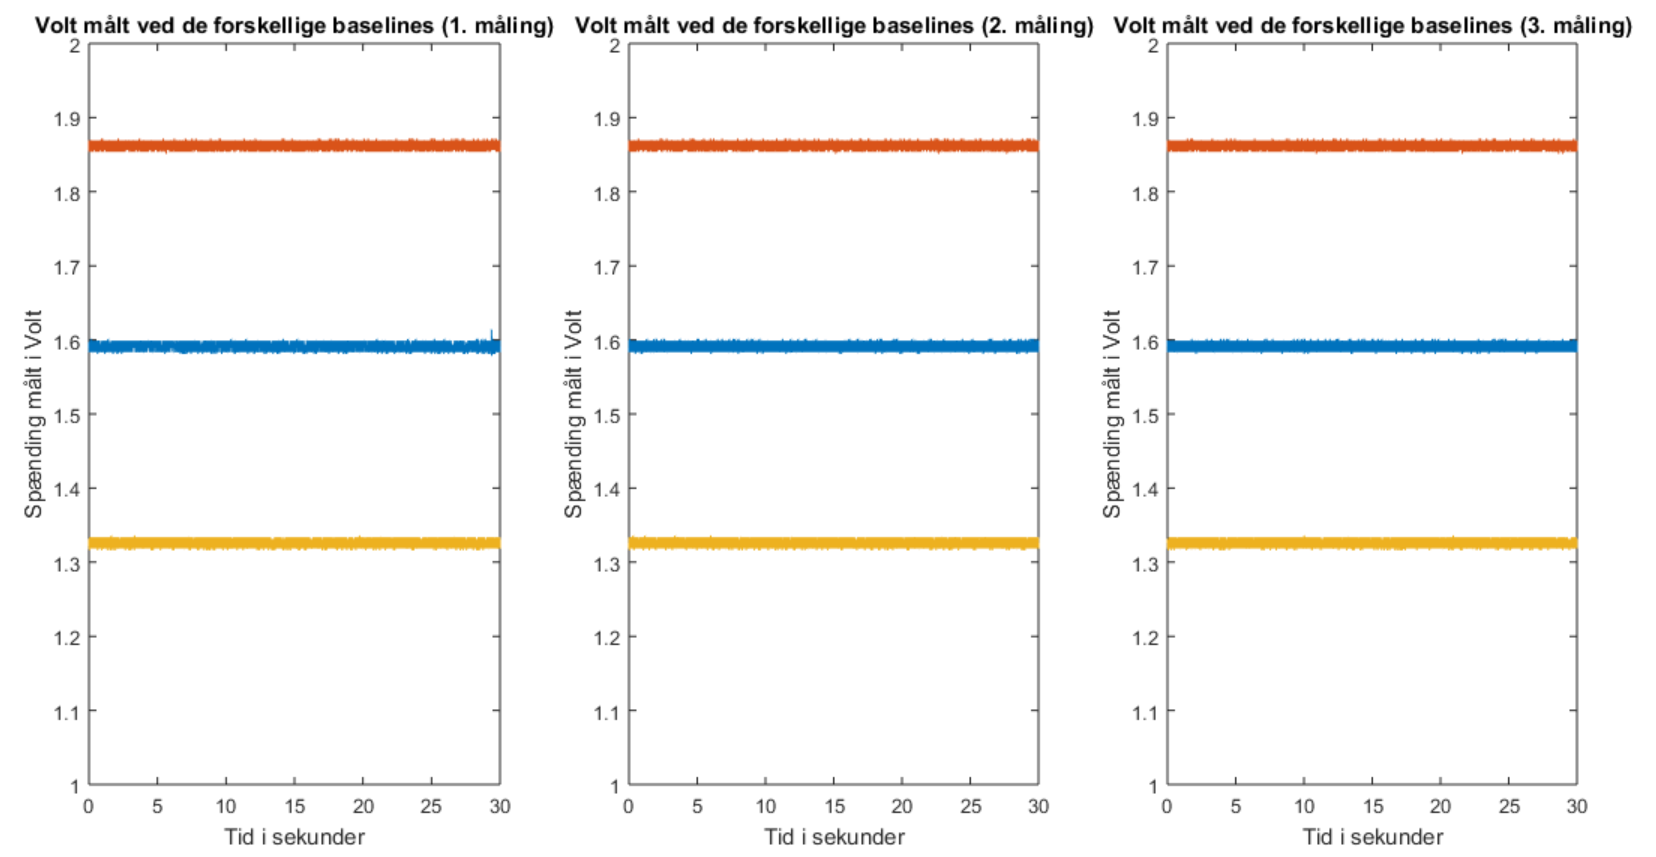
\includegraphics[scale=0.45]{figures/cProblemloesning/Pilotforsoeg_Tid.png}
	\caption{På graferne ses henholdsvis første, anden og tredje måling for hver g påvirkning af accelerometret. Den røde graf repræsenterer outputtet målt ved $1g$ påvirkning i positiv retning. Den blå graf repræsenterer outputtet målt ved $0g$ påvirkning. Den gule graf repræsenterer outputtet målt ved $1g$ påvirkning i negativ retning.}
	\label{Fig:Pilot_Tid}
\end{figure}

Offsettet for accelerometerets x-akse udregnes ved at tage den målte gennemsnitsværdi ved $0$g for alle tre målinger og yderligere tage gennemsnittet af disse. De tre målinger ses som de blå grafer på \figref{Fig:Pilot_Tid}. Udregningen ses på \ref{Mean_tid_0g}:
\begin{equation}\label{Mean_tid_0g}
\text{Offset} = \frac{1.6326 + 1.6323 + 1.6325}{3} = 1.6325
\end{equation}
\noindent Offsettet burde ifølge databladet for accelerometret være halvdelen af spændingsforsyningen, som i dette tilfælde leder en spænding på $3.3V$. \cite{Devices2009} Derfor burde offsettet være $1.65V$. Afvigelsen kan derved udregnes:
\begin{equation}
\text{Afvigelse for offset} = \dfrac{1.6325 - 1.65}{1.65} \cdot 100 = -1.0614\% \approx 1.06\%
\end{equation}

\noindent Herefter kan sensitiviteten for accelerometeret udregnes. Dette gøres ved først at udregne en gennemsnitsværdi for $1g$ påvirkning i henholdsvis positiv og negativ retning. Værdierne for $1$g påvirkning i positiv retning er angivet som de røde grafer på \figref{Fig:Pilot_Tid}, imens de i negativ retning er angivet som de gule grafer. Efter udregningen af gennemsnittet trækkes den udregnede offset værdi fra.
\
\begin{align}\label{taeskelvaerdi_pr_grad}
	\text{Gennemsnit 1g positiv retning} = \frac{1.9640 + 1.9636 + 1.9639}{3} = 1.9638 \\
	\text{Gennemsnit 1g negativ retning} = \frac{1.3091 + 1.3093 + 1.3093}{3} = 1.3092 \\
	\text{Sensitivitet positiv retning} = 1.9638 - 1.6325 = 0.3313 \\
	\text{Sensitivitet negativ retning} = 1.3092 - 1.6325 = -0.3233 \\
	\text{Volt pr grad positiv retning} = \dfrac{0.3313}{90} = 0.0037\text{V} \\
	\text{Volt pr grad negativ retning} = \dfrac{-0.3233}{90} = 0.0036\text{V}
\end{align}
\noindent Da der findes en lineær sammenhæng imellem g påvirkning og outputtet burde sensitiviteten for accelerometret med en spændingsforsyning på $3.3V$ være $330mV/g$. Der kan derved udregnes afvigelse for både negativ og positiv retning:
\begin{align}
	\text{Afvigelse for sensitivitet i positiv retning} = \dfrac{0.3313 - 0.330}{0.330} \cdot = 0.3939\% \approx 0.39\% \\
	\text{Afvigelse for sensitivitet i negativ retning} = \dfrac{0.3233 - 0.330}{0.330} \cdot = -2.0303\% \approx 2.03\%
\end{align}

På \figref{Fig:Pilot_FFT0}, \figref{Fig:Pilot_FFTN} samt \figref{Fig:Pilot_FFTP} ses en FFT af det målte data for statisk acceleration.
\begin{figure}[H]
	\centering
	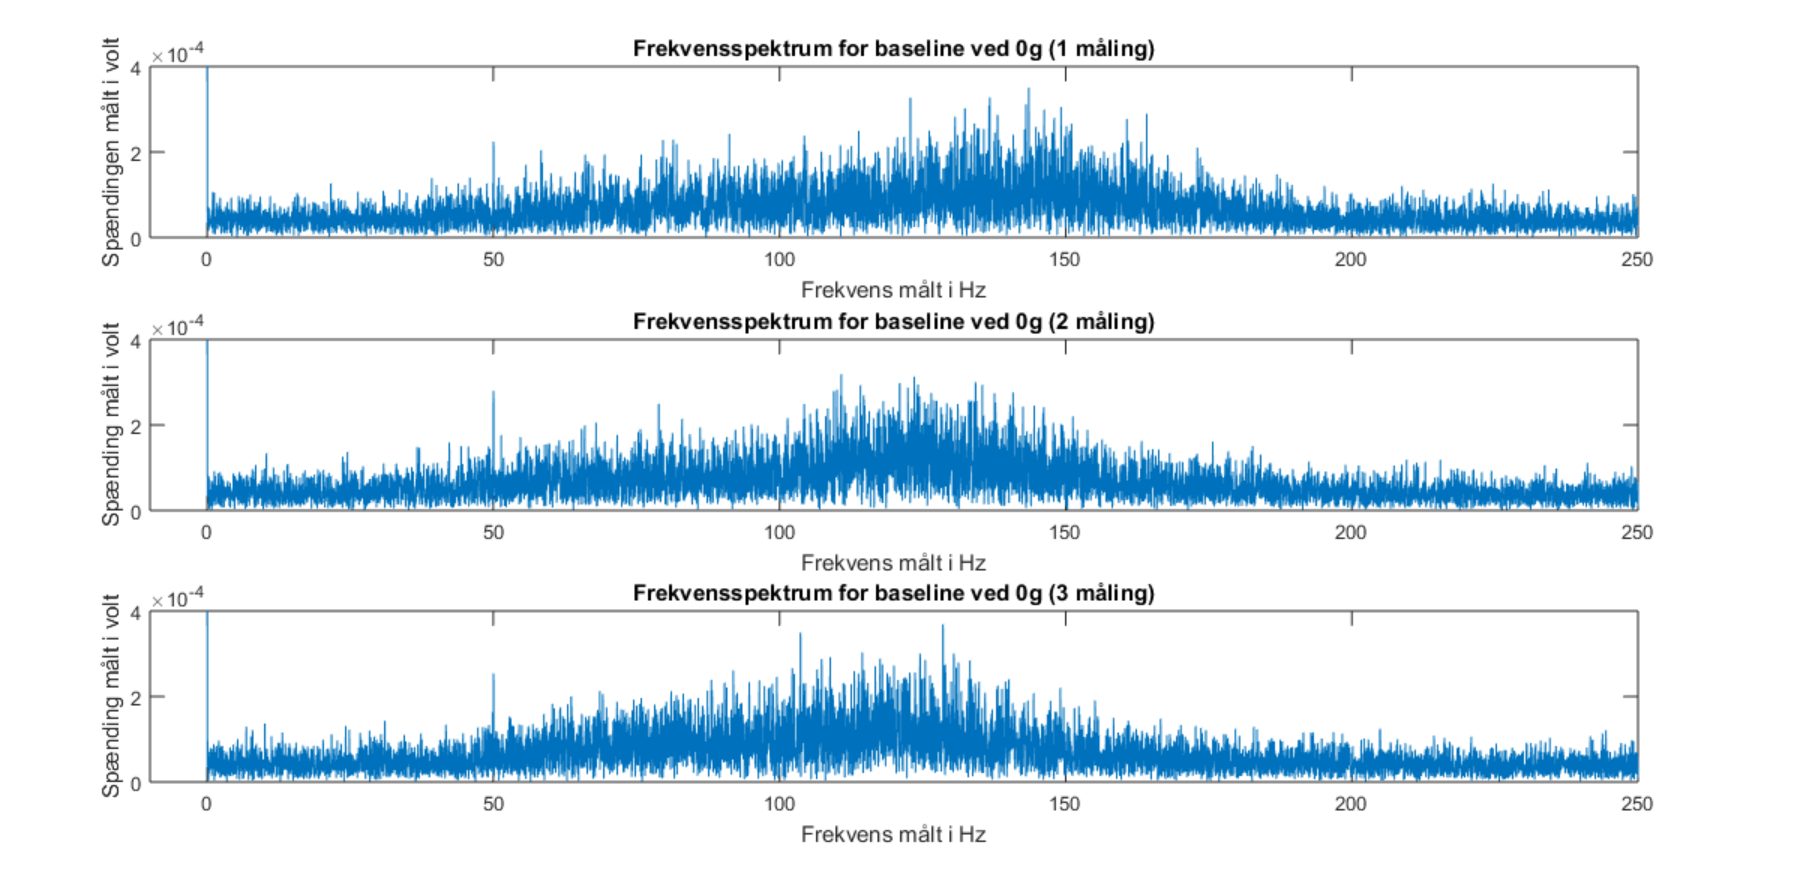
\includegraphics[scale=0.5]{figures/cProblemloesning/Pilotforsoeg_Frekvens0.png}
	\caption{På de tre grafer ses en FFT af første, anden og tredje måling ved $0g$ påvirkning af accelerometret. Peaken ved $0Hz$ går op til ca. $1.63V$ men dette ses ikke på grafen, da resten af værdierne derved vil være meget svære at se.}
	\label{Fig:Pilot_FFT0}
\end{figure}
\begin{figure}[H]
	\centering
	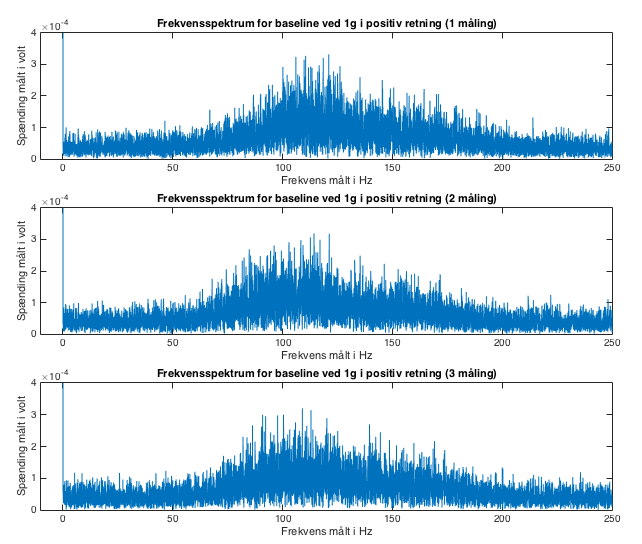
\includegraphics[scale=0.5]{figures/cProblemloesning/Pilotforsoeg_FrekvensP.png}
	\caption{På de tre grafer ses en FFT af første, anden og tredje måling ved $1g$ påvirkning af accelerometret i positiv retning. Peaken ved $0Hz$ går op til ca. $1.96V$, men dette ses ikke på grafen, da resten af værdierne derved vil være meget svære at se.}
	\label{Fig:Pilot_FFTP}
\end{figure}
\begin{figure}[H]
	\centering
	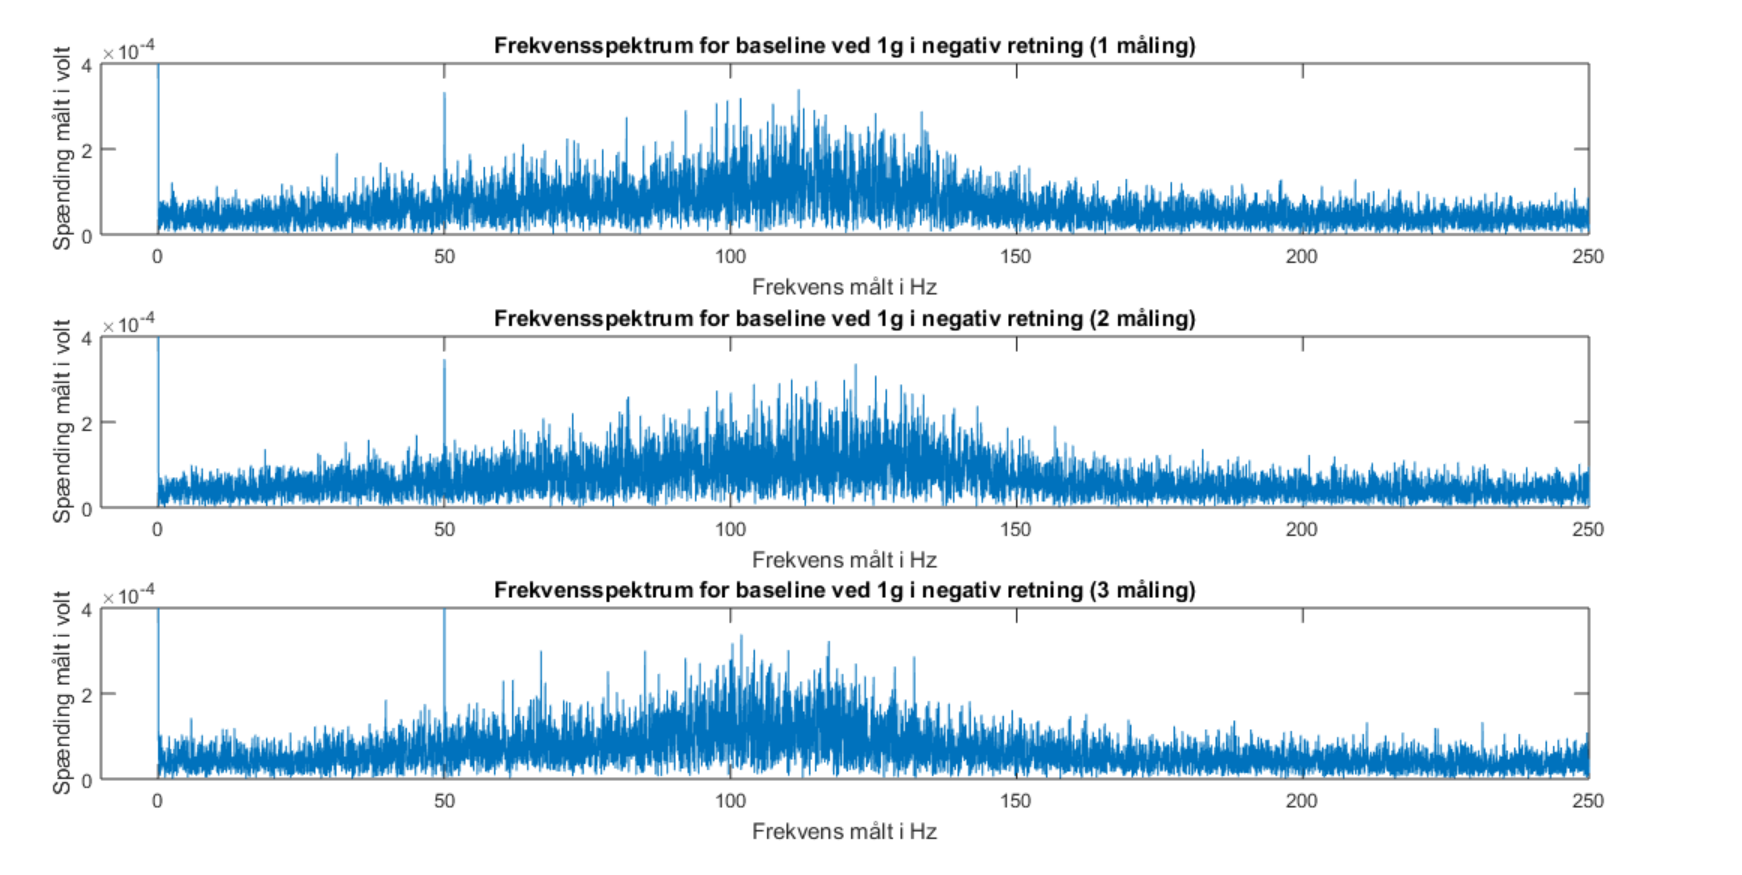
\includegraphics[scale=0.5]{figures/cProblemloesning/Pilotforsoeg_FrekvensN.png}
	\caption{På de tre grafer ses en FFT af første, anden og tredje måling ved -$1g$ påvirkning af accelerometret i negativ retning. Peaken ved $0Hz$ går op til knap $1.30V$, men dette ses ikke på grafen, da resten af værdierne derved vil være meget svære at se.}
	\label{Fig:Pilot_FFTN}
\end{figure}

\noindent Sammenlignes peakværdierne ved $0Hz$ på de tre ovenstående figurer med peakværdierne i resten af signalet fremgår det, at signal to noise ratioen er lav, hvilket betyder, at der ikke er meget støj ift. ønsket signal. Der ses altså, at accelerometerets frekvensområde ligger i de lave frekvenser. Der ses ved en statisk acceleration at, signalet stort set kun er til stede ved $0Hz$. Alt over $0Hz$ betragtes derfor som støj. 

\begin{figure}[H]
	\centering
	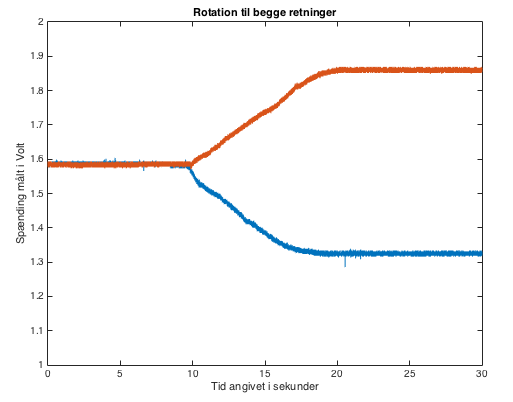
\includegraphics[scale=0.45]{figures/cProblemloesning/Pilotforsoeg_Rotation.png}
	\caption{På graferne ses accelerometerets output ved rotation fra $0g$ påvirkning til $1g$ påvirkning. Den orange graf repræsenterer rotation i positiv retning, hvorimod den blå graf repræsenterer rotation i negativ retning.}
	\label{Fig:Pilot_Rottid}
\end{figure}
\begin{figure}[H]
	\centering
	\includegraphics[scale=0.5]{figures/cProblemloesning/Pilotforsoeg_RotationFrekvens.png}
	\caption{På graferne ses en FFT af målinger for rotation i henholdsvis positiv og negativ retning.}
	\label{Fig:Pilot_Rotfrek}
\end{figure}
På \figref{Fig:Pilot_Rottid} ses der en lineær sammenhæng imellem g-påvirkning af accelerometret og outputtet. Der ses, at de tre baselines ved $0g$ påvirkning samt $1$g påvirkning i henholdsvis positiv og negativ retning, som måles i de første og sidste $10$ sekunder af målingen, stemmer overens med de målte baselines uden rotation. \\
På \figref{Fig:Pilot_Rotfrek} ses en FFT af målingerne af rotationerne. Ud fra dette kan der ses, at der er kommet større udsving i de lavere frekvenser fra $0-$ til ca. $25Hz$ sammenlignet med de statiske baseline målinger. Signalet regnes altså for at være i frekvensspektrummet $0-25Hz$. Alt uden for dette spektrum regnes derfor som støj.

\section{Diskussion og konklusion}
Der kan argumenteres for og imod at accelerometret er blevet udsat for $0g$ påvirkning, da det kan være svært at vurdere hvorvidt bordet er plant. Bordets hældning blev målt med et vaterpas, men der er mulighed for, at vaterpasset kan være upræcist. Accelerometret har desuden ujævnheder på overfladen i form af ledninger, hvilket kan betyde, at det muligvis ikke har lagt plant på bordet. \\
Der kan også være faktorer som har betydning for $1g$ påvirkningen, da vinklen nødvendigvis ikke er helt vinkelret. Ujævnheder på accelerometret samt vores holdemåde på det kan også have påvirket målingen. \\
Accelerometerets output afhænger også af rumtemperaturen, da denne påvirker aksernes offset samt sensitiviteten. Ved dette forsøg var temperaturen før, under og efter forsøget {\color{red}X, X og X}, hvilket vil gå ind og påvirke målingerne. \\
Alle disse faktorer som er udregnet for pilotforsøget kan have indflydelse på de afvigelser der fås ift. databladet for accelerometeret. Det er altså igennem forsøget lykkedes at udregne afvigelserne for offset samt sensitiviteten, som står i accelerometrets datablad.  \\

I outputsignalet fra accelerometret ved den statiske acceleration udgør alt over $0Hz$ støj, hvorimod det vurderes, at alt over $25$Hz for rotationsmålingerne er støj. Maksimum og minimum outputsignalet fra accelerometret vil for langsom rotation eller svajning henholdsvis være $1.9638$V og $1.3092$V, hvilket bliver til $0.3313V$ og -$0.3233V$ efter offsettet er blevet justeret, der udregnes til $0.0037$V og -$0.0036$V pr grad. \\
\end{appendices}

\end{document}